% Options for packages loaded elsewhere
\PassOptionsToPackage{unicode}{hyperref}
\PassOptionsToPackage{hyphens}{url}
%
\documentclass[
]{book}
\usepackage{lmodern}
\usepackage{amssymb,amsmath}
\usepackage{ifxetex,ifluatex}
\ifnum 0\ifxetex 1\fi\ifluatex 1\fi=0 % if pdftex
  \usepackage[T1]{fontenc}
  \usepackage[utf8]{inputenc}
  \usepackage{textcomp} % provide euro and other symbols
\else % if luatex or xetex
  \usepackage{unicode-math}
  \defaultfontfeatures{Scale=MatchLowercase}
  \defaultfontfeatures[\rmfamily]{Ligatures=TeX,Scale=1}
\fi
% Use upquote if available, for straight quotes in verbatim environments
\IfFileExists{upquote.sty}{\usepackage{upquote}}{}
\IfFileExists{microtype.sty}{% use microtype if available
  \usepackage[]{microtype}
  \UseMicrotypeSet[protrusion]{basicmath} % disable protrusion for tt fonts
}{}
\makeatletter
\@ifundefined{KOMAClassName}{% if non-KOMA class
  \IfFileExists{parskip.sty}{%
    \usepackage{parskip}
  }{% else
    \setlength{\parindent}{0pt}
    \setlength{\parskip}{6pt plus 2pt minus 1pt}}
}{% if KOMA class
  \KOMAoptions{parskip=half}}
\makeatother
\usepackage{xcolor}
\IfFileExists{xurl.sty}{\usepackage{xurl}}{} % add URL line breaks if available
\IfFileExists{bookmark.sty}{\usepackage{bookmark}}{\usepackage{hyperref}}
\hypersetup{
  pdftitle={The Evolution of Genetic Robustness for Cellular Cooperation in Early Multicellular Organisms},
  pdfauthor={Katherine G. Skocelas, Austin J. Ferguson, Clifford Bohm, Katherine Perry, Rosemary Adaji, Charles Ofria},
  hidelinks,
  pdfcreator={LaTeX via pandoc}}
\urlstyle{same} % disable monospaced font for URLs
\usepackage{color}
\usepackage{fancyvrb}
\newcommand{\VerbBar}{|}
\newcommand{\VERB}{\Verb[commandchars=\\\{\}]}
\DefineVerbatimEnvironment{Highlighting}{Verbatim}{commandchars=\\\{\}}
% Add ',fontsize=\small' for more characters per line
\usepackage{framed}
\definecolor{shadecolor}{RGB}{248,248,248}
\newenvironment{Shaded}{\begin{snugshade}}{\end{snugshade}}
\newcommand{\AlertTok}[1]{\textcolor[rgb]{0.94,0.16,0.16}{#1}}
\newcommand{\AnnotationTok}[1]{\textcolor[rgb]{0.56,0.35,0.01}{\textbf{\textit{#1}}}}
\newcommand{\AttributeTok}[1]{\textcolor[rgb]{0.77,0.63,0.00}{#1}}
\newcommand{\BaseNTok}[1]{\textcolor[rgb]{0.00,0.00,0.81}{#1}}
\newcommand{\BuiltInTok}[1]{#1}
\newcommand{\CharTok}[1]{\textcolor[rgb]{0.31,0.60,0.02}{#1}}
\newcommand{\CommentTok}[1]{\textcolor[rgb]{0.56,0.35,0.01}{\textit{#1}}}
\newcommand{\CommentVarTok}[1]{\textcolor[rgb]{0.56,0.35,0.01}{\textbf{\textit{#1}}}}
\newcommand{\ConstantTok}[1]{\textcolor[rgb]{0.00,0.00,0.00}{#1}}
\newcommand{\ControlFlowTok}[1]{\textcolor[rgb]{0.13,0.29,0.53}{\textbf{#1}}}
\newcommand{\DataTypeTok}[1]{\textcolor[rgb]{0.13,0.29,0.53}{#1}}
\newcommand{\DecValTok}[1]{\textcolor[rgb]{0.00,0.00,0.81}{#1}}
\newcommand{\DocumentationTok}[1]{\textcolor[rgb]{0.56,0.35,0.01}{\textbf{\textit{#1}}}}
\newcommand{\ErrorTok}[1]{\textcolor[rgb]{0.64,0.00,0.00}{\textbf{#1}}}
\newcommand{\ExtensionTok}[1]{#1}
\newcommand{\FloatTok}[1]{\textcolor[rgb]{0.00,0.00,0.81}{#1}}
\newcommand{\FunctionTok}[1]{\textcolor[rgb]{0.00,0.00,0.00}{#1}}
\newcommand{\ImportTok}[1]{#1}
\newcommand{\InformationTok}[1]{\textcolor[rgb]{0.56,0.35,0.01}{\textbf{\textit{#1}}}}
\newcommand{\KeywordTok}[1]{\textcolor[rgb]{0.13,0.29,0.53}{\textbf{#1}}}
\newcommand{\NormalTok}[1]{#1}
\newcommand{\OperatorTok}[1]{\textcolor[rgb]{0.81,0.36,0.00}{\textbf{#1}}}
\newcommand{\OtherTok}[1]{\textcolor[rgb]{0.56,0.35,0.01}{#1}}
\newcommand{\PreprocessorTok}[1]{\textcolor[rgb]{0.56,0.35,0.01}{\textit{#1}}}
\newcommand{\RegionMarkerTok}[1]{#1}
\newcommand{\SpecialCharTok}[1]{\textcolor[rgb]{0.00,0.00,0.00}{#1}}
\newcommand{\SpecialStringTok}[1]{\textcolor[rgb]{0.31,0.60,0.02}{#1}}
\newcommand{\StringTok}[1]{\textcolor[rgb]{0.31,0.60,0.02}{#1}}
\newcommand{\VariableTok}[1]{\textcolor[rgb]{0.00,0.00,0.00}{#1}}
\newcommand{\VerbatimStringTok}[1]{\textcolor[rgb]{0.31,0.60,0.02}{#1}}
\newcommand{\WarningTok}[1]{\textcolor[rgb]{0.56,0.35,0.01}{\textbf{\textit{#1}}}}
\usepackage{longtable,booktabs}
% Correct order of tables after \paragraph or \subparagraph
\usepackage{etoolbox}
\makeatletter
\patchcmd\longtable{\par}{\if@noskipsec\mbox{}\fi\par}{}{}
\makeatother
% Allow footnotes in longtable head/foot
\IfFileExists{footnotehyper.sty}{\usepackage{footnotehyper}}{\usepackage{footnote}}
\makesavenoteenv{longtable}
\usepackage{graphicx}
\makeatletter
\def\maxwidth{\ifdim\Gin@nat@width>\linewidth\linewidth\else\Gin@nat@width\fi}
\def\maxheight{\ifdim\Gin@nat@height>\textheight\textheight\else\Gin@nat@height\fi}
\makeatother
% Scale images if necessary, so that they will not overflow the page
% margins by default, and it is still possible to overwrite the defaults
% using explicit options in \includegraphics[width, height, ...]{}
\setkeys{Gin}{width=\maxwidth,height=\maxheight,keepaspectratio}
% Set default figure placement to htbp
\makeatletter
\def\fps@figure{htbp}
\makeatother
\setlength{\emergencystretch}{3em} % prevent overfull lines
\providecommand{\tightlist}{%
  \setlength{\itemsep}{0pt}\setlength{\parskip}{0pt}}
\setcounter{secnumdepth}{5}
\usepackage[]{natbib}
\bibliographystyle{plainnat}

\title{The Evolution of Genetic Robustness for Cellular Cooperation in Early Multicellular Organisms}
\author{Katherine G. Skocelas, Austin J. Ferguson, Clifford Bohm, Katherine Perry, Rosemary Adaji, Charles Ofria}
\date{2022-05-08}

\begin{document}
\maketitle

{
\setcounter{tocdepth}{1}
\tableofcontents
}
\hypertarget{introduction}{%
\chapter{Introduction}\label{introduction}}

This document serves as the supplemental material for the ALife 2022 conference submission ``The Evolution of Genetic Robustness for Cellular Cooperation in Early Multicellular Organisms''.

\hypertarget{overview}{%
\section{Overview}\label{overview}}

The document is split into sections that are accessible via the navigation bar on the left side of the screen.
Each section corresponds to an experiment (some that were discussed at length in the paper, others that were briefly mentioned).
As such, each section follows the same formula: setup, plots, and statistics.

\hypertarget{interactive-web-app}{%
\section{Interactive web app}\label{interactive-web-app}}

To build intuition on how organisms fill, we created an interactive web app, available here: \url{http://fergusonaj.com/webapps/primordium/}

\hypertarget{baseline-varying-organism-size}{%
\chapter{Baseline: Varying organism size}\label{baseline-varying-organism-size}}

Here we show all of the data for the baseline experiment in which we vary organism size while all other parameters are set to their default values.

For this original experiment, we also tested size 8x8 and 1024x1024 organisms.
In the paper, however, we only included sizes 16x16 to 512x512.
Size 8x8 organisms are quick to run, but these smaller organisms see the most noise in the fitness data.
Conversely, size 1024x1024 organisms take so long to run that it was not computationally feasible to run them for each experiment.

Here, we show these results for the baseline experiment, including these additional sizes.
The configuration script and data for the experiment can be found under \texttt{2021\_02\_26\_\_org\_sizes/} in the experiments directory of the git repository.

\hypertarget{data-cleaning}{%
\section{Data cleaning}\label{data-cleaning}}

Load necessary R libraries

\begin{Shaded}
\begin{Highlighting}[]
\KeywordTok{library}\NormalTok{(dplyr)}
\KeywordTok{library}\NormalTok{(ggplot2)}
\KeywordTok{library}\NormalTok{(ggridges)}
\KeywordTok{library}\NormalTok{(scales)}
\KeywordTok{library}\NormalTok{(khroma)}
\end{Highlighting}
\end{Shaded}

Load the data and trim to only include the final generation

\begin{Shaded}
\begin{Highlighting}[]
\CommentTok{\# Load the data}
\NormalTok{df =}\StringTok{ }\KeywordTok{read.csv}\NormalTok{(}\StringTok{\textquotesingle{}../experiments/2021\_02\_26\_\_org\_sizes/evolution/data/scraped\_evolution\_data.csv\textquotesingle{}}\NormalTok{)}
\CommentTok{\# Trim off NAs (artifacts of how we scraped the data) and trim to only have gen 10,000}
\NormalTok{df2 =}\StringTok{ }\NormalTok{df[}\OperatorTok{!}\KeywordTok{is.na}\NormalTok{(df}\OperatorTok{$}\NormalTok{MCSIZE) }\OperatorTok{\&}\StringTok{ }\NormalTok{df}\OperatorTok{$}\NormalTok{generation }\OperatorTok{==}\StringTok{ }\DecValTok{10000}\NormalTok{,]}
\end{Highlighting}
\end{Shaded}

Group and summarize the data to ensure all replicates are present.

\begin{Shaded}
\begin{Highlighting}[]
\CommentTok{\# Group the data by size and summarize}
\NormalTok{data\_grouped =}\StringTok{ }\NormalTok{dplyr}\OperatorTok{::}\KeywordTok{group\_by}\NormalTok{(df2, MCSIZE)}
\NormalTok{data\_summary =}\StringTok{ }\NormalTok{dplyr}\OperatorTok{::}\KeywordTok{summarize}\NormalTok{(data\_grouped, }\DataTypeTok{mean\_ones =} \KeywordTok{mean}\NormalTok{(ave\_ones), }\DataTypeTok{n =}\NormalTok{ dplyr}\OperatorTok{::}\KeywordTok{n}\NormalTok{())}
\end{Highlighting}
\end{Shaded}

Clean the data and create a few helper variables to make plotting easier.

\begin{Shaded}
\begin{Highlighting}[]
\CommentTok{\# Calculate restraint value (x {-} 60 because genome length is 100 here)}
\NormalTok{df2}\OperatorTok{$}\NormalTok{restraint\_value =}\StringTok{ }\NormalTok{df2}\OperatorTok{$}\NormalTok{ave\_ones }\OperatorTok{{-}}\StringTok{ }\DecValTok{60}
\CommentTok{\# Make a nice, clean factor for size}
\NormalTok{df2}\OperatorTok{$}\NormalTok{size\_str =}\StringTok{ }\KeywordTok{paste0}\NormalTok{(df2}\OperatorTok{$}\NormalTok{MCSIZE, }\StringTok{\textquotesingle{}x\textquotesingle{}}\NormalTok{, df2}\OperatorTok{$}\NormalTok{MCSIZE)}
\NormalTok{df2}\OperatorTok{$}\NormalTok{size\_factor =}\StringTok{ }\KeywordTok{factor}\NormalTok{(df2}\OperatorTok{$}\NormalTok{size\_str, }\DataTypeTok{levels =} \KeywordTok{c}\NormalTok{(}\StringTok{\textquotesingle{}8x8\textquotesingle{}}\NormalTok{, }\StringTok{\textquotesingle{}16x16\textquotesingle{}}\NormalTok{, }\StringTok{\textquotesingle{}32x32\textquotesingle{}}\NormalTok{, }\StringTok{\textquotesingle{}64x64\textquotesingle{}}\NormalTok{, }\StringTok{\textquotesingle{}128x128\textquotesingle{}}\NormalTok{, }\StringTok{\textquotesingle{}256x256\textquotesingle{}}\NormalTok{, }\StringTok{\textquotesingle{}512x512\textquotesingle{}}\NormalTok{, }\StringTok{\textquotesingle{}1024x1024\textquotesingle{}}\NormalTok{))}
\NormalTok{df2}\OperatorTok{$}\NormalTok{size\_factor\_reversed =}\StringTok{ }\KeywordTok{factor}\NormalTok{(df2}\OperatorTok{$}\NormalTok{size\_str, }\DataTypeTok{levels =} \KeywordTok{rev}\NormalTok{(}\KeywordTok{c}\NormalTok{(}\StringTok{\textquotesingle{}8x8\textquotesingle{}}\NormalTok{, }\StringTok{\textquotesingle{}16x16\textquotesingle{}}\NormalTok{, }\StringTok{\textquotesingle{}32x32\textquotesingle{}}\NormalTok{, }\StringTok{\textquotesingle{}64x64\textquotesingle{}}\NormalTok{, }\StringTok{\textquotesingle{}128x128\textquotesingle{}}\NormalTok{, }\StringTok{\textquotesingle{}256x256\textquotesingle{}}\NormalTok{, }\StringTok{\textquotesingle{}512x512\textquotesingle{}}\NormalTok{, }\StringTok{\textquotesingle{}1024x1024\textquotesingle{}}\NormalTok{)))}
\NormalTok{data\_summary}\OperatorTok{$}\NormalTok{size\_str =}\StringTok{ }\KeywordTok{paste0}\NormalTok{(data\_summary}\OperatorTok{$}\NormalTok{MCSIZE, }\StringTok{\textquotesingle{}x\textquotesingle{}}\NormalTok{, data\_summary}\OperatorTok{$}\NormalTok{MCSIZE)}
\NormalTok{data\_summary}\OperatorTok{$}\NormalTok{size\_factor =}\StringTok{ }\KeywordTok{factor}\NormalTok{(data\_summary}\OperatorTok{$}\NormalTok{size\_str, }\DataTypeTok{levels =} \KeywordTok{c}\NormalTok{(}\StringTok{\textquotesingle{}8x8\textquotesingle{}}\NormalTok{, }\StringTok{\textquotesingle{}16x16\textquotesingle{}}\NormalTok{, }\StringTok{\textquotesingle{}32x32\textquotesingle{}}\NormalTok{, }\StringTok{\textquotesingle{}64x64\textquotesingle{}}\NormalTok{, }\StringTok{\textquotesingle{}128x128\textquotesingle{}}\NormalTok{, }\StringTok{\textquotesingle{}256x256\textquotesingle{}}\NormalTok{, }\StringTok{\textquotesingle{}512x512\textquotesingle{}}\NormalTok{, }\StringTok{\textquotesingle{}1024x1024\textquotesingle{}}\NormalTok{))}
\CommentTok{\# Create a map of colors we\textquotesingle{}ll use to plot the different organism sizes}
\NormalTok{color\_vec =}\StringTok{ }\KeywordTok{as.character}\NormalTok{(khroma}\OperatorTok{::}\KeywordTok{color}\NormalTok{(}\StringTok{\textquotesingle{}bright\textquotesingle{}}\NormalTok{)(}\DecValTok{7}\NormalTok{))}
\NormalTok{color\_map =}\StringTok{ }\KeywordTok{c}\NormalTok{(}
  \StringTok{\textquotesingle{}8x8\textquotesingle{}}\NormalTok{ =}\StringTok{       \textquotesingle{}\#333333\textquotesingle{}}\NormalTok{,}
  \StringTok{\textquotesingle{}16x16\textquotesingle{}}\NormalTok{ =}\StringTok{     }\NormalTok{color\_vec[}\DecValTok{1}\NormalTok{],}
  \StringTok{\textquotesingle{}32x32\textquotesingle{}}\NormalTok{ =}\StringTok{     }\NormalTok{color\_vec[}\DecValTok{2}\NormalTok{],}
  \StringTok{\textquotesingle{}64x64\textquotesingle{}}\NormalTok{ =}\StringTok{     }\NormalTok{color\_vec[}\DecValTok{3}\NormalTok{],}
  \StringTok{\textquotesingle{}128x128\textquotesingle{}}\NormalTok{ =}\StringTok{   }\NormalTok{color\_vec[}\DecValTok{4}\NormalTok{],}
  \StringTok{\textquotesingle{}256x256\textquotesingle{}}\NormalTok{ =}\StringTok{   }\NormalTok{color\_vec[}\DecValTok{5}\NormalTok{],}
  \StringTok{\textquotesingle{}512x512\textquotesingle{}}\NormalTok{ =}\StringTok{   }\NormalTok{color\_vec[}\DecValTok{6}\NormalTok{],}
  \StringTok{\textquotesingle{}1024x1024\textquotesingle{}}\NormalTok{ =}\StringTok{ }\NormalTok{color\_vec[}\DecValTok{7}\NormalTok{]}
\NormalTok{)}
\CommentTok{\# Set the sizes for text in plots}
\NormalTok{text\_major\_size =}\StringTok{ }\DecValTok{18}
\NormalTok{text\_minor\_size =}\StringTok{ }\DecValTok{16} 
\end{Highlighting}
\end{Shaded}

\hypertarget{data-integrity-check}{%
\section{Data integrity check}\label{data-integrity-check}}

Now we plot the number of finished replicates for each treatment to make sure all data are present.
Each bar/color shows a different organism size.
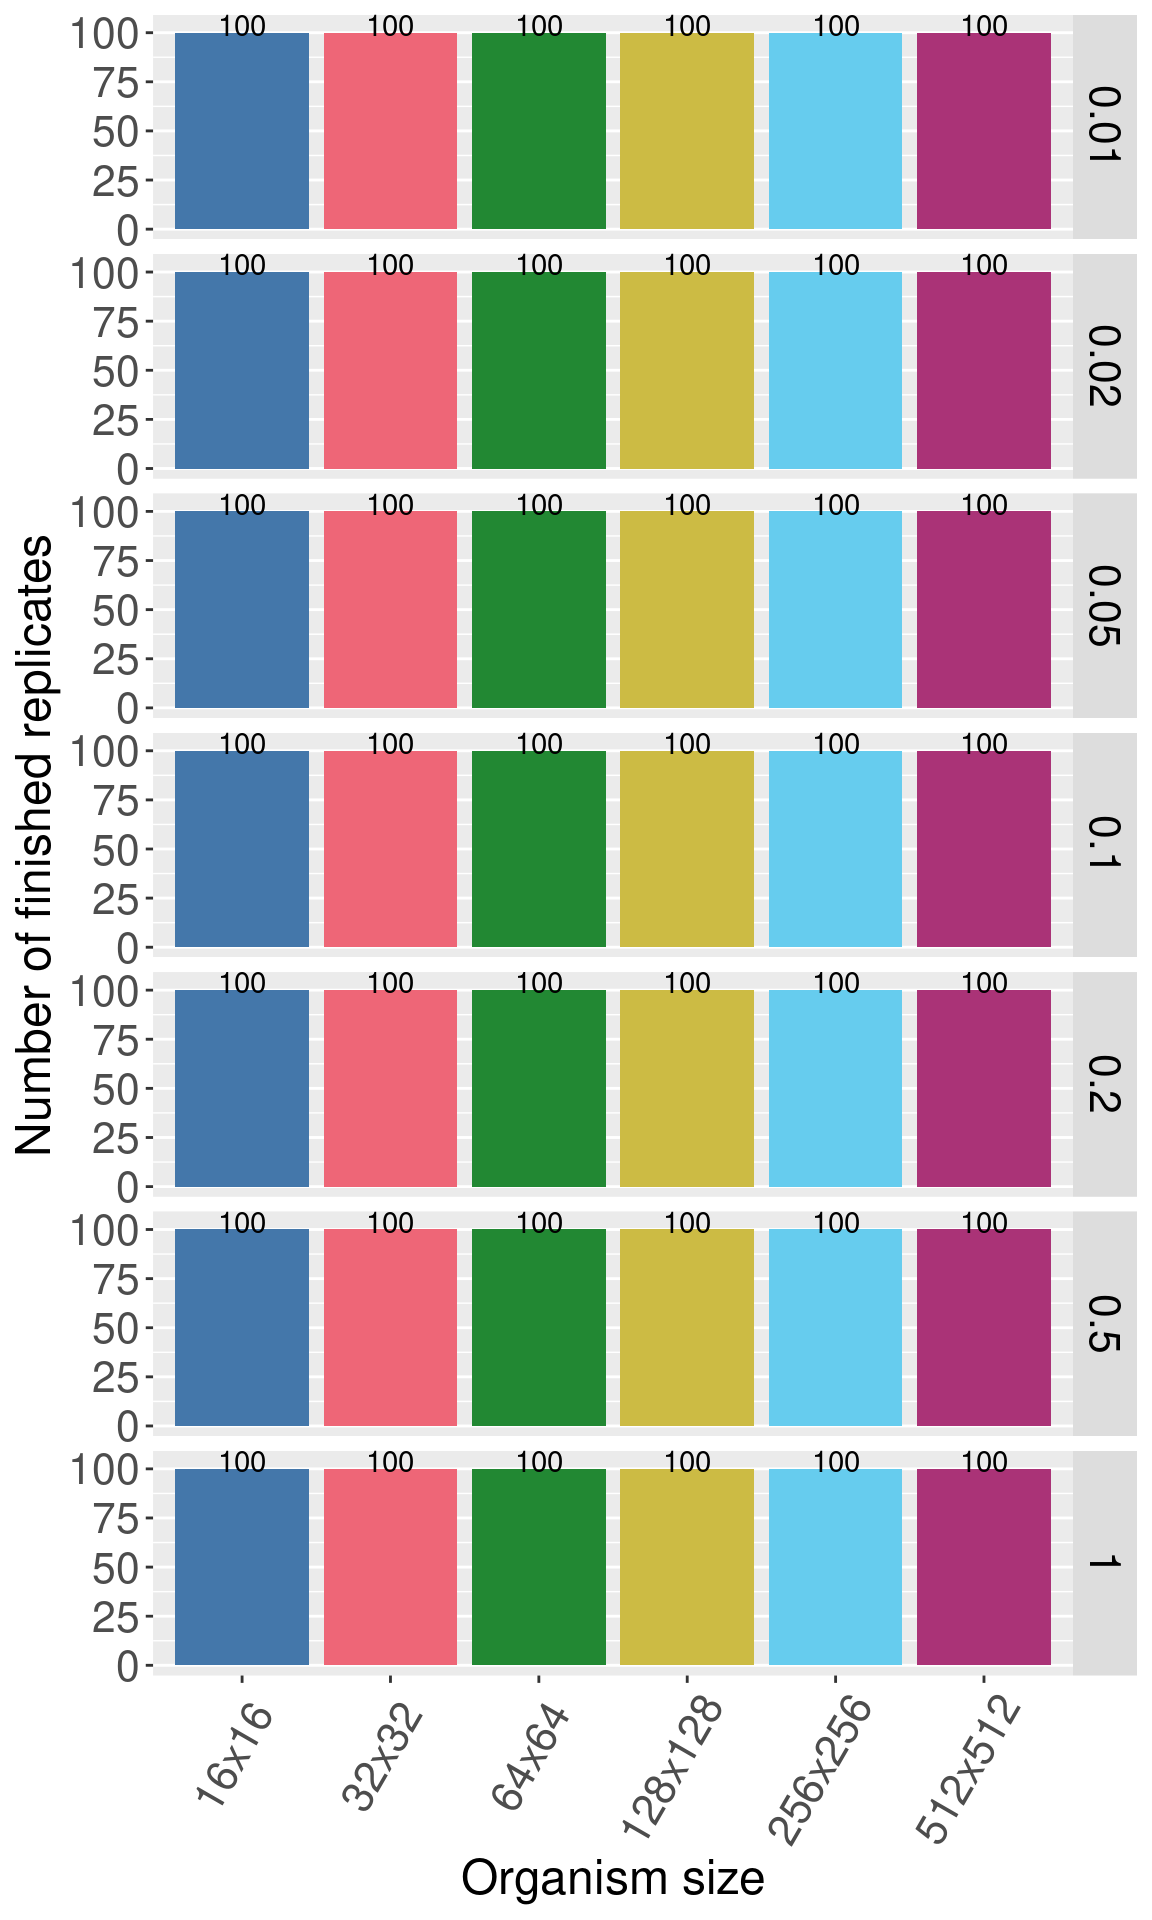
\includegraphics{primordium_supplemental_material_files/figure-latex/unnamed-chunk-5-1.pdf}

\hypertarget{aggregate-plots}{%
\section{Aggregate plots}\label{aggregate-plots}}

Here we plot all the data at once.

\hypertarget{boxplots}{%
\subsection{Boxplots}\label{boxplots}}

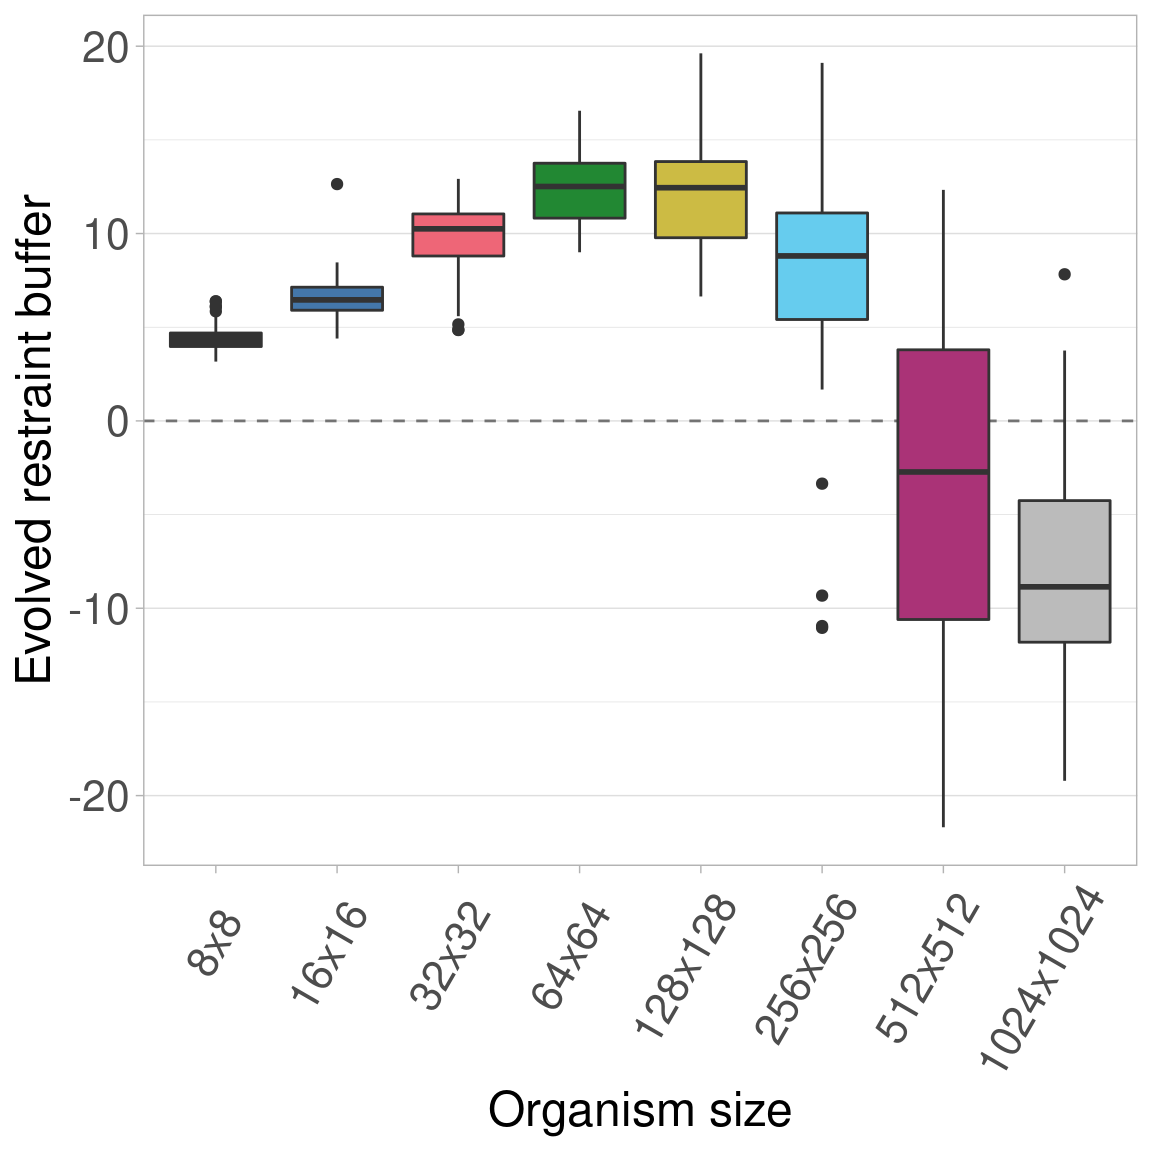
\includegraphics{primordium_supplemental_material_files/figure-latex/unnamed-chunk-6-1.pdf}

\hypertarget{raincloud-plots}{%
\subsection{Raincloud plots}\label{raincloud-plots}}

We can plot the same data via raincloud plots.

\begin{verbatim}
## Picking joint bandwidth of 1.16
\end{verbatim}

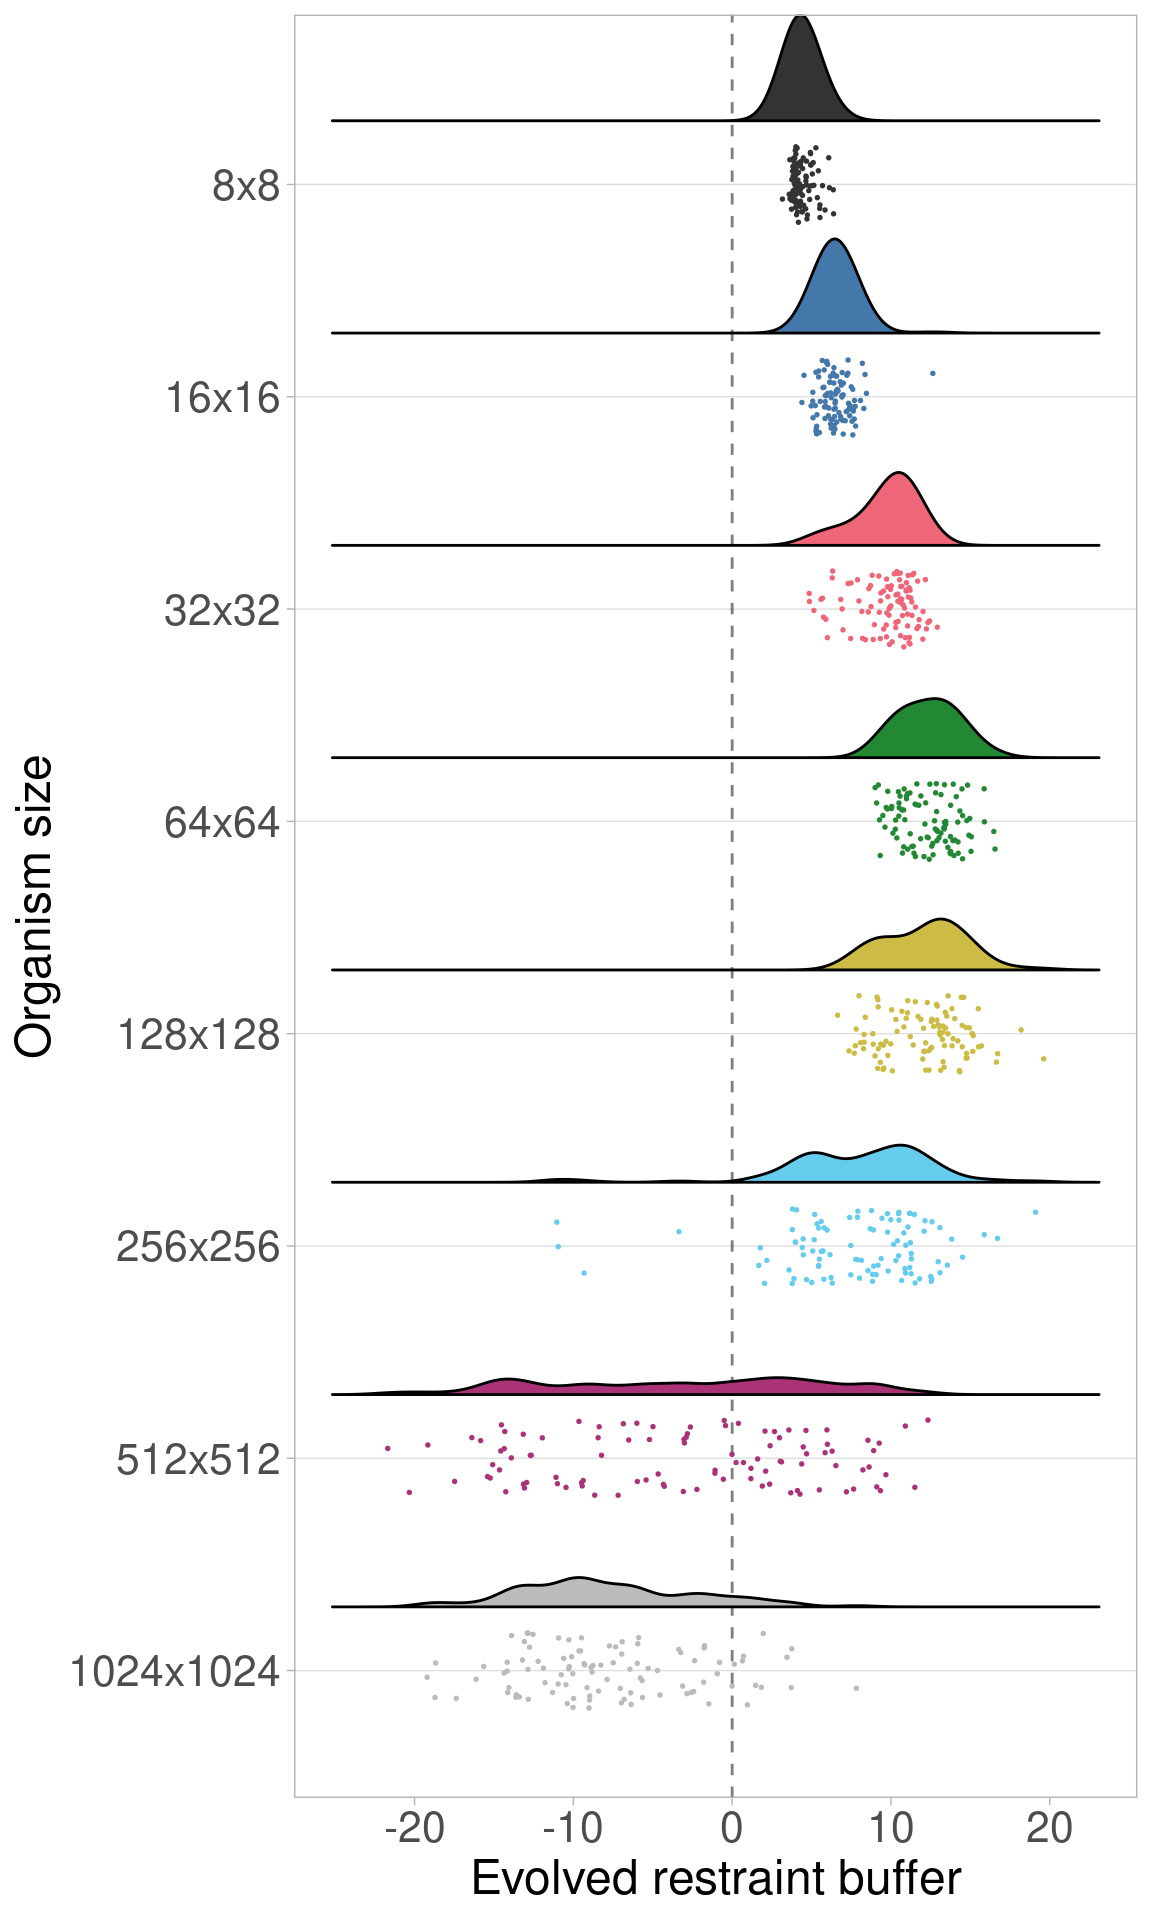
\includegraphics{primordium_supplemental_material_files/figure-latex/unnamed-chunk-7-1.pdf}

\hypertarget{statistics}{%
\section{Statistics}\label{statistics}}

First, we perform a Kruskal-Wallis test across all organism sizes to indicate if variance exists.
If variance exists, we then perform a pairwise Wilcoxon Rank-Sum test to show which pairs of organism sizes significantly differ.
Finally, we perform Bonferroni-Holm corrections for multiple comparisons.

\begin{Shaded}
\begin{Highlighting}[]
\NormalTok{  res =}\StringTok{ }\KeywordTok{kruskal.test}\NormalTok{(df2}\OperatorTok{$}\NormalTok{restraint\_value }\OperatorTok{\textasciitilde{}}\StringTok{ }\NormalTok{df2}\OperatorTok{$}\NormalTok{MCSIZE, df2)}
\NormalTok{  df\_kruskal =}\StringTok{ }\KeywordTok{data.frame}\NormalTok{(}\DataTypeTok{data =} \KeywordTok{matrix}\NormalTok{(}\DataTypeTok{nrow =} \DecValTok{0}\NormalTok{, }\DataTypeTok{ncol =} \DecValTok{3}\NormalTok{))}
  \KeywordTok{colnames}\NormalTok{(df\_kruskal) =}\StringTok{ }\KeywordTok{c}\NormalTok{(}\StringTok{\textquotesingle{}p\_value\textquotesingle{}}\NormalTok{, }\StringTok{\textquotesingle{}chi\_squared\textquotesingle{}}\NormalTok{, }\StringTok{\textquotesingle{}df\textquotesingle{}}\NormalTok{)}
\NormalTok{  df\_kruskal[}\KeywordTok{nrow}\NormalTok{(df\_kruskal) }\OperatorTok{+}\StringTok{ }\DecValTok{1}\NormalTok{,] =}\StringTok{ }\KeywordTok{c}\NormalTok{(res}\OperatorTok{$}\NormalTok{p.value, }\KeywordTok{as.numeric}\NormalTok{(res}\OperatorTok{$}\NormalTok{statistic)[}\DecValTok{1}\NormalTok{], }\KeywordTok{as.numeric}\NormalTok{(res}\OperatorTok{$}\NormalTok{parameter)[}\DecValTok{1}\NormalTok{])}
\NormalTok{  df\_kruskal}\OperatorTok{$}\NormalTok{less\_}\FloatTok{0.01}\NormalTok{ =}\StringTok{ }\NormalTok{df\_kruskal}\OperatorTok{$}\NormalTok{p\_value }\OperatorTok{\textless{}}\StringTok{ }\FloatTok{0.01}
  \KeywordTok{print}\NormalTok{(df\_kruskal)}
\end{Highlighting}
\end{Shaded}

\begin{verbatim}
##         p_value chi_squared df less_0.01
## 1 1.506351e-127    610.2553  7      TRUE
\end{verbatim}

We see that significant variation exists, so we perform pairwise Wilcoxon tests on each to see which pairs of sizes are significantly different.

\begin{Shaded}
\begin{Highlighting}[]
\NormalTok{size\_vec =}\StringTok{ }\KeywordTok{c}\NormalTok{(}\DecValTok{16}\NormalTok{, }\DecValTok{32}\NormalTok{, }\DecValTok{64}\NormalTok{, }\DecValTok{128}\NormalTok{, }\DecValTok{256}\NormalTok{, }\DecValTok{512}\NormalTok{)}
\NormalTok{df\_test =}\StringTok{ }\NormalTok{df2}
\NormalTok{df\_wilcox =}\StringTok{ }\KeywordTok{data.frame}\NormalTok{(}\DataTypeTok{data =} \KeywordTok{matrix}\NormalTok{(}\DataTypeTok{nrow =} \DecValTok{0}\NormalTok{, }\DataTypeTok{ncol =} \DecValTok{5}\NormalTok{))}
\KeywordTok{colnames}\NormalTok{(df\_wilcox) =}\StringTok{ }\KeywordTok{c}\NormalTok{(}\StringTok{\textquotesingle{}size\_a\textquotesingle{}}\NormalTok{, }\StringTok{\textquotesingle{}size\_b\textquotesingle{}}\NormalTok{, }\StringTok{\textquotesingle{}p\_value\_corrected\textquotesingle{}}\NormalTok{, }\StringTok{\textquotesingle{}p\_value\_raw\textquotesingle{}}\NormalTok{, }\StringTok{\textquotesingle{}W\textquotesingle{}}\NormalTok{)}
\ControlFlowTok{for}\NormalTok{(size\_idx\_a }\ControlFlowTok{in} \DecValTok{1}\OperatorTok{:}\NormalTok{(}\KeywordTok{length}\NormalTok{(size\_vec) }\OperatorTok{{-}}\StringTok{ }\DecValTok{1}\NormalTok{))\{}
\NormalTok{  size\_a =}\StringTok{ }\NormalTok{size\_vec[size\_idx\_a]}
  \ControlFlowTok{for}\NormalTok{(size\_idx\_b }\ControlFlowTok{in}\NormalTok{ (size\_idx\_a }\OperatorTok{+}\StringTok{ }\DecValTok{1}\NormalTok{)}\OperatorTok{:}\KeywordTok{length}\NormalTok{(size\_vec))\{}
\NormalTok{    size\_b =}\StringTok{ }\NormalTok{size\_vec[size\_idx\_b]}
\NormalTok{    res =}\StringTok{ }\KeywordTok{wilcox.test}\NormalTok{(df\_test[df\_test}\OperatorTok{$}\NormalTok{MCSIZE }\OperatorTok{==}\StringTok{ }\NormalTok{size\_a,]}\OperatorTok{$}\NormalTok{restraint\_value, df\_test[df\_test}\OperatorTok{$}\NormalTok{MCSIZE }\OperatorTok{==}\StringTok{ }\NormalTok{size\_b,]}\OperatorTok{$}\NormalTok{restraint\_value, }\DataTypeTok{alternative =} \StringTok{\textquotesingle{}two.sided\textquotesingle{}}\NormalTok{) }
\NormalTok{    df\_wilcox[}\KeywordTok{nrow}\NormalTok{(df\_wilcox) }\OperatorTok{+}\StringTok{ }\DecValTok{1}\NormalTok{,] =}\StringTok{ }\KeywordTok{c}\NormalTok{(size\_a, size\_b, }\DecValTok{0}\NormalTok{, res}\OperatorTok{$}\NormalTok{p.value, }\KeywordTok{as.numeric}\NormalTok{(res}\OperatorTok{$}\NormalTok{statistic)[}\DecValTok{1}\NormalTok{])}
\NormalTok{  \}}
\NormalTok{\}}
\NormalTok{df\_wilcox}\OperatorTok{$}\NormalTok{p\_value\_corrected =}\StringTok{ }\KeywordTok{p.adjust}\NormalTok{(df\_wilcox}\OperatorTok{$}\NormalTok{p\_value\_raw, }\DataTypeTok{method =} \StringTok{\textquotesingle{}holm\textquotesingle{}}\NormalTok{)}
\NormalTok{df\_wilcox}\OperatorTok{$}\NormalTok{less\_}\FloatTok{0.01}\NormalTok{ =}\StringTok{ }\NormalTok{df\_wilcox}\OperatorTok{$}\NormalTok{p\_value\_corrected }\OperatorTok{\textless{}}\StringTok{ }\FloatTok{0.01}
\KeywordTok{print}\NormalTok{(df\_wilcox)}
\end{Highlighting}
\end{Shaded}

\begin{verbatim}
##    size_a size_b p_value_corrected  p_value_raw      W less_0.01
## 1      16     32      4.406735e-21 4.406735e-22 1045.5      TRUE
## 2      16     64      1.790650e-32 1.193767e-33   51.5      TRUE
## 3      16    128      2.585339e-31 1.988723e-32  147.0      TRUE
## 4      16    256      1.864978e-03 6.216595e-04 3599.0      TRUE
## 5      16    512      3.596138e-17 4.495172e-18 8547.0      TRUE
## 6      32     64      2.103060e-15 3.004372e-16 1654.5      TRUE
## 7      32    128      1.857809e-09 4.644523e-10 2449.5      TRUE
## 8      32    256      8.472946e-03 4.236473e-03 6171.0      TRUE
## 9      32    512      1.338207e-26 1.216552e-27 9459.5      TRUE
## 10     64    128      4.429461e-01 4.429461e-01 5314.5     FALSE
## 11     64    256      2.515682e-15 4.192803e-16 8329.0      TRUE
## 12     64    512      1.552625e-31 1.109018e-32 9873.0      TRUE
## 13    128    256      4.763656e-12 9.527311e-13 7921.5      TRUE
## 14    128    512      3.610598e-30 3.008832e-31 9759.0      TRUE
## 15    256    512      7.155324e-19 7.950361e-20 8730.5      TRUE
\end{verbatim}

\hypertarget{somatic-mutation-rate-sweep}{%
\chapter{Somatic Mutation Rate Sweep}\label{somatic-mutation-rate-sweep}}

This was one of the preliminary experiments we conducted to find the default parameters for Primordium.
However, the data shown here were ran after the system was finalized (with new random number seeds).
There were no qualitative differences from prior results.

Here, we vary the \emph{somatic} mutation rate, which is the probability that cell replication will result in a mutation to the offspring's genome.
The probability of a mutation is per-genome, not per-bit.
When a somatic mutation occurs, only a change of +/-1 is possible in the restraint value.
We settled on a somatic mutation rate of 0.5 (\emph{i.e.}, each cell replication has a 50\% chance of mutation).

The configuration script and data for the experiment can be found under \texttt{2021\_02\_27\_\_soma\_mut\_fin/} in the experiments directory of the git repository.

\hypertarget{data-cleaning-1}{%
\section{Data cleaning}\label{data-cleaning-1}}

Load necessary libraries

\begin{Shaded}
\begin{Highlighting}[]
\KeywordTok{library}\NormalTok{(dplyr)}
\KeywordTok{library}\NormalTok{(ggplot2)}
\KeywordTok{library}\NormalTok{(ggridges)}
\KeywordTok{library}\NormalTok{(scales)}
\KeywordTok{library}\NormalTok{(khroma)}
\end{Highlighting}
\end{Shaded}

Load the data and trim include only the final generation data for sizes 16x16 to 512x512.

\begin{Shaded}
\begin{Highlighting}[]
\CommentTok{\# Load the data}
\NormalTok{df =}\StringTok{ }\KeywordTok{read.csv}\NormalTok{(}\StringTok{\textquotesingle{}../experiments/2021\_02\_27\_\_soma\_mut\_fin/evolution/data/scraped\_evolution\_data.csv\textquotesingle{}}\NormalTok{)}
\CommentTok{\# Trim off NAs (artifacts of how we scraped the data) and trim to only have gen 10,000}
\NormalTok{df2 =}\StringTok{ }\NormalTok{df[}\OperatorTok{!}\KeywordTok{is.na}\NormalTok{(df}\OperatorTok{$}\NormalTok{MCSIZE) }\OperatorTok{\&}\StringTok{ }\NormalTok{df}\OperatorTok{$}\NormalTok{generation }\OperatorTok{==}\StringTok{ }\DecValTok{10000}\NormalTok{,]}
\CommentTok{\# Ignore data for size 8x8 and 1024x1024}
\NormalTok{df2 =}\StringTok{ }\NormalTok{df2[df2}\OperatorTok{$}\NormalTok{MCSIZE }\OperatorTok{!=}\StringTok{ }\DecValTok{8} \OperatorTok{\&}\StringTok{ }\NormalTok{df2}\OperatorTok{$}\NormalTok{MCSIZE }\OperatorTok{!=}\StringTok{ }\DecValTok{1024}\NormalTok{,]}
\end{Highlighting}
\end{Shaded}

We group and summarize the data to ensure all replicates are present.

\begin{Shaded}
\begin{Highlighting}[]
\CommentTok{\# Group the data by size and summarize}
\NormalTok{data\_grouped =}\StringTok{ }\NormalTok{dplyr}\OperatorTok{::}\KeywordTok{group\_by}\NormalTok{(df2, MCSIZE, CELLMUT)}
\NormalTok{data\_summary =}\StringTok{ }\NormalTok{dplyr}\OperatorTok{::}\KeywordTok{summarize}\NormalTok{(data\_grouped, }\DataTypeTok{mean\_ones =} \KeywordTok{mean}\NormalTok{(ave\_ones), }\DataTypeTok{n =}\NormalTok{ dplyr}\OperatorTok{::}\KeywordTok{n}\NormalTok{())}
\end{Highlighting}
\end{Shaded}

\begin{verbatim}
## `summarise()` has grouped output by 'MCSIZE'. You can override using the `.groups` argument.
\end{verbatim}

We clean the data and create a few helper variables to make plotting easier.

\begin{Shaded}
\begin{Highlighting}[]
\CommentTok{\# Calculate restraint value (x {-} 60 because genome length is 100 here)}
\NormalTok{df2}\OperatorTok{$}\NormalTok{restraint\_value =}\StringTok{ }\NormalTok{df2}\OperatorTok{$}\NormalTok{ave\_ones }\OperatorTok{{-}}\StringTok{ }\DecValTok{60}
\CommentTok{\# Make a nice, clean factor for size}
\NormalTok{df2}\OperatorTok{$}\NormalTok{size\_str =}\StringTok{ }\KeywordTok{paste0}\NormalTok{(df2}\OperatorTok{$}\NormalTok{MCSIZE, }\StringTok{\textquotesingle{}x\textquotesingle{}}\NormalTok{, df2}\OperatorTok{$}\NormalTok{MCSIZE)}
\NormalTok{df2}\OperatorTok{$}\NormalTok{size\_factor =}\StringTok{ }\KeywordTok{factor}\NormalTok{(df2}\OperatorTok{$}\NormalTok{size\_str, }\DataTypeTok{levels =} \KeywordTok{c}\NormalTok{(}\StringTok{\textquotesingle{}16x16\textquotesingle{}}\NormalTok{, }\StringTok{\textquotesingle{}32x32\textquotesingle{}}\NormalTok{, }\StringTok{\textquotesingle{}64x64\textquotesingle{}}\NormalTok{, }\StringTok{\textquotesingle{}128x128\textquotesingle{}}\NormalTok{, }\StringTok{\textquotesingle{}256x256\textquotesingle{}}\NormalTok{, }\StringTok{\textquotesingle{}512x512\textquotesingle{}}\NormalTok{, }\StringTok{\textquotesingle{}1024x1024\textquotesingle{}}\NormalTok{))}
\NormalTok{df2}\OperatorTok{$}\NormalTok{size\_factor\_reversed =}\StringTok{ }\KeywordTok{factor}\NormalTok{(df2}\OperatorTok{$}\NormalTok{size\_str, }\DataTypeTok{levels =} \KeywordTok{rev}\NormalTok{(}\KeywordTok{c}\NormalTok{(}\StringTok{\textquotesingle{}16x16\textquotesingle{}}\NormalTok{, }\StringTok{\textquotesingle{}32x32\textquotesingle{}}\NormalTok{, }\StringTok{\textquotesingle{}64x64\textquotesingle{}}\NormalTok{, }\StringTok{\textquotesingle{}128x128\textquotesingle{}}\NormalTok{, }\StringTok{\textquotesingle{}256x256\textquotesingle{}}\NormalTok{, }\StringTok{\textquotesingle{}512x512\textquotesingle{}}\NormalTok{, }\StringTok{\textquotesingle{}1024x1024\textquotesingle{}}\NormalTok{)))}
\NormalTok{df2}\OperatorTok{$}\NormalTok{soma\_mut\_str =}\StringTok{ }\KeywordTok{paste}\NormalTok{(}\StringTok{\textquotesingle{}soma CELLMUT\textquotesingle{}}\NormalTok{, df2}\OperatorTok{$}\NormalTok{CELLMUT)}
\NormalTok{df2}\OperatorTok{$}\NormalTok{mut\_factor =}\StringTok{ }\KeywordTok{factor}\NormalTok{(df2}\OperatorTok{$}\NormalTok{CELLMUT, }\DataTypeTok{levels =} \KeywordTok{c}\NormalTok{(}\FloatTok{0.01}\NormalTok{, }\FloatTok{0.02}\NormalTok{, }\FloatTok{0.05}\NormalTok{, }\FloatTok{0.10}\NormalTok{, }\FloatTok{0.20}\NormalTok{, }\FloatTok{0.50}\NormalTok{, }\FloatTok{1.00}\NormalTok{))}
\NormalTok{data\_summary}\OperatorTok{$}\NormalTok{size\_str =}\StringTok{ }\KeywordTok{paste0}\NormalTok{(data\_summary}\OperatorTok{$}\NormalTok{MCSIZE, }\StringTok{\textquotesingle{}x\textquotesingle{}}\NormalTok{, data\_summary}\OperatorTok{$}\NormalTok{MCSIZE)}
\NormalTok{data\_summary}\OperatorTok{$}\NormalTok{size\_factor =}\StringTok{ }\KeywordTok{factor}\NormalTok{(data\_summary}\OperatorTok{$}\NormalTok{size\_str, }\DataTypeTok{levels =} \KeywordTok{c}\NormalTok{(}\StringTok{\textquotesingle{}16x16\textquotesingle{}}\NormalTok{, }\StringTok{\textquotesingle{}32x32\textquotesingle{}}\NormalTok{, }\StringTok{\textquotesingle{}64x64\textquotesingle{}}\NormalTok{, }\StringTok{\textquotesingle{}128x128\textquotesingle{}}\NormalTok{, }\StringTok{\textquotesingle{}256x256\textquotesingle{}}\NormalTok{, }\StringTok{\textquotesingle{}512x512\textquotesingle{}}\NormalTok{, }\StringTok{\textquotesingle{}1024x1024\textquotesingle{}}\NormalTok{))}
\NormalTok{data\_summary}\OperatorTok{$}\NormalTok{soma\_mut\_str =}\StringTok{ }\KeywordTok{paste}\NormalTok{(}\StringTok{\textquotesingle{}soma CELLMUT\textquotesingle{}}\NormalTok{, data\_summary}\OperatorTok{$}\NormalTok{CELLMUT)}
\NormalTok{data\_summary}\OperatorTok{$}\NormalTok{mut\_factor =}\StringTok{ }\KeywordTok{factor}\NormalTok{(data\_summary}\OperatorTok{$}\NormalTok{CELLMUT, }\DataTypeTok{levels =} \KeywordTok{c}\NormalTok{(}\FloatTok{0.01}\NormalTok{, }\FloatTok{0.02}\NormalTok{, }\FloatTok{0.05}\NormalTok{, }\FloatTok{0.10}\NormalTok{, }\FloatTok{0.20}\NormalTok{, }\FloatTok{0.50}\NormalTok{, }\FloatTok{1.00}\NormalTok{))}
\CommentTok{\# Create a map of colors we\textquotesingle{}ll use to plot the different organism sizes}
\NormalTok{color\_vec =}\StringTok{ }\KeywordTok{as.character}\NormalTok{(khroma}\OperatorTok{::}\KeywordTok{color}\NormalTok{(}\StringTok{\textquotesingle{}bright\textquotesingle{}}\NormalTok{)(}\DecValTok{7}\NormalTok{))}
\NormalTok{color\_map =}\StringTok{ }\KeywordTok{c}\NormalTok{(}
  \StringTok{\textquotesingle{}16x16\textquotesingle{}}\NormalTok{ =}\StringTok{     }\NormalTok{color\_vec[}\DecValTok{1}\NormalTok{],}
  \StringTok{\textquotesingle{}32x32\textquotesingle{}}\NormalTok{ =}\StringTok{     }\NormalTok{color\_vec[}\DecValTok{2}\NormalTok{],}
  \StringTok{\textquotesingle{}64x64\textquotesingle{}}\NormalTok{ =}\StringTok{     }\NormalTok{color\_vec[}\DecValTok{3}\NormalTok{],}
  \StringTok{\textquotesingle{}128x128\textquotesingle{}}\NormalTok{ =}\StringTok{   }\NormalTok{color\_vec[}\DecValTok{4}\NormalTok{],}
  \StringTok{\textquotesingle{}256x256\textquotesingle{}}\NormalTok{ =}\StringTok{   }\NormalTok{color\_vec[}\DecValTok{5}\NormalTok{],}
  \StringTok{\textquotesingle{}512x512\textquotesingle{}}\NormalTok{ =}\StringTok{   }\NormalTok{color\_vec[}\DecValTok{6}\NormalTok{],}
  \StringTok{\textquotesingle{}1024x1024\textquotesingle{}}\NormalTok{ =}\StringTok{ }\NormalTok{color\_vec[}\DecValTok{7}\NormalTok{]}
\NormalTok{)}
\CommentTok{\# Set the sizes for text in plots}
\NormalTok{text\_major\_size =}\StringTok{ }\DecValTok{18}
\NormalTok{text\_minor\_size =}\StringTok{ }\DecValTok{16} 
\end{Highlighting}
\end{Shaded}

\hypertarget{data-integrity-check-1}{%
\section{Data integrity check}\label{data-integrity-check-1}}

Now we plot the number of finished replicates for each treatment to make sure all data are present.
Each row shows a different somatic mutation rate.
Each bar/color shows a different organism size.
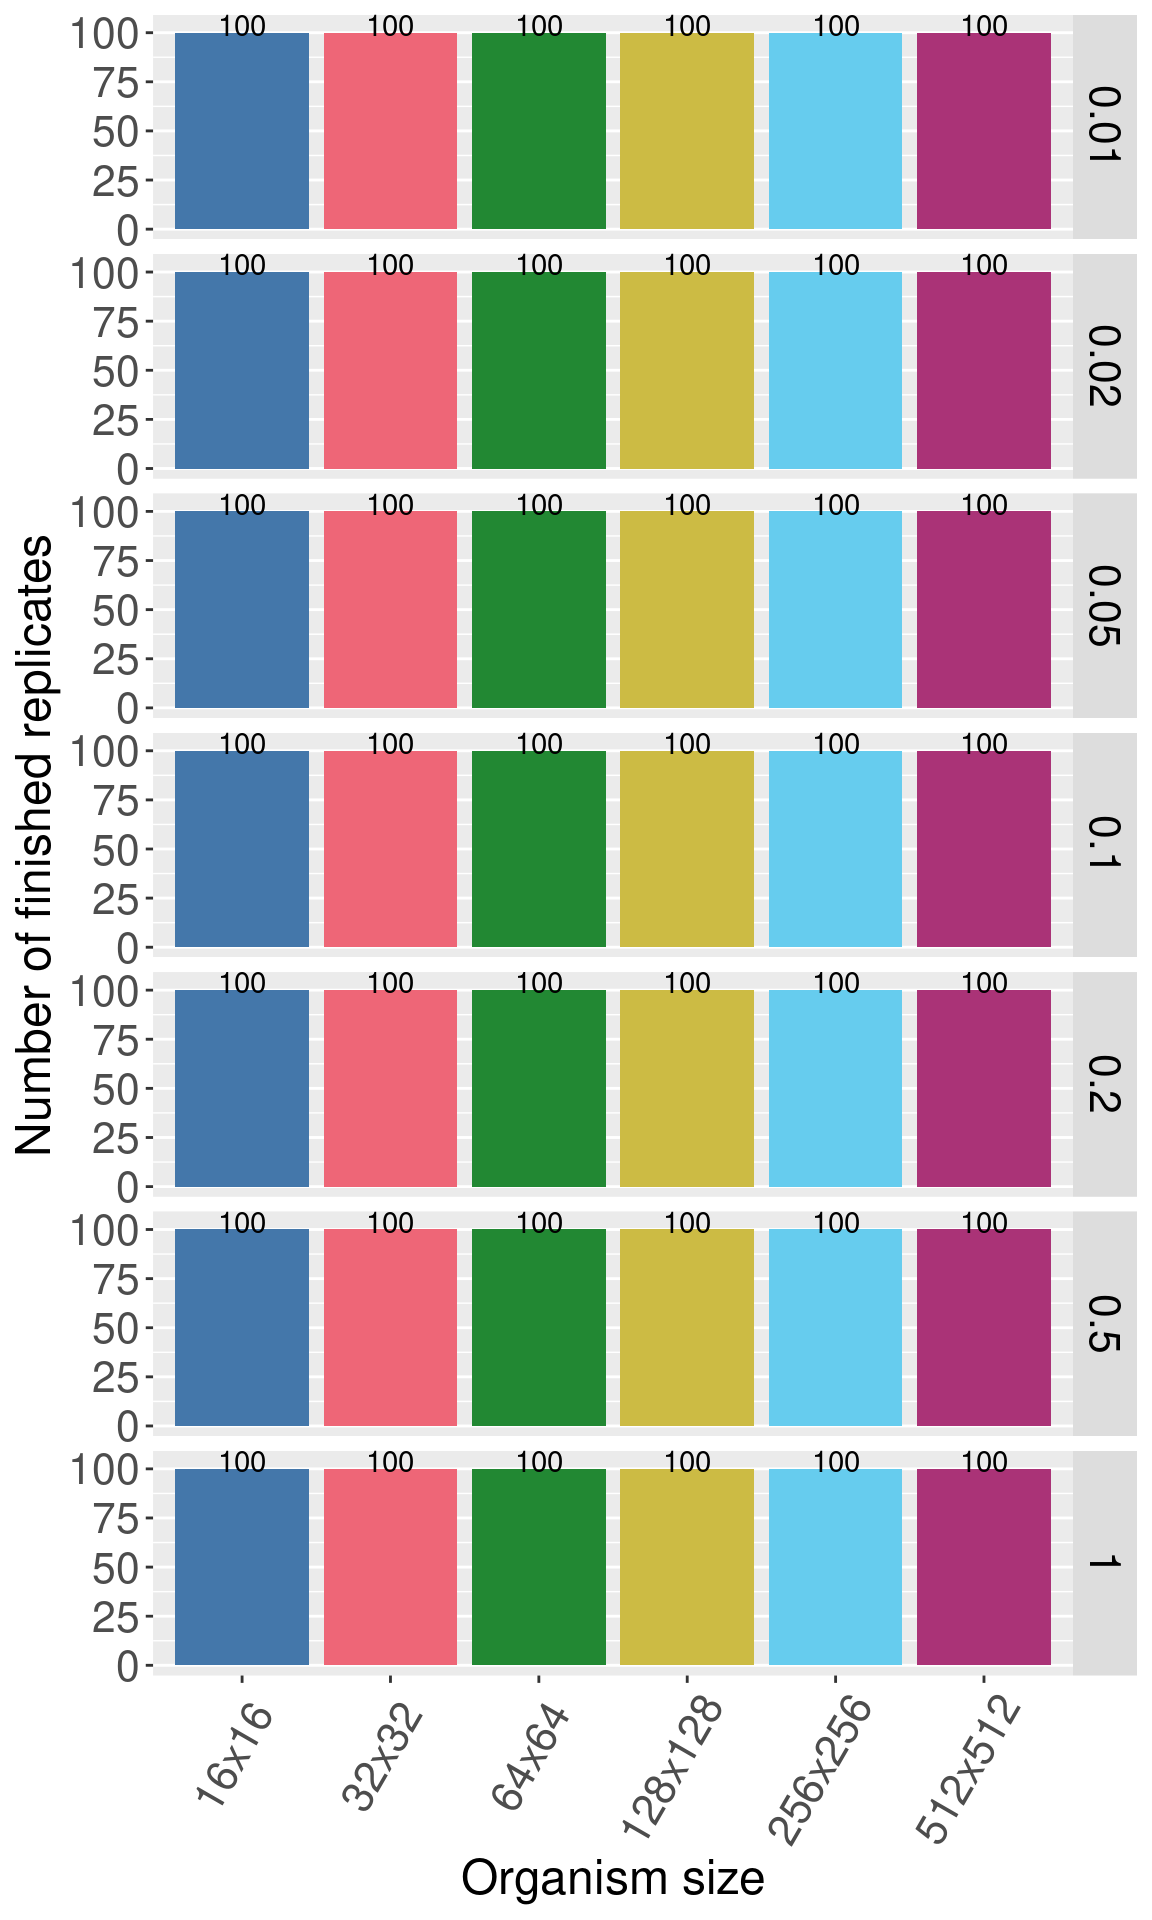
\includegraphics{primordium_supplemental_material_files/figure-latex/unnamed-chunk-14-1.pdf}

\hypertarget{aggregate-plots-1}{%
\section{Aggregate plots}\label{aggregate-plots-1}}

\hypertarget{facet-by-somatic-mutation-rate}{%
\subsection{Facet by somatic mutation rate}\label{facet-by-somatic-mutation-rate}}

Here we plot all the data at once.
Each row showing a different somatic mutation rate and each boxplot shows a given organism size.
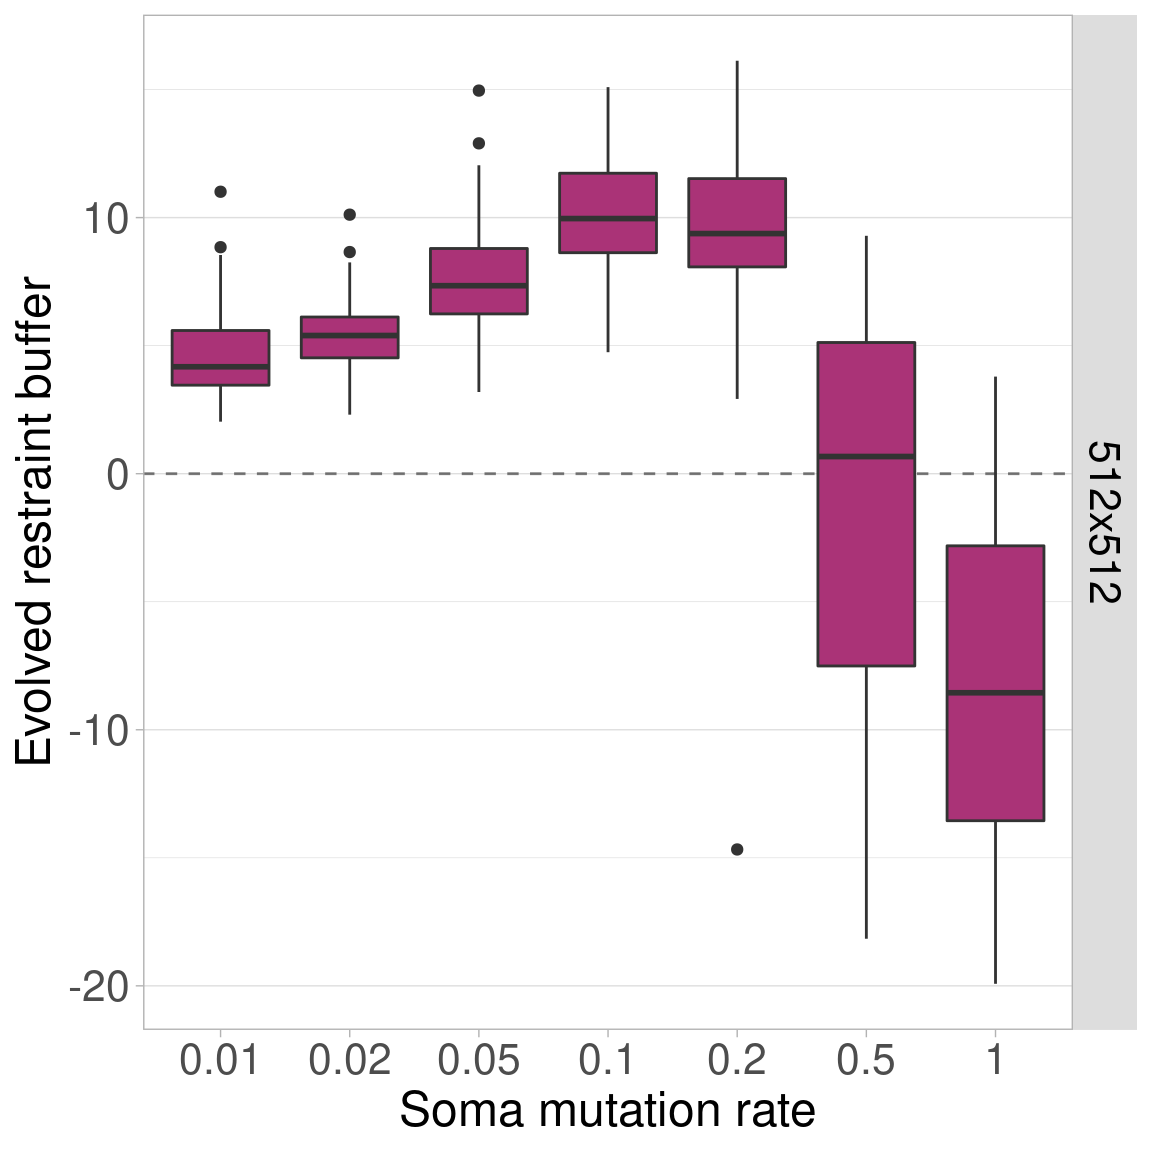
\includegraphics{primordium_supplemental_material_files/figure-latex/unnamed-chunk-15-1.pdf}

Here we plot the same data, only we allow the y-axis to vary between rows.
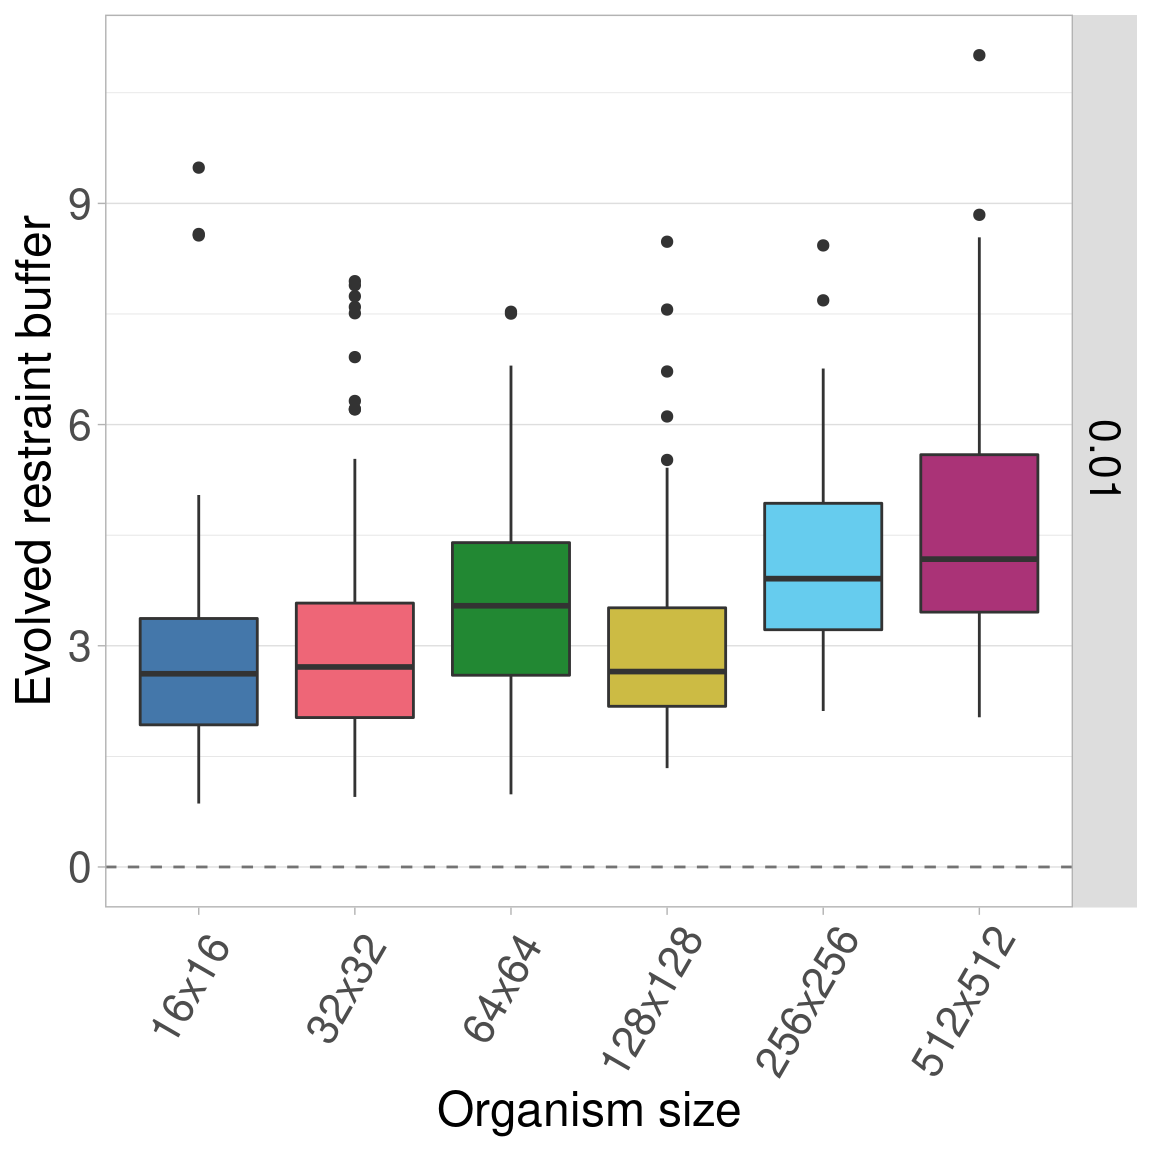
\includegraphics{primordium_supplemental_material_files/figure-latex/unnamed-chunk-16-1.pdf}

\hypertarget{facet-by-organism-size}{%
\subsection{Facet by organism size}\label{facet-by-organism-size}}

Next, we plot the same data, but this time each row corresponds to a certain organism size, while somatic mutation rate changes along the x-axis.
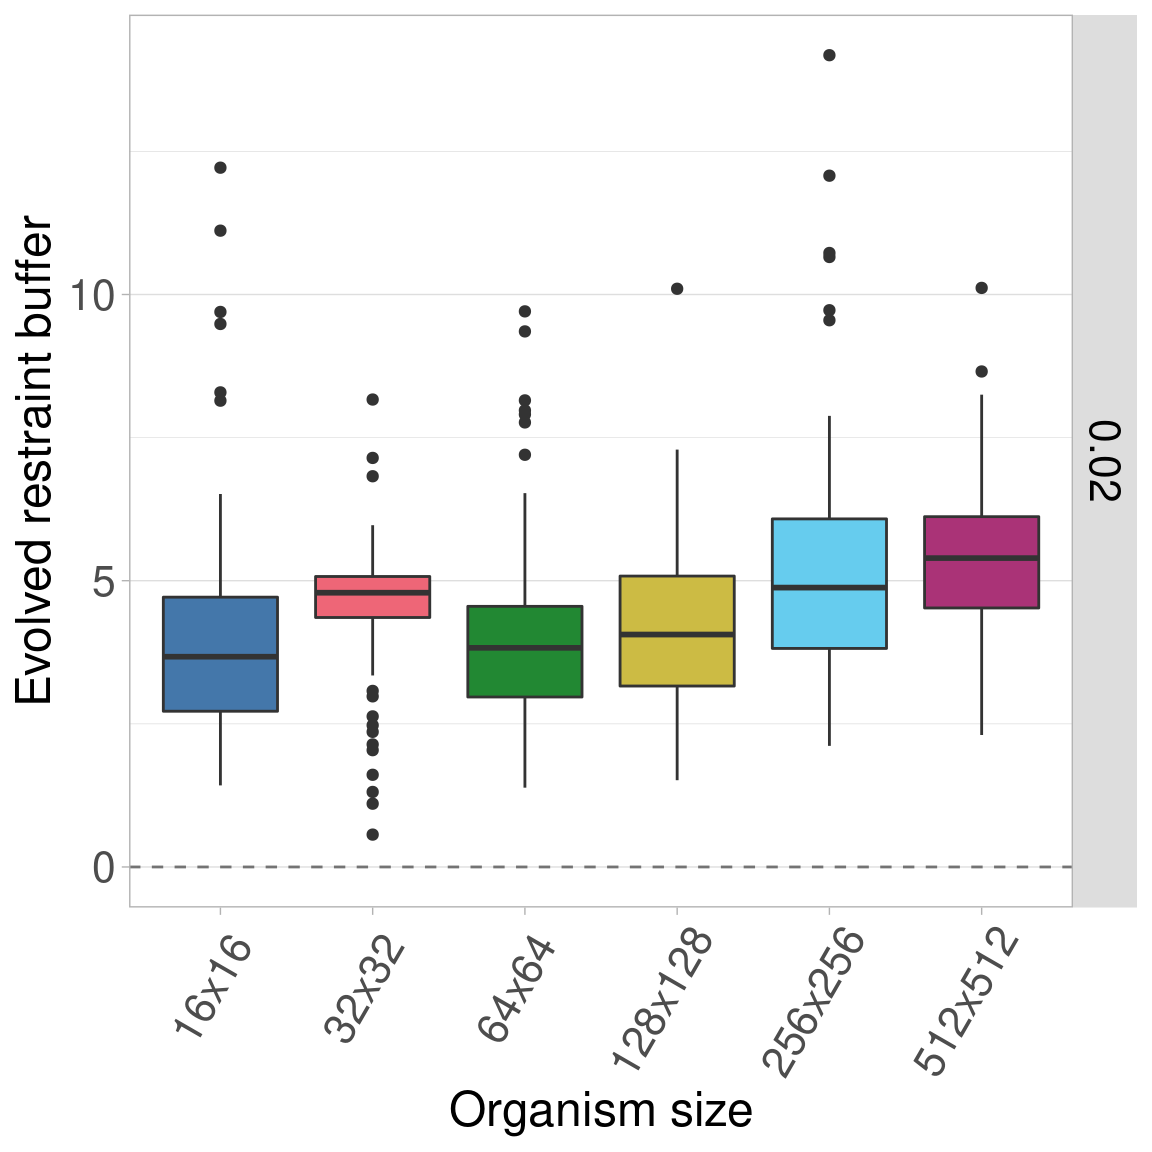
\includegraphics{primordium_supplemental_material_files/figure-latex/unnamed-chunk-17-1.pdf}

Again, we replot the same data but allow the y-axis to vary between rows.
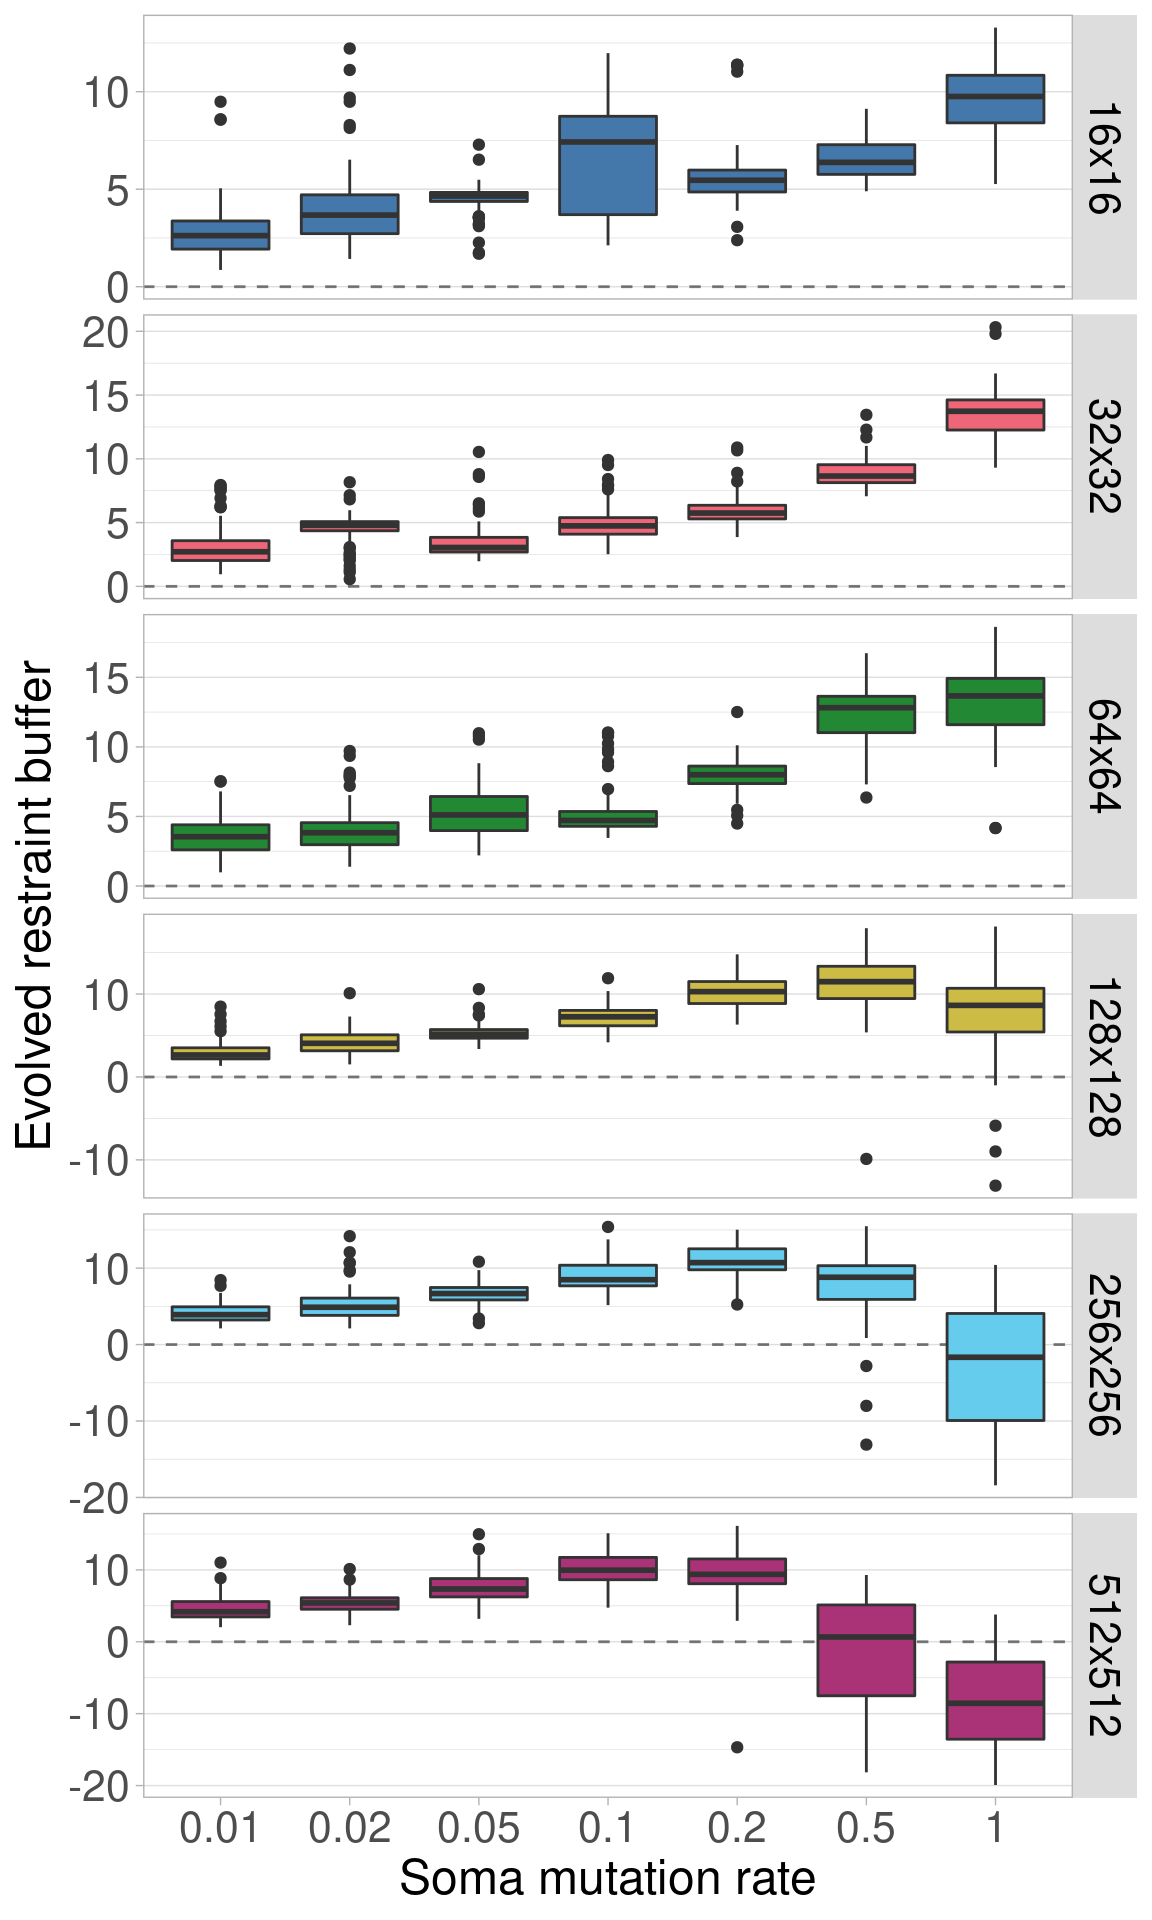
\includegraphics{primordium_supplemental_material_files/figure-latex/unnamed-chunk-18-1.pdf}

\hypertarget{single-organism-size-plots}{%
\section{Single organism size plots}\label{single-organism-size-plots}}

Here we plot each organism size independently, with the somatic mutation rate on the x-axis.

\hypertarget{organism-size-16x16}{%
\subsection{Organism size 16x16}\label{organism-size-16x16}}

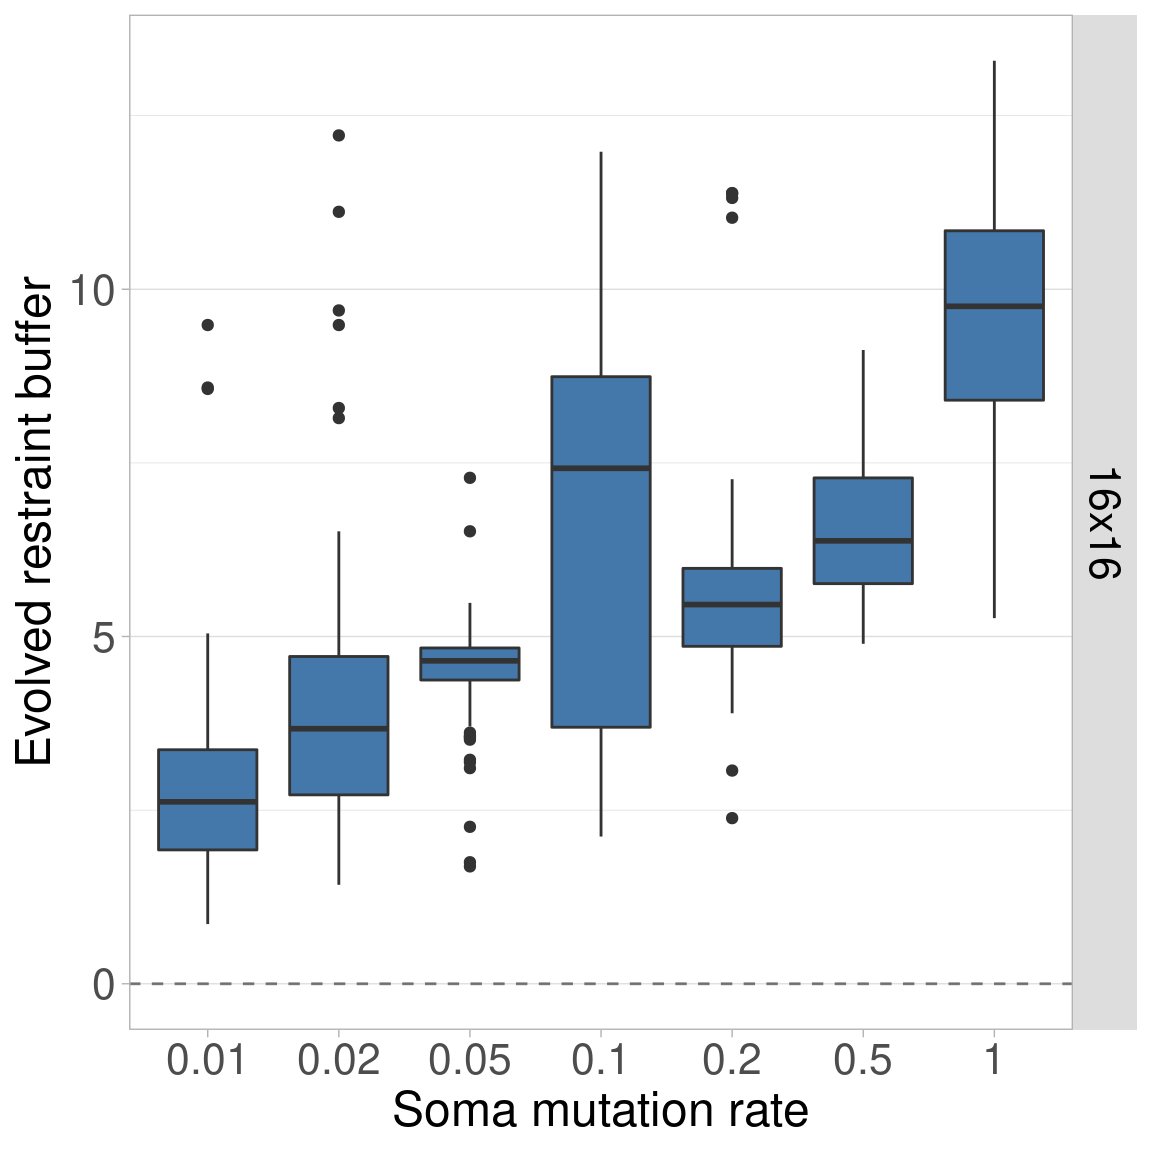
\includegraphics{primordium_supplemental_material_files/figure-latex/unnamed-chunk-19-1.pdf}

\hypertarget{organism-size-32x32}{%
\subsection{Organism size 32x32}\label{organism-size-32x32}}

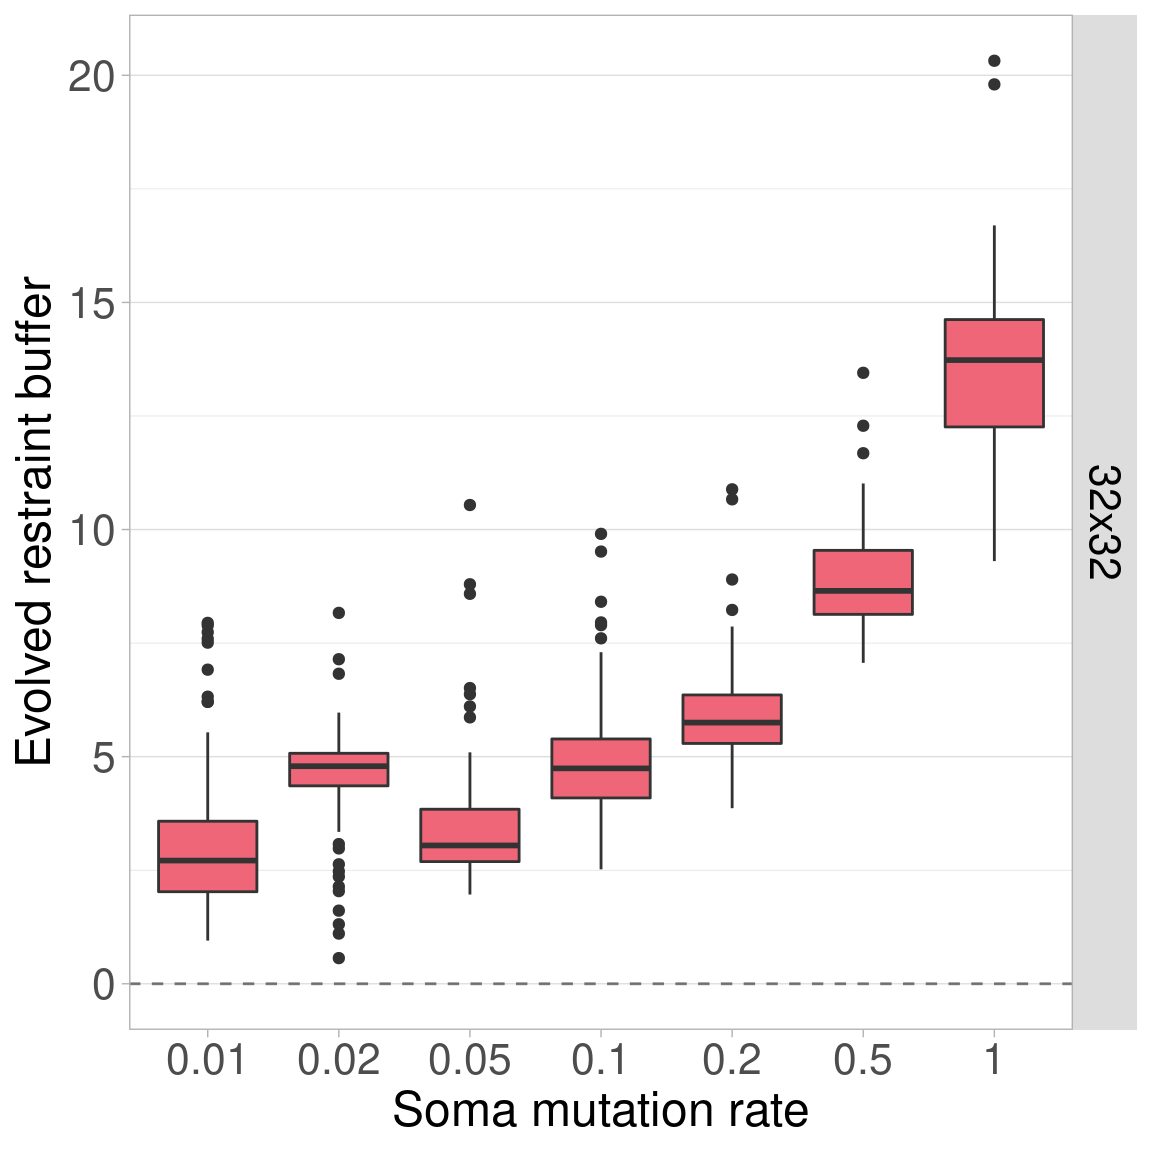
\includegraphics{primordium_supplemental_material_files/figure-latex/unnamed-chunk-20-1.pdf}

\hypertarget{organism-size-64x64}{%
\subsection{Organism size 64x64}\label{organism-size-64x64}}

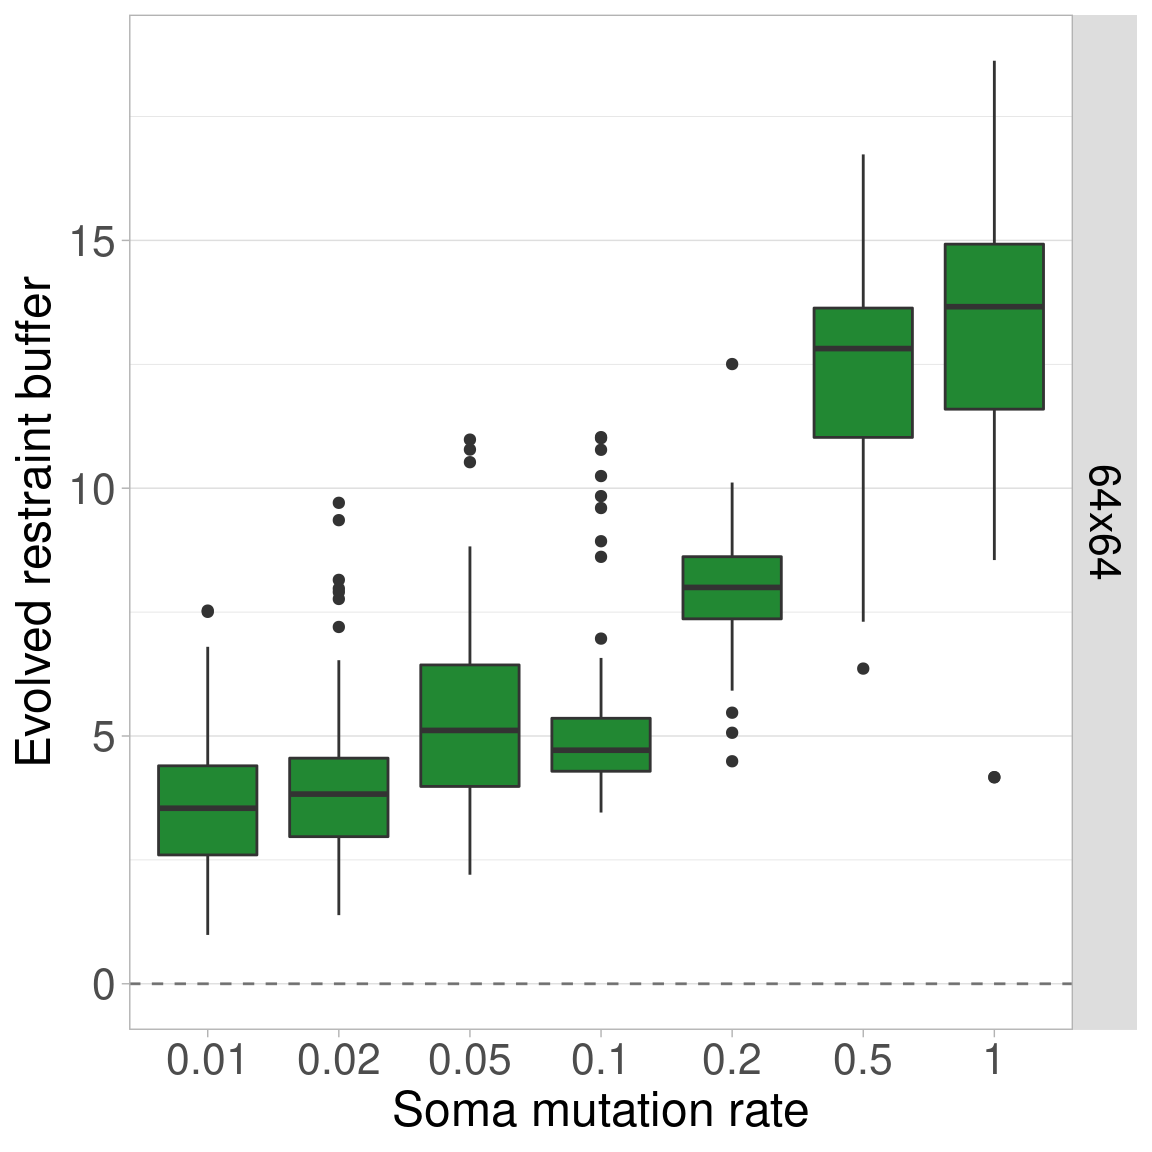
\includegraphics{primordium_supplemental_material_files/figure-latex/unnamed-chunk-21-1.pdf}

\hypertarget{organism-size-128x128}{%
\subsection{Organism size 128x128}\label{organism-size-128x128}}

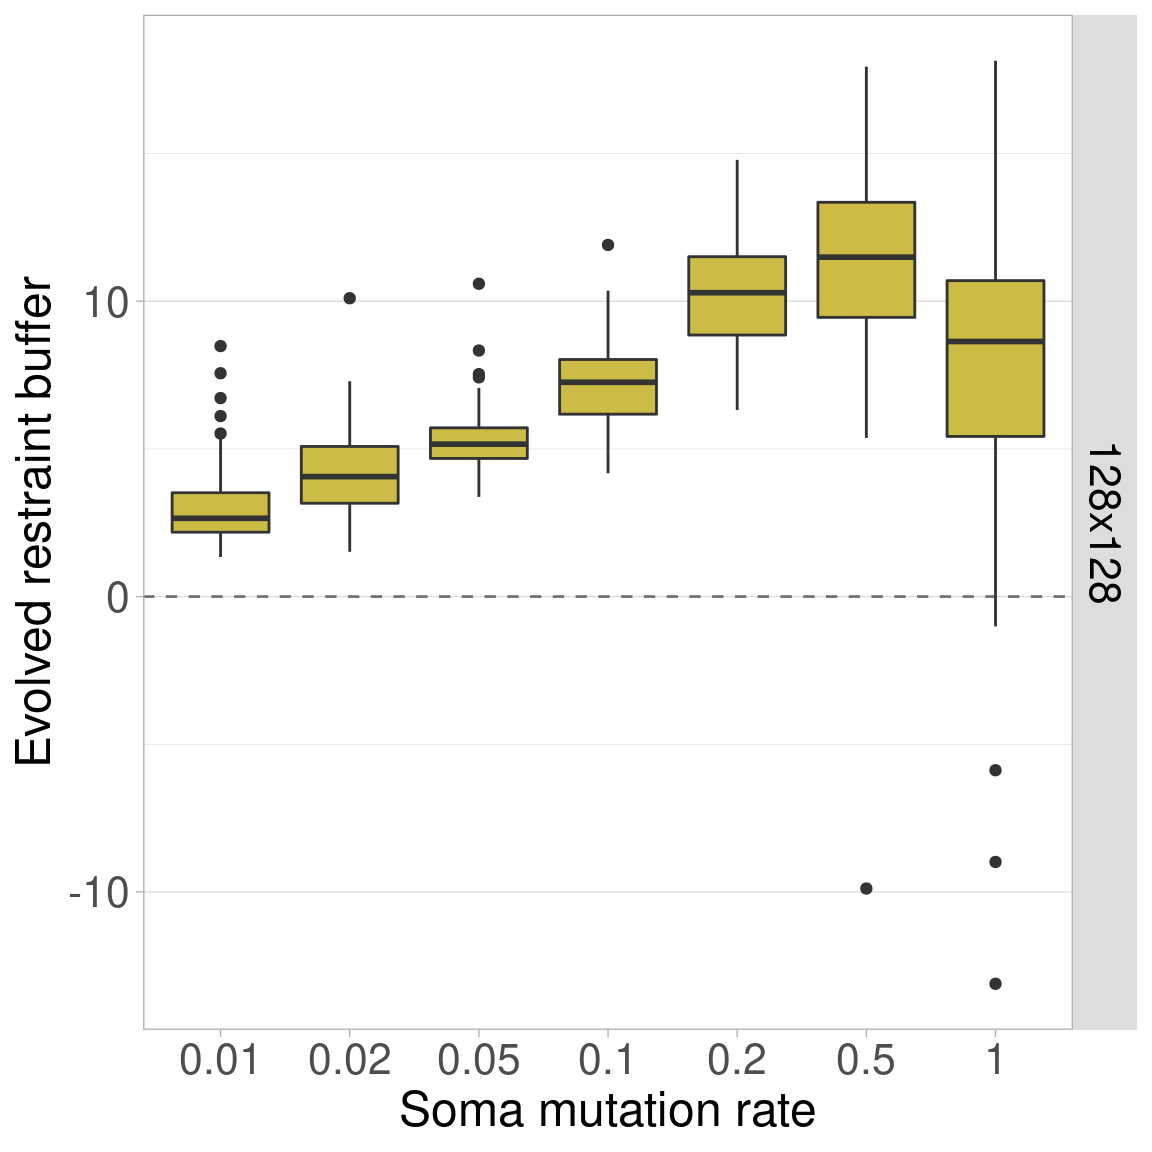
\includegraphics{primordium_supplemental_material_files/figure-latex/unnamed-chunk-22-1.pdf}

\hypertarget{organism-size-256x256}{%
\subsection{Organism size 256x256}\label{organism-size-256x256}}

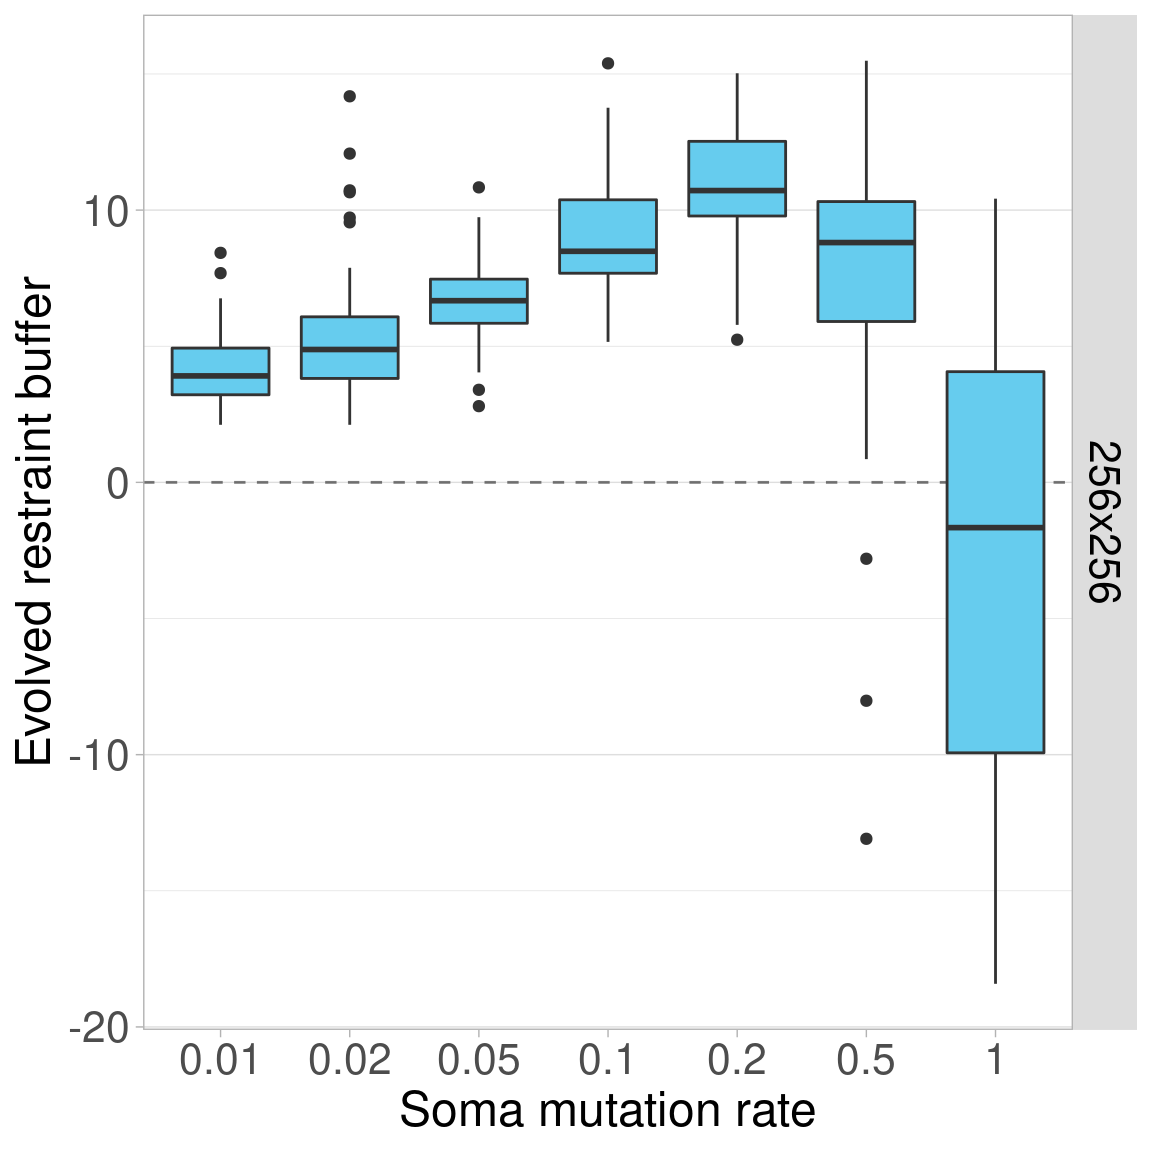
\includegraphics{primordium_supplemental_material_files/figure-latex/unnamed-chunk-23-1.pdf}

\hypertarget{organism-size-512x512}{%
\subsection{Organism size 512x512}\label{organism-size-512x512}}

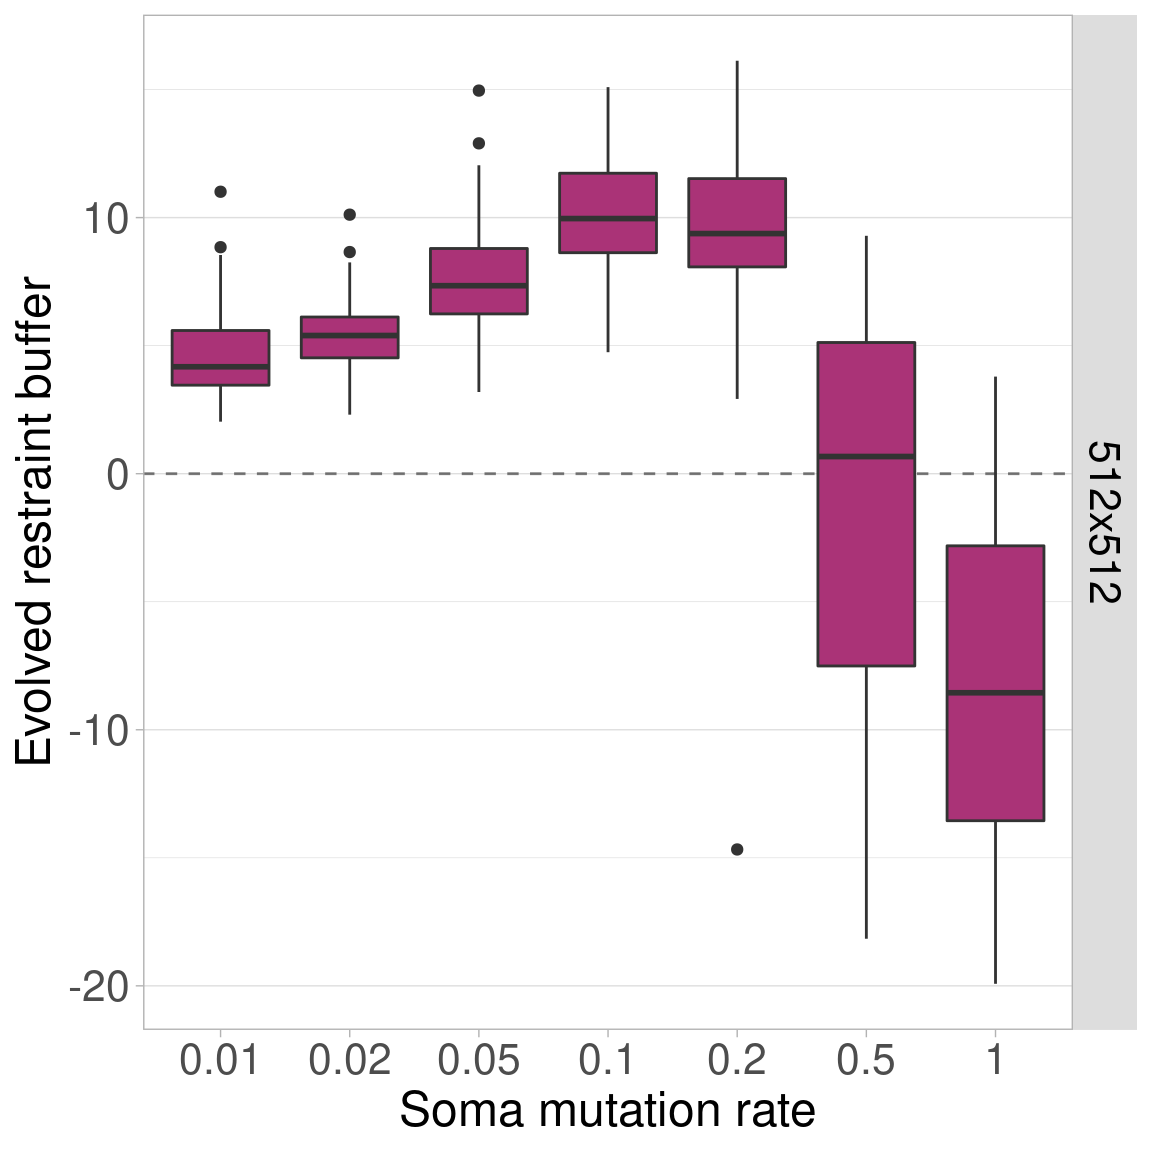
\includegraphics{primordium_supplemental_material_files/figure-latex/unnamed-chunk-24-1.pdf}

\hypertarget{single-somatic-mutation-rate-plots}{%
\section{Single somatic mutation rate plots}\label{single-somatic-mutation-rate-plots}}

Here we plot each somatic mutation rate independently, with organism size varying on the x-axis.

\hypertarget{somatic-mut.-rate-0.01}{%
\subsection{Somatic mut. rate 0.01}\label{somatic-mut.-rate-0.01}}

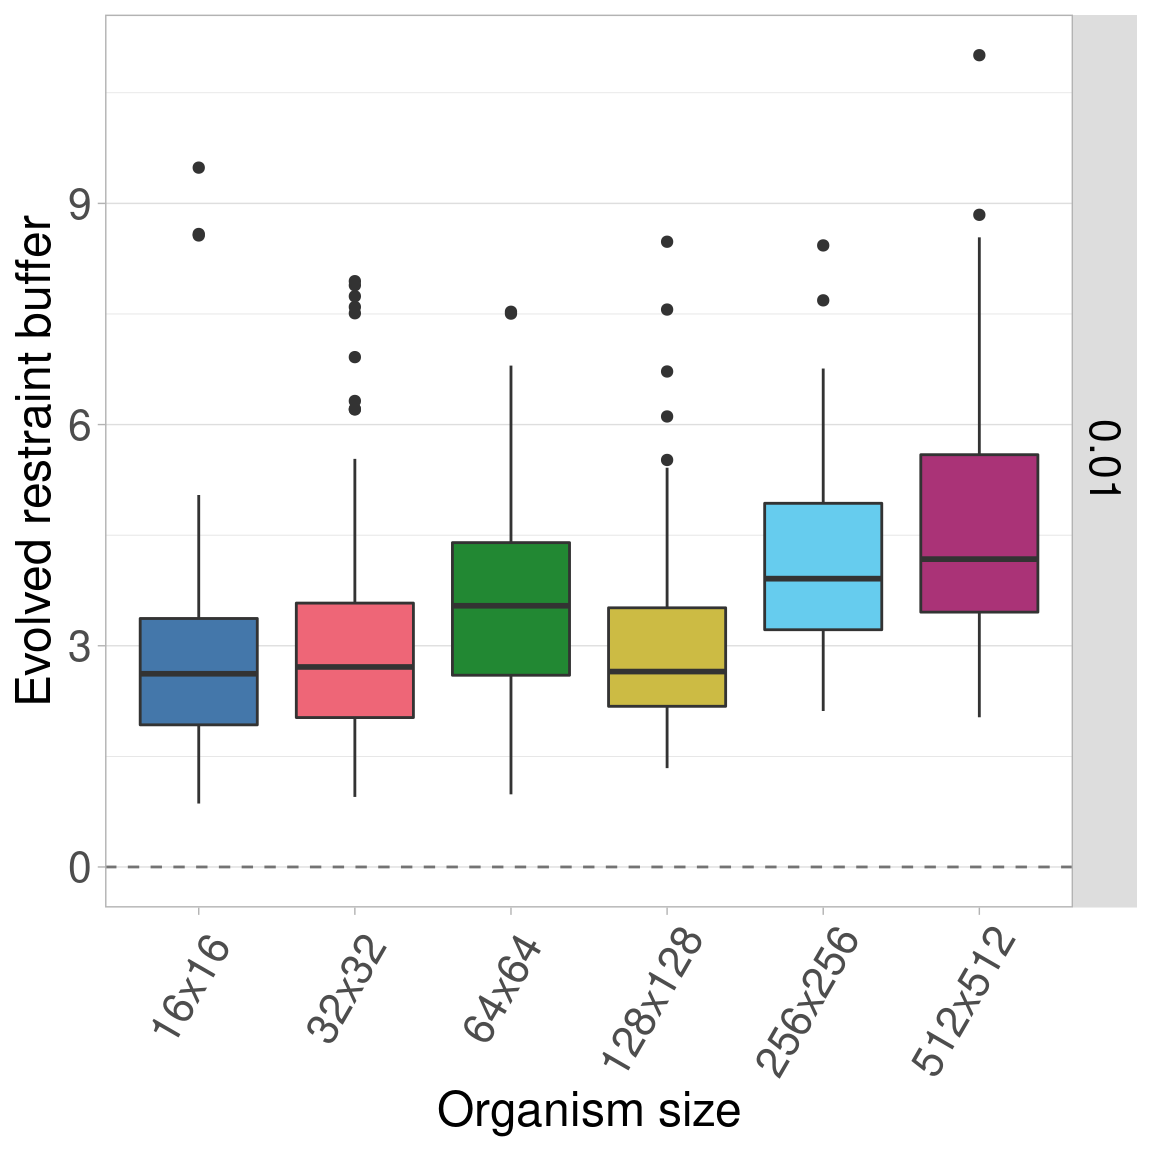
\includegraphics{primordium_supplemental_material_files/figure-latex/unnamed-chunk-25-1.pdf}

\hypertarget{somatic-mut.-rate-0.02}{%
\subsection{Somatic mut. rate 0.02}\label{somatic-mut.-rate-0.02}}

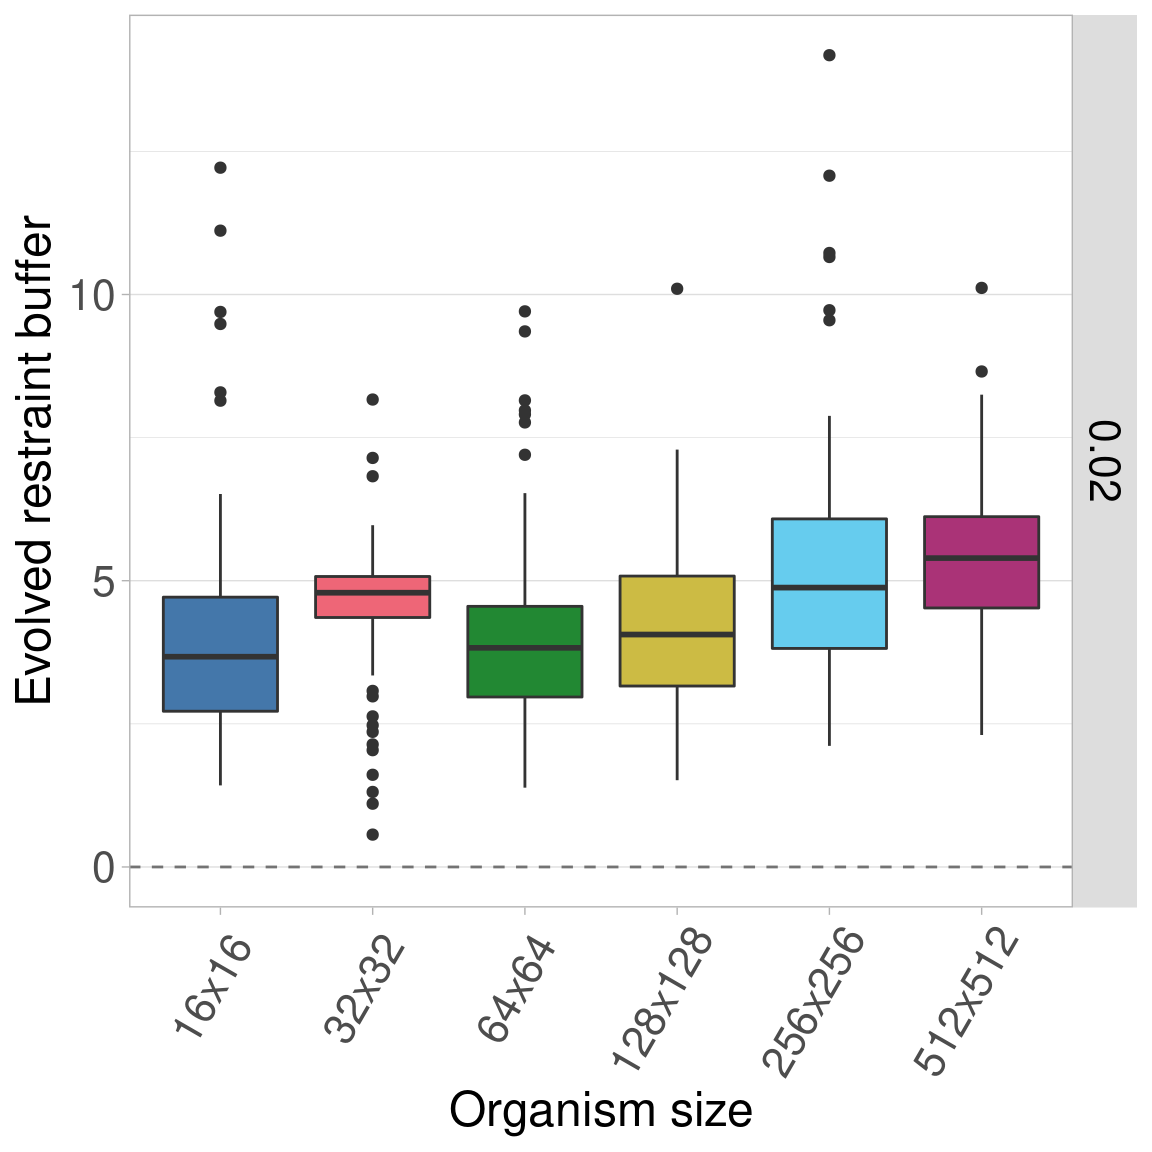
\includegraphics{primordium_supplemental_material_files/figure-latex/unnamed-chunk-26-1.pdf}

\hypertarget{somatic-mut.-rate-0.05}{%
\subsection{Somatic mut. rate 0.05}\label{somatic-mut.-rate-0.05}}

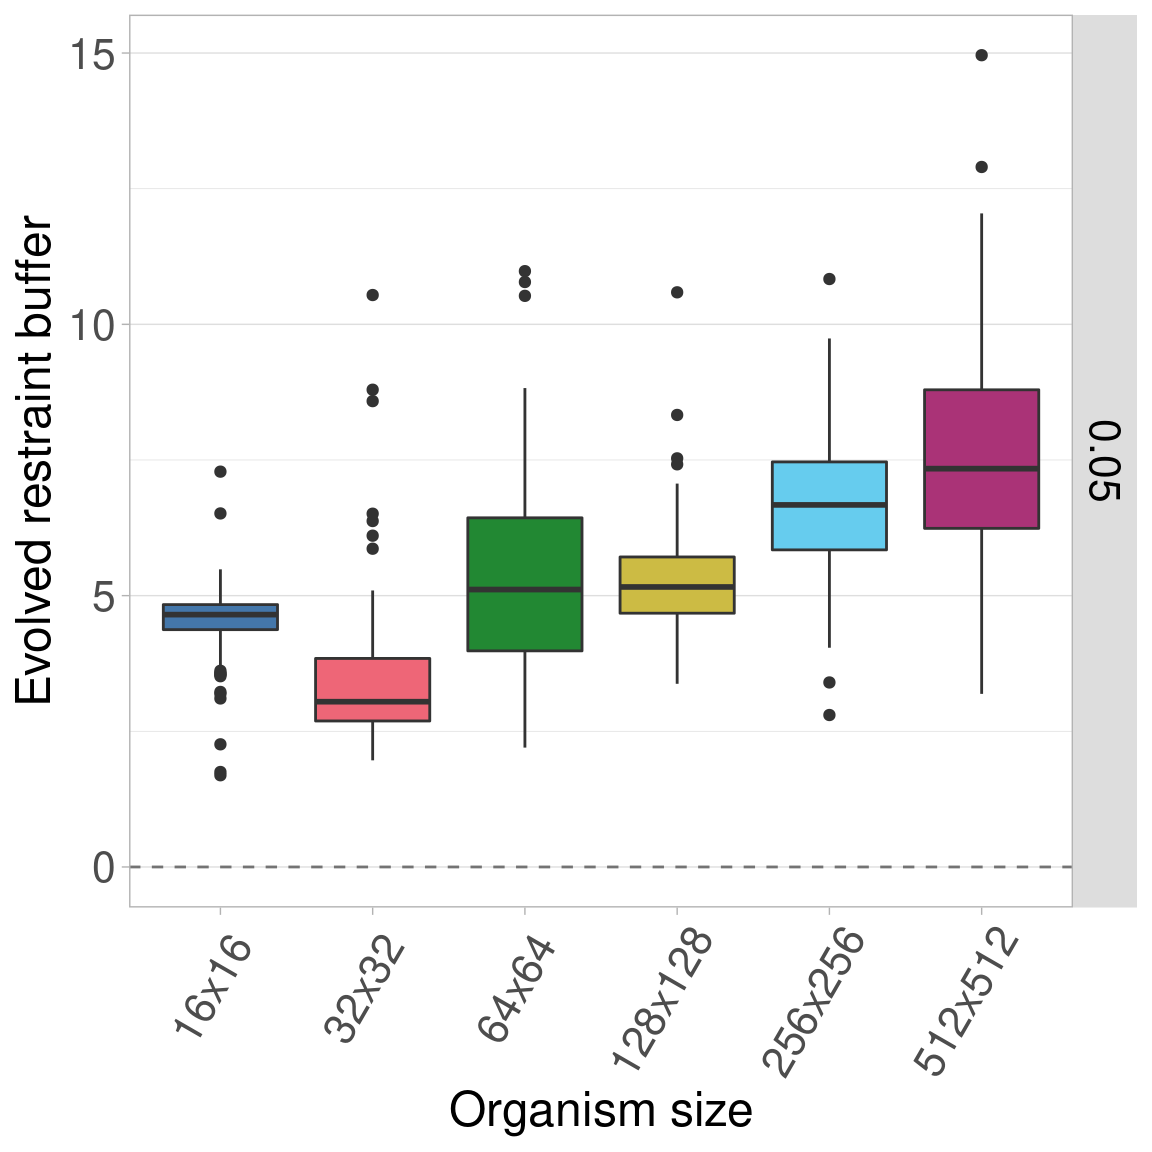
\includegraphics{primordium_supplemental_material_files/figure-latex/unnamed-chunk-27-1.pdf}

\hypertarget{somatic-mut.-rate-0.1}{%
\subsection{Somatic mut. rate 0.1}\label{somatic-mut.-rate-0.1}}

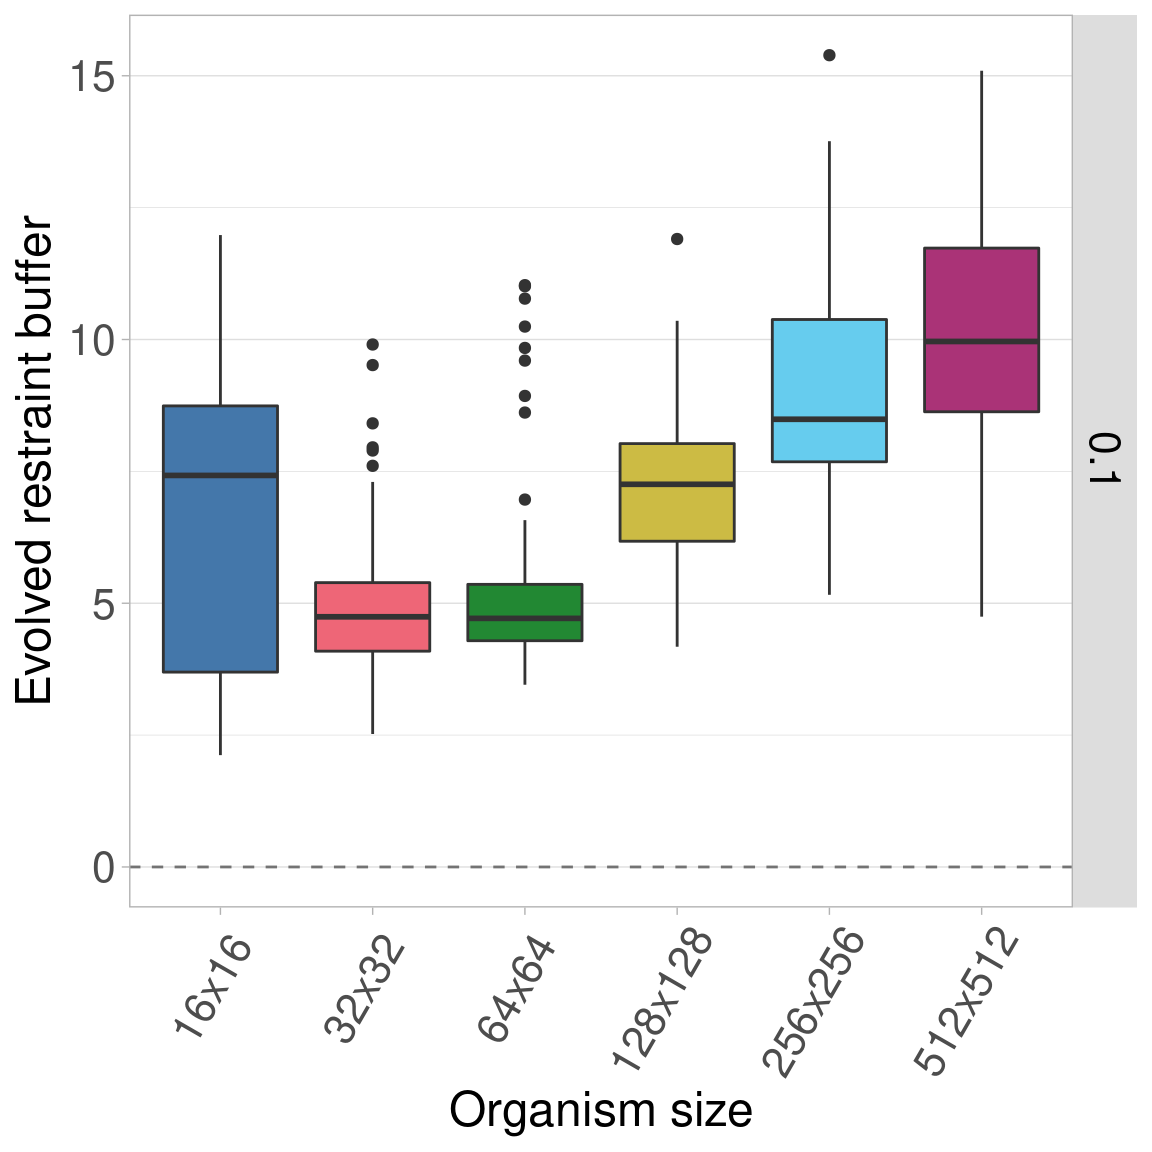
\includegraphics{primordium_supplemental_material_files/figure-latex/unnamed-chunk-28-1.pdf}

\hypertarget{somatic-mut.-rate-0.2}{%
\subsection{Somatic mut. rate 0.2}\label{somatic-mut.-rate-0.2}}

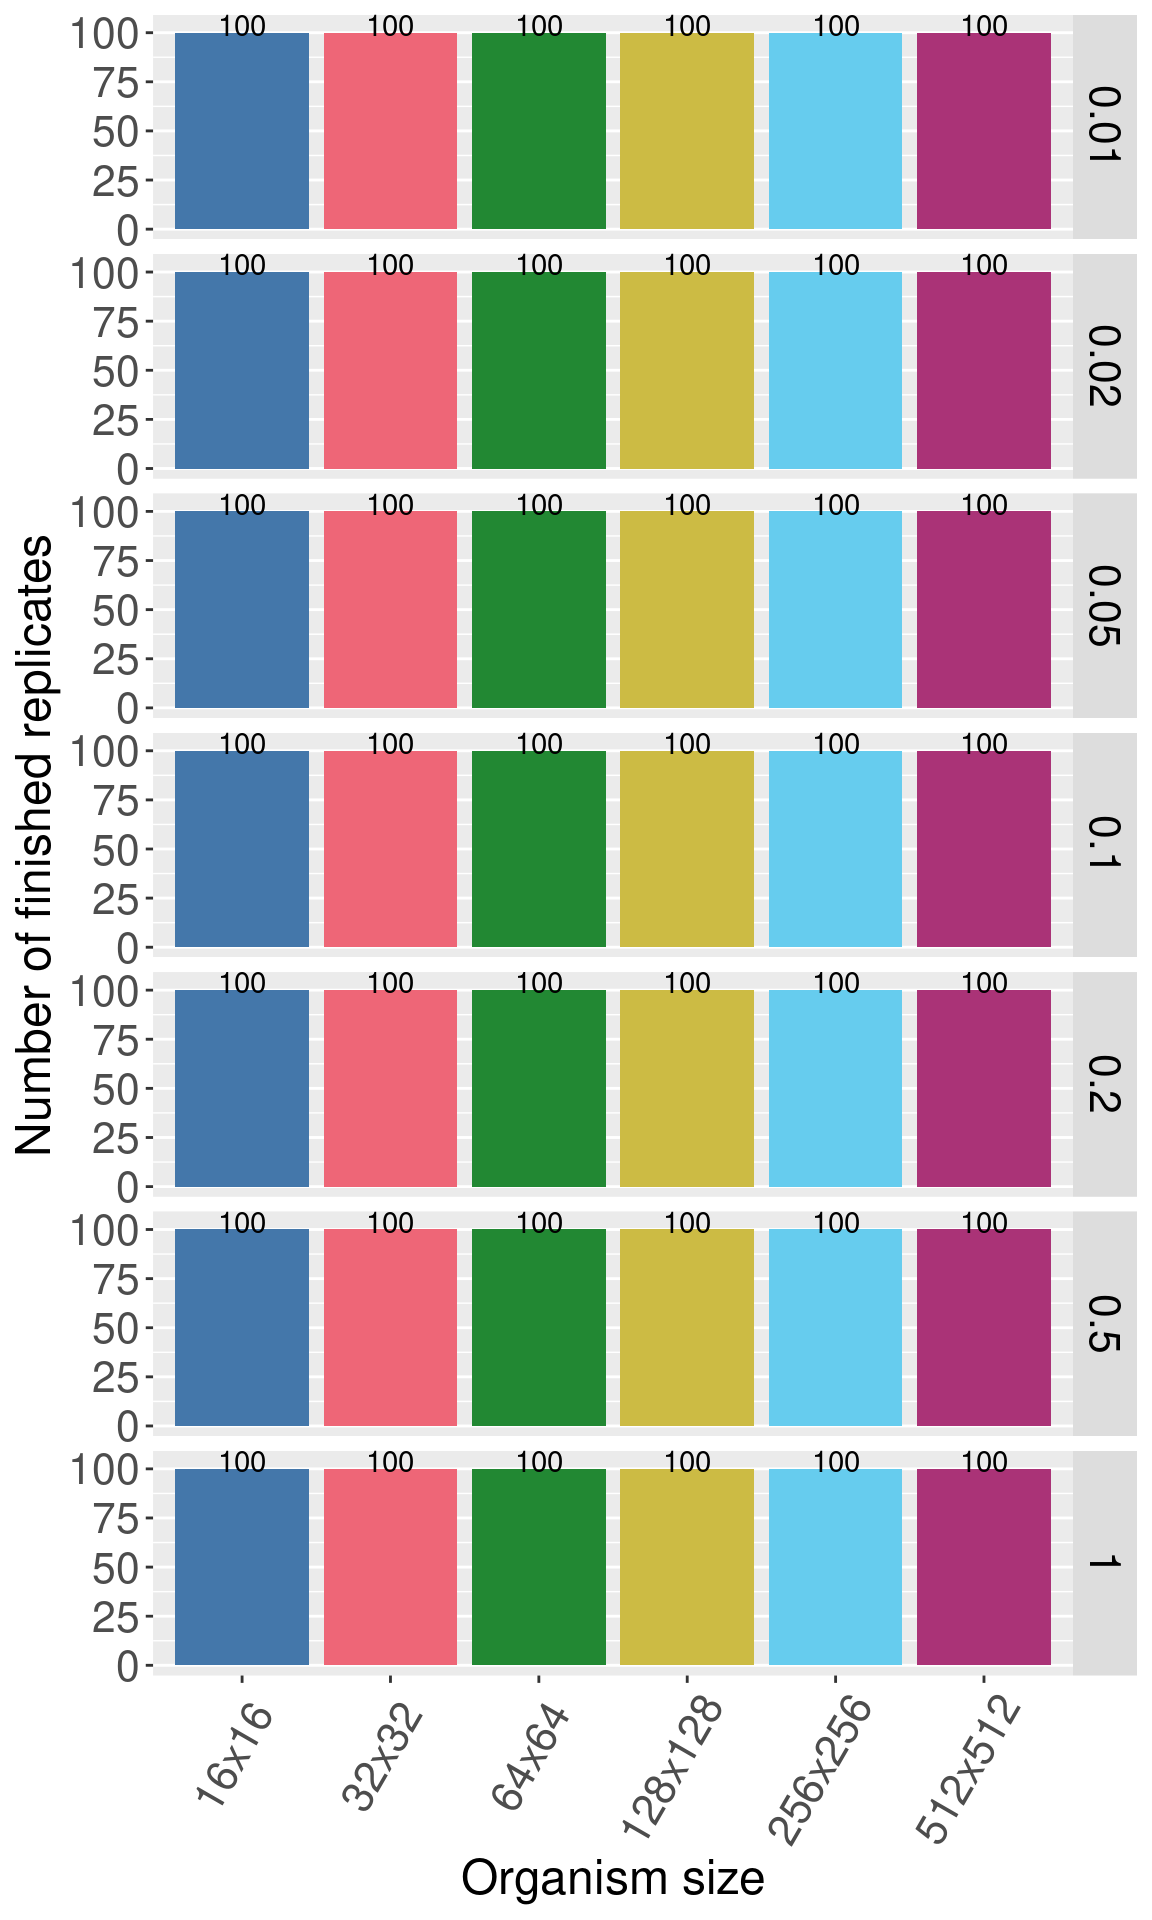
\includegraphics{primordium_supplemental_material_files/figure-latex/unnamed-chunk-29-1.pdf}

\hypertarget{somatic-mut.-rate-0.5}{%
\subsection{Somatic mut. rate 0.5}\label{somatic-mut.-rate-0.5}}

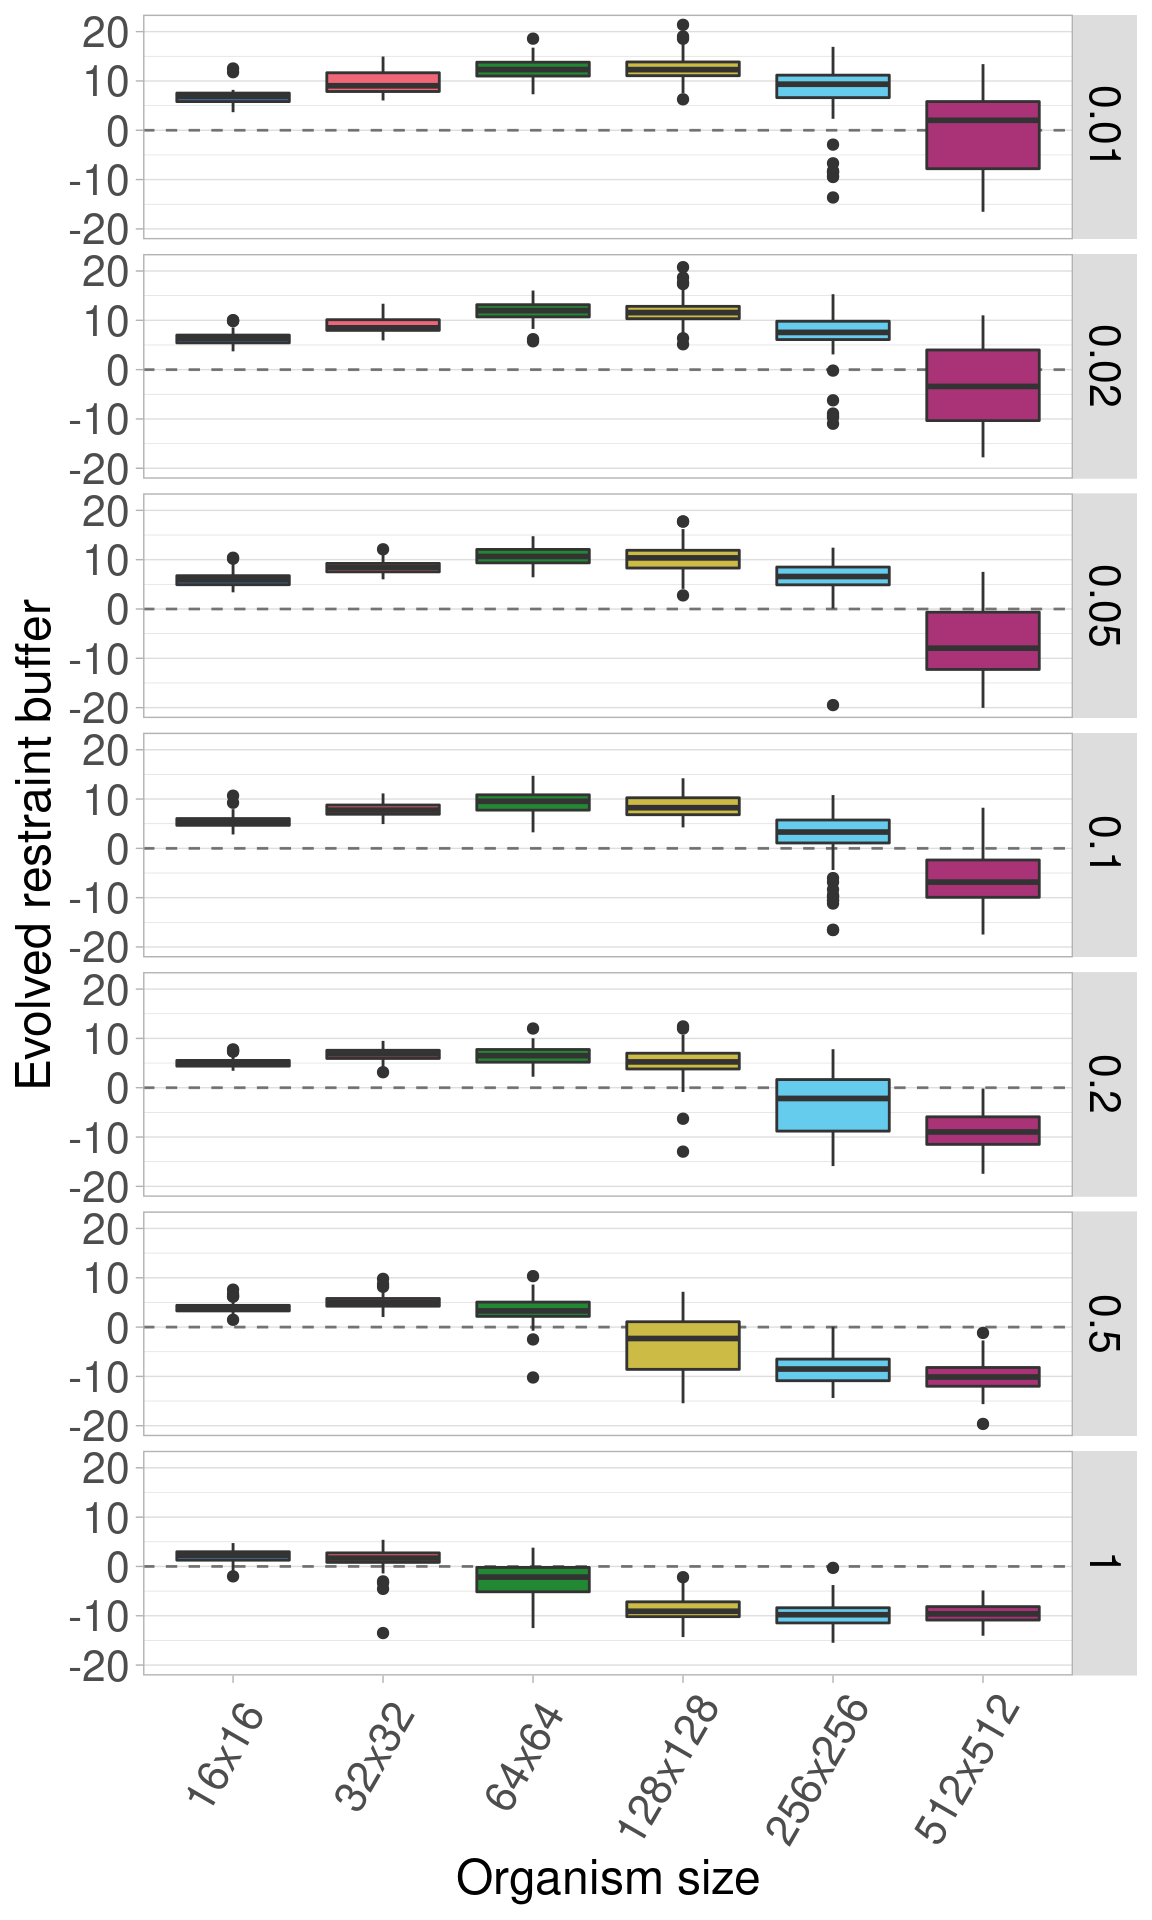
\includegraphics{primordium_supplemental_material_files/figure-latex/unnamed-chunk-30-1.pdf}

\hypertarget{somatic-mut.-rate-1.0}{%
\subsection{Somatic mut. rate 1.0}\label{somatic-mut.-rate-1.0}}

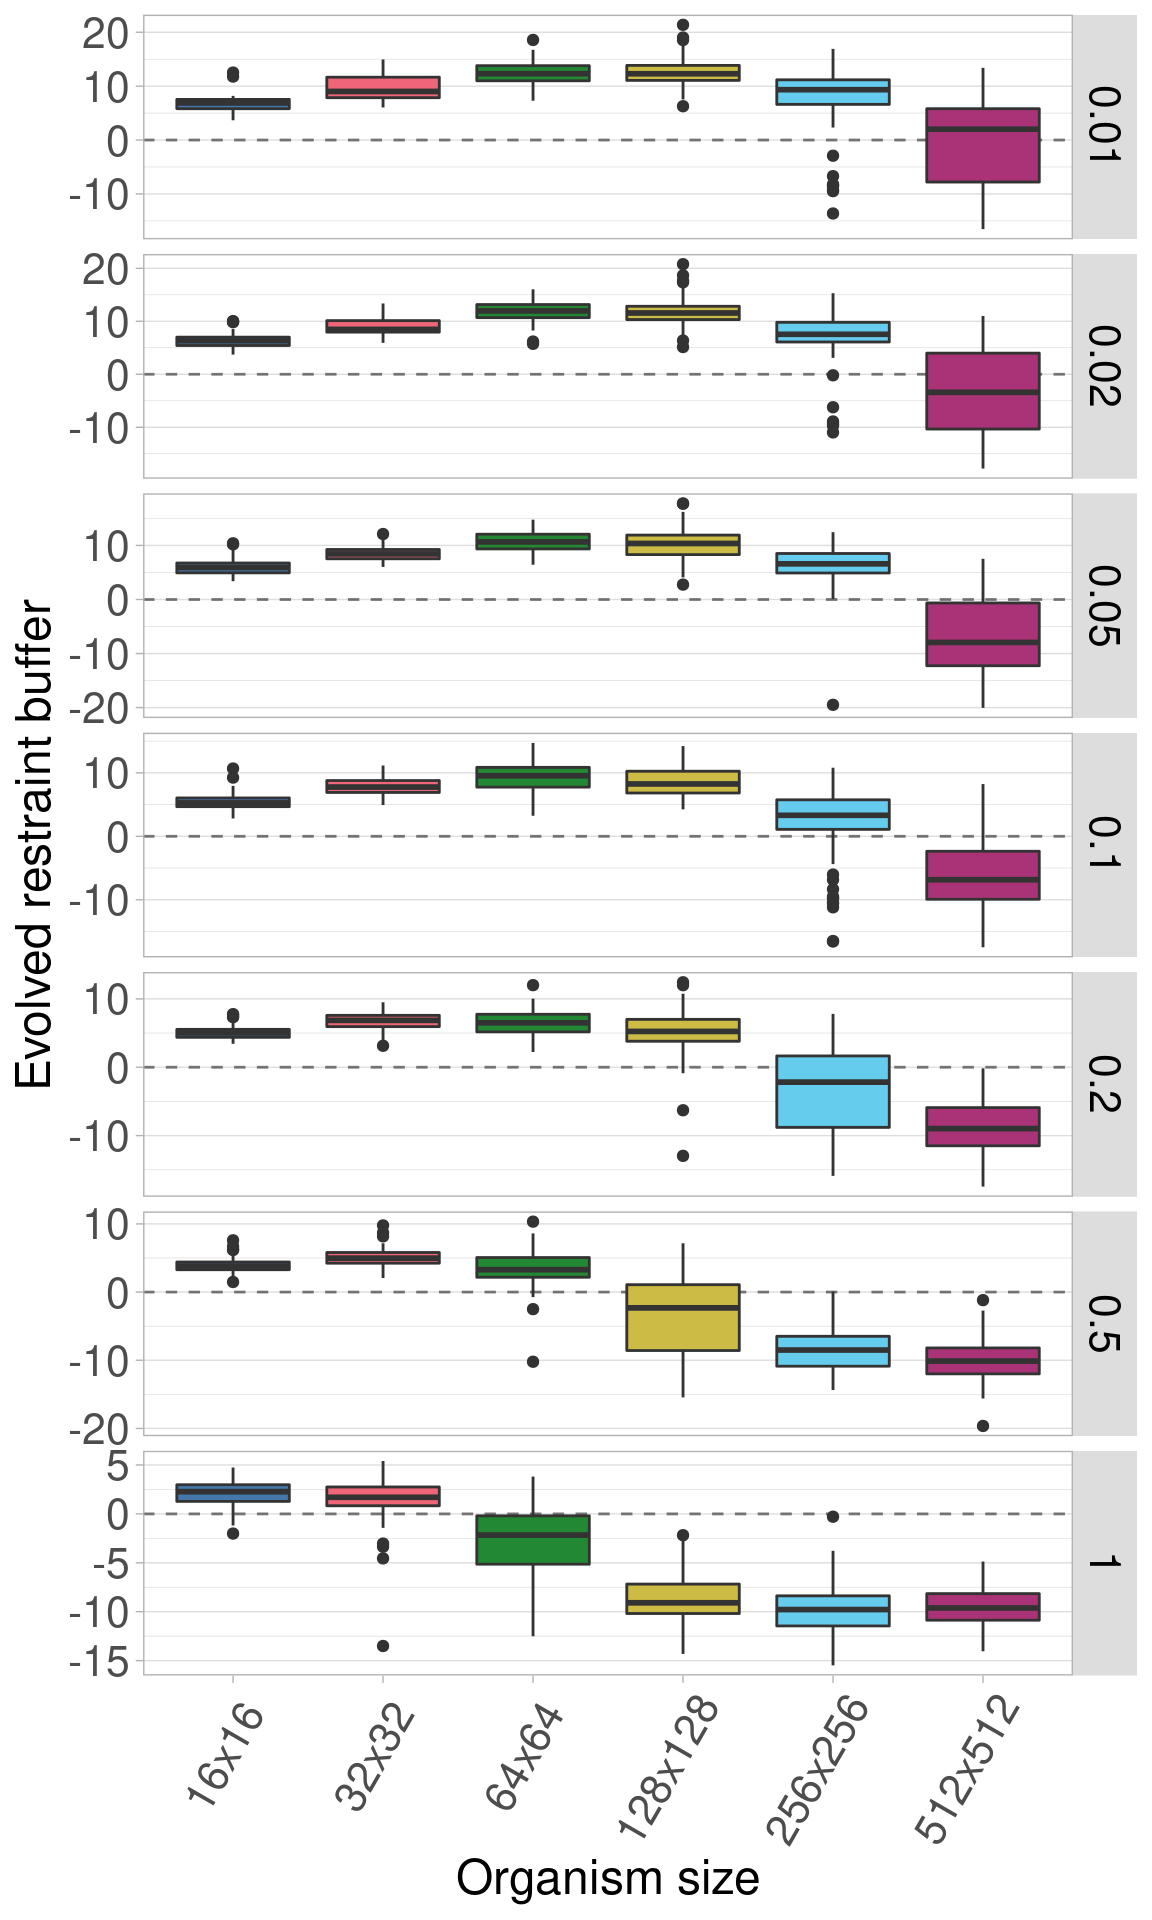
\includegraphics{primordium_supplemental_material_files/figure-latex/unnamed-chunk-31-1.pdf}

\hypertarget{statistics-1}{%
\section{Statistics}\label{statistics-1}}

Since organism size is our main point of comparison, we calculate statistics for each somatic mutation rate.

First, we perform a Kruskal-Wallis test across all organism sizes to indicate if variance exists at that mutation rate.
If variance exists, we then perform a pairwise Wilcoxon Rank-Sum test to show which pairs of organism sizes significantly differ.
Finally, we perform Bonferroni-Holm corrections for multiple comparisons.

\begin{Shaded}
\begin{Highlighting}[]
\NormalTok{  mut\_vec =}\StringTok{ }\KeywordTok{c}\NormalTok{(}\FloatTok{0.01}\NormalTok{, }\FloatTok{0.02}\NormalTok{, }\FloatTok{0.05}\NormalTok{, }\FloatTok{0.1}\NormalTok{, }\FloatTok{0.2}\NormalTok{, }\FloatTok{0.5}\NormalTok{, }\DecValTok{1}\NormalTok{)}
\NormalTok{  df\_kruskal =}\StringTok{ }\KeywordTok{data.frame}\NormalTok{(}\DataTypeTok{data =} \KeywordTok{matrix}\NormalTok{(}\DataTypeTok{nrow =} \DecValTok{0}\NormalTok{, }\DataTypeTok{ncol =} \DecValTok{4}\NormalTok{))}
  \KeywordTok{colnames}\NormalTok{(df\_kruskal) =}\StringTok{ }\KeywordTok{c}\NormalTok{(}\StringTok{\textquotesingle{}soma\_mut\_rate\textquotesingle{}}\NormalTok{, }\StringTok{\textquotesingle{}p\_value\textquotesingle{}}\NormalTok{, }\StringTok{\textquotesingle{}chi\_squared\textquotesingle{}}\NormalTok{, }\StringTok{\textquotesingle{}df\textquotesingle{}}\NormalTok{)}
  \ControlFlowTok{for}\NormalTok{(mut\_rate }\ControlFlowTok{in}\NormalTok{ mut\_vec)\{}
\NormalTok{    df\_test =}\StringTok{ }\NormalTok{df2[df2}\OperatorTok{$}\NormalTok{CELLMUT }\OperatorTok{==}\StringTok{ }\NormalTok{mut\_rate,]}
\NormalTok{    res =}\StringTok{ }\KeywordTok{kruskal.test}\NormalTok{(df\_test}\OperatorTok{$}\NormalTok{restraint\_value }\OperatorTok{\textasciitilde{}}\StringTok{ }\NormalTok{df\_test}\OperatorTok{$}\NormalTok{MCSIZE, df\_test)}
\NormalTok{    df\_kruskal[}\KeywordTok{nrow}\NormalTok{(df\_kruskal) }\OperatorTok{+}\StringTok{ }\DecValTok{1}\NormalTok{,] =}\StringTok{ }\KeywordTok{c}\NormalTok{(mut\_rate, res}\OperatorTok{$}\NormalTok{p.value, }\KeywordTok{as.numeric}\NormalTok{(res}\OperatorTok{$}\NormalTok{statistic)[}\DecValTok{1}\NormalTok{], }\KeywordTok{as.numeric}\NormalTok{(res}\OperatorTok{$}\NormalTok{parameter)[}\DecValTok{1}\NormalTok{])}
\NormalTok{  \}}
\NormalTok{  df\_kruskal}\OperatorTok{$}\NormalTok{less\_}\FloatTok{0.01}\NormalTok{ =}\StringTok{ }\NormalTok{df\_kruskal}\OperatorTok{$}\NormalTok{p\_value }\OperatorTok{\textless{}}\StringTok{ }\FloatTok{0.01}
  \KeywordTok{print}\NormalTok{(df\_kruskal)}
\end{Highlighting}
\end{Shaded}

\begin{verbatim}
##   soma_mut_rate      p_value chi_squared df less_0.01
## 1          0.01 2.661659e-25    125.0566  5      TRUE
## 2          0.02 4.808020e-19     95.4471  5      TRUE
## 3          0.05 1.142677e-63    304.3847  5      TRUE
## 4          0.10 3.945761e-64    306.5323  5      TRUE
## 5          0.20 4.924029e-79    375.7743  5      TRUE
## 6          0.50 5.011460e-85    403.5832  5      TRUE
## 7          1.00 5.474947e-99    468.3229  5      TRUE
\end{verbatim}

We see that significant variation exists within each mutation rate, so we perform pairwise Wilcoxon tests on each to see which pairs of sizes are significantly different.

\begin{Shaded}
\begin{Highlighting}[]
\NormalTok{size\_vec =}\StringTok{ }\KeywordTok{c}\NormalTok{(}\DecValTok{16}\NormalTok{, }\DecValTok{32}\NormalTok{, }\DecValTok{64}\NormalTok{, }\DecValTok{128}\NormalTok{, }\DecValTok{256}\NormalTok{, }\DecValTok{512}\NormalTok{)}
\NormalTok{mut\_vec =}\StringTok{ }\KeywordTok{c}\NormalTok{(}\FloatTok{0.01}\NormalTok{, }\FloatTok{0.02}\NormalTok{, }\FloatTok{0.05}\NormalTok{, }\FloatTok{0.1}\NormalTok{, }\FloatTok{0.2}\NormalTok{, }\FloatTok{0.5}\NormalTok{, }\DecValTok{1}\NormalTok{)}
\ControlFlowTok{for}\NormalTok{(mut\_rate }\ControlFlowTok{in}\NormalTok{ mut\_vec)\{}
\NormalTok{  df\_test =}\StringTok{ }\NormalTok{df2[df2}\OperatorTok{$}\NormalTok{CELLMUT }\OperatorTok{==}\StringTok{ }\NormalTok{mut\_rate,]}
\NormalTok{  df\_wilcox =}\StringTok{ }\KeywordTok{data.frame}\NormalTok{(}\DataTypeTok{data =} \KeywordTok{matrix}\NormalTok{(}\DataTypeTok{nrow =} \DecValTok{0}\NormalTok{, }\DataTypeTok{ncol =} \DecValTok{6}\NormalTok{))}
  \KeywordTok{colnames}\NormalTok{(df\_wilcox) =}\StringTok{ }\KeywordTok{c}\NormalTok{(}\StringTok{\textquotesingle{}mut\_rate\textquotesingle{}}\NormalTok{, }\StringTok{\textquotesingle{}size\_a\textquotesingle{}}\NormalTok{, }\StringTok{\textquotesingle{}size\_b\textquotesingle{}}\NormalTok{, }\StringTok{\textquotesingle{}p\_value\_corrected\textquotesingle{}}\NormalTok{, }\StringTok{\textquotesingle{}p\_value\_raw\textquotesingle{}}\NormalTok{, }\StringTok{\textquotesingle{}W\textquotesingle{}}\NormalTok{)}
  \ControlFlowTok{for}\NormalTok{(size\_idx\_a }\ControlFlowTok{in} \DecValTok{1}\OperatorTok{:}\NormalTok{(}\KeywordTok{length}\NormalTok{(size\_vec) }\OperatorTok{{-}}\StringTok{ }\DecValTok{1}\NormalTok{))\{}
\NormalTok{    size\_a =}\StringTok{ }\NormalTok{size\_vec[size\_idx\_a]}
    \ControlFlowTok{for}\NormalTok{(size\_idx\_b }\ControlFlowTok{in}\NormalTok{ (size\_idx\_a }\OperatorTok{+}\StringTok{ }\DecValTok{1}\NormalTok{)}\OperatorTok{:}\KeywordTok{length}\NormalTok{(size\_vec))\{}
\NormalTok{      size\_b =}\StringTok{ }\NormalTok{size\_vec[size\_idx\_b]}
\NormalTok{      res =}\StringTok{ }\KeywordTok{wilcox.test}\NormalTok{(df\_test[df\_test}\OperatorTok{$}\NormalTok{MCSIZE }\OperatorTok{==}\StringTok{ }\NormalTok{size\_a,]}\OperatorTok{$}\NormalTok{restraint\_value, df\_test[df\_test}\OperatorTok{$}\NormalTok{MCSIZE }\OperatorTok{==}\StringTok{ }\NormalTok{size\_b,]}\OperatorTok{$}\NormalTok{restraint\_value, }\DataTypeTok{alternative =} \StringTok{\textquotesingle{}two.sided\textquotesingle{}}\NormalTok{) }
\NormalTok{      df\_wilcox[}\KeywordTok{nrow}\NormalTok{(df\_wilcox) }\OperatorTok{+}\StringTok{ }\DecValTok{1}\NormalTok{,] =}\StringTok{ }\KeywordTok{c}\NormalTok{(mut\_rate, size\_a, size\_b, }\DecValTok{0}\NormalTok{, res}\OperatorTok{$}\NormalTok{p.value, }\KeywordTok{as.numeric}\NormalTok{(res}\OperatorTok{$}\NormalTok{statistic)[}\DecValTok{1}\NormalTok{])}
\NormalTok{    \}}
\NormalTok{  \}}
\NormalTok{  df\_wilcox}\OperatorTok{$}\NormalTok{p\_value\_corrected =}\StringTok{ }\KeywordTok{p.adjust}\NormalTok{(df\_wilcox}\OperatorTok{$}\NormalTok{p\_value\_raw, }\DataTypeTok{method =} \StringTok{\textquotesingle{}holm\textquotesingle{}}\NormalTok{)}
\NormalTok{  df\_wilcox}\OperatorTok{$}\NormalTok{less\_}\FloatTok{0.01}\NormalTok{ =}\StringTok{ }\NormalTok{df\_wilcox}\OperatorTok{$}\NormalTok{p\_value\_corrected }\OperatorTok{\textless{}}\StringTok{ }\FloatTok{0.01}
  \KeywordTok{print}\NormalTok{(}\KeywordTok{paste0}\NormalTok{(}\StringTok{\textquotesingle{}Somatic mutation rate: \textquotesingle{}}\NormalTok{, mut\_rate))}
  \KeywordTok{print}\NormalTok{(df\_wilcox)}
\NormalTok{\}}
\end{Highlighting}
\end{Shaded}

\begin{verbatim}
## [1] "Somatic mutation rate: 0.01"
##    mut_rate size_a size_b p_value_corrected  p_value_raw      W less_0.01
## 1      0.01     16     32      9.390497e-01 4.695249e-01 4703.5     FALSE
## 2      0.01     16     64      2.988154e-04 3.735192e-05 3312.0      TRUE
## 3      0.01     16    128      7.079843e-01 2.359948e-01 4514.5     FALSE
## 4      0.01     16    256      2.034819e-12 1.453442e-13 1974.5      TRUE
## 5      0.01     16    512      4.368517e-15 2.912344e-16 1653.0      TRUE
## 6      0.01     32     64      1.074876e-02 1.535537e-03 3703.0     FALSE
## 7      0.01     32    128      9.390497e-01 7.176323e-01 4851.5     FALSE
## 8      0.01     32    256      8.111610e-09 8.111610e-10 2485.5      TRUE
## 9      0.01     32    512      1.748038e-11 1.456698e-12 2102.5      TRUE
## 10     0.01     64    128      1.074876e-02 1.601365e-03 6292.0     FALSE
## 11     0.01     64    256      1.397091e-02 2.794183e-03 3776.0     FALSE
## 12     0.01     64    512      7.748038e-05 8.608931e-06 3178.5      TRUE
## 13     0.01    128    256      3.676583e-09 3.342348e-10 2428.5      TRUE
## 14     0.01    128    512      2.110112e-12 1.623163e-13 1980.5      TRUE
## 15     0.01    256    512      2.266729e-01 5.666822e-02 4219.5     FALSE
## [1] "Somatic mutation rate: 0.02"
##    mut_rate size_a size_b p_value_corrected  p_value_raw      W less_0.01
## 1      0.02     16     32      3.611494e-05 4.012771e-06 3112.5      TRUE
## 2      0.02     16     64      4.740405e-01 4.740405e-01 4706.5     FALSE
## 3      0.02     16    128      2.648393e-01 5.296786e-02 4207.5     FALSE
## 4      0.02     16    256      6.698428e-07 5.582024e-08 2776.5      TRUE
## 5      0.02     16    512      4.142268e-11 2.761512e-12 2139.0      TRUE
## 6      0.02     32     64      1.240992e-05 1.240992e-06 6985.0      TRUE
## 7      0.02     32    128      2.150816e-02 3.584693e-03 6192.5     FALSE
## 8      0.02     32    256      3.993493e-01 9.983733e-02 4326.0     FALSE
## 9      0.02     32    512      1.117168e-04 1.396459e-05 3221.5      TRUE
## 10     0.02     64    128      4.025666e-01 2.012833e-01 4476.5     FALSE
## 11     0.02     64    256      5.648464e-06 5.134967e-07 2944.5      TRUE
## 12     0.02     64    512      6.120346e-11 4.371676e-12 2165.5      TRUE
## 13     0.02    128    256      3.129242e-04 4.470345e-05 3329.0      TRUE
## 14     0.02    128    512      1.760116e-08 1.353935e-09 2519.0      TRUE
## 15     0.02    256    512      3.993493e-01 1.013587e-01 4329.0     FALSE
## [1] "Somatic mutation rate: 0.05"
##    mut_rate size_a size_b p_value_corrected  p_value_raw      W less_0.01
## 1      0.05     16     32      8.163575e-15 9.070638e-16 8290.5      TRUE
## 2      0.05     16     64      1.254683e-03 4.182276e-04 3555.5      TRUE
## 3      0.05     16    128      2.819711e-09 5.639421e-10 2462.0      TRUE
## 4      0.05     16    256      1.007639e-23 8.396990e-25  791.0      TRUE
## 5      0.05     16    512      3.169326e-24 2.437943e-25  742.5      TRUE
## 6      0.05     32     64      9.865308e-14 1.409330e-14 1850.0      TRUE
## 7      0.05     32    128      9.672216e-22 8.792924e-23  978.5      TRUE
## 8      0.05     32    256      4.456762e-26 3.183402e-27  576.5      TRUE
## 9      0.05     32    512      1.225797e-27 8.171978e-29  441.0      TRUE
## 10     0.05     64    128      9.619980e-01 9.619980e-01 4980.0     FALSE
## 11     0.05     64    256      4.409184e-09 1.102296e-09 2505.5      TRUE
## 12     0.05     64    512      1.967988e-13 3.279979e-14 1894.5      TRUE
## 13     0.05    128    256      3.061979e-14 3.827473e-15 1782.5      TRUE
## 14     0.05    128    512      4.080298e-17 4.080298e-18 1448.5      TRUE
## 15     0.05    256    512      2.648877e-03 1.324439e-03 3685.5      TRUE
## [1] "Somatic mutation rate: 0.1"
##    mut_rate size_a size_b p_value_corrected  p_value_raw      W less_0.01
## 1       0.1     16     32      3.903716e-03 9.759291e-04 6350.0      TRUE
## 2       0.1     16     64      9.815188e-02 3.271729e-02 5874.5     FALSE
## 3       0.1     16    128      6.061146e-01 3.140880e-01 4587.5     FALSE
## 4       0.1     16    256      3.278276e-08 5.463793e-09 2612.5      TRUE
## 5       0.1     16    512      9.506115e-18 1.188264e-18 1391.5      TRUE
## 6       0.1     32     64      6.061146e-01 3.030573e-01 4578.0     FALSE
## 7       0.1     32    128      8.673971e-21 8.673971e-22 1074.0      TRUE
## 8       0.1     32    256      6.950798e-29 4.964856e-30  340.0      TRUE
## 9       0.1     32    512      1.934395e-30 1.289597e-31  211.5      TRUE
## 10      0.1     64    128      2.239733e-18 2.488592e-19 1320.5      TRUE
## 11      0.1     64    256      1.194130e-25 9.951080e-27  619.5      TRUE
## 12      0.1     64    512      1.966283e-27 1.512525e-28  463.5      TRUE
## 13      0.1    128    256      8.038941e-11 1.148420e-11 2222.0      TRUE
## 14      0.1    128    512      1.880691e-21 1.709719e-22 1006.0      TRUE
## 15      0.1    256    512      3.931365e-04 7.862729e-05 3383.5      TRUE
## [1] "Somatic mutation rate: 0.2"
##    mut_rate size_a size_b p_value_corrected  p_value_raw      W less_0.01
## 1       0.2     16     32      1.077048e-02 5.385238e-03 3860.5     FALSE
## 2       0.2     16     64      6.720281e-24 8.400351e-25  791.0      TRUE
## 3       0.2     16    128      1.215721e-28 1.013101e-29  365.5      TRUE
## 4       0.2     16    256      4.359012e-29 3.353086e-30  326.0      TRUE
## 5       0.2     16    512      3.611807e-25 3.283461e-26  665.0      TRUE
## 6       0.2     32     64      5.255254e-22 7.507505e-23  972.0      TRUE
## 7       0.2     32    128      3.542154e-29 2.530110e-30  316.0      TRUE
## 8       0.2     32    256      3.153758e-30 2.102505e-31  228.5      TRUE
## 9       0.2     32    512      1.346976e-24 1.496640e-25  723.5      TRUE
## 10      0.2     64    128      1.237545e-13 2.062574e-14 1870.0      TRUE
## 11      0.2     64    256      6.129521e-25 6.129521e-26  689.0      TRUE
## 12      0.2     64    512      1.436552e-07 2.873105e-08 2728.5      TRUE
## 13      0.2    128    256      6.935985e-03 2.311995e-03 3752.5      TRUE
## 14      0.2    128    512      1.987108e-01 1.987108e-01 5526.5     FALSE
## 15      0.2    256    512      3.309684e-04 8.274210e-05 6611.5      TRUE
## [1] "Somatic mutation rate: 0.5"
##    mut_rate size_a size_b p_value_corrected  p_value_raw      W less_0.01
## 1       0.5     16     32      1.212403e-25 1.212403e-26  627.0      TRUE
## 2       0.5     16     64      1.029212e-31 7.351512e-33  113.0      TRUE
## 3       0.5     16    128      1.432034e-27 1.301849e-28  458.0      TRUE
## 4       0.5     16    256      3.887685e-06 1.295895e-06 3018.5      TRUE
## 5       0.5     16    512      1.499786e-19 2.499644e-20 8781.5      TRUE
## 6       0.5     32     64      3.854284e-24 4.282538e-25  764.5      TRUE
## 7       0.5     32    128      6.344735e-14 1.268947e-14 1844.5      TRUE
## 8       0.5     32    256      6.346151e-01 6.346151e-01 5195.0     FALSE
## 9       0.5     32    512      3.036159e-31 2.335507e-32 9847.5      TRUE
## 10      0.5     64    128      9.397051e-03 4.698526e-03 6157.5      TRUE
## 11      0.5     64    256      6.907801e-20 9.868288e-21 8822.0      TRUE
## 12      0.5     64    512      9.160009e-33 6.106673e-34 9971.0      TRUE
## 13      0.5    128    256      4.999760e-11 1.249940e-11 7773.0      TRUE
## 14      0.5    128    512      6.054856e-31 5.045714e-32 9821.0      TRUE
## 15      0.5    256    512      4.216225e-21 5.270281e-22 8947.0      TRUE
## [1] "Somatic mutation rate: 1"
##    mut_rate size_a size_b p_value_corrected  p_value_raw       W less_0.01
## 1         1     16     32      2.812620e-27 3.515774e-28   494.5      TRUE
## 2         1     16     64      5.606003e-22 9.343338e-23   981.0      TRUE
## 3         1     16    128      2.202125e-02 1.101063e-02  6041.0     FALSE
## 4         1     16    256      4.073858e-28 4.526509e-29  9580.5      TRUE
## 5         1     16    512      3.841268e-33 2.561566e-34 10000.0      TRUE
## 6         1     32     64      7.619035e-01 7.619035e-01  5124.5     FALSE
## 7         1     32    128      2.931097e-22 4.187282e-23  9052.0      TRUE
## 8         1     32    256      3.841268e-33 2.976903e-34  9995.0      TRUE
## 9         1     32    512      3.841268e-33 2.561711e-34 10000.0      TRUE
## 10        1     64    128      1.456083e-19 3.640207e-20  8765.0      TRUE
## 11        1     64    256      2.413338e-32 2.193944e-33  9928.0      TRUE
## 12        1     64    512      3.841268e-33 2.560845e-34 10000.0      TRUE
## 13        1    128    256      1.180975e-20 2.361951e-21  8883.5      TRUE
## 14        1    128    512      1.253447e-30 1.253447e-31  9789.5      TRUE
## 15        1    256    512      6.072904e-07 2.024301e-07  7127.5      TRUE
\end{verbatim}

\hypertarget{germ-mutation-rate-sweep}{%
\chapter{Germ Mutation Rate Sweep}\label{germ-mutation-rate-sweep}}

This was one of the preliminary experiments we conducted to find the default parameters for Primordium.
However, the data shown here were ran after the system was finalized (with new random number seeds).
There were no qualitative differences from prior results.

We vary the \emph{germ} mutation rate, which is the probability that an offspring experiences a mutation to its restraint buffer during organism reproduction.
The probability of a mutation is per-genome, not per-bit.
When a germ mutation occurs, only a change of +/-1 is possible in the restraint buffer.
The final default germ mutation rate was 0.02 (\emph{i.e.}, each organism reproduction has a 2\% chance of mutation).

The configuration script and data for the experiment can be found under \texttt{2021\_02\_16\_\_germ\_mut\_fin/} in the experiments directory of the git repository.

\hypertarget{data-cleaning-2}{%
\section{Data cleaning}\label{data-cleaning-2}}

Load necessary R libraries

\begin{Shaded}
\begin{Highlighting}[]
\KeywordTok{library}\NormalTok{(dplyr)}
\KeywordTok{library}\NormalTok{(ggplot2)}
\KeywordTok{library}\NormalTok{(ggridges)}
\KeywordTok{library}\NormalTok{(scales)}
\KeywordTok{library}\NormalTok{(khroma)}
\end{Highlighting}
\end{Shaded}

Load the data and trim include only the final generation data for sizes 16x16 to 512x512.

\begin{Shaded}
\begin{Highlighting}[]
\CommentTok{\# Load the data}
\NormalTok{df =}\StringTok{ }\KeywordTok{read.csv}\NormalTok{(}\StringTok{\textquotesingle{}../experiments/2021\_02\_16\_\_germ\_mut\_fin/evolution/data/scraped\_evolution\_data.csv\textquotesingle{}}\NormalTok{)}
\CommentTok{\#df = read.csv(\textquotesingle{}/research/rogue\_cell/Primordium/experiments/2021\_02\_16\_\_germ\_mut\_fin/evolution/data/scraped\_evolution\_data.csv\textquotesingle{})}
\CommentTok{\# Trim off NAs (artifacts of how we scraped the data) and trim to only have gen 10,000}
\KeywordTok{cat}\NormalTok{(}\KeywordTok{colnames}\NormalTok{(df), }\StringTok{\textquotesingle{}}\CharTok{\textbackslash{}n}\StringTok{\textquotesingle{}}\NormalTok{)}
\end{Highlighting}
\end{Shaded}

\begin{verbatim}
## X generation ave_ones ave_repro_time min_ones max_ones var_ones rep_id MCSIZE COST GENS MUT POP SAMPLES REPS ONES CELLMUT
\end{verbatim}

\begin{Shaded}
\begin{Highlighting}[]
\NormalTok{df2 =}\StringTok{ }\NormalTok{df[}\OperatorTok{!}\KeywordTok{is.na}\NormalTok{(df}\OperatorTok{$}\NormalTok{MCSIZE) }\OperatorTok{\&}\StringTok{ }\NormalTok{df}\OperatorTok{$}\NormalTok{generation }\OperatorTok{==}\StringTok{ }\DecValTok{10000}\NormalTok{,]}
\CommentTok{\# Ignore data for size 8x8 and 1024x1024}
\NormalTok{df2 =}\StringTok{ }\NormalTok{df2[df2}\OperatorTok{$}\NormalTok{MCSIZE }\OperatorTok{!=}\StringTok{ }\DecValTok{8} \OperatorTok{\&}\StringTok{ }\NormalTok{df2}\OperatorTok{$}\NormalTok{MCSIZE }\OperatorTok{!=}\StringTok{ }\DecValTok{1024}\NormalTok{,]}
\end{Highlighting}
\end{Shaded}

We group and summarize the data to ensure all replicates are present.

\begin{Shaded}
\begin{Highlighting}[]
\CommentTok{\# Group the data by size and summarize}
\NormalTok{data\_grouped =}\StringTok{ }\NormalTok{dplyr}\OperatorTok{::}\KeywordTok{group\_by}\NormalTok{(df2, MCSIZE, MUT)}
\NormalTok{data\_summary =}\StringTok{ }\NormalTok{dplyr}\OperatorTok{::}\KeywordTok{summarize}\NormalTok{(data\_grouped, }\DataTypeTok{mean\_ones =} \KeywordTok{mean}\NormalTok{(ave\_ones), }\DataTypeTok{n =}\NormalTok{ dplyr}\OperatorTok{::}\KeywordTok{n}\NormalTok{())}
\end{Highlighting}
\end{Shaded}

Further cleaning of the data plus adding some variables to make plotting easier.

\begin{Shaded}
\begin{Highlighting}[]
\CommentTok{\# Calculate restraint value (x {-} 60 because genome length is 100 here)}
\NormalTok{df2}\OperatorTok{$}\NormalTok{restraint\_value =}\StringTok{ }\NormalTok{df2}\OperatorTok{$}\NormalTok{ave\_ones }\OperatorTok{{-}}\StringTok{ }\DecValTok{60}
\CommentTok{\# Make a nice, clean factor for size}
\NormalTok{df2}\OperatorTok{$}\NormalTok{size\_str =}\StringTok{ }\KeywordTok{paste0}\NormalTok{(df2}\OperatorTok{$}\NormalTok{MCSIZE, }\StringTok{\textquotesingle{}x\textquotesingle{}}\NormalTok{, df2}\OperatorTok{$}\NormalTok{MCSIZE)}
\NormalTok{df2}\OperatorTok{$}\NormalTok{size\_factor =}\StringTok{ }\KeywordTok{factor}\NormalTok{(df2}\OperatorTok{$}\NormalTok{size\_str, }\DataTypeTok{levels =} \KeywordTok{c}\NormalTok{(}\StringTok{\textquotesingle{}16x16\textquotesingle{}}\NormalTok{, }\StringTok{\textquotesingle{}32x32\textquotesingle{}}\NormalTok{, }\StringTok{\textquotesingle{}64x64\textquotesingle{}}\NormalTok{, }\StringTok{\textquotesingle{}128x128\textquotesingle{}}\NormalTok{, }\StringTok{\textquotesingle{}256x256\textquotesingle{}}\NormalTok{, }\StringTok{\textquotesingle{}512x512\textquotesingle{}}\NormalTok{, }\StringTok{\textquotesingle{}1024x1024\textquotesingle{}}\NormalTok{))}
\NormalTok{df2}\OperatorTok{$}\NormalTok{size\_factor\_reversed =}\StringTok{ }\KeywordTok{factor}\NormalTok{(df2}\OperatorTok{$}\NormalTok{size\_str, }\DataTypeTok{levels =} \KeywordTok{rev}\NormalTok{(}\KeywordTok{c}\NormalTok{(}\StringTok{\textquotesingle{}16x16\textquotesingle{}}\NormalTok{, }\StringTok{\textquotesingle{}32x32\textquotesingle{}}\NormalTok{, }\StringTok{\textquotesingle{}64x64\textquotesingle{}}\NormalTok{, }\StringTok{\textquotesingle{}128x128\textquotesingle{}}\NormalTok{, }\StringTok{\textquotesingle{}256x256\textquotesingle{}}\NormalTok{, }\StringTok{\textquotesingle{}512x512\textquotesingle{}}\NormalTok{, }\StringTok{\textquotesingle{}1024x1024\textquotesingle{}}\NormalTok{)))}
\NormalTok{df2}\OperatorTok{$}\NormalTok{germ\_mut\_str =}\StringTok{ }\KeywordTok{paste}\NormalTok{(}\StringTok{\textquotesingle{}GERM MUT\textquotesingle{}}\NormalTok{, df2}\OperatorTok{$}\NormalTok{MUT)}
\NormalTok{df2}\OperatorTok{$}\NormalTok{mut\_factor =}\StringTok{ }\KeywordTok{factor}\NormalTok{(df2}\OperatorTok{$}\NormalTok{MUT, }\DataTypeTok{levels =} \KeywordTok{c}\NormalTok{(}\FloatTok{0.01}\NormalTok{, }\FloatTok{0.02}\NormalTok{, }\FloatTok{0.05}\NormalTok{, }\FloatTok{0.10}\NormalTok{, }\FloatTok{0.20}\NormalTok{, }\FloatTok{0.50}\NormalTok{, }\FloatTok{1.00}\NormalTok{))}
\NormalTok{data\_summary}\OperatorTok{$}\NormalTok{size\_str =}\StringTok{ }\KeywordTok{paste0}\NormalTok{(data\_summary}\OperatorTok{$}\NormalTok{MCSIZE, }\StringTok{\textquotesingle{}x\textquotesingle{}}\NormalTok{, data\_summary}\OperatorTok{$}\NormalTok{MCSIZE)}
\NormalTok{data\_summary}\OperatorTok{$}\NormalTok{size\_factor =}\StringTok{ }\KeywordTok{factor}\NormalTok{(data\_summary}\OperatorTok{$}\NormalTok{size\_str, }\DataTypeTok{levels =} \KeywordTok{c}\NormalTok{(}\StringTok{\textquotesingle{}16x16\textquotesingle{}}\NormalTok{, }\StringTok{\textquotesingle{}32x32\textquotesingle{}}\NormalTok{, }\StringTok{\textquotesingle{}64x64\textquotesingle{}}\NormalTok{, }\StringTok{\textquotesingle{}128x128\textquotesingle{}}\NormalTok{, }\StringTok{\textquotesingle{}256x256\textquotesingle{}}\NormalTok{, }\StringTok{\textquotesingle{}512x512\textquotesingle{}}\NormalTok{, }\StringTok{\textquotesingle{}1024x1024\textquotesingle{}}\NormalTok{))}
\NormalTok{data\_summary}\OperatorTok{$}\NormalTok{germ\_mut\_str =}\StringTok{ }\KeywordTok{paste}\NormalTok{(}\StringTok{\textquotesingle{}GERM MUT\textquotesingle{}}\NormalTok{, data\_summary}\OperatorTok{$}\NormalTok{MUT)}
\NormalTok{data\_summary}\OperatorTok{$}\NormalTok{mut\_factor =}\StringTok{ }\KeywordTok{factor}\NormalTok{(data\_summary}\OperatorTok{$}\NormalTok{MUT, }\DataTypeTok{levels =} \KeywordTok{c}\NormalTok{(}\FloatTok{0.01}\NormalTok{, }\FloatTok{0.02}\NormalTok{, }\FloatTok{0.05}\NormalTok{, }\FloatTok{0.10}\NormalTok{, }\FloatTok{0.20}\NormalTok{, }\FloatTok{0.50}\NormalTok{, }\FloatTok{1.00}\NormalTok{))}
\CommentTok{\# Create a map of colors we\textquotesingle{}ll use to plot the different organism sizes}
\NormalTok{color\_vec =}\StringTok{ }\KeywordTok{as.character}\NormalTok{(khroma}\OperatorTok{::}\KeywordTok{color}\NormalTok{(}\StringTok{\textquotesingle{}bright\textquotesingle{}}\NormalTok{)(}\DecValTok{7}\NormalTok{))}
\NormalTok{color\_map =}\StringTok{ }\KeywordTok{c}\NormalTok{(}
  \StringTok{\textquotesingle{}16x16\textquotesingle{}}\NormalTok{ =}\StringTok{     }\NormalTok{color\_vec[}\DecValTok{1}\NormalTok{],}
  \StringTok{\textquotesingle{}32x32\textquotesingle{}}\NormalTok{ =}\StringTok{     }\NormalTok{color\_vec[}\DecValTok{2}\NormalTok{],}
  \StringTok{\textquotesingle{}64x64\textquotesingle{}}\NormalTok{ =}\StringTok{     }\NormalTok{color\_vec[}\DecValTok{3}\NormalTok{],}
  \StringTok{\textquotesingle{}128x128\textquotesingle{}}\NormalTok{ =}\StringTok{   }\NormalTok{color\_vec[}\DecValTok{4}\NormalTok{],}
  \StringTok{\textquotesingle{}256x256\textquotesingle{}}\NormalTok{ =}\StringTok{   }\NormalTok{color\_vec[}\DecValTok{5}\NormalTok{],}
  \StringTok{\textquotesingle{}512x512\textquotesingle{}}\NormalTok{ =}\StringTok{   }\NormalTok{color\_vec[}\DecValTok{6}\NormalTok{],}
  \StringTok{\textquotesingle{}1024x1024\textquotesingle{}}\NormalTok{ =}\StringTok{ }\NormalTok{color\_vec[}\DecValTok{7}\NormalTok{]}
\NormalTok{)}
\CommentTok{\# Set the sizes for text in plots}
\NormalTok{text\_major\_size =}\StringTok{ }\DecValTok{18}
\NormalTok{text\_minor\_size =}\StringTok{ }\DecValTok{16} 
\NormalTok{boxplot\_color =}\StringTok{ \textquotesingle{}\#9ecae1\textquotesingle{}}
\end{Highlighting}
\end{Shaded}

\hypertarget{data-integrity-check-2}{%
\section{Data integrity check}\label{data-integrity-check-2}}

Now we plot the number of finished replicates for each treatment to make sure all data are present.
Each row shows a different germ mutation rate.
Each bar/color shows a different organism size.
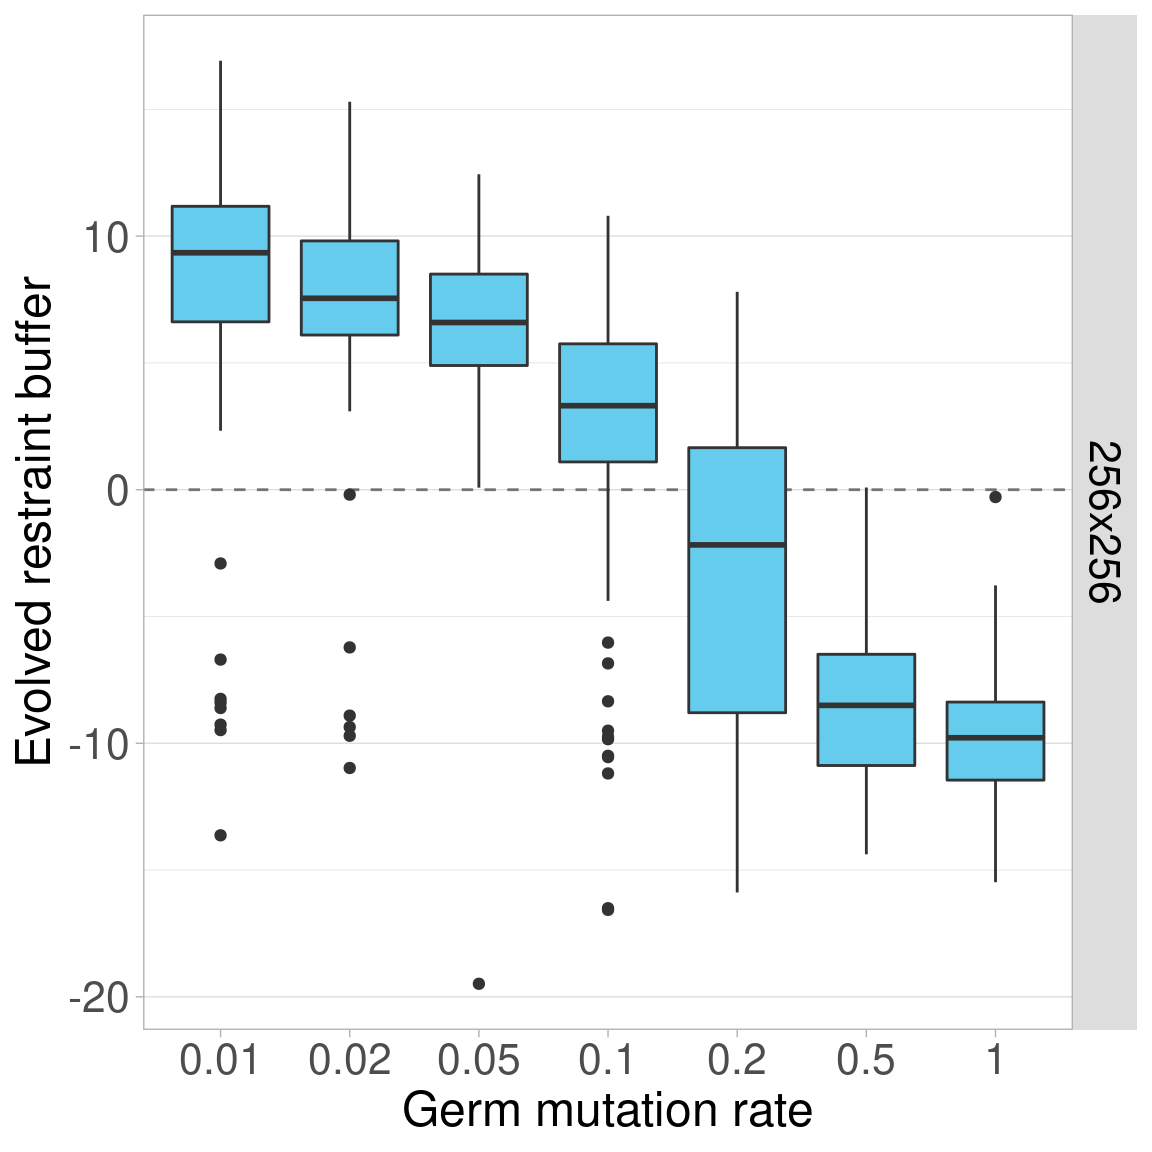
\includegraphics{primordium_supplemental_material_files/figure-latex/unnamed-chunk-38-1.pdf}

\hypertarget{aggregate-plots-2}{%
\section{Aggregate plots}\label{aggregate-plots-2}}

\hypertarget{facet-by-germ-mutation-rate}{%
\subsection{Facet by germ mutation rate}\label{facet-by-germ-mutation-rate}}

Here we plot all the data at once.
Each row shows a different germ mutation rate and each boxplot shows a given organism size.

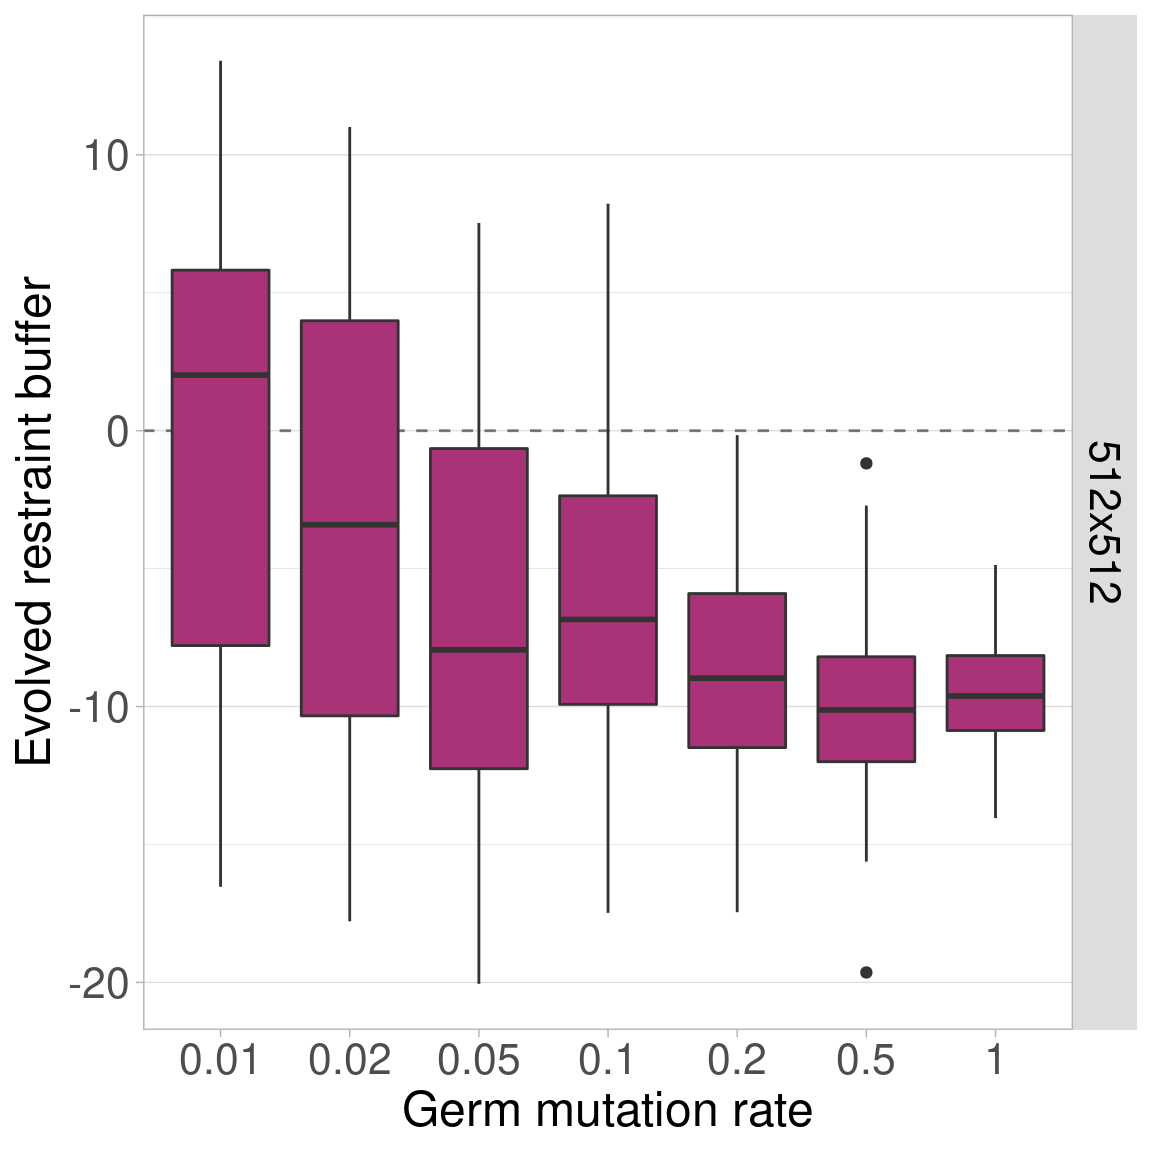
\includegraphics{primordium_supplemental_material_files/figure-latex/unnamed-chunk-39-1.pdf}

Here is the same data, plotted identically other than now each row can have a different y-axis.

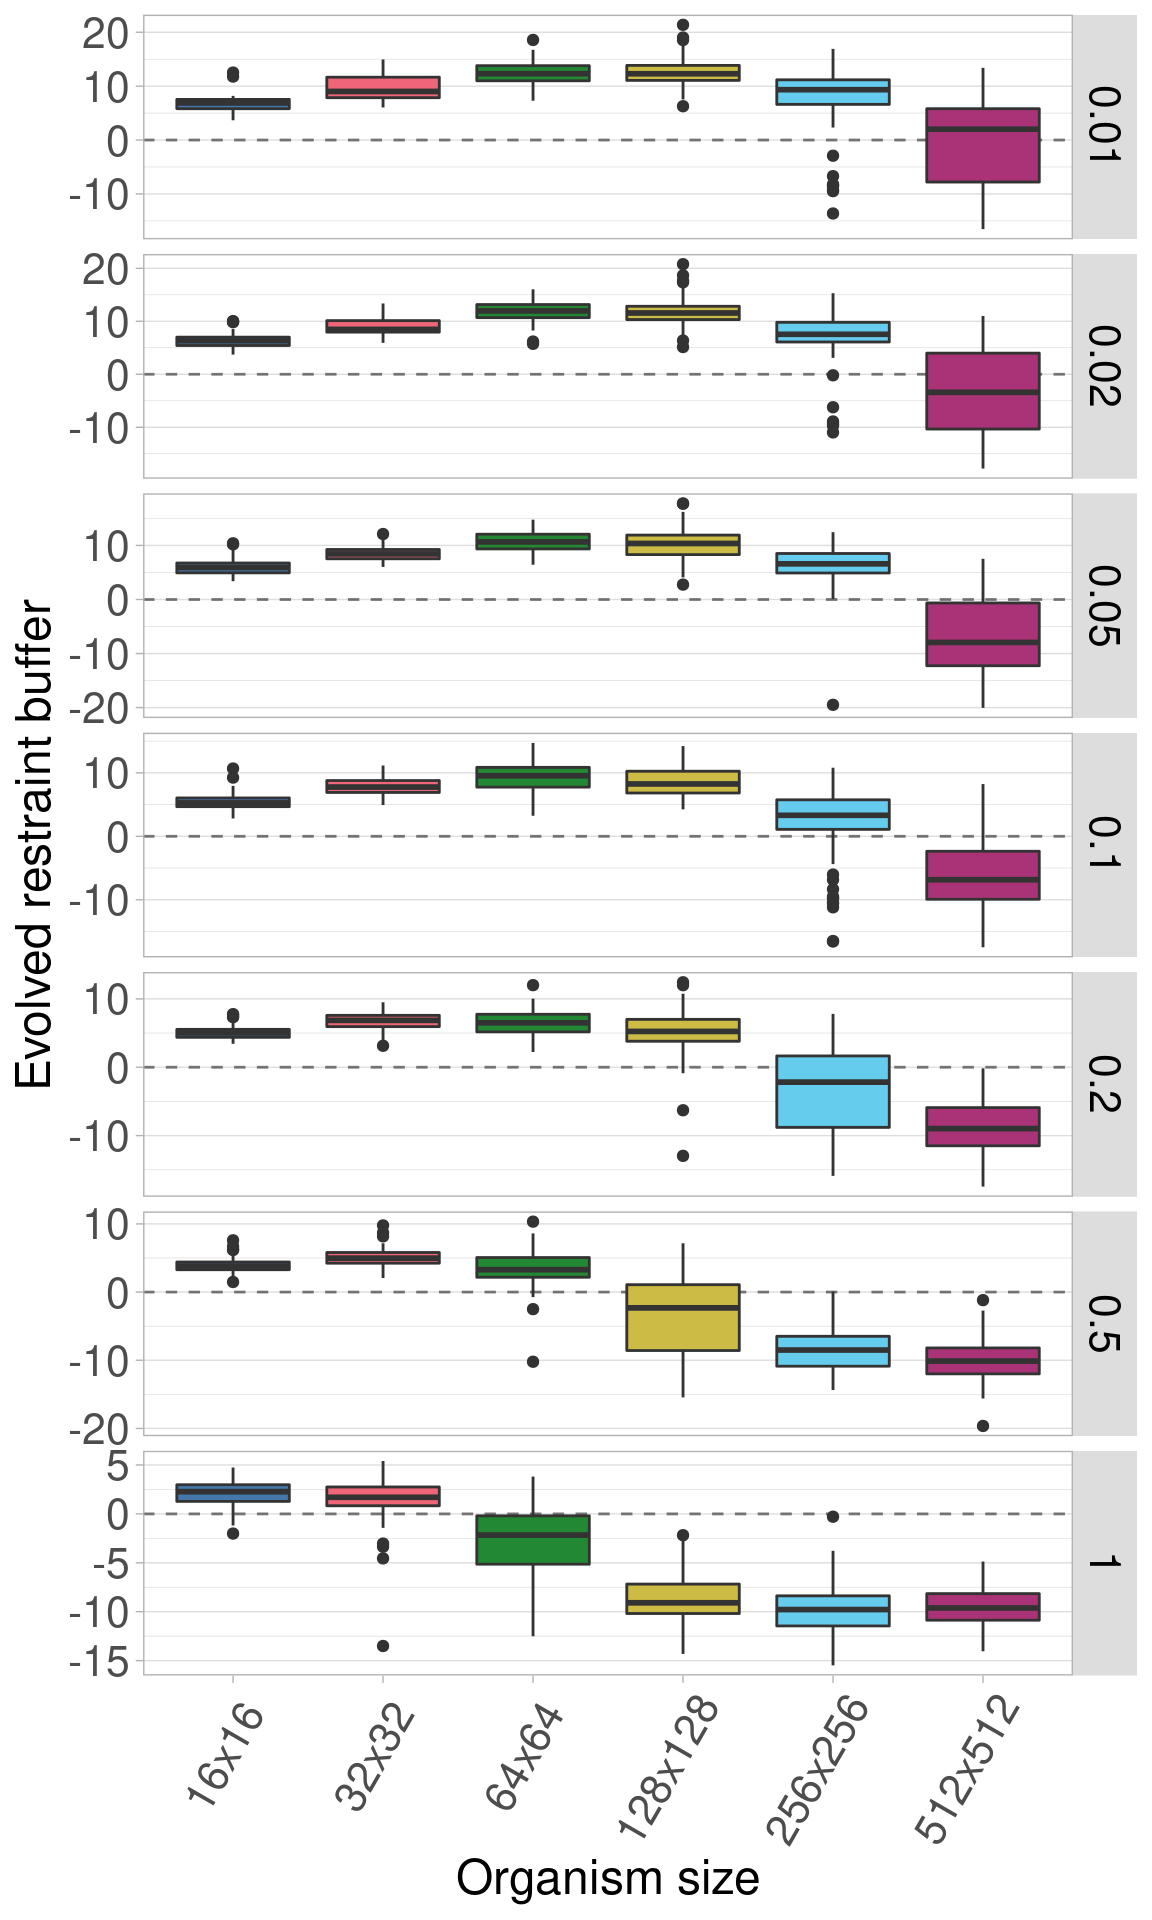
\includegraphics{primordium_supplemental_material_files/figure-latex/unnamed-chunk-40-1.pdf}

\hypertarget{facet-by-organism-size-1}{%
\subsection{Facet by organism size}\label{facet-by-organism-size-1}}

Next, we plot the same data, but this time each row corresponds to a certain organism size while germ mutation rate varies along the x-axis.

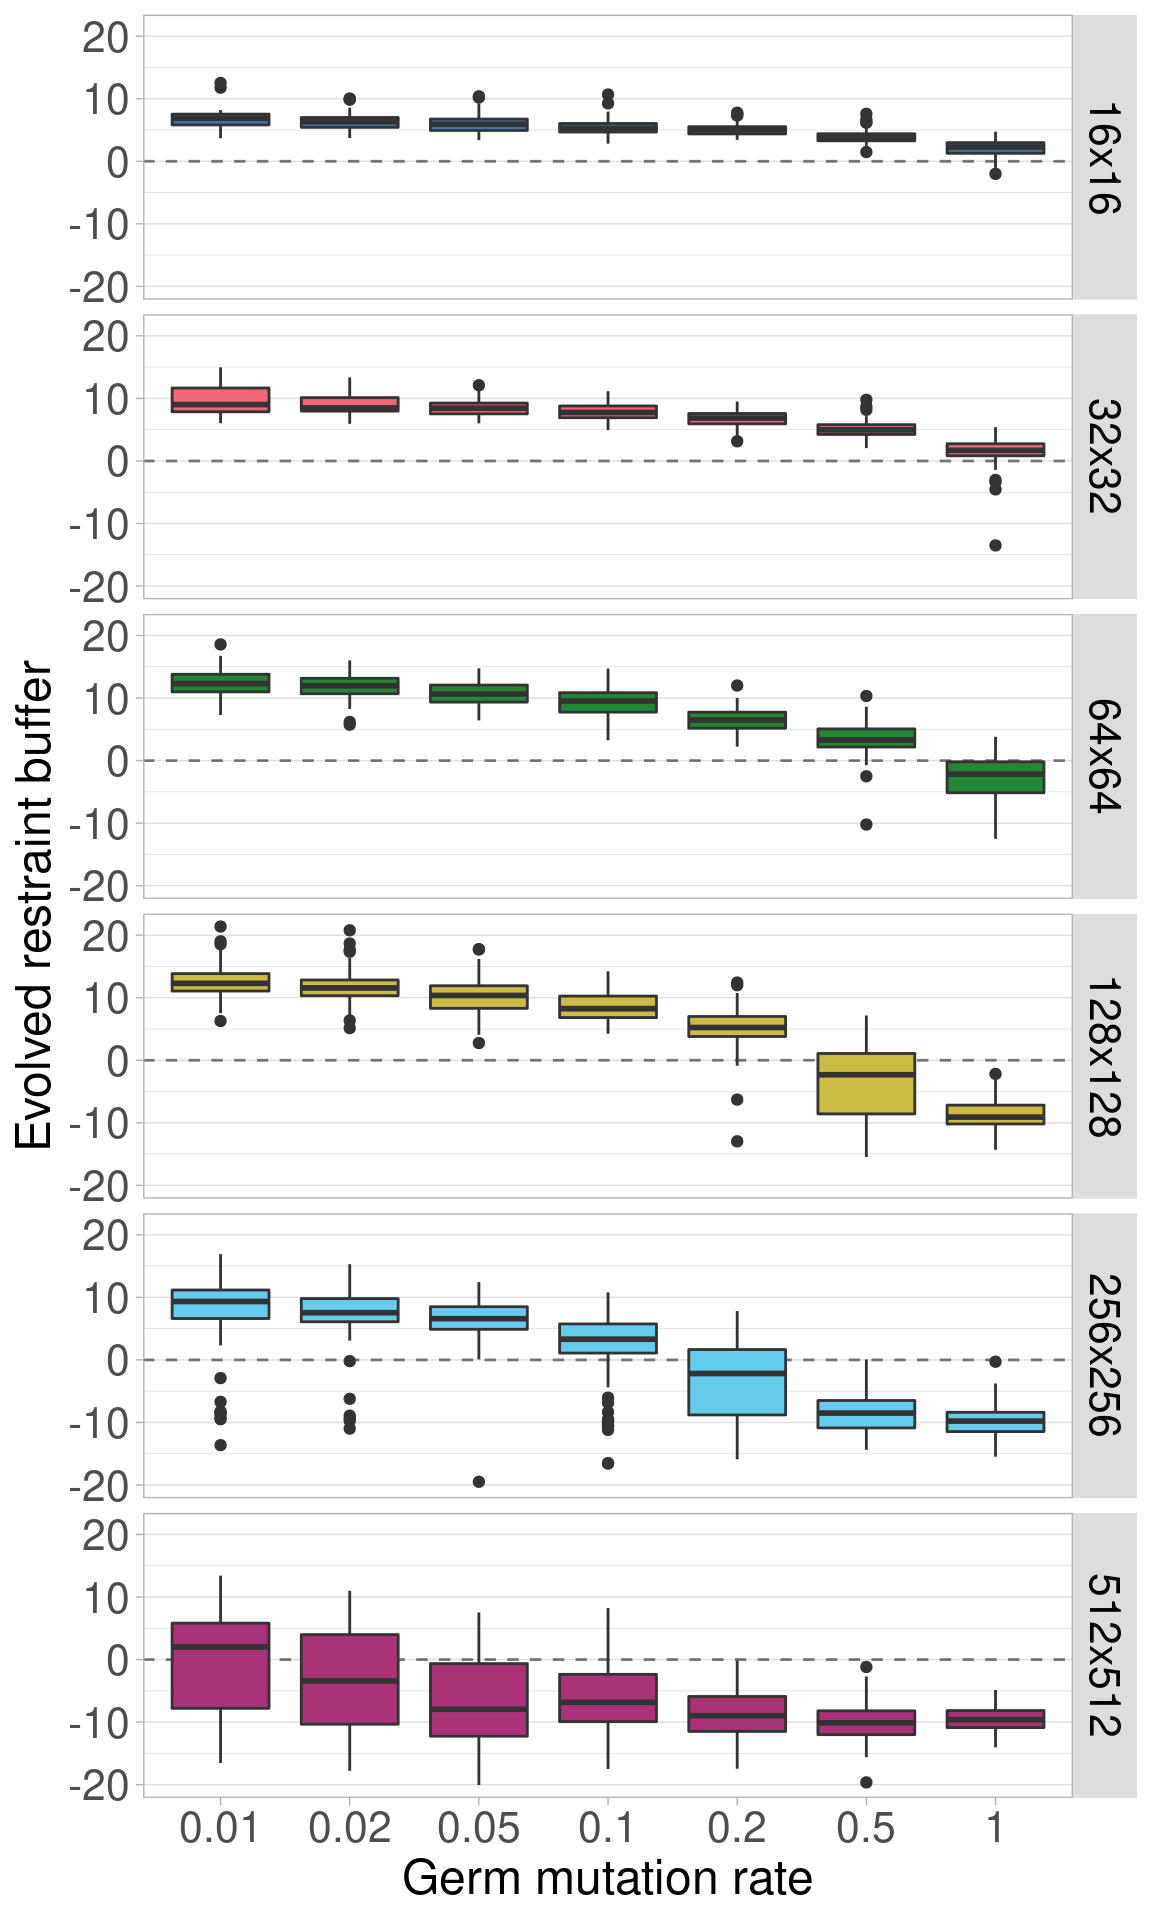
\includegraphics{primordium_supplemental_material_files/figure-latex/unnamed-chunk-41-1.pdf}

Again, we plot the same data again, but now the y-axis can change between rows.

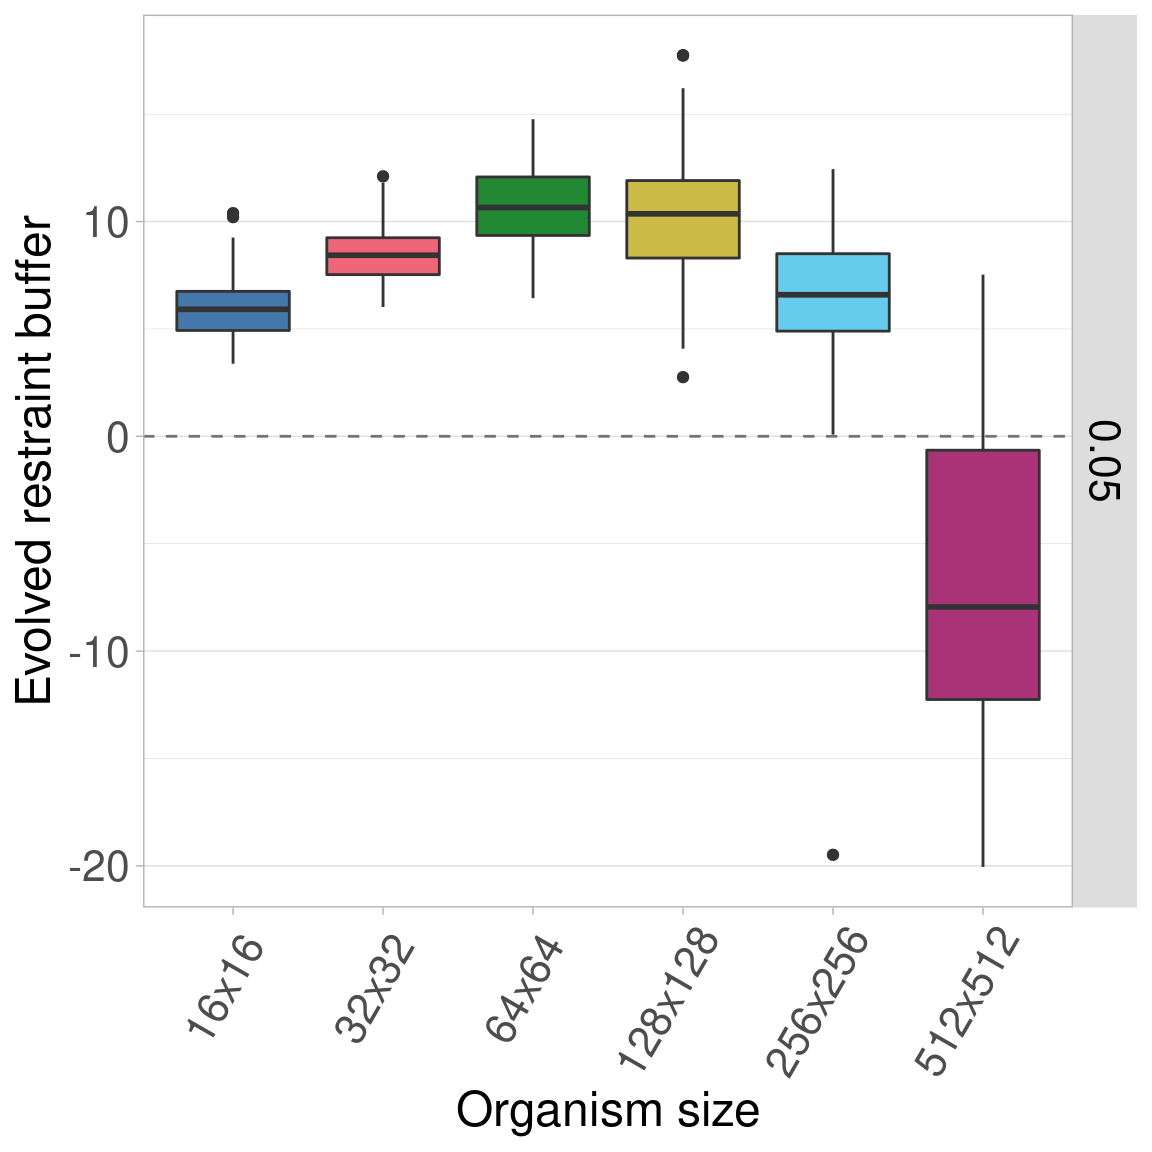
\includegraphics{primordium_supplemental_material_files/figure-latex/unnamed-chunk-42-1.pdf}

\hypertarget{single-organism-size-plots-1}{%
\section{Single organism size plots}\label{single-organism-size-plots-1}}

Here we plot each organism size independently, with the germ mutation rate on the x-axis.

\hypertarget{organism-size-16x16-1}{%
\subsection{Organism size 16x16}\label{organism-size-16x16-1}}

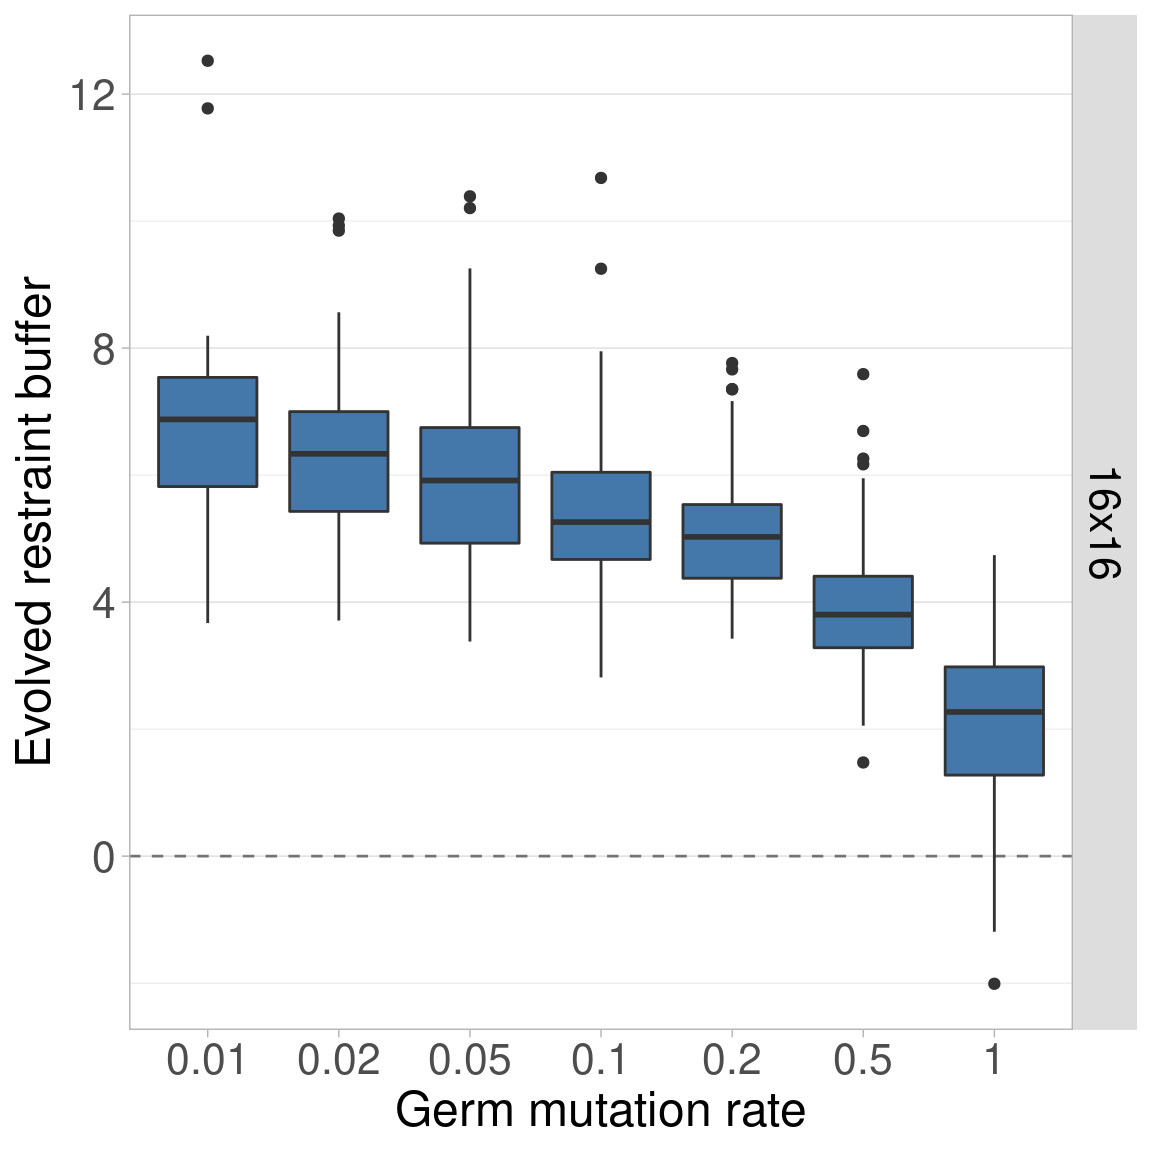
\includegraphics{primordium_supplemental_material_files/figure-latex/unnamed-chunk-43-1.pdf}

\hypertarget{organism-size-32x32-1}{%
\subsection{Organism size 32x32}\label{organism-size-32x32-1}}

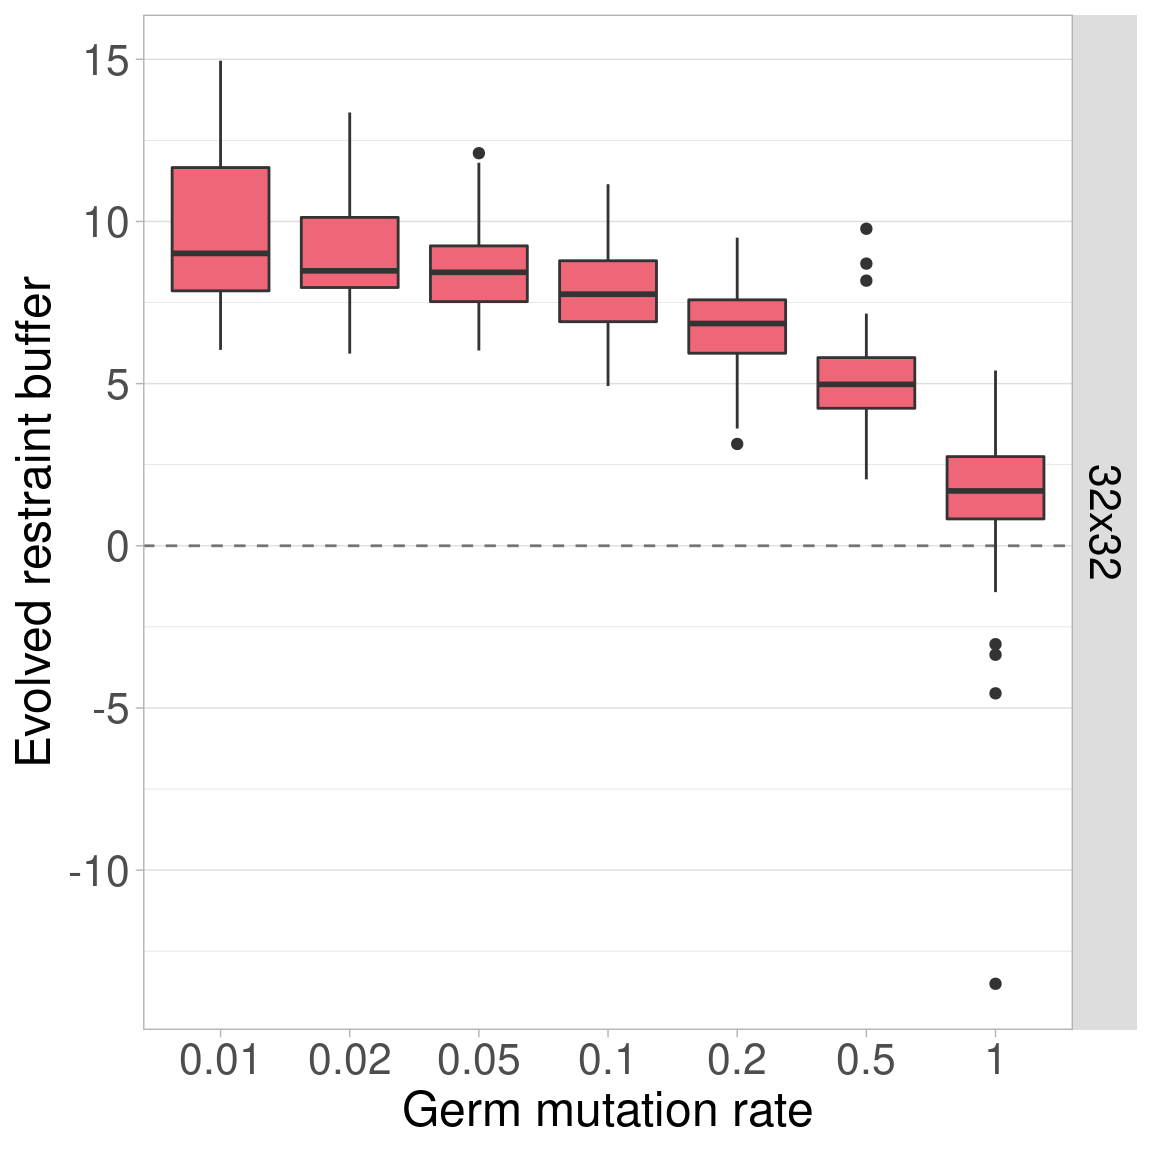
\includegraphics{primordium_supplemental_material_files/figure-latex/unnamed-chunk-44-1.pdf}

\hypertarget{organism-size-64x64-1}{%
\subsection{Organism size 64x64}\label{organism-size-64x64-1}}

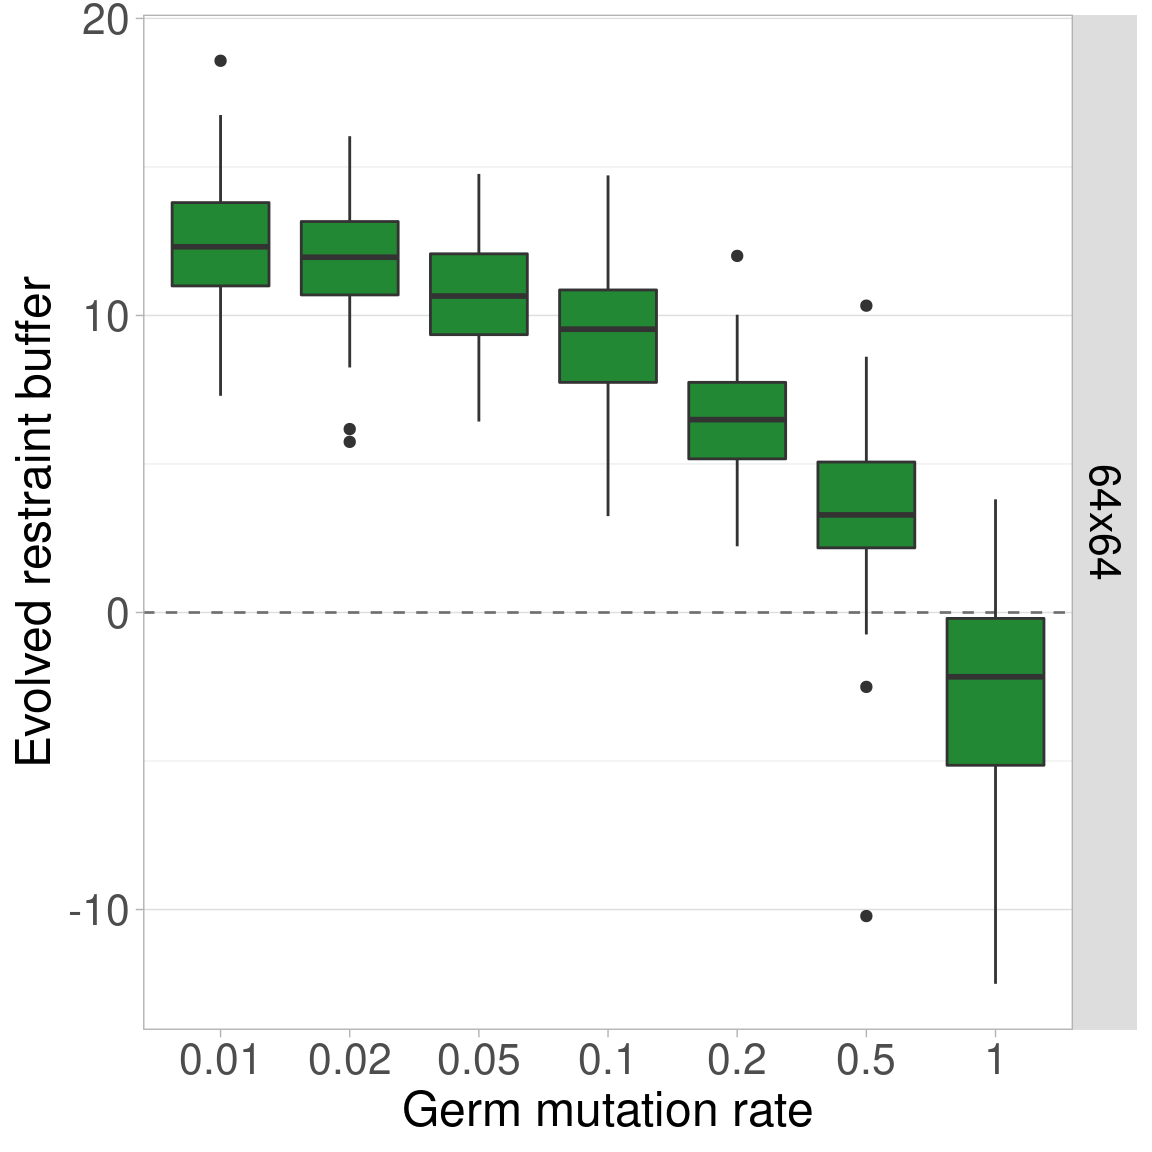
\includegraphics{primordium_supplemental_material_files/figure-latex/unnamed-chunk-45-1.pdf}

\hypertarget{organism-size-128x128-1}{%
\subsection{Organism size 128x128}\label{organism-size-128x128-1}}

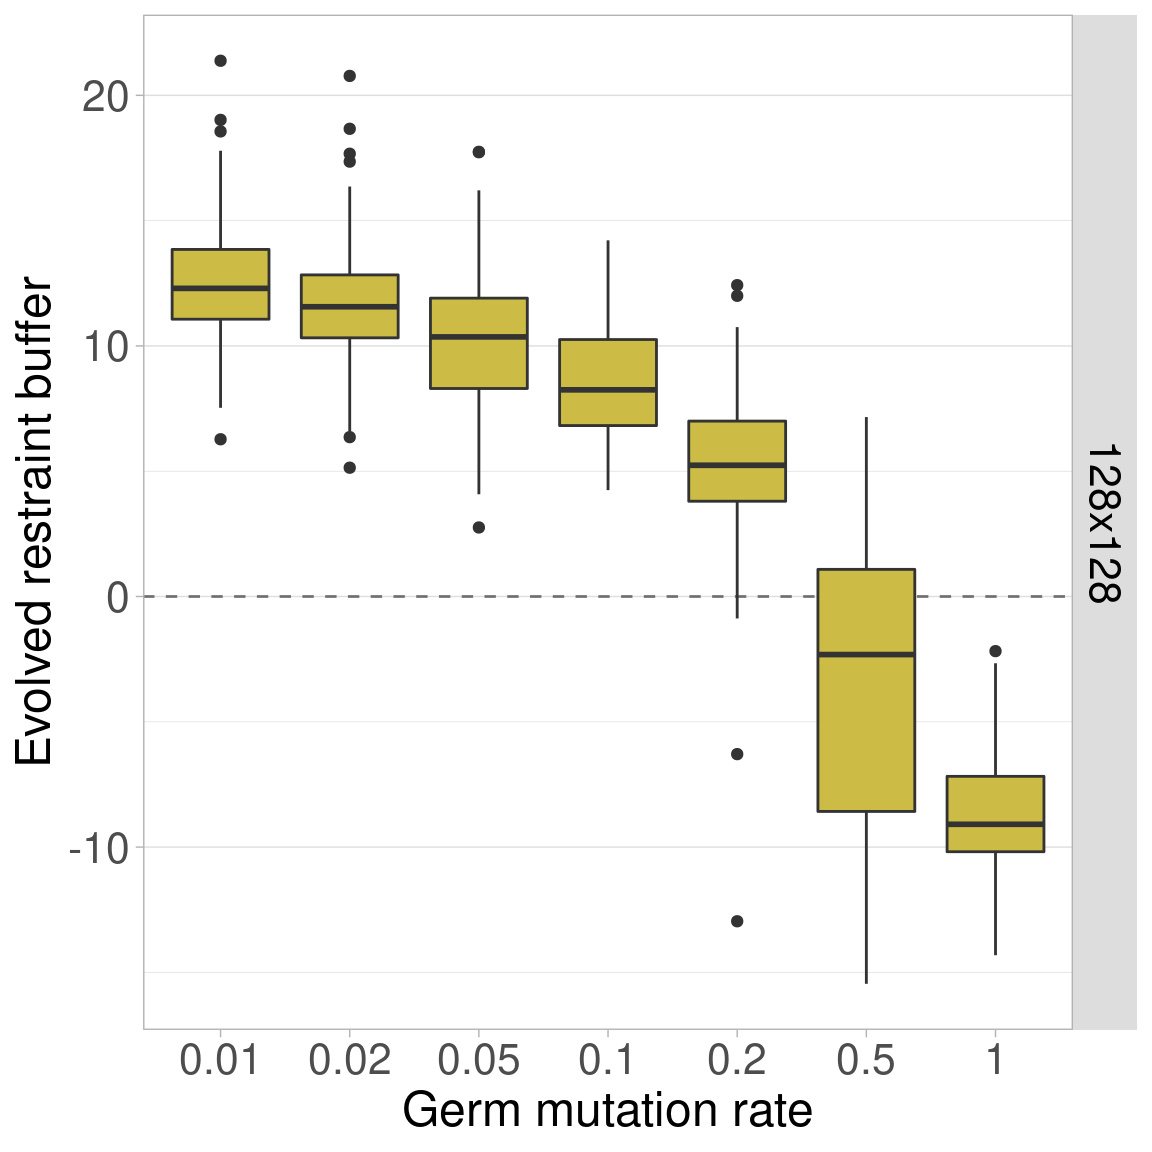
\includegraphics{primordium_supplemental_material_files/figure-latex/unnamed-chunk-46-1.pdf}

\hypertarget{organism-size-256x256-1}{%
\subsection{Organism size 256x256}\label{organism-size-256x256-1}}

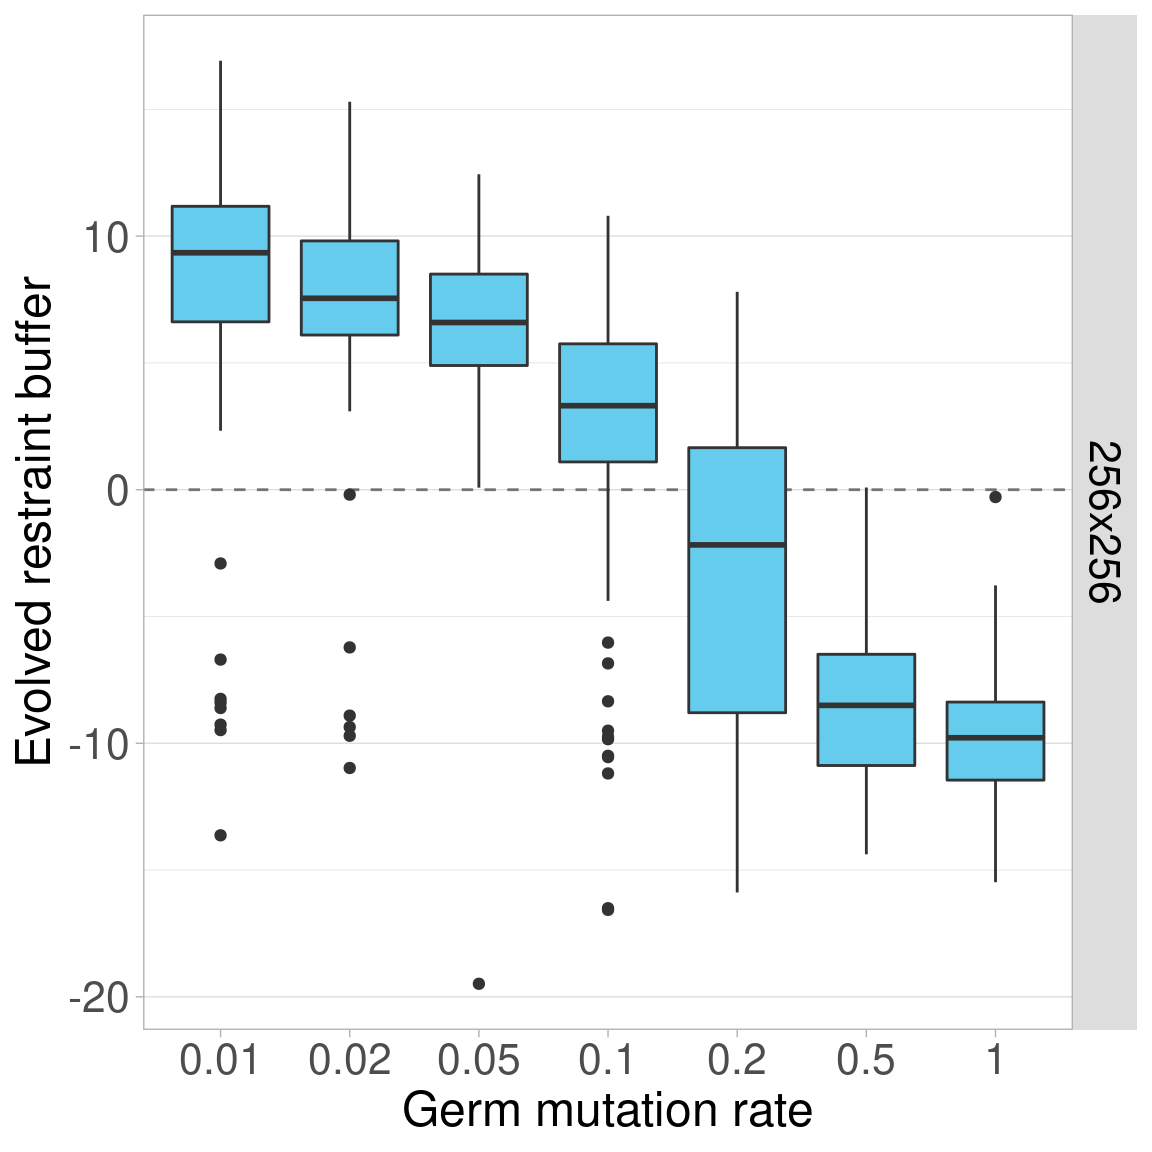
\includegraphics{primordium_supplemental_material_files/figure-latex/unnamed-chunk-47-1.pdf}

\hypertarget{organism-size-512x512-1}{%
\subsection{Organism size 512x512}\label{organism-size-512x512-1}}

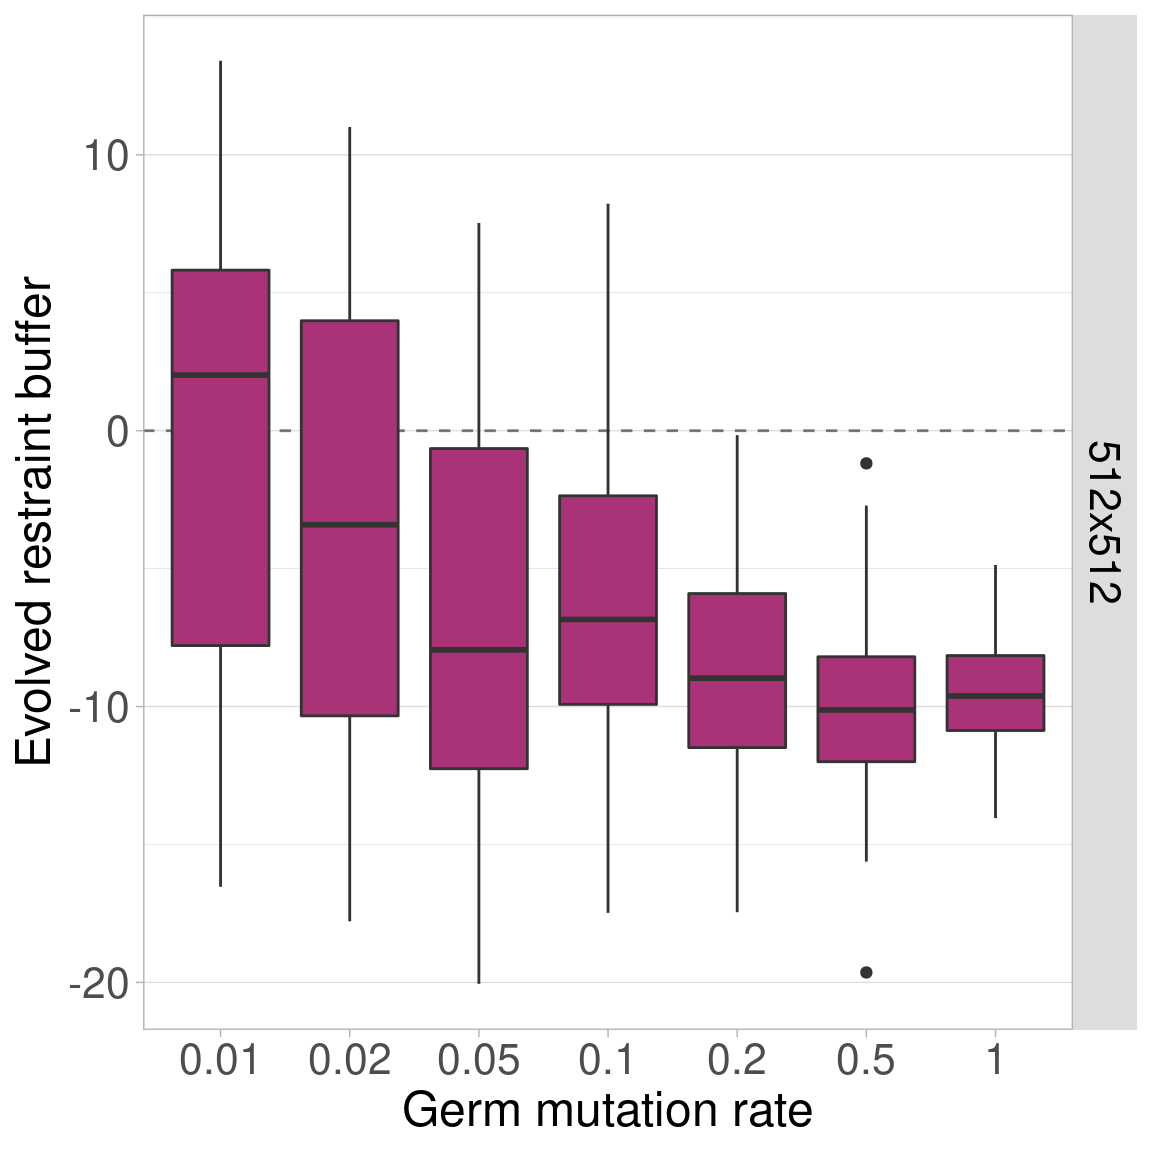
\includegraphics{primordium_supplemental_material_files/figure-latex/unnamed-chunk-48-1.pdf}

\hypertarget{single-organism-size-plots-2}{%
\section{Single organism size plots}\label{single-organism-size-plots-2}}

Similarly, here we plot each germ mutation rate independently, with the organism size on the x-axis.

\hypertarget{germ-mut.-rate-0.01}{%
\subsection{Germ mut. rate 0.01}\label{germ-mut.-rate-0.01}}

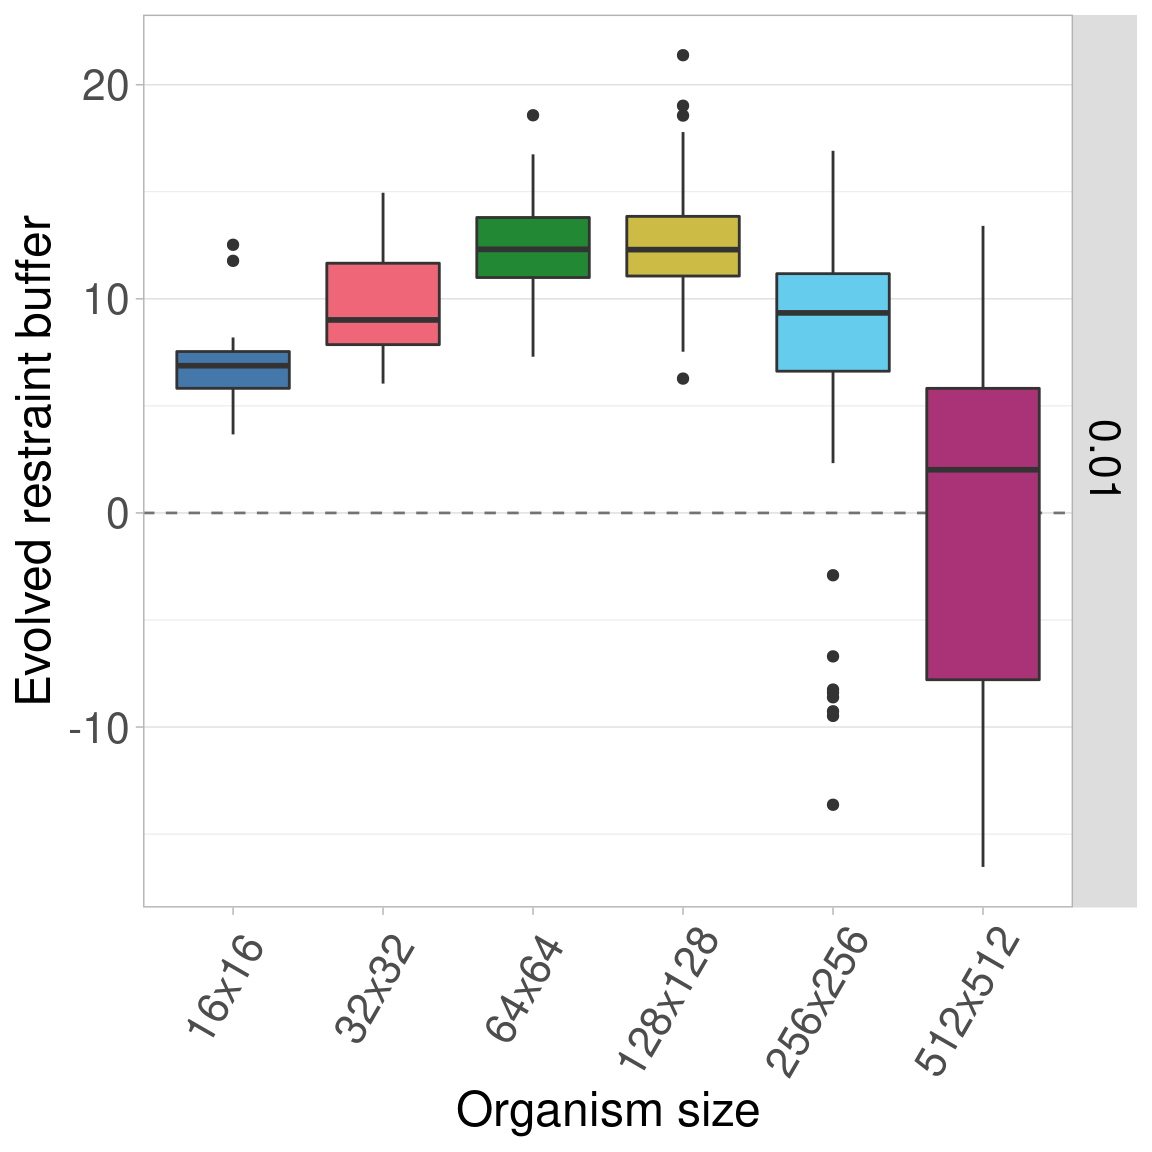
\includegraphics{primordium_supplemental_material_files/figure-latex/unnamed-chunk-49-1.pdf}

\hypertarget{germ-mut.-rate-0.02}{%
\subsection{Germ mut. rate 0.02}\label{germ-mut.-rate-0.02}}

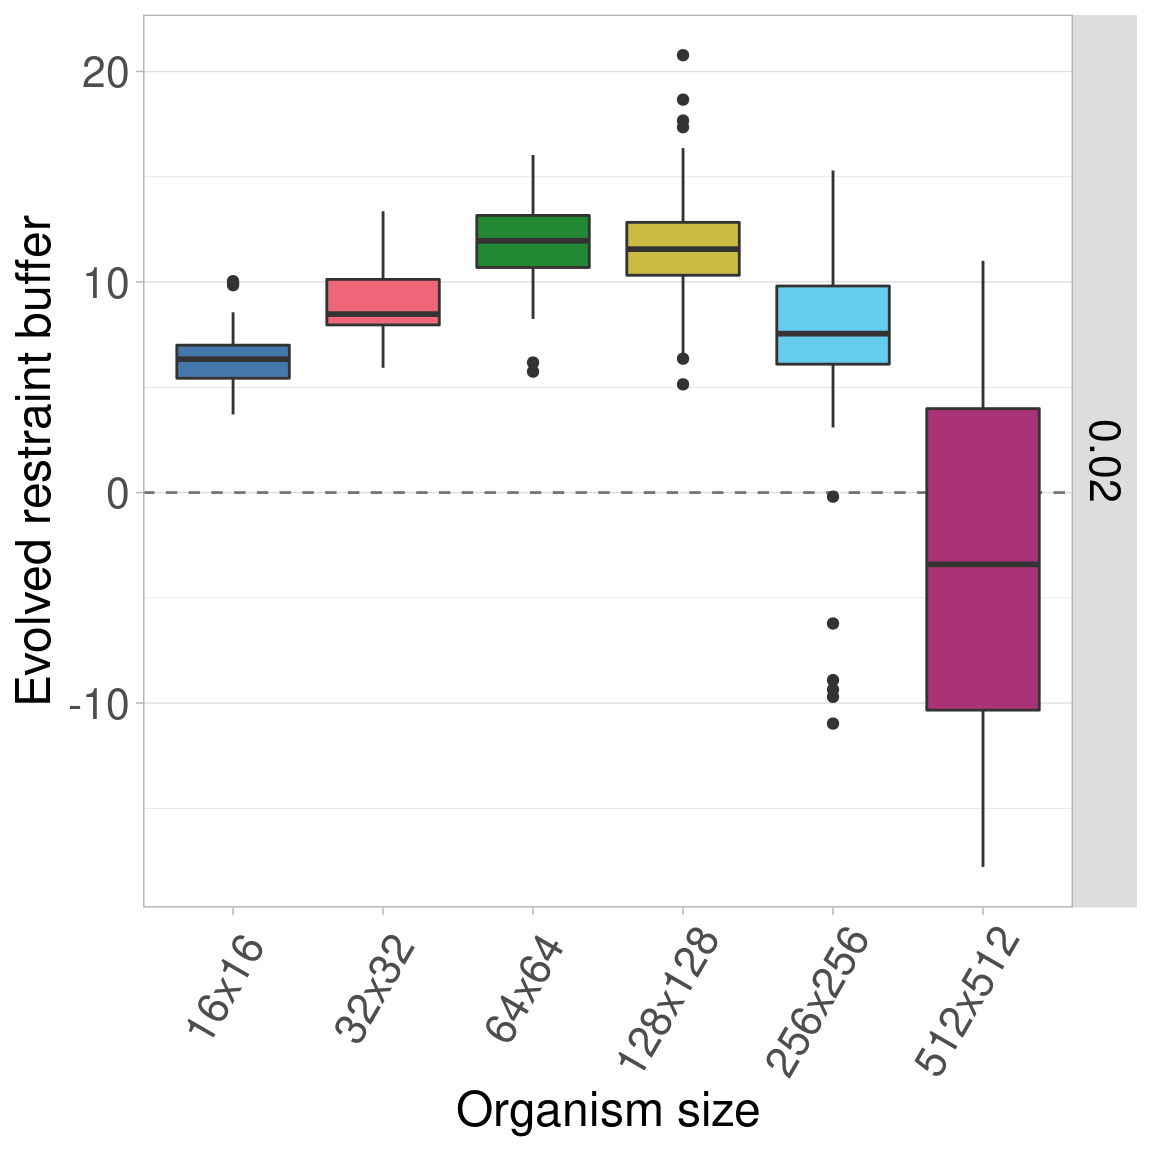
\includegraphics{primordium_supplemental_material_files/figure-latex/unnamed-chunk-50-1.pdf}

\hypertarget{germ-mut.-rate-0.05}{%
\subsection{Germ mut. rate 0.05}\label{germ-mut.-rate-0.05}}

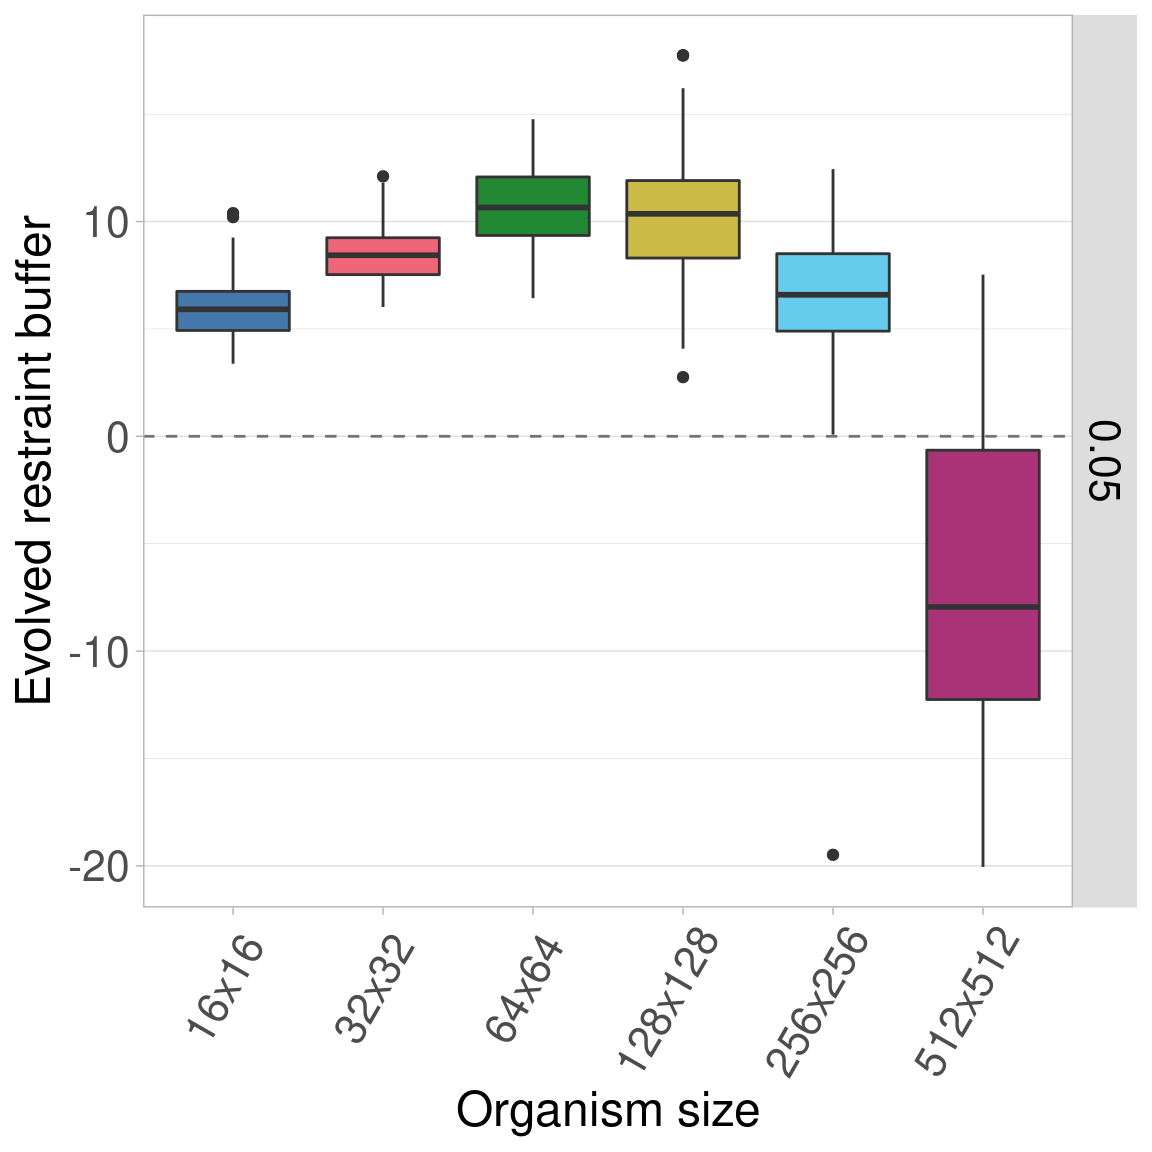
\includegraphics{primordium_supplemental_material_files/figure-latex/unnamed-chunk-51-1.pdf}

\hypertarget{germ-mut.-rate-0.1}{%
\subsection{Germ mut. rate 0.1}\label{germ-mut.-rate-0.1}}

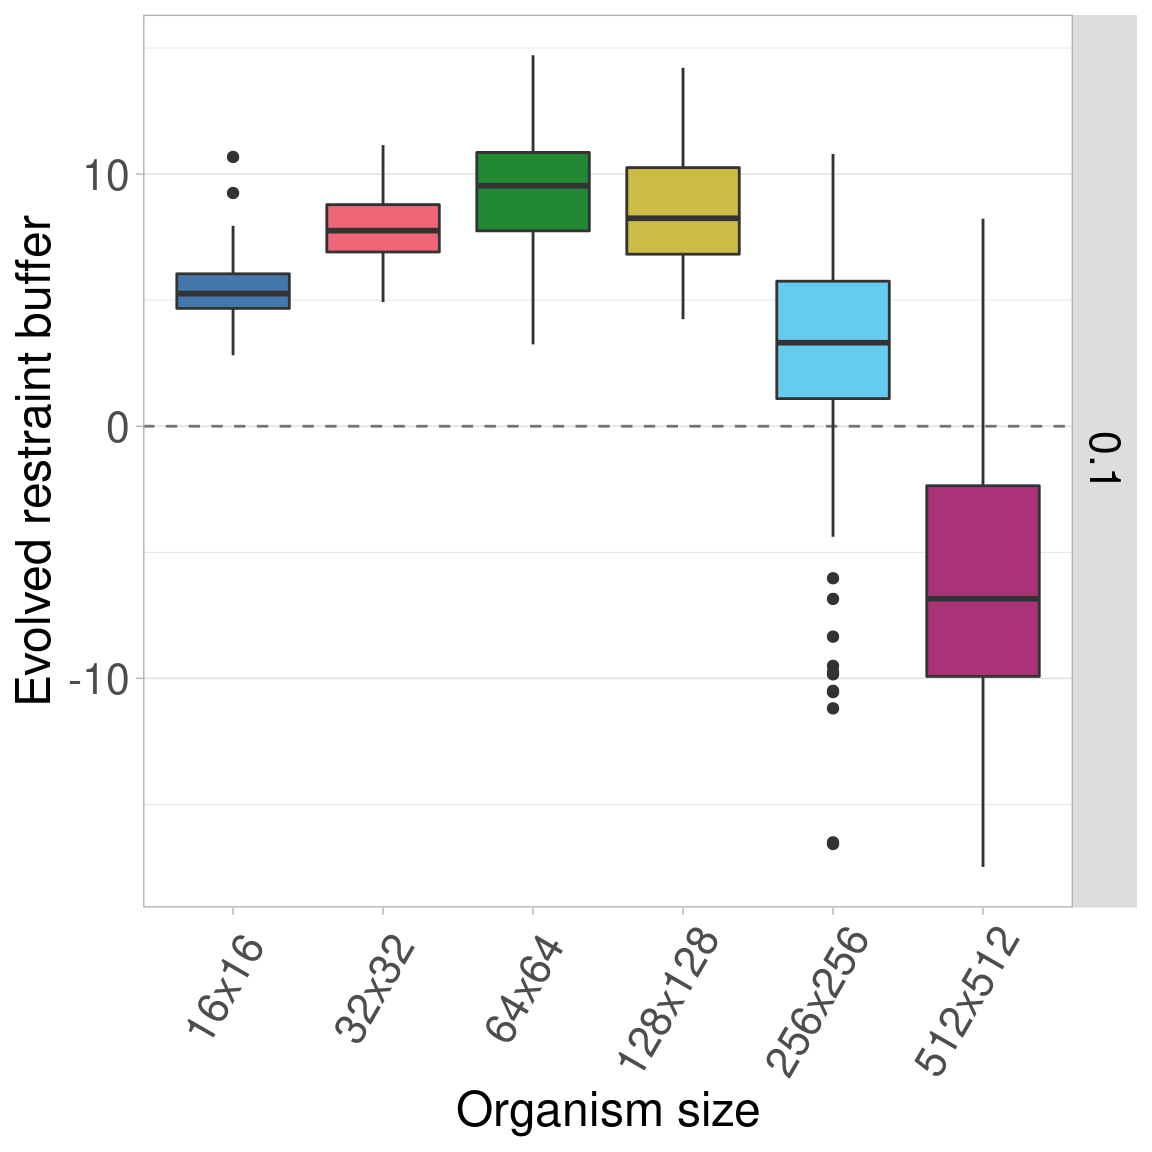
\includegraphics{primordium_supplemental_material_files/figure-latex/unnamed-chunk-52-1.pdf}

\hypertarget{germ-mut.-rate-0.2}{%
\subsection{Germ mut. rate 0.2}\label{germ-mut.-rate-0.2}}

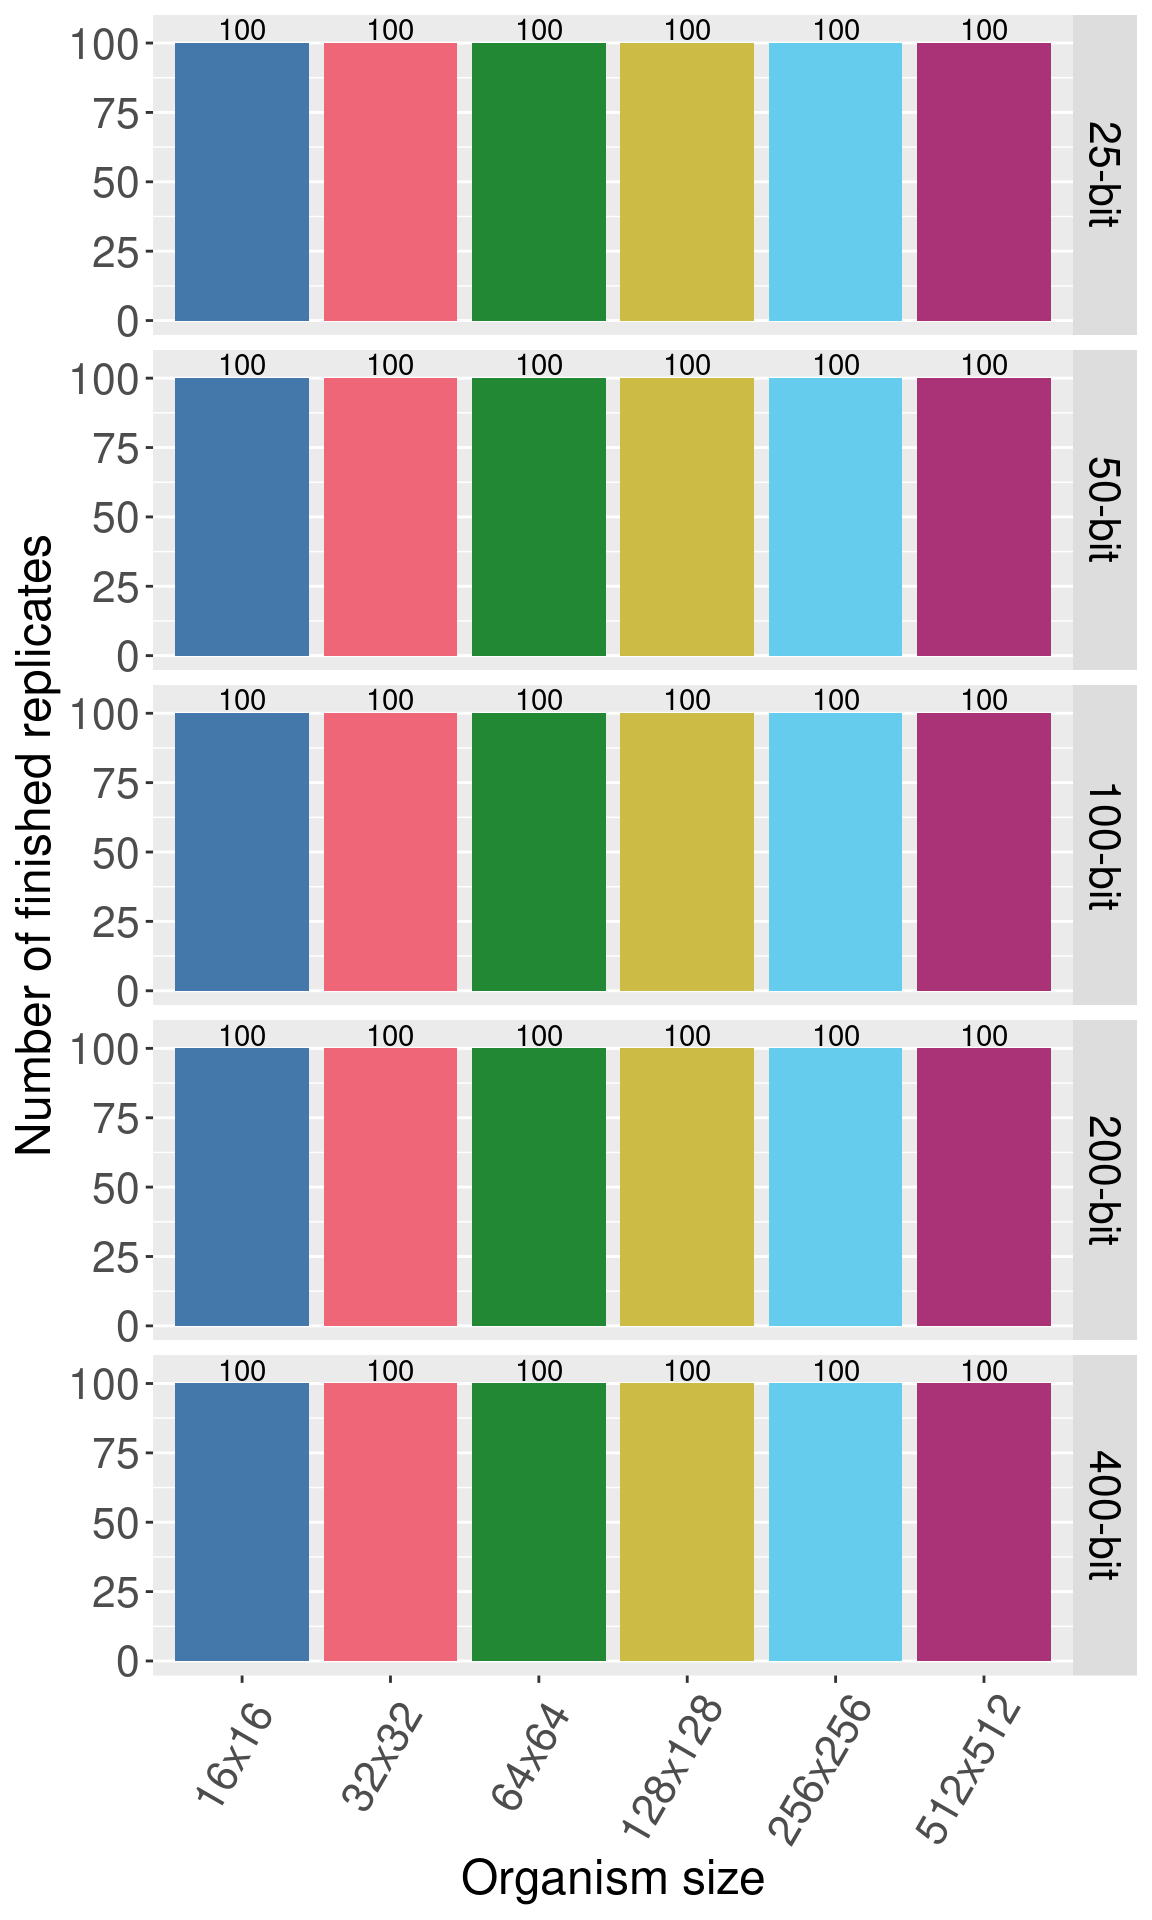
\includegraphics{primordium_supplemental_material_files/figure-latex/unnamed-chunk-53-1.pdf}

\hypertarget{germ-mut.-rate-0.5}{%
\subsection{Germ mut. rate 0.5}\label{germ-mut.-rate-0.5}}

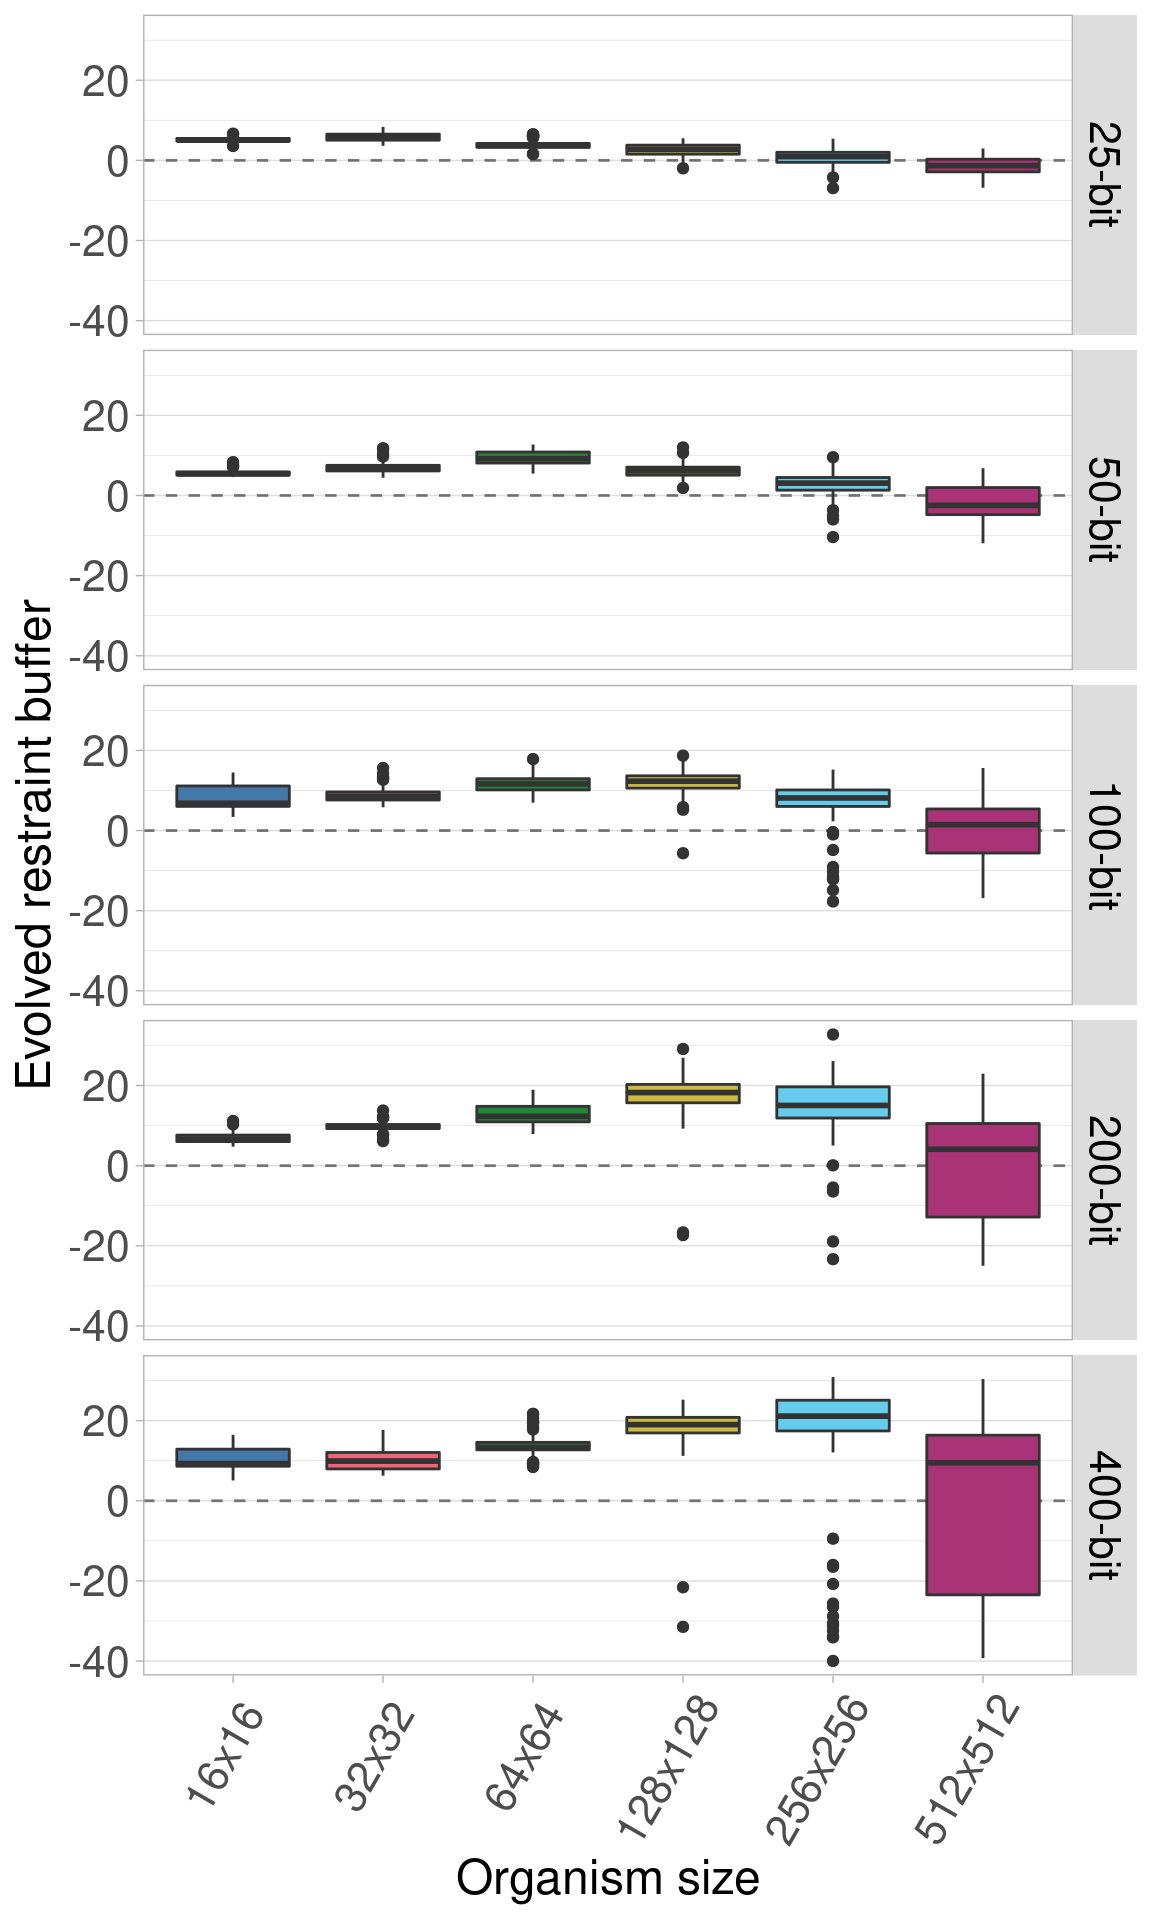
\includegraphics{primordium_supplemental_material_files/figure-latex/unnamed-chunk-54-1.pdf}

\hypertarget{germ-mut.-rate-1.0}{%
\subsection{Germ mut. rate 1.0}\label{germ-mut.-rate-1.0}}

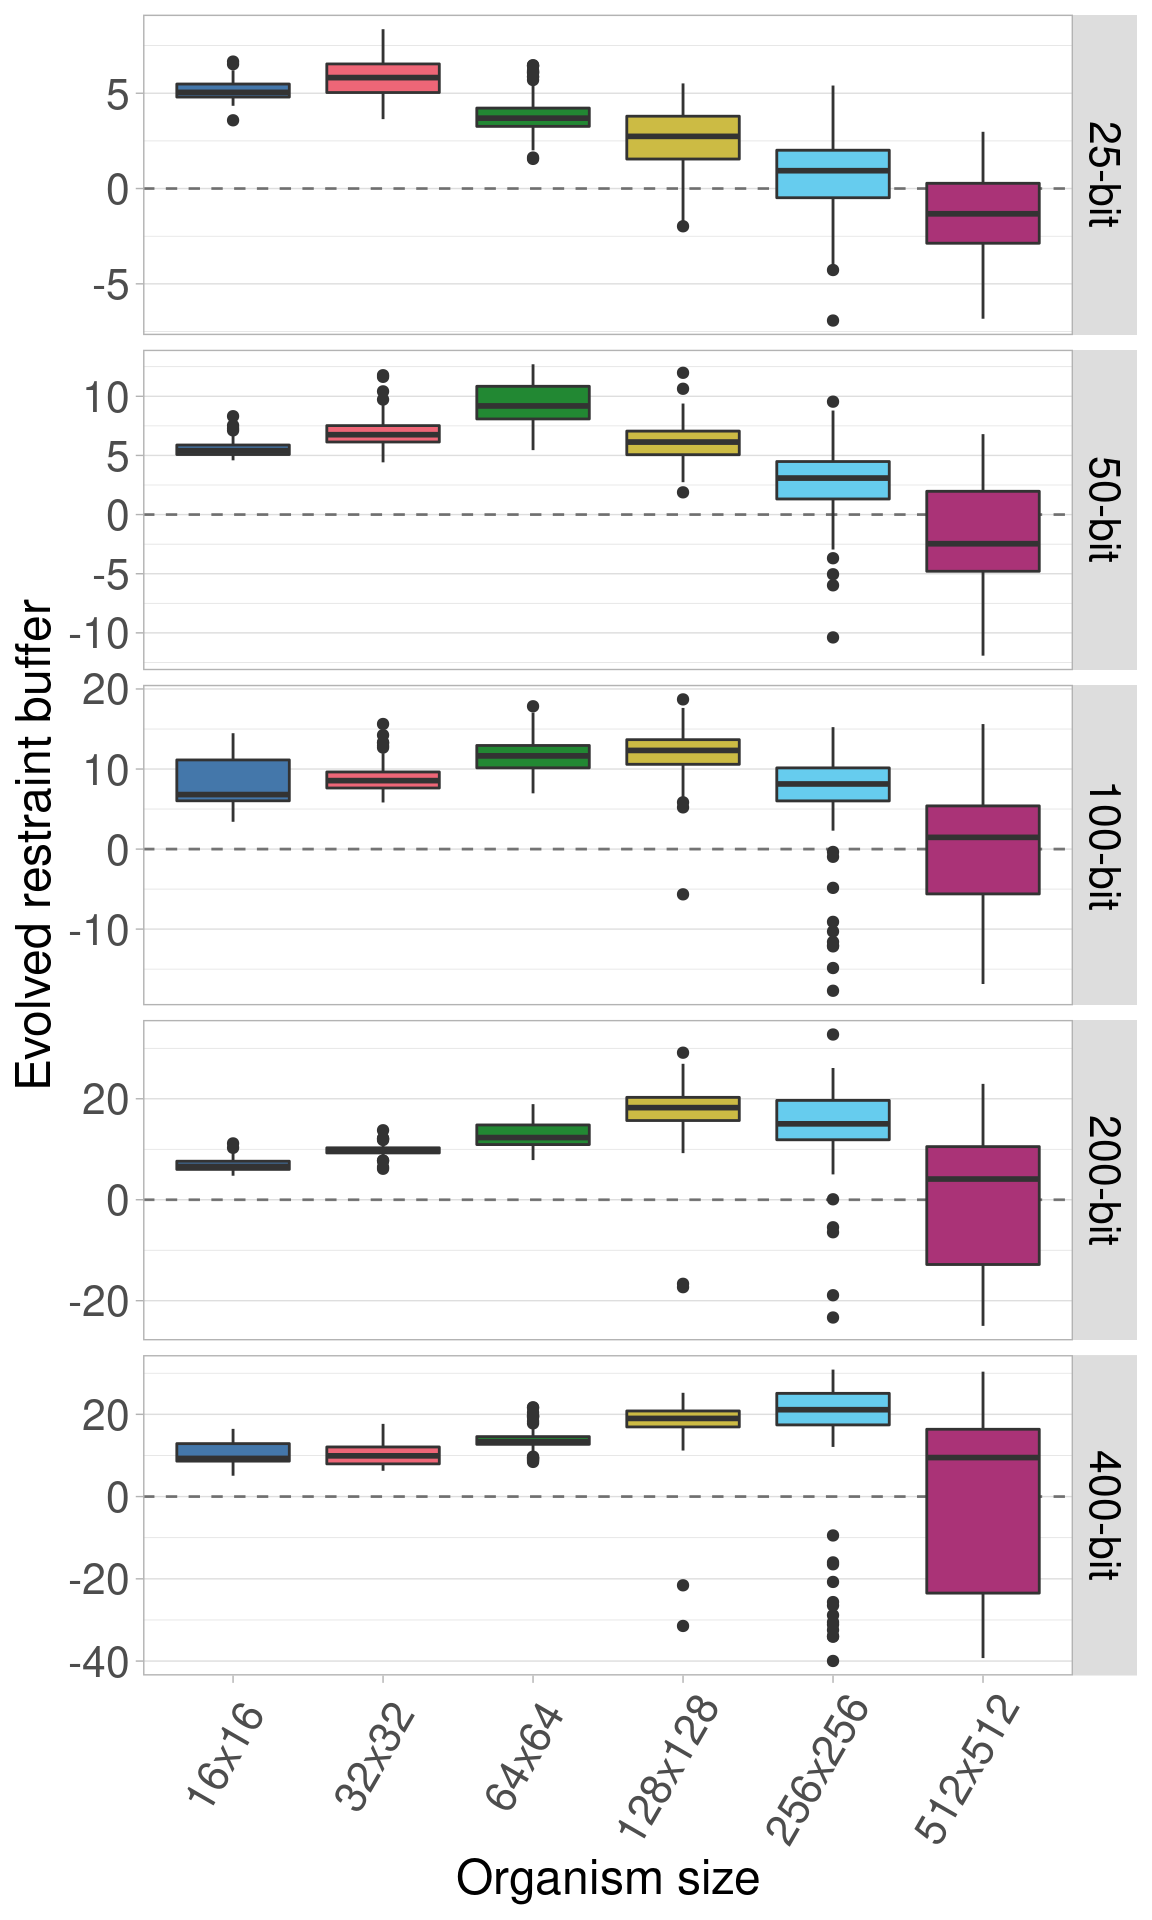
\includegraphics{primordium_supplemental_material_files/figure-latex/unnamed-chunk-55-1.pdf}

\hypertarget{statistics-2}{%
\section{Statistics}\label{statistics-2}}

Since organism size is our main point of comparison, we calculate stats for each germ mutation rate.

First, we perform a Kruskal-Wallis test across all organism sizes to indicate if variance exists at that mutation rate.
If variance exists, we then perform a pairwise Wilcoxon Rank-Sum test to show which pairs of organism sizes significantly differ.
Finally, we perform Bonferroni-Holm corrections for multiple comparisons.

\begin{Shaded}
\begin{Highlighting}[]
\NormalTok{  mut\_vec =}\StringTok{ }\KeywordTok{c}\NormalTok{(}\FloatTok{0.01}\NormalTok{, }\FloatTok{0.02}\NormalTok{, }\FloatTok{0.05}\NormalTok{, }\FloatTok{0.1}\NormalTok{, }\FloatTok{0.2}\NormalTok{, }\FloatTok{0.5}\NormalTok{, }\DecValTok{1}\NormalTok{)}
\NormalTok{  df\_kruskal =}\StringTok{ }\KeywordTok{data.frame}\NormalTok{(}\DataTypeTok{data =} \KeywordTok{matrix}\NormalTok{(}\DataTypeTok{nrow =} \DecValTok{0}\NormalTok{, }\DataTypeTok{ncol =} \DecValTok{4}\NormalTok{))}
  \KeywordTok{colnames}\NormalTok{(df\_kruskal) =}\StringTok{ }\KeywordTok{c}\NormalTok{(}\StringTok{\textquotesingle{}germ\_mut\_rate\textquotesingle{}}\NormalTok{, }\StringTok{\textquotesingle{}p\_value\textquotesingle{}}\NormalTok{, }\StringTok{\textquotesingle{}chi\_squared\textquotesingle{}}\NormalTok{, }\StringTok{\textquotesingle{}df\textquotesingle{}}\NormalTok{)}
  \ControlFlowTok{for}\NormalTok{(mut\_rate }\ControlFlowTok{in}\NormalTok{ mut\_vec)\{}
\NormalTok{    df\_test =}\StringTok{ }\NormalTok{df2[df2}\OperatorTok{$}\NormalTok{MUT }\OperatorTok{==}\StringTok{ }\NormalTok{mut\_rate,]}
\NormalTok{    res =}\StringTok{ }\KeywordTok{kruskal.test}\NormalTok{(df\_test}\OperatorTok{$}\NormalTok{restraint\_value }\OperatorTok{\textasciitilde{}}\StringTok{ }\NormalTok{df\_test}\OperatorTok{$}\NormalTok{MCSIZE, df\_test)}
\NormalTok{    df\_kruskal[}\KeywordTok{nrow}\NormalTok{(df\_kruskal) }\OperatorTok{+}\StringTok{ }\DecValTok{1}\NormalTok{,] =}\StringTok{ }\KeywordTok{c}\NormalTok{(mut\_rate, res}\OperatorTok{$}\NormalTok{p.value, }\KeywordTok{as.numeric}\NormalTok{(res}\OperatorTok{$}\NormalTok{statistic)[}\DecValTok{1}\NormalTok{], }\KeywordTok{as.numeric}\NormalTok{(res}\OperatorTok{$}\NormalTok{parameter)[}\DecValTok{1}\NormalTok{])}
\NormalTok{  \}}
\NormalTok{  df\_kruskal}\OperatorTok{$}\NormalTok{less\_}\FloatTok{0.01}\NormalTok{ =}\StringTok{ }\NormalTok{df\_kruskal}\OperatorTok{$}\NormalTok{p\_value }\OperatorTok{\textless{}}\StringTok{ }\FloatTok{0.01}
  \KeywordTok{print}\NormalTok{(df\_kruskal)}
\end{Highlighting}
\end{Shaded}

\begin{verbatim}
##   germ_mut_rate      p_value chi_squared df less_0.01
## 1          0.01 9.191452e-79    374.5160  5      TRUE
## 2          0.02 6.227269e-82    389.2251  5      TRUE
## 3          0.05 1.934895e-82    391.5809  5      TRUE
## 4          0.10 1.983976e-83    396.1708  5      TRUE
## 5          0.20 3.180895e-85    404.4991  5      TRUE
## 6          0.50 4.313881e-91    431.7152  5      TRUE
## 7          1.00 2.144229e-92    437.7600  5      TRUE
\end{verbatim}

We see that significant variation exists within each mutation rate, so we perform pairwise Wilcoxon tests on each to see which pairs of sizes are significantly different.

\begin{Shaded}
\begin{Highlighting}[]
\NormalTok{size\_vec =}\StringTok{ }\KeywordTok{c}\NormalTok{(}\DecValTok{16}\NormalTok{, }\DecValTok{32}\NormalTok{, }\DecValTok{64}\NormalTok{, }\DecValTok{128}\NormalTok{, }\DecValTok{256}\NormalTok{, }\DecValTok{512}\NormalTok{)}
\NormalTok{mut\_vec =}\StringTok{ }\KeywordTok{c}\NormalTok{(}\FloatTok{0.01}\NormalTok{, }\FloatTok{0.02}\NormalTok{, }\FloatTok{0.05}\NormalTok{, }\FloatTok{0.1}\NormalTok{, }\FloatTok{0.2}\NormalTok{, }\FloatTok{0.5}\NormalTok{, }\DecValTok{1}\NormalTok{)}
\ControlFlowTok{for}\NormalTok{(mut\_rate }\ControlFlowTok{in}\NormalTok{ mut\_vec)\{}
\NormalTok{  df\_test =}\StringTok{ }\NormalTok{df2[df2}\OperatorTok{$}\NormalTok{MUT }\OperatorTok{==}\StringTok{ }\NormalTok{mut\_rate,]}
\NormalTok{  df\_wilcox =}\StringTok{ }\KeywordTok{data.frame}\NormalTok{(}\DataTypeTok{data =} \KeywordTok{matrix}\NormalTok{(}\DataTypeTok{nrow =} \DecValTok{0}\NormalTok{, }\DataTypeTok{ncol =} \DecValTok{6}\NormalTok{))}
  \KeywordTok{colnames}\NormalTok{(df\_wilcox) =}\StringTok{ }\KeywordTok{c}\NormalTok{(}\StringTok{\textquotesingle{}germ\_mut\_rate\textquotesingle{}}\NormalTok{, }\StringTok{\textquotesingle{}size\_a\textquotesingle{}}\NormalTok{, }\StringTok{\textquotesingle{}size\_b\textquotesingle{}}\NormalTok{, }\StringTok{\textquotesingle{}p\_value\_corrected\textquotesingle{}}\NormalTok{, }\StringTok{\textquotesingle{}p\_value\_raw\textquotesingle{}}\NormalTok{, }\StringTok{\textquotesingle{}W\textquotesingle{}}\NormalTok{)}
  \ControlFlowTok{for}\NormalTok{(size\_idx\_a }\ControlFlowTok{in} \DecValTok{1}\OperatorTok{:}\NormalTok{(}\KeywordTok{length}\NormalTok{(size\_vec) }\OperatorTok{{-}}\StringTok{ }\DecValTok{1}\NormalTok{))\{}
\NormalTok{    size\_a =}\StringTok{ }\NormalTok{size\_vec[size\_idx\_a]}
    \ControlFlowTok{for}\NormalTok{(size\_idx\_b }\ControlFlowTok{in}\NormalTok{ (size\_idx\_a }\OperatorTok{+}\StringTok{ }\DecValTok{1}\NormalTok{)}\OperatorTok{:}\KeywordTok{length}\NormalTok{(size\_vec))\{}
\NormalTok{      size\_b =}\StringTok{ }\NormalTok{size\_vec[size\_idx\_b]}
\NormalTok{      res =}\StringTok{ }\KeywordTok{wilcox.test}\NormalTok{(df\_test[df\_test}\OperatorTok{$}\NormalTok{MCSIZE }\OperatorTok{==}\StringTok{ }\NormalTok{size\_a,]}\OperatorTok{$}\NormalTok{restraint\_value, df\_test[df\_test}\OperatorTok{$}\NormalTok{MCSIZE }\OperatorTok{==}\StringTok{ }\NormalTok{size\_b,]}\OperatorTok{$}\NormalTok{restraint\_value, }\DataTypeTok{alternative =} \StringTok{\textquotesingle{}two.sided\textquotesingle{}}\NormalTok{) }
\NormalTok{      df\_wilcox[}\KeywordTok{nrow}\NormalTok{(df\_wilcox) }\OperatorTok{+}\StringTok{ }\DecValTok{1}\NormalTok{,] =}\StringTok{ }\KeywordTok{c}\NormalTok{(mut\_rate, size\_a, size\_b, }\DecValTok{0}\NormalTok{, res}\OperatorTok{$}\NormalTok{p.value, }\KeywordTok{as.numeric}\NormalTok{(res}\OperatorTok{$}\NormalTok{statistic)[}\DecValTok{1}\NormalTok{])}
\NormalTok{    \}}
\NormalTok{  \}}
\NormalTok{  df\_wilcox}\OperatorTok{$}\NormalTok{p\_value\_corrected =}\StringTok{ }\KeywordTok{p.adjust}\NormalTok{(df\_wilcox}\OperatorTok{$}\NormalTok{p\_value\_raw, }\DataTypeTok{method =} \StringTok{\textquotesingle{}holm\textquotesingle{}}\NormalTok{)}
\NormalTok{  df\_wilcox}\OperatorTok{$}\NormalTok{less\_}\FloatTok{0.01}\NormalTok{ =}\StringTok{ }\NormalTok{df\_wilcox}\OperatorTok{$}\NormalTok{p\_value\_corrected }\OperatorTok{\textless{}}\StringTok{ }\FloatTok{0.01}
  \KeywordTok{print}\NormalTok{(}\KeywordTok{paste0}\NormalTok{(}\StringTok{\textquotesingle{}Germ mutation rate: \textquotesingle{}}\NormalTok{, mut\_rate))}
  \KeywordTok{print}\NormalTok{(df\_wilcox)}
\NormalTok{\}}
\end{Highlighting}
\end{Shaded}

\begin{verbatim}
## [1] "Germ mutation rate: 0.01"
##    germ_mut_rate size_a size_b p_value_corrected  p_value_raw      W less_0.01
## 1           0.01     16     32      1.161192e-21 1.161192e-22  990.0      TRUE
## 2           0.01     16     64      1.990837e-31 1.484433e-32  137.0      TRUE
## 3           0.01     16    128      2.032847e-30 1.694039e-31  221.0      TRUE
## 4           0.01     16    256      1.721090e-07 5.736966e-08 2778.5      TRUE
## 5           0.01     16    512      1.237738e-13 2.062896e-14 8130.0      TRUE
## 6           0.01     32     64      4.401194e-15 5.501492e-16 1684.5      TRUE
## 7           0.01     32    128      1.423615e-13 2.847230e-14 1887.0      TRUE
## 8           0.01     32    256      2.438849e-01 1.219425e-01 5633.5     FALSE
## 9           0.01     32    512      5.140604e-27 4.673276e-28 9495.0      TRUE
## 10          0.01     64    128      9.221418e-01 9.221418e-01 5040.5     FALSE
## 11          0.01     64    256      4.110744e-14 5.872491e-15 8195.5      TRUE
## 12          0.01     64    512      6.122051e-32 4.081368e-33 9907.0      TRUE
## 13          0.01    128    256      5.020912e-13 1.255228e-13 8033.5      TRUE
## 14          0.01    128    512      1.990837e-31 1.422026e-32 9864.5      TRUE
## 15          0.01    256    512      1.882508e-17 2.091675e-18 8582.5      TRUE
## [1] "Germ mutation rate: 0.02"
##    germ_mut_rate size_a size_b p_value_corrected  p_value_raw      W less_0.01
## 1           0.02     16     32      5.385908e-24 5.385908e-25  773.5      TRUE
## 2           0.02     16     64      3.620092e-31 2.585780e-32  156.0      TRUE
## 3           0.02     16    128      5.876058e-29 4.896715e-30  339.5      TRUE
## 4           0.02     16    256      7.355430e-06 2.451810e-06 3071.0      TRUE
## 5           0.02     16    512      2.935849e-18 3.669812e-19 8662.0      TRUE
## 6           0.02     32     64      5.800574e-18 8.286535e-19 1375.0      TRUE
## 7           0.02     32    128      4.715120e-12 1.178780e-12 2090.5      TRUE
## 8           0.02     32    256      4.080762e-04 2.040381e-04 6520.5      TRUE
## 9           0.02     32    512      6.645814e-27 6.041649e-28 9485.5      TRUE
## 10          0.02     64    128      2.889472e-01 2.889472e-01 5434.5     FALSE
## 11          0.02     64    256      2.039804e-17 3.399674e-18 8560.0      TRUE
## 12          0.02     64    512      4.109271e-32 2.739514e-33 9920.5      TRUE
## 13          0.02    128    256      2.514342e-14 5.028683e-15 8203.5      TRUE
## 14          0.02    128    512      4.123142e-31 3.171647e-32 9837.0      TRUE
## 15          0.02    256    512      4.866893e-20 5.407659e-21 8848.0      TRUE
## [1] "Germ mutation rate: 0.05"
##    germ_mut_rate size_a size_b p_value_corrected  p_value_raw      W less_0.01
## 1           0.05     16     32      1.591362e-24 1.768180e-25  730.0      TRUE
## 2           0.05     16     64      1.063762e-30 8.864684e-32  198.5      TRUE
## 3           0.05     16    128      3.321119e-21 4.151399e-22 1043.0      TRUE
## 4           0.05     16    256      2.538532e-02 1.269266e-02 3979.5     FALSE
## 5           0.05     16    512      1.050337e-26 9.548517e-28 9468.5      TRUE
## 6           0.05     32     64      3.387540e-14 5.645899e-15 1802.5      TRUE
## 7           0.05     32    128      1.306936e-05 4.356453e-06 3119.5      TRUE
## 8           0.05     32    256      1.528740e-07 3.821850e-08 7251.0      TRUE
## 9           0.05     32    512      3.162116e-32 2.258654e-33 9927.0      TRUE
## 10          0.05     64    128      1.546546e-01 1.546546e-01 5583.0     FALSE
## 11          0.05     64    256      4.390965e-19 6.272808e-20 8741.0      TRUE
## 12          0.05     64    512      6.208612e-33 4.139074e-34 9984.0      TRUE
## 13          0.05    128    256      2.838701e-12 5.677403e-13 7950.5      TRUE
## 14          0.05    128    512      9.845016e-32 7.573090e-33 9886.0      TRUE
## 15          0.05    256    512      3.142822e-26 3.142822e-27 9424.0      TRUE
## [1] "Germ mutation rate: 0.1"
##    germ_mut_rate size_a size_b p_value_corrected  p_value_raw      W less_0.01
## 1            0.1     16     32      2.006447e-24 2.229385e-25  739.0      TRUE
## 2            0.1     16     64      2.197505e-25 1.997732e-26  646.0      TRUE
## 3            0.1     16    128      3.982057e-19 6.636762e-20 1261.5      TRUE
## 4            0.1     16    256      2.853915e-06 9.513050e-07 7006.5      TRUE
## 5            0.1     16    512      1.146029e-26 9.550238e-28 9468.5      TRUE
## 6            0.1     32     64      6.866683e-07 1.716671e-07 2860.0      TRUE
## 7            0.1     32    128      5.714627e-02 5.714627e-02 4221.0     FALSE
## 8            0.1     32    256      7.451552e-21 9.314440e-22 8923.0      TRUE
## 9            0.1     32    512      1.091653e-31 7.797522e-33 9885.0      TRUE
## 10           0.1     64    128      2.618271e-02 1.309135e-02 6016.0     FALSE
## 11           0.1     64    256      6.893655e-25 6.893655e-26 9306.5      TRUE
## 12           0.1     64    512      4.295636e-32 2.863757e-33 9919.0      TRUE
## 13           0.1    128    256      9.294756e-21 1.327822e-21 8908.0      TRUE
## 14           0.1    128    512      2.475810e-31 1.904469e-32 9854.5      TRUE
## 15           0.1    256    512      7.440793e-16 1.488159e-16 8380.0      TRUE
## [1] "Germ mutation rate: 0.2"
##    germ_mut_rate size_a size_b p_value_corrected  p_value_raw       W less_0.01
## 1            0.2     16     32      6.711164e-17 9.587377e-18  1488.5      TRUE
## 2            0.2     16     64      2.652853e-08 5.305706e-09  2610.5      TRUE
## 3            0.2     16    128      5.723537e-01 4.033561e-01  4657.5     FALSE
## 4            0.2     16    256      9.414689e-28 1.046077e-28  9550.0      TRUE
## 5            0.2     16    512      3.841700e-33 2.561134e-34 10000.0      TRUE
## 6            0.2     32     64      5.723537e-01 2.861769e-01  5437.0     FALSE
## 7            0.2     32    128      2.713788e-06 6.784470e-07  7033.5      TRUE
## 8            0.2     32    256      2.557355e-30 2.324869e-31  9768.0      TRUE
## 9            0.2     32    512      3.841700e-33 2.561422e-34 10000.0      TRUE
## 10           0.2     64    128      8.967634e-04 2.989211e-04  6480.5      TRUE
## 11           0.2     64    256      3.597156e-29 3.597156e-30  9671.5      TRUE
## 12           0.2     64    512      3.841700e-33 2.561422e-34 10000.0      TRUE
## 13           0.2    128    256      3.256203e-24 4.070254e-25  9237.5      TRUE
## 14           0.2    128    512      1.052551e-31 8.771259e-33  9881.0      TRUE
## 15           0.2    256    512      1.558734e-09 2.597889e-10  7587.5      TRUE
## [1] "Germ mutation rate: 0.5"
##    germ_mut_rate size_a size_b p_value_corrected  p_value_raw       W less_0.01
## 1            0.5     16     32      3.627488e-11 7.254975e-12  2195.0      TRUE
## 2            0.5     16     64      1.774145e-01 1.774145e-01  5552.5     FALSE
## 3            0.5     16    128      9.003159e-21 1.125395e-21  8915.0      TRUE
## 4            0.5     16    256      3.840402e-33 2.560268e-34 10000.0      TRUE
## 5            0.5     16    512      3.840402e-33 2.560412e-34 10000.0      TRUE
## 6            0.5     32     64      1.574642e-07 5.248808e-08  7228.0      TRUE
## 7            0.5     32    128      3.547680e-25 3.941867e-26  9328.0      TRUE
## 8            0.5     32    256      3.840402e-33 2.560701e-34 10000.0      TRUE
## 9            0.5     32    512      3.840402e-33 2.560845e-34 10000.0      TRUE
## 10           0.5     64    128      4.292292e-17 6.131846e-18  8532.5      TRUE
## 11           0.5     64    256      3.128938e-32 3.128938e-33  9916.0      TRUE
## 12           0.5     64    512      1.333109e-32 1.211917e-33  9948.0      TRUE
## 13           0.5    128    256      2.868826e-09 7.172065e-10  7522.5      TRUE
## 14           0.5    128    512      9.393819e-14 1.565636e-14  8144.5      TRUE
## 15           0.5    256    512      3.381624e-03 1.690812e-03  6285.5      TRUE
## [1] "Germ mutation rate: 1"
##    germ_mut_rate size_a size_b p_value_corrected  p_value_raw       W less_0.01
## 1              1     16     32      1.080497e-01 5.402483e-02  5789.0     FALSE
## 2              1     16     64      2.560330e-24 2.844811e-25  9251.5      TRUE
## 3              1     16    128      3.840402e-33 2.560268e-34 10000.0      TRUE
## 4              1     16    256      3.840402e-33 2.887894e-34  9996.0      TRUE
## 5              1     16    512      3.840402e-33 2.560412e-34 10000.0      TRUE
## 6              1     32     64      1.004804e-19 1.674674e-20  8799.0      TRUE
## 7              1     32    128      8.265949e-32 8.265949e-33  9883.0      TRUE
## 8              1     32    256      7.190219e-32 6.536563e-33  9891.0      TRUE
## 9              1     32    512      5.842919e-32 4.869099e-33  9901.0      TRUE
## 10             1     64    128      1.007238e-18 2.014476e-19  8689.0      TRUE
## 11             1     64    256      7.963405e-23 1.137629e-23  9105.0      TRUE
## 12             1     64    512      5.680932e-23 7.101164e-24  9124.0      TRUE
## 13             1    128    256      1.357430e-02 3.393576e-03  6199.5     FALSE
## 14             1    128    512      3.704384e-02 1.234795e-02  6024.5     FALSE
## 15             1    256    512      4.892624e-01 4.892624e-01  4716.5     FALSE
\end{verbatim}

\hypertarget{timing-sample-count-experiment}{%
\chapter{Timing sample count experiment}\label{timing-sample-count-experiment}}

By default, we calculated 100 timing samples for each combination of organism size and restraint buffer value to use for organism fitness in Primordium (a new batch was generated for each experiment).
This experiment showed that increasing from 100 samples to 10,000 samples has no qualitative difference on results.
This was done by replicating the baseline experiment using 10,000 samples and comparing the results to a fresh run with 100 samples.

The configuration script and data for the experiment can be found under \texttt{2021\_02\_24\_\_finite\_10k\_samples/} in the experiments directory of the git repository.

\hypertarget{data-cleaning-3}{%
\section{Data cleaning}\label{data-cleaning-3}}

Load necessary R libraries

\begin{Shaded}
\begin{Highlighting}[]
\KeywordTok{library}\NormalTok{(dplyr)}
\KeywordTok{library}\NormalTok{(ggplot2)}
\KeywordTok{library}\NormalTok{(ggridges)}
\KeywordTok{library}\NormalTok{(scales)}
\KeywordTok{library}\NormalTok{(khroma)}
\end{Highlighting}
\end{Shaded}

Load the data and trim include only the final generation data for sizes 16x16 to 512x512.

\begin{Shaded}
\begin{Highlighting}[]
\CommentTok{\# Load the data}
\NormalTok{df =}\StringTok{ }\KeywordTok{read.csv}\NormalTok{(}\StringTok{\textquotesingle{}../experiments/2021\_02\_24\_\_finite\_10k\_samples/evolution/data/scraped\_evolution\_data\_10k.csv\textquotesingle{}}\NormalTok{)}
\NormalTok{df =}\StringTok{ }\KeywordTok{rbind}\NormalTok{(df, }\KeywordTok{read.csv}\NormalTok{(}\StringTok{\textquotesingle{}../experiments/2021\_02\_24\_\_finite\_10k\_samples/evolution/data/scraped\_evolution\_data\_10k\_128.csv\textquotesingle{}}\NormalTok{))}
\NormalTok{df =}\StringTok{ }\KeywordTok{rbind}\NormalTok{(df, }\KeywordTok{read.csv}\NormalTok{(}\StringTok{\textquotesingle{}../experiments/2021\_02\_24\_\_finite\_10k\_samples/evolution/data/scraped\_evolution\_data\_10k\_256.csv\textquotesingle{}}\NormalTok{))}
\NormalTok{df}\OperatorTok{$}\NormalTok{LENGTH =}\StringTok{ }\DecValTok{100}
\NormalTok{df =}\StringTok{ }\KeywordTok{rbind}\NormalTok{(df, }\KeywordTok{read.csv}\NormalTok{(}\StringTok{\textquotesingle{}../experiments/2021\_02\_24\_\_finite\_10k\_samples/evolution/data/scraped\_evolution\_data\_10k\_512.csv\textquotesingle{}}\NormalTok{))}
\NormalTok{df =}\StringTok{ }\KeywordTok{rbind}\NormalTok{(df, }\KeywordTok{read.csv}\NormalTok{(}\StringTok{\textquotesingle{}../experiments/2021\_02\_24\_\_finite\_10k\_samples/evolution/data/scraped\_evolution\_data\_benchmark.csv\textquotesingle{}}\NormalTok{))}
\CommentTok{\# Trim off NAs (artifacts of how we scraped the data) and trim to only have gen 10,000}
\NormalTok{df2 =}\StringTok{ }\NormalTok{df[}\OperatorTok{!}\KeywordTok{is.na}\NormalTok{(df}\OperatorTok{$}\NormalTok{MCSIZE) }\OperatorTok{\&}\StringTok{ }\NormalTok{df}\OperatorTok{$}\NormalTok{generation }\OperatorTok{==}\StringTok{ }\DecValTok{10000}\NormalTok{,]}
\CommentTok{\# Ignore data for size 8x8 and 1024x1024}
\NormalTok{df2 =}\StringTok{ }\NormalTok{df2[df2}\OperatorTok{$}\NormalTok{MCSIZE }\OperatorTok{!=}\StringTok{ }\DecValTok{8} \OperatorTok{\&}\StringTok{ }\NormalTok{df2}\OperatorTok{$}\NormalTok{MCSIZE }\OperatorTok{!=}\StringTok{ }\DecValTok{1024}\NormalTok{,]}
\end{Highlighting}
\end{Shaded}

We group and summarize the data to make to ensure all replicates are present.

\begin{Shaded}
\begin{Highlighting}[]
\CommentTok{\# Group the data by size and summarize}
\NormalTok{data\_grouped =}\StringTok{ }\NormalTok{dplyr}\OperatorTok{::}\KeywordTok{group\_by}\NormalTok{(df2, MCSIZE, SAMPLES)}
\NormalTok{data\_summary =}\StringTok{ }\NormalTok{dplyr}\OperatorTok{::}\KeywordTok{summarize}\NormalTok{(data\_grouped, }\DataTypeTok{mean\_ones =} \KeywordTok{mean}\NormalTok{(ave\_ones), }\DataTypeTok{n =}\NormalTok{ dplyr}\OperatorTok{::}\KeywordTok{n}\NormalTok{())}
\end{Highlighting}
\end{Shaded}

\begin{verbatim}
## `summarise()` has grouped output by 'MCSIZE'. You can override using the `.groups` argument.
\end{verbatim}

We clean the data and create a few helper variables to make plotting easier.

\begin{Shaded}
\begin{Highlighting}[]
\CommentTok{\# Calculate restraint value (x {-} 60 because genome length is 100 here)}
\NormalTok{df2}\OperatorTok{$}\NormalTok{restraint\_value =}\StringTok{ }\NormalTok{df2}\OperatorTok{$}\NormalTok{ave\_ones }\OperatorTok{{-}}\StringTok{ }\DecValTok{60}
\CommentTok{\# Make a nice, clean factor for size}
\NormalTok{df2}\OperatorTok{$}\NormalTok{size\_str =}\StringTok{ }\KeywordTok{paste0}\NormalTok{(df2}\OperatorTok{$}\NormalTok{MCSIZE, }\StringTok{\textquotesingle{}x\textquotesingle{}}\NormalTok{, df2}\OperatorTok{$}\NormalTok{MCSIZE)}
\NormalTok{df2}\OperatorTok{$}\NormalTok{size\_factor =}\StringTok{ }\KeywordTok{factor}\NormalTok{(df2}\OperatorTok{$}\NormalTok{size\_str, }\DataTypeTok{levels =} \KeywordTok{c}\NormalTok{(}\StringTok{\textquotesingle{}16x16\textquotesingle{}}\NormalTok{, }\StringTok{\textquotesingle{}32x32\textquotesingle{}}\NormalTok{, }\StringTok{\textquotesingle{}64x64\textquotesingle{}}\NormalTok{, }\StringTok{\textquotesingle{}128x128\textquotesingle{}}\NormalTok{, }\StringTok{\textquotesingle{}256x256\textquotesingle{}}\NormalTok{, }\StringTok{\textquotesingle{}512x512\textquotesingle{}}\NormalTok{, }\StringTok{\textquotesingle{}1024x1024\textquotesingle{}}\NormalTok{))}
\NormalTok{df2}\OperatorTok{$}\NormalTok{size\_factor\_reversed =}\StringTok{ }\KeywordTok{factor}\NormalTok{(df2}\OperatorTok{$}\NormalTok{size\_str, }\DataTypeTok{levels =} \KeywordTok{rev}\NormalTok{(}\KeywordTok{c}\NormalTok{(}\StringTok{\textquotesingle{}16x16\textquotesingle{}}\NormalTok{, }\StringTok{\textquotesingle{}32x32\textquotesingle{}}\NormalTok{, }\StringTok{\textquotesingle{}64x64\textquotesingle{}}\NormalTok{, }\StringTok{\textquotesingle{}128x128\textquotesingle{}}\NormalTok{, }\StringTok{\textquotesingle{}256x256\textquotesingle{}}\NormalTok{, }\StringTok{\textquotesingle{}512x512\textquotesingle{}}\NormalTok{, }\StringTok{\textquotesingle{}1024x1024\textquotesingle{}}\NormalTok{)))}
\NormalTok{data\_summary}\OperatorTok{$}\NormalTok{size\_str =}\StringTok{ }\KeywordTok{paste0}\NormalTok{(data\_summary}\OperatorTok{$}\NormalTok{MCSIZE, }\StringTok{\textquotesingle{}x\textquotesingle{}}\NormalTok{, data\_summary}\OperatorTok{$}\NormalTok{MCSIZE)}
\NormalTok{data\_summary}\OperatorTok{$}\NormalTok{size\_factor =}\StringTok{ }\KeywordTok{factor}\NormalTok{(data\_summary}\OperatorTok{$}\NormalTok{size\_str, }\DataTypeTok{levels =} \KeywordTok{c}\NormalTok{(}\StringTok{\textquotesingle{}16x16\textquotesingle{}}\NormalTok{, }\StringTok{\textquotesingle{}32x32\textquotesingle{}}\NormalTok{, }\StringTok{\textquotesingle{}64x64\textquotesingle{}}\NormalTok{, }\StringTok{\textquotesingle{}128x128\textquotesingle{}}\NormalTok{, }\StringTok{\textquotesingle{}256x256\textquotesingle{}}\NormalTok{, }\StringTok{\textquotesingle{}512x512\textquotesingle{}}\NormalTok{, }\StringTok{\textquotesingle{}1024x1024\textquotesingle{}}\NormalTok{))}
\CommentTok{\# Create a map of colors we\textquotesingle{}ll use to plot the different organism sizes}
\NormalTok{color\_vec =}\StringTok{ }\KeywordTok{as.character}\NormalTok{(khroma}\OperatorTok{::}\KeywordTok{color}\NormalTok{(}\StringTok{\textquotesingle{}bright\textquotesingle{}}\NormalTok{)(}\DecValTok{7}\NormalTok{))}
\NormalTok{color\_map =}\StringTok{ }\KeywordTok{c}\NormalTok{(}
  \StringTok{\textquotesingle{}16x16\textquotesingle{}}\NormalTok{ =}\StringTok{     }\NormalTok{color\_vec[}\DecValTok{1}\NormalTok{],}
  \StringTok{\textquotesingle{}32x32\textquotesingle{}}\NormalTok{ =}\StringTok{     }\NormalTok{color\_vec[}\DecValTok{2}\NormalTok{],}
  \StringTok{\textquotesingle{}64x64\textquotesingle{}}\NormalTok{ =}\StringTok{     }\NormalTok{color\_vec[}\DecValTok{3}\NormalTok{],}
  \StringTok{\textquotesingle{}128x128\textquotesingle{}}\NormalTok{ =}\StringTok{   }\NormalTok{color\_vec[}\DecValTok{4}\NormalTok{],}
  \StringTok{\textquotesingle{}256x256\textquotesingle{}}\NormalTok{ =}\StringTok{   }\NormalTok{color\_vec[}\DecValTok{5}\NormalTok{],}
  \StringTok{\textquotesingle{}512x512\textquotesingle{}}\NormalTok{ =}\StringTok{   }\NormalTok{color\_vec[}\DecValTok{6}\NormalTok{],}
  \StringTok{\textquotesingle{}1024x1024\textquotesingle{}}\NormalTok{ =}\StringTok{ }\NormalTok{color\_vec[}\DecValTok{7}\NormalTok{]}
\NormalTok{)}
\CommentTok{\# Set the sizes for text in plots}
\NormalTok{text\_major\_size =}\StringTok{ }\DecValTok{18}
\NormalTok{text\_minor\_size =}\StringTok{ }\DecValTok{16} 
\end{Highlighting}
\end{Shaded}

\hypertarget{data-integrity-check-3}{%
\section{Data integrity check}\label{data-integrity-check-3}}

Now we plot the number of finished replicates for each treatment to make sure all data are present.
Rows show the number of samples used for fitness.
Each bar/color shows a different organism size.
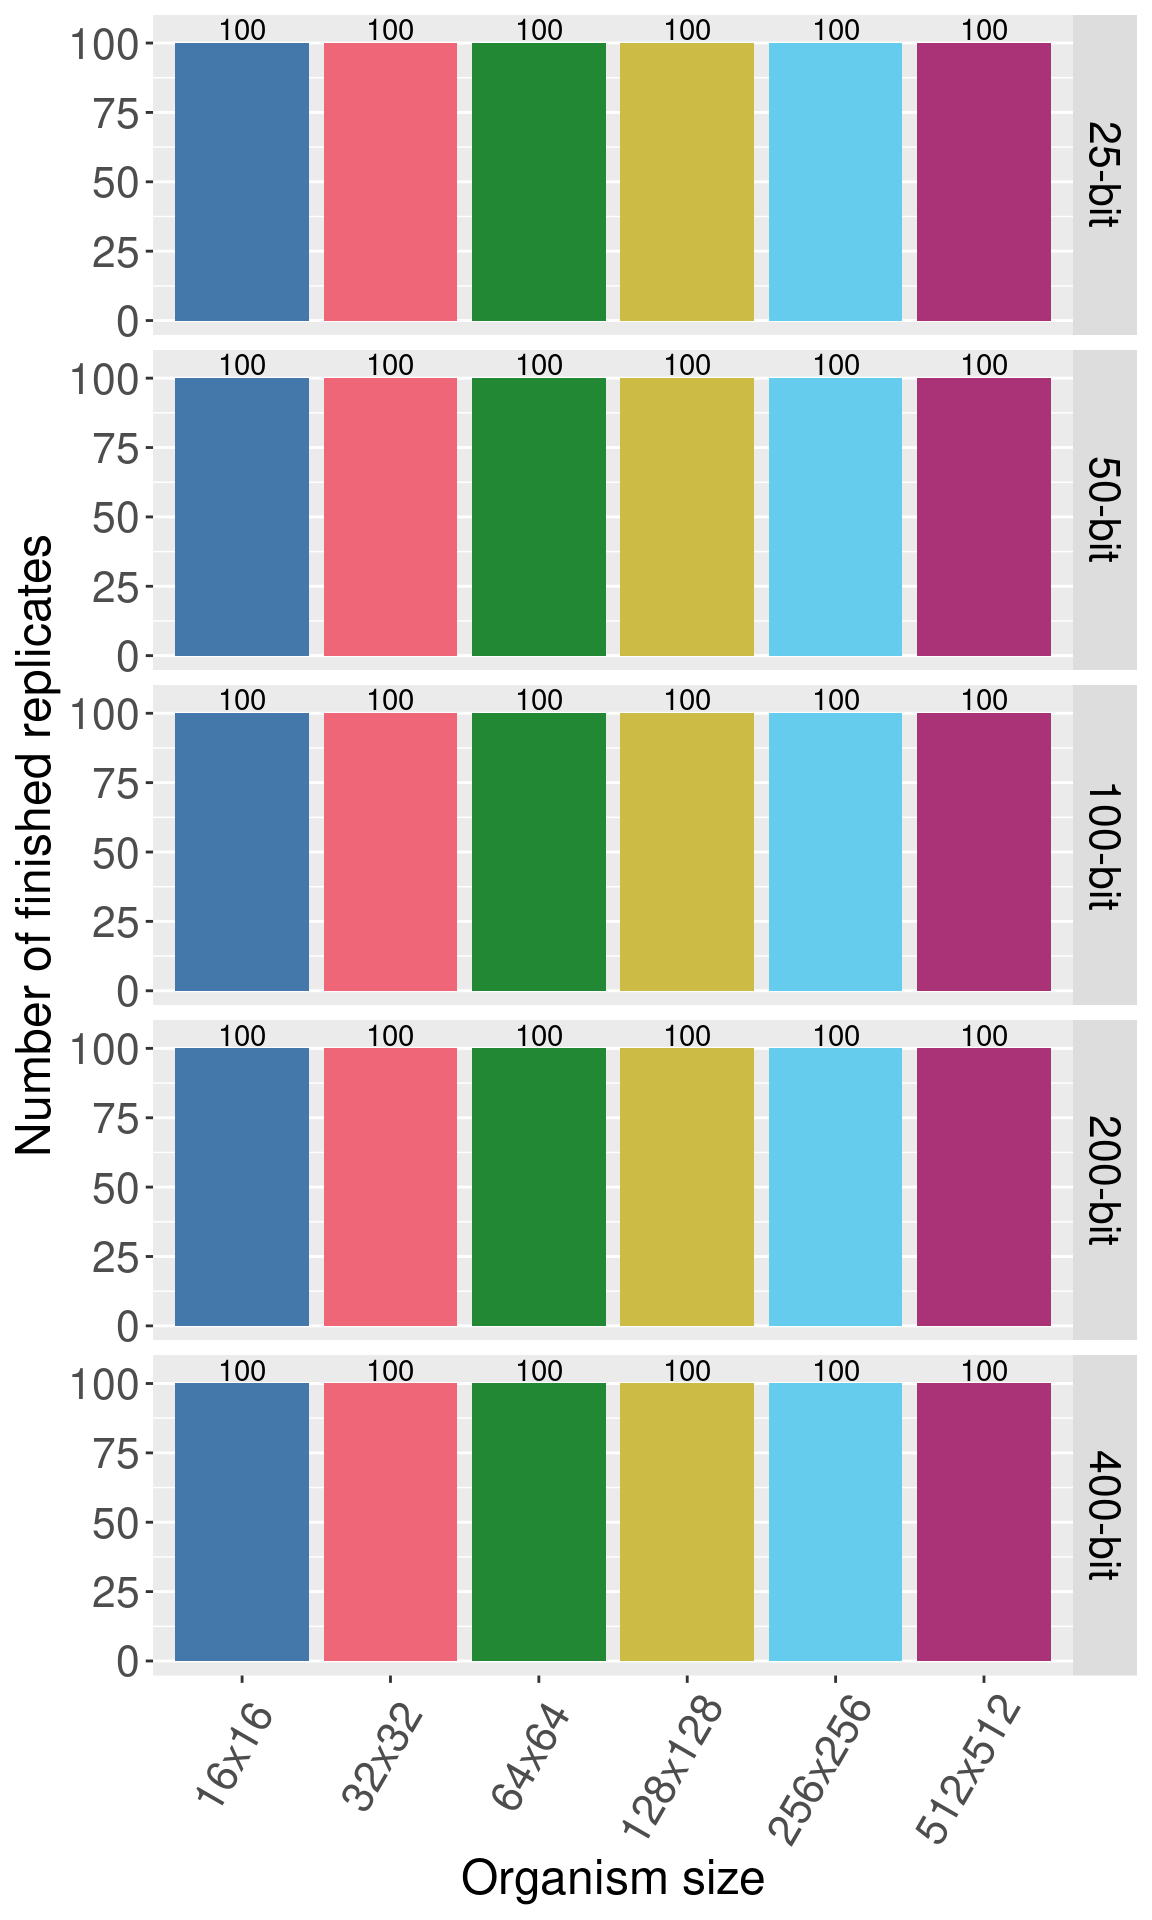
\includegraphics{primordium_supplemental_material_files/figure-latex/unnamed-chunk-62-1.pdf}

\hypertarget{plot}{%
\section{Plot}\label{plot}}

Here we plot all the data.
The figure is split into 6 subplots, each showing a different organism size.
Inside each subplot, the number of timing samples is shown on the x-axis.
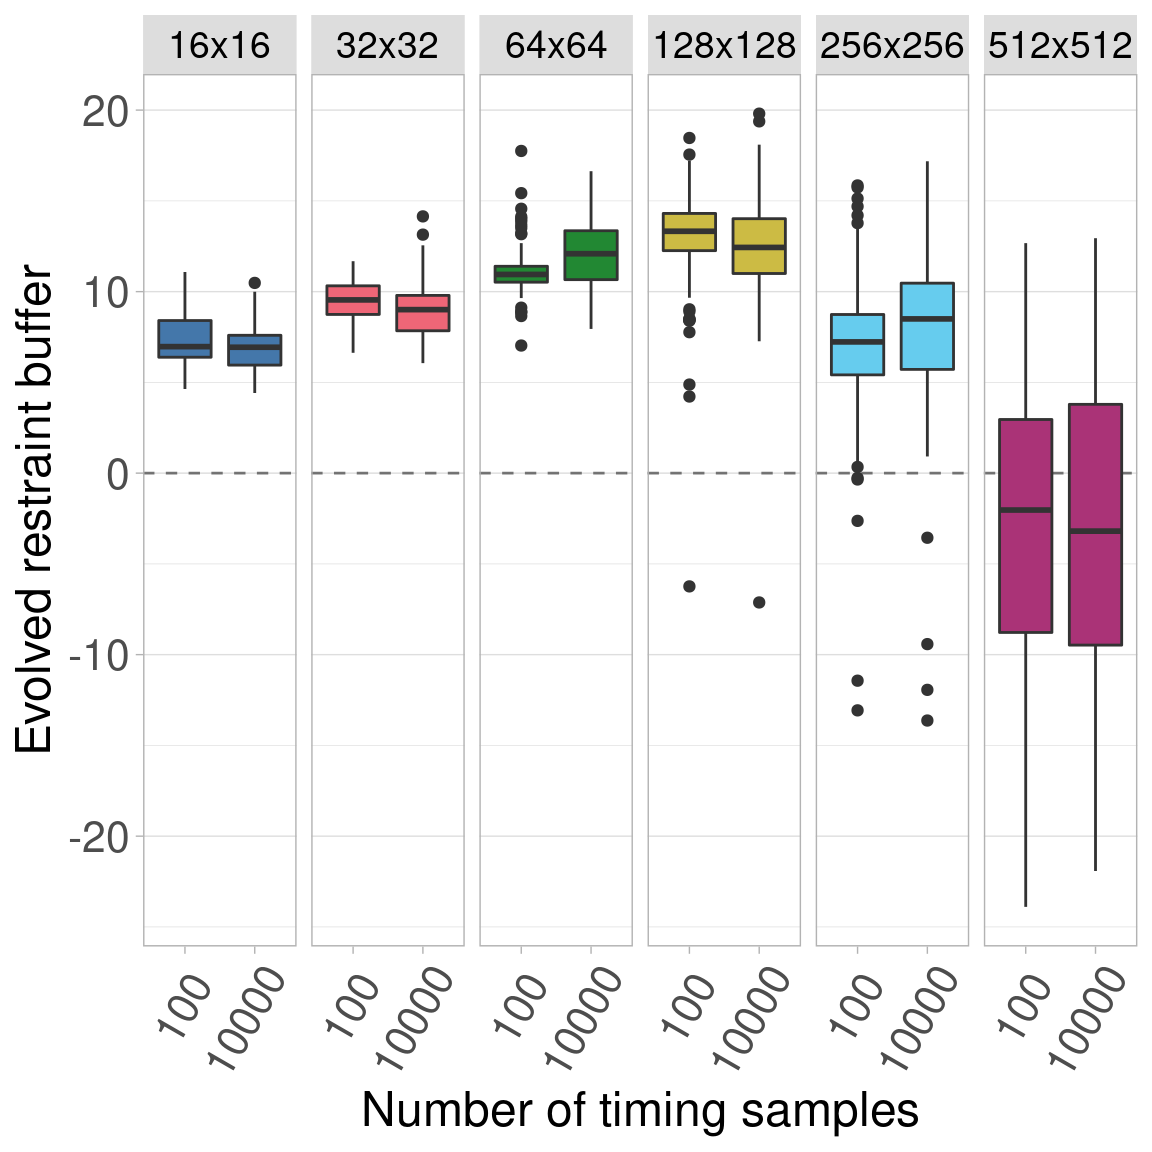
\includegraphics{primordium_supplemental_material_files/figure-latex/unnamed-chunk-63-1.pdf}

\hypertarget{statistics-3}{%
\section{Statistics}\label{statistics-3}}

The plot shows that the general trend, that the evolved restraint buffer initially increases with organism size then decreases, holds true at both sample counts.
Furthermore, we see that the evolved buffer values are fairly consistent between the two sample counts.

While we concluded that this was sufficient evidence to use only 100 samples (10,000 is intractable to run for multiple experiments), we include the statistics here.
Since we treat each organism size as a group, we simply conduct a Wilcoxon Rank-Sum test between 100 samples and 10,000 samples

\begin{verbatim}
##   org_size      p_value      W less_0.01
## 1       16 4.243294e-02 5831.0     FALSE
## 2       32 3.489808e-04 6464.0      TRUE
## 3       64 4.913265e-05 3338.0      TRUE
## 4      128 3.021256e-02 5887.5     FALSE
## 5      256 2.561216e-02 4086.0     FALSE
## 6      512 9.066359e-01 5048.5     FALSE
\end{verbatim}

\hypertarget{population-size-experiment}{%
\chapter{Population size experiment}\label{population-size-experiment}}

By default, all populations contain 200 organisms.
This experiment tested if increasing the population size to 2,000 organisms has any substantial effect on evolved restraint.

This experiment was initially conducted to find our default parameters.
However, the data shown here were reran (with new random number seeds) when we decided to investigate population size in the paper.

The configuration script and data for the experiment can be found under \texttt{2021\_03\_06\_\_pop\_size/} in the experiments directory of the git repository.

\hypertarget{data-cleaning-4}{%
\section{Data cleaning}\label{data-cleaning-4}}

Load necessary libraries

\begin{Shaded}
\begin{Highlighting}[]
\KeywordTok{library}\NormalTok{(dplyr)}
\KeywordTok{library}\NormalTok{(ggplot2)}
\KeywordTok{library}\NormalTok{(ggridges)}
\KeywordTok{library}\NormalTok{(scales)}
\KeywordTok{library}\NormalTok{(khroma)}
\end{Highlighting}
\end{Shaded}

Load the data and trim include only the final generation data for sizes 16x16 to 512x512.

\begin{Shaded}
\begin{Highlighting}[]
\CommentTok{\# Load the data}
\NormalTok{df =}\StringTok{ }\KeywordTok{read.csv}\NormalTok{(}\StringTok{\textquotesingle{}../experiments/2021\_03\_06\_\_pop\_size/evolution/data/scraped\_evolution\_data\_200.csv\textquotesingle{}}\NormalTok{)}
\NormalTok{df =}\StringTok{ }\KeywordTok{rbind}\NormalTok{(df, }\KeywordTok{read.csv}\NormalTok{(}\StringTok{\textquotesingle{}../experiments/2021\_03\_06\_\_pop\_size/evolution/data/scraped\_evolution\_data\_2k.csv\textquotesingle{}}\NormalTok{))}
\CommentTok{\# Trim off NAs (artifacts of how we scraped the data) and trim to only have gen 10,000}
\NormalTok{df2 =}\StringTok{ }\NormalTok{df[}\OperatorTok{!}\KeywordTok{is.na}\NormalTok{(df}\OperatorTok{$}\NormalTok{MCSIZE) }\OperatorTok{\&}\StringTok{ }\NormalTok{df}\OperatorTok{$}\NormalTok{generation }\OperatorTok{==}\StringTok{ }\DecValTok{10000}\NormalTok{,]}
\CommentTok{\# Ignore data for size 8x8 and 1024x1024}
\NormalTok{df2 =}\StringTok{ }\NormalTok{df2[df2}\OperatorTok{$}\NormalTok{MCSIZE }\OperatorTok{!=}\StringTok{ }\DecValTok{8} \OperatorTok{\&}\StringTok{ }\NormalTok{df2}\OperatorTok{$}\NormalTok{MCSIZE }\OperatorTok{!=}\StringTok{ }\DecValTok{1024}\NormalTok{,]}
\end{Highlighting}
\end{Shaded}

We group and summarize the data to ensure all replicates are present.

\begin{Shaded}
\begin{Highlighting}[]
\CommentTok{\# Group the data by size and summarize}
\NormalTok{data\_grouped =}\StringTok{ }\NormalTok{dplyr}\OperatorTok{::}\KeywordTok{group\_by}\NormalTok{(df2, MCSIZE, POP)}
\NormalTok{data\_summary =}\StringTok{ }\NormalTok{dplyr}\OperatorTok{::}\KeywordTok{summarize}\NormalTok{(data\_grouped, }\DataTypeTok{mean\_ones =} \KeywordTok{mean}\NormalTok{(ave\_ones), }\DataTypeTok{n =}\NormalTok{ dplyr}\OperatorTok{::}\KeywordTok{n}\NormalTok{())}
\end{Highlighting}
\end{Shaded}

\begin{verbatim}
## `summarise()` has grouped output by 'MCSIZE'. You can override using the `.groups` argument.
\end{verbatim}

We clean the data and create a few helper variables to make plotting easier.

\begin{Shaded}
\begin{Highlighting}[]
\CommentTok{\# Calculate restraint value (x {-} 60 because genome length is 100 here)}
\NormalTok{df2}\OperatorTok{$}\NormalTok{restraint\_value =}\StringTok{ }\NormalTok{df2}\OperatorTok{$}\NormalTok{ave\_ones }\OperatorTok{{-}}\StringTok{ }\DecValTok{60}
\CommentTok{\# Make a nice, clean factor for size}
\NormalTok{df2}\OperatorTok{$}\NormalTok{size\_str =}\StringTok{ }\KeywordTok{paste0}\NormalTok{(df2}\OperatorTok{$}\NormalTok{MCSIZE, }\StringTok{\textquotesingle{}x\textquotesingle{}}\NormalTok{, df2}\OperatorTok{$}\NormalTok{MCSIZE)}
\NormalTok{df2}\OperatorTok{$}\NormalTok{size\_factor =}\StringTok{ }\KeywordTok{factor}\NormalTok{(df2}\OperatorTok{$}\NormalTok{size\_str, }\DataTypeTok{levels =} \KeywordTok{c}\NormalTok{(}\StringTok{\textquotesingle{}16x16\textquotesingle{}}\NormalTok{, }\StringTok{\textquotesingle{}32x32\textquotesingle{}}\NormalTok{, }\StringTok{\textquotesingle{}64x64\textquotesingle{}}\NormalTok{, }\StringTok{\textquotesingle{}128x128\textquotesingle{}}\NormalTok{, }\StringTok{\textquotesingle{}256x256\textquotesingle{}}\NormalTok{, }\StringTok{\textquotesingle{}512x512\textquotesingle{}}\NormalTok{, }\StringTok{\textquotesingle{}1024x1024\textquotesingle{}}\NormalTok{))}
\NormalTok{df2}\OperatorTok{$}\NormalTok{size\_factor\_reversed =}\StringTok{ }\KeywordTok{factor}\NormalTok{(df2}\OperatorTok{$}\NormalTok{size\_str, }\DataTypeTok{levels =} \KeywordTok{rev}\NormalTok{(}\KeywordTok{c}\NormalTok{(}\StringTok{\textquotesingle{}16x16\textquotesingle{}}\NormalTok{, }\StringTok{\textquotesingle{}32x32\textquotesingle{}}\NormalTok{, }\StringTok{\textquotesingle{}64x64\textquotesingle{}}\NormalTok{, }\StringTok{\textquotesingle{}128x128\textquotesingle{}}\NormalTok{, }\StringTok{\textquotesingle{}256x256\textquotesingle{}}\NormalTok{, }\StringTok{\textquotesingle{}512x512\textquotesingle{}}\NormalTok{, }\StringTok{\textquotesingle{}1024x1024\textquotesingle{}}\NormalTok{)))}
\NormalTok{data\_summary}\OperatorTok{$}\NormalTok{size\_str =}\StringTok{ }\KeywordTok{paste0}\NormalTok{(data\_summary}\OperatorTok{$}\NormalTok{MCSIZE, }\StringTok{\textquotesingle{}x\textquotesingle{}}\NormalTok{, data\_summary}\OperatorTok{$}\NormalTok{MCSIZE)}
\NormalTok{data\_summary}\OperatorTok{$}\NormalTok{size\_factor =}\StringTok{ }\KeywordTok{factor}\NormalTok{(data\_summary}\OperatorTok{$}\NormalTok{size\_str, }\DataTypeTok{levels =} \KeywordTok{c}\NormalTok{(}\StringTok{\textquotesingle{}16x16\textquotesingle{}}\NormalTok{, }\StringTok{\textquotesingle{}32x32\textquotesingle{}}\NormalTok{, }\StringTok{\textquotesingle{}64x64\textquotesingle{}}\NormalTok{, }\StringTok{\textquotesingle{}128x128\textquotesingle{}}\NormalTok{, }\StringTok{\textquotesingle{}256x256\textquotesingle{}}\NormalTok{, }\StringTok{\textquotesingle{}512x512\textquotesingle{}}\NormalTok{, }\StringTok{\textquotesingle{}1024x1024\textquotesingle{}}\NormalTok{))}
\CommentTok{\# Create a map of colors we\textquotesingle{}ll use to plot the different organism sizes}
\NormalTok{color\_vec =}\StringTok{ }\KeywordTok{as.character}\NormalTok{(khroma}\OperatorTok{::}\KeywordTok{color}\NormalTok{(}\StringTok{\textquotesingle{}bright\textquotesingle{}}\NormalTok{)(}\DecValTok{7}\NormalTok{))}
\NormalTok{color\_map =}\StringTok{ }\KeywordTok{c}\NormalTok{(}
  \StringTok{\textquotesingle{}16x16\textquotesingle{}}\NormalTok{ =}\StringTok{     }\NormalTok{color\_vec[}\DecValTok{1}\NormalTok{],}
  \StringTok{\textquotesingle{}32x32\textquotesingle{}}\NormalTok{ =}\StringTok{     }\NormalTok{color\_vec[}\DecValTok{2}\NormalTok{],}
  \StringTok{\textquotesingle{}64x64\textquotesingle{}}\NormalTok{ =}\StringTok{     }\NormalTok{color\_vec[}\DecValTok{3}\NormalTok{],}
  \StringTok{\textquotesingle{}128x128\textquotesingle{}}\NormalTok{ =}\StringTok{   }\NormalTok{color\_vec[}\DecValTok{4}\NormalTok{],}
  \StringTok{\textquotesingle{}256x256\textquotesingle{}}\NormalTok{ =}\StringTok{   }\NormalTok{color\_vec[}\DecValTok{5}\NormalTok{],}
  \StringTok{\textquotesingle{}512x512\textquotesingle{}}\NormalTok{ =}\StringTok{   }\NormalTok{color\_vec[}\DecValTok{6}\NormalTok{],}
  \StringTok{\textquotesingle{}1024x1024\textquotesingle{}}\NormalTok{ =}\StringTok{ }\NormalTok{color\_vec[}\DecValTok{7}\NormalTok{]}
\NormalTok{)}
\CommentTok{\# Set the sizes for text in plots}
\NormalTok{text\_major\_size =}\StringTok{ }\DecValTok{18}
\NormalTok{text\_minor\_size =}\StringTok{ }\DecValTok{16} 
\end{Highlighting}
\end{Shaded}

\hypertarget{data-integrity-check-4}{%
\section{Data integrity check}\label{data-integrity-check-4}}

Now we plot the number of finished replicates for each treatment to make sure all data are present.
Rows show the number of samples used for fitness.
Each bar/color shows a different organism size.
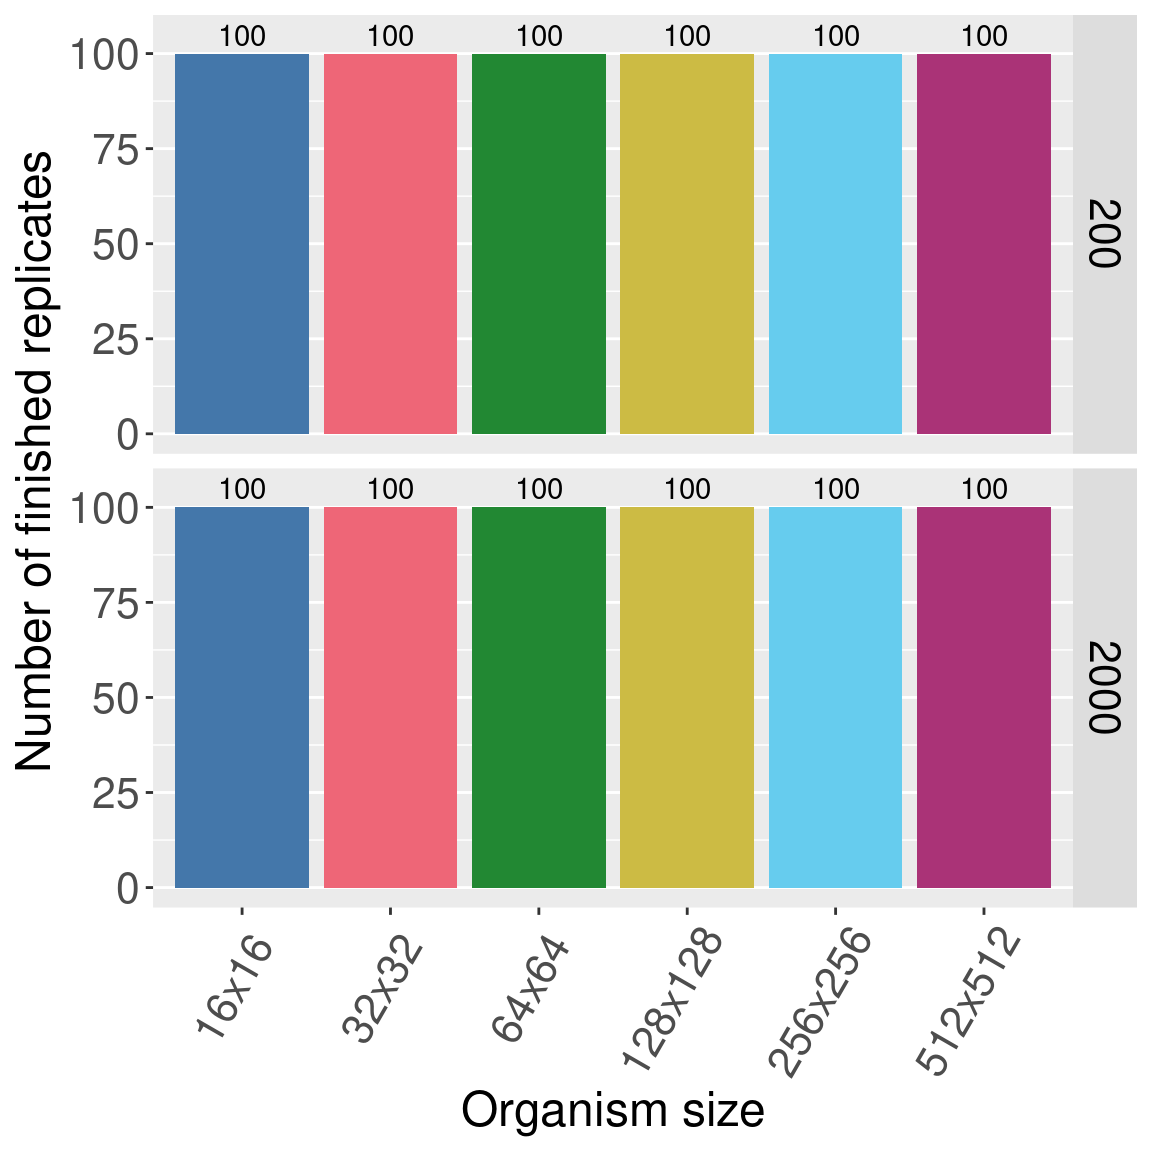
\includegraphics{primordium_supplemental_material_files/figure-latex/unnamed-chunk-69-1.pdf}

\hypertarget{plot-1}{%
\section{Plot}\label{plot-1}}

Here we plot all the data.
The figure is split into 6 subplots, each showing a different organism size.
Inside each subplot, population size is shown on the x-axis.
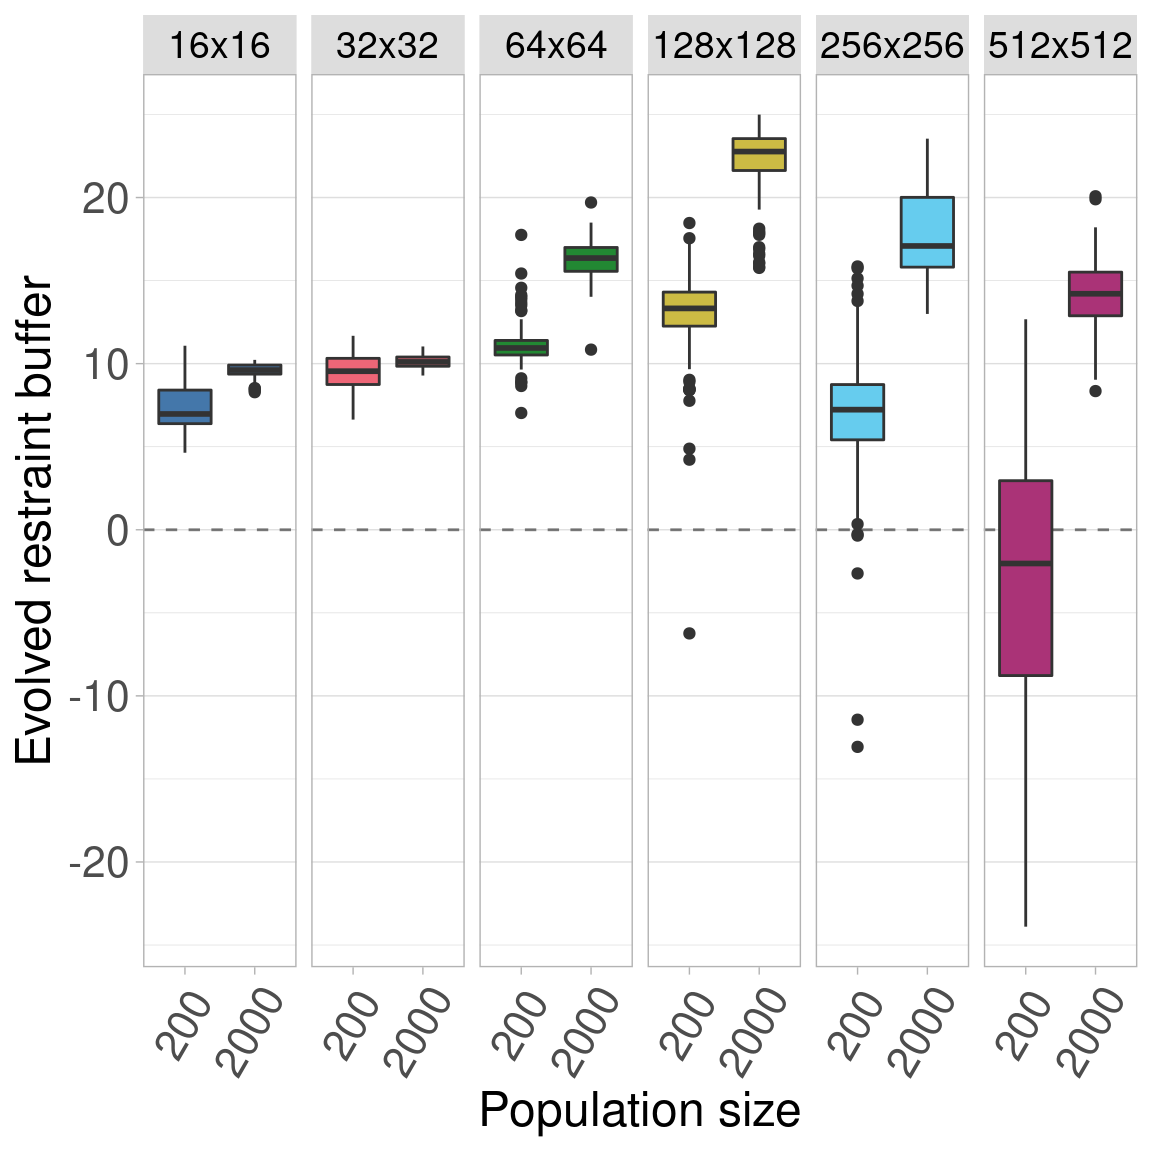
\includegraphics{primordium_supplemental_material_files/figure-latex/unnamed-chunk-70-1.pdf}

\hypertarget{statistics-4}{%
\section{Statistics}\label{statistics-4}}

The plot shows that increasing population size increases the evolved restraint buffer at organism sizes.
Further, we see that the same general trend holds at both population sizes, that evolved restraint peaks at size 128x128.

Finally, we treat each organism size as a group and conduct a Wilcoxon Rank-Sum test between the population sizes.

\begin{verbatim}
##   org_size      p_value      W less_0.01
## 1       16 3.921812e-19 1341.0      TRUE
## 2       32 8.416553e-06 3176.5      TRUE
## 3       64 4.238745e-32  173.0      TRUE
## 4      128 1.013881e-33   46.0      TRUE
## 5      256 2.781080e-33   80.0      TRUE
## 6      512 4.954199e-34   22.0      TRUE
\end{verbatim}

\hypertarget{genome-length-sweep}{%
\chapter{Genome Length Sweep}\label{genome-length-sweep}}

By default, all genomes are bitstrings with 100 bits.
Here, we look into the effects of varying this genome length using lengths of 25, 50, 100, 200, and 400 bits.
Regardless of genome length, the restraint threshold was set at 60\% of the genome being 1s and all organisms started at a restraint buffer of 0.

The configuration script and data for the experiment can be found under \texttt{2021\_02\_27\_\_genome\_length/} in the experiments directory of the git repository.

\hypertarget{data-cleaning-5}{%
\section{Data cleaning}\label{data-cleaning-5}}

Load necessary libraries

\begin{Shaded}
\begin{Highlighting}[]
\KeywordTok{library}\NormalTok{(dplyr)}
\KeywordTok{library}\NormalTok{(ggplot2)}
\KeywordTok{library}\NormalTok{(ggridges)}
\KeywordTok{library}\NormalTok{(scales)}
\KeywordTok{library}\NormalTok{(khroma)}
\end{Highlighting}
\end{Shaded}

Load the data and trim include only the final generation data for sizes 16x16 to 512x512.

\begin{Shaded}
\begin{Highlighting}[]
\CommentTok{\# Load the data}
\NormalTok{df =}\StringTok{ }\KeywordTok{read.csv}\NormalTok{(}\StringTok{\textquotesingle{}../experiments/2021\_02\_27\_\_genome\_length/evolution/data/scraped\_evolution\_data\_length\_50.csv\textquotesingle{}}\NormalTok{)}
\NormalTok{df =}\StringTok{ }\KeywordTok{rbind}\NormalTok{(df, }\KeywordTok{read.csv}\NormalTok{(}\StringTok{\textquotesingle{}../experiments/2021\_02\_27\_\_genome\_length/evolution/data/scraped\_evolution\_data\_length\_200.csv\textquotesingle{}}\NormalTok{))}
\NormalTok{df =}\StringTok{ }\KeywordTok{rbind}\NormalTok{(df, }\KeywordTok{read.csv}\NormalTok{(}\StringTok{\textquotesingle{}../experiments/2021\_02\_27\_\_genome\_length/evolution/data/scraped\_evolution\_data\_length\_100.csv\textquotesingle{}}\NormalTok{))}
\NormalTok{df =}\StringTok{ }\KeywordTok{rbind}\NormalTok{(df, }\KeywordTok{read.csv}\NormalTok{(}\StringTok{\textquotesingle{}../experiments/2021\_02\_27\_\_genome\_length/evolution/data/scraped\_evolution\_data\_length\_400.csv\textquotesingle{}}\NormalTok{))}
\NormalTok{df =}\StringTok{ }\KeywordTok{rbind}\NormalTok{(df, }\KeywordTok{read.csv}\NormalTok{(}\StringTok{\textquotesingle{}../experiments/2021\_02\_27\_\_genome\_length/evolution/data/scraped\_evolution\_data\_length\_25.csv\textquotesingle{}}\NormalTok{))}
\CommentTok{\# Trim off NAs (artifacts of how we scraped the data) and trim to only have gen 10,000}
\NormalTok{df2 =}\StringTok{ }\NormalTok{df[}\OperatorTok{!}\KeywordTok{is.na}\NormalTok{(df}\OperatorTok{$}\NormalTok{MCSIZE) }\OperatorTok{\&}\StringTok{ }\NormalTok{df}\OperatorTok{$}\NormalTok{generation }\OperatorTok{==}\StringTok{ }\DecValTok{10000}\NormalTok{,]}
\CommentTok{\# Ignore data for size 8x8 and 1024x1024}
\NormalTok{df2 =}\StringTok{ }\NormalTok{df2[df2}\OperatorTok{$}\NormalTok{MCSIZE }\OperatorTok{!=}\StringTok{ }\DecValTok{8} \OperatorTok{\&}\StringTok{ }\NormalTok{df2}\OperatorTok{$}\NormalTok{MCSIZE }\OperatorTok{!=}\StringTok{ }\DecValTok{1024}\NormalTok{,]}
\end{Highlighting}
\end{Shaded}

We group and summarize the data to ensure all replicates are present.

\begin{Shaded}
\begin{Highlighting}[]
\CommentTok{\# Group the data by size and summarize}
\NormalTok{data\_grouped =}\StringTok{ }\NormalTok{dplyr}\OperatorTok{::}\KeywordTok{group\_by}\NormalTok{(df2, MCSIZE, LENGTH)}
\NormalTok{data\_summary =}\StringTok{ }\NormalTok{dplyr}\OperatorTok{::}\KeywordTok{summarize}\NormalTok{(data\_grouped, }\DataTypeTok{mean\_ones =} \KeywordTok{mean}\NormalTok{(ave\_ones), }\DataTypeTok{n =}\NormalTok{ dplyr}\OperatorTok{::}\KeywordTok{n}\NormalTok{())}
\end{Highlighting}
\end{Shaded}

\begin{verbatim}
## `summarise()` has grouped output by 'MCSIZE'. You can override using the `.groups` argument.
\end{verbatim}

We clean the data and create a few helper variables to make plotting easier.

\begin{Shaded}
\begin{Highlighting}[]
\CommentTok{\#\# Set variables to make plotting easier}
\CommentTok{\# Calculate restraint value (x {-} 60\% of the genome length)}
\NormalTok{df2}\OperatorTok{$}\NormalTok{restraint\_value =}\StringTok{ }\NormalTok{df2}\OperatorTok{$}\NormalTok{ave\_ones }\OperatorTok{{-}}\StringTok{ }\NormalTok{(df2}\OperatorTok{$}\NormalTok{LENGTH }\OperatorTok{*}\StringTok{ }\FloatTok{0.6}\NormalTok{)}
\CommentTok{\# Make a nice, clean factor for size}
\NormalTok{df2}\OperatorTok{$}\NormalTok{size\_str =}\StringTok{ }\KeywordTok{paste0}\NormalTok{(df2}\OperatorTok{$}\NormalTok{MCSIZE, }\StringTok{\textquotesingle{}x\textquotesingle{}}\NormalTok{, df2}\OperatorTok{$}\NormalTok{MCSIZE)}
\NormalTok{df2}\OperatorTok{$}\NormalTok{size\_factor =}\StringTok{ }\KeywordTok{factor}\NormalTok{(df2}\OperatorTok{$}\NormalTok{size\_str, }\DataTypeTok{levels =} \KeywordTok{c}\NormalTok{(}\StringTok{\textquotesingle{}16x16\textquotesingle{}}\NormalTok{, }\StringTok{\textquotesingle{}32x32\textquotesingle{}}\NormalTok{, }\StringTok{\textquotesingle{}64x64\textquotesingle{}}\NormalTok{, }\StringTok{\textquotesingle{}128x128\textquotesingle{}}\NormalTok{, }\StringTok{\textquotesingle{}256x256\textquotesingle{}}\NormalTok{, }\StringTok{\textquotesingle{}512x512\textquotesingle{}}\NormalTok{, }\StringTok{\textquotesingle{}1024x1024\textquotesingle{}}\NormalTok{))}
\NormalTok{df2}\OperatorTok{$}\NormalTok{size\_factor\_reversed =}\StringTok{ }\KeywordTok{factor}\NormalTok{(df2}\OperatorTok{$}\NormalTok{size\_str, }\DataTypeTok{levels =} \KeywordTok{rev}\NormalTok{(}\KeywordTok{c}\NormalTok{(}\StringTok{\textquotesingle{}16x16\textquotesingle{}}\NormalTok{, }\StringTok{\textquotesingle{}32x32\textquotesingle{}}\NormalTok{, }\StringTok{\textquotesingle{}64x64\textquotesingle{}}\NormalTok{, }\StringTok{\textquotesingle{}128x128\textquotesingle{}}\NormalTok{, }\StringTok{\textquotesingle{}256x256\textquotesingle{}}\NormalTok{, }\StringTok{\textquotesingle{}512x512\textquotesingle{}}\NormalTok{, }\StringTok{\textquotesingle{}1024x1024\textquotesingle{}}\NormalTok{)))}
\NormalTok{df2}\OperatorTok{$}\NormalTok{length\_str =}\StringTok{ }\KeywordTok{paste0}\NormalTok{(df2}\OperatorTok{$}\NormalTok{LENGTH, }\StringTok{\textquotesingle{}{-}bit\textquotesingle{}}\NormalTok{)}
\NormalTok{df2}\OperatorTok{$}\NormalTok{length\_factor =}\StringTok{ }\KeywordTok{factor}\NormalTok{(df2}\OperatorTok{$}\NormalTok{length\_str, }\DataTypeTok{levels =} \KeywordTok{c}\NormalTok{(}\StringTok{\textquotesingle{}25{-}bit\textquotesingle{}}\NormalTok{, }\StringTok{\textquotesingle{}50{-}bit\textquotesingle{}}\NormalTok{, }\StringTok{\textquotesingle{}100{-}bit\textquotesingle{}}\NormalTok{, }\StringTok{\textquotesingle{}200{-}bit\textquotesingle{}}\NormalTok{, }\StringTok{\textquotesingle{}400{-}bit\textquotesingle{}}\NormalTok{))}
\NormalTok{data\_summary}\OperatorTok{$}\NormalTok{size\_str =}\StringTok{ }\KeywordTok{paste0}\NormalTok{(data\_summary}\OperatorTok{$}\NormalTok{MCSIZE, }\StringTok{\textquotesingle{}x\textquotesingle{}}\NormalTok{, data\_summary}\OperatorTok{$}\NormalTok{MCSIZE)}
\NormalTok{data\_summary}\OperatorTok{$}\NormalTok{size\_factor =}\StringTok{ }\KeywordTok{factor}\NormalTok{(data\_summary}\OperatorTok{$}\NormalTok{size\_str, }\DataTypeTok{levels =} \KeywordTok{c}\NormalTok{(}\StringTok{\textquotesingle{}16x16\textquotesingle{}}\NormalTok{, }\StringTok{\textquotesingle{}32x32\textquotesingle{}}\NormalTok{, }\StringTok{\textquotesingle{}64x64\textquotesingle{}}\NormalTok{, }\StringTok{\textquotesingle{}128x128\textquotesingle{}}\NormalTok{, }\StringTok{\textquotesingle{}256x256\textquotesingle{}}\NormalTok{, }\StringTok{\textquotesingle{}512x512\textquotesingle{}}\NormalTok{, }\StringTok{\textquotesingle{}1024x1024\textquotesingle{}}\NormalTok{))}
\NormalTok{data\_summary}\OperatorTok{$}\NormalTok{length\_str =}\StringTok{ }\KeywordTok{paste0}\NormalTok{(data\_summary}\OperatorTok{$}\NormalTok{LENGTH, }\StringTok{\textquotesingle{}{-}bit\textquotesingle{}}\NormalTok{)}
\NormalTok{data\_summary}\OperatorTok{$}\NormalTok{length\_factor =}\StringTok{ }\KeywordTok{factor}\NormalTok{(data\_summary}\OperatorTok{$}\NormalTok{length\_str, }\DataTypeTok{levels =} \KeywordTok{c}\NormalTok{(}\StringTok{\textquotesingle{}25{-}bit\textquotesingle{}}\NormalTok{, }\StringTok{\textquotesingle{}50{-}bit\textquotesingle{}}\NormalTok{, }\StringTok{\textquotesingle{}100{-}bit\textquotesingle{}}\NormalTok{, }\StringTok{\textquotesingle{}200{-}bit\textquotesingle{}}\NormalTok{, }\StringTok{\textquotesingle{}400{-}bit\textquotesingle{}}\NormalTok{))}
\CommentTok{\# Create a map of colors we\textquotesingle{}ll use to plot the different organism sizes}
\NormalTok{color\_vec =}\StringTok{ }\KeywordTok{as.character}\NormalTok{(khroma}\OperatorTok{::}\KeywordTok{color}\NormalTok{(}\StringTok{\textquotesingle{}bright\textquotesingle{}}\NormalTok{)(}\DecValTok{7}\NormalTok{))}
\NormalTok{color\_map =}\StringTok{ }\KeywordTok{c}\NormalTok{(}
  \StringTok{\textquotesingle{}16x16\textquotesingle{}}\NormalTok{ =}\StringTok{     }\NormalTok{color\_vec[}\DecValTok{1}\NormalTok{],}
  \StringTok{\textquotesingle{}32x32\textquotesingle{}}\NormalTok{ =}\StringTok{     }\NormalTok{color\_vec[}\DecValTok{2}\NormalTok{],}
  \StringTok{\textquotesingle{}64x64\textquotesingle{}}\NormalTok{ =}\StringTok{     }\NormalTok{color\_vec[}\DecValTok{3}\NormalTok{],}
  \StringTok{\textquotesingle{}128x128\textquotesingle{}}\NormalTok{ =}\StringTok{   }\NormalTok{color\_vec[}\DecValTok{4}\NormalTok{],}
  \StringTok{\textquotesingle{}256x256\textquotesingle{}}\NormalTok{ =}\StringTok{   }\NormalTok{color\_vec[}\DecValTok{5}\NormalTok{],}
  \StringTok{\textquotesingle{}512x512\textquotesingle{}}\NormalTok{ =}\StringTok{   }\NormalTok{color\_vec[}\DecValTok{6}\NormalTok{],}
  \StringTok{\textquotesingle{}1024x1024\textquotesingle{}}\NormalTok{ =}\StringTok{ }\NormalTok{color\_vec[}\DecValTok{7}\NormalTok{]}
\NormalTok{)}
\CommentTok{\# Set the sizes for text in plots}
\NormalTok{text\_major\_size =}\StringTok{ }\DecValTok{18}
\NormalTok{text\_minor\_size =}\StringTok{ }\DecValTok{16} 
\end{Highlighting}
\end{Shaded}

\hypertarget{data-integrity-check-5}{%
\section{Data integrity check}\label{data-integrity-check-5}}

Now we plot the number of finished replicates for each treatment to make sure all data are present.
Each row shows a different genome length (in bits).
Each bar/color shows a different organism size.
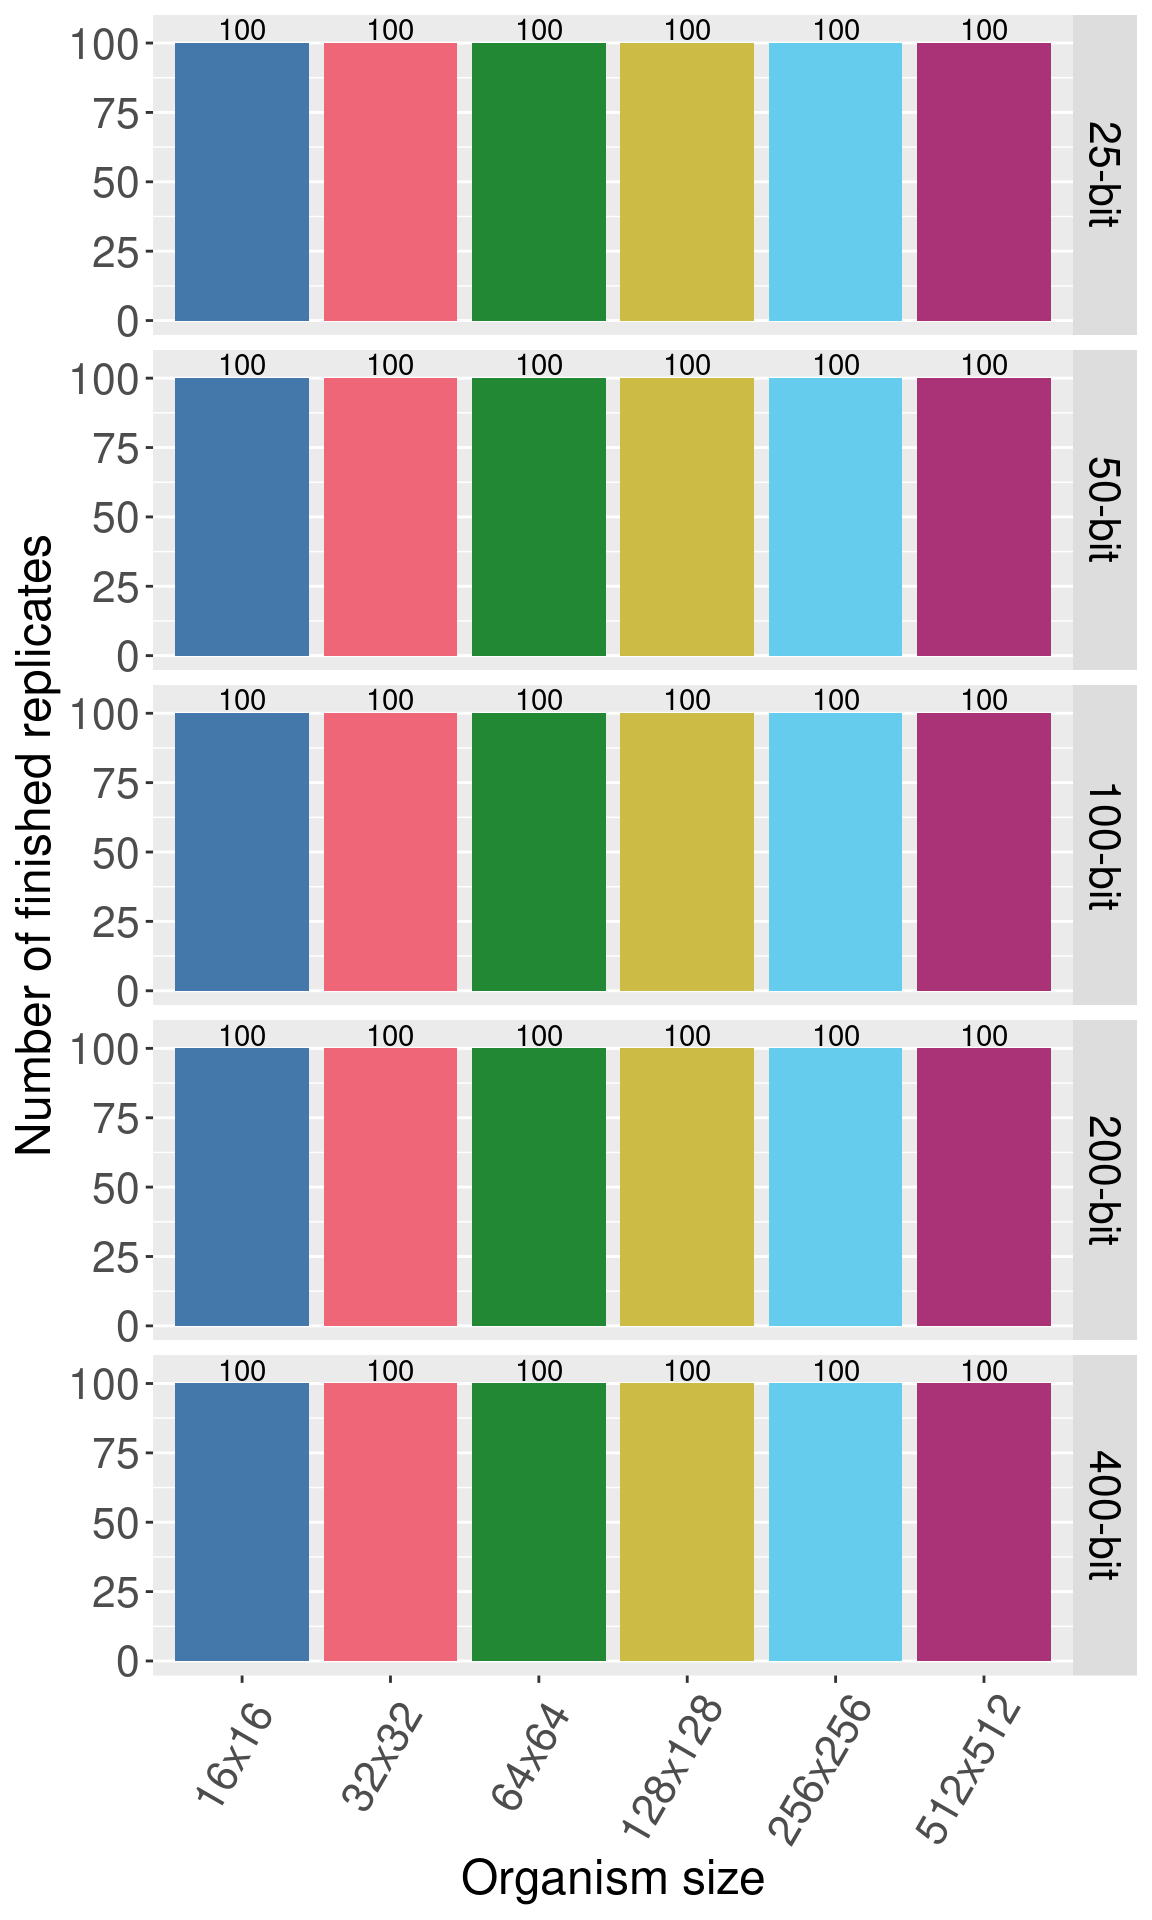
\includegraphics{primordium_supplemental_material_files/figure-latex/unnamed-chunk-76-1.pdf}

\hypertarget{aggregate-plots-3}{%
\section{Aggregate plots}\label{aggregate-plots-3}}

\hypertarget{facet-by-genome-length}{%
\subsection{Facet by genome length}\label{facet-by-genome-length}}

Here we plot all the data at once.
Each row shows a different genome length and each boxplot shows a given organism size.

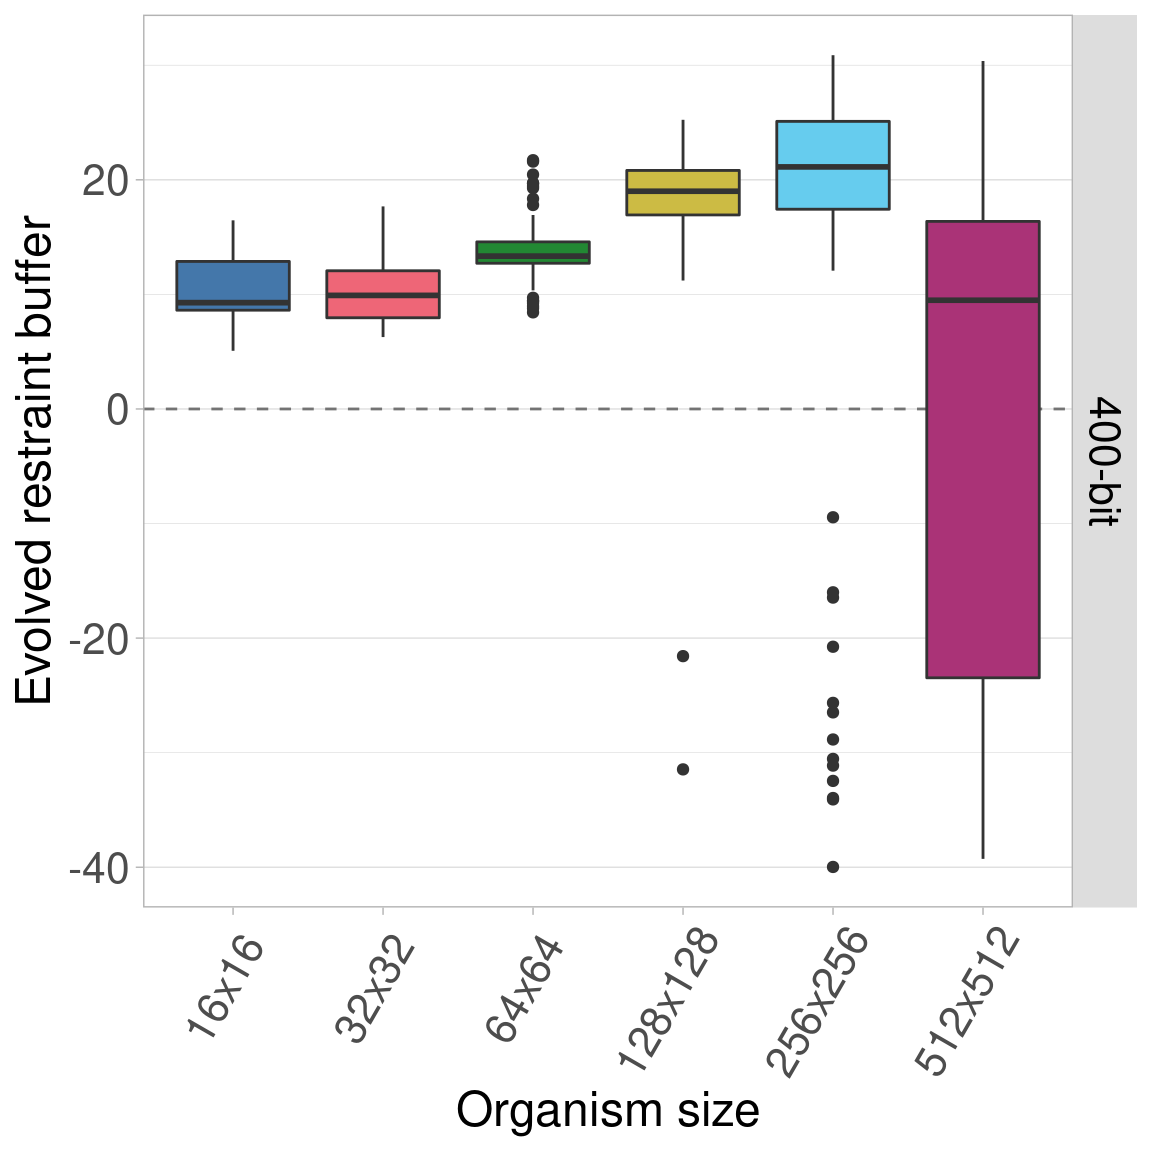
\includegraphics{primordium_supplemental_material_files/figure-latex/unnamed-chunk-77-1.pdf}

Here we plot the same data, only we allow the y-axis to vary between rows.
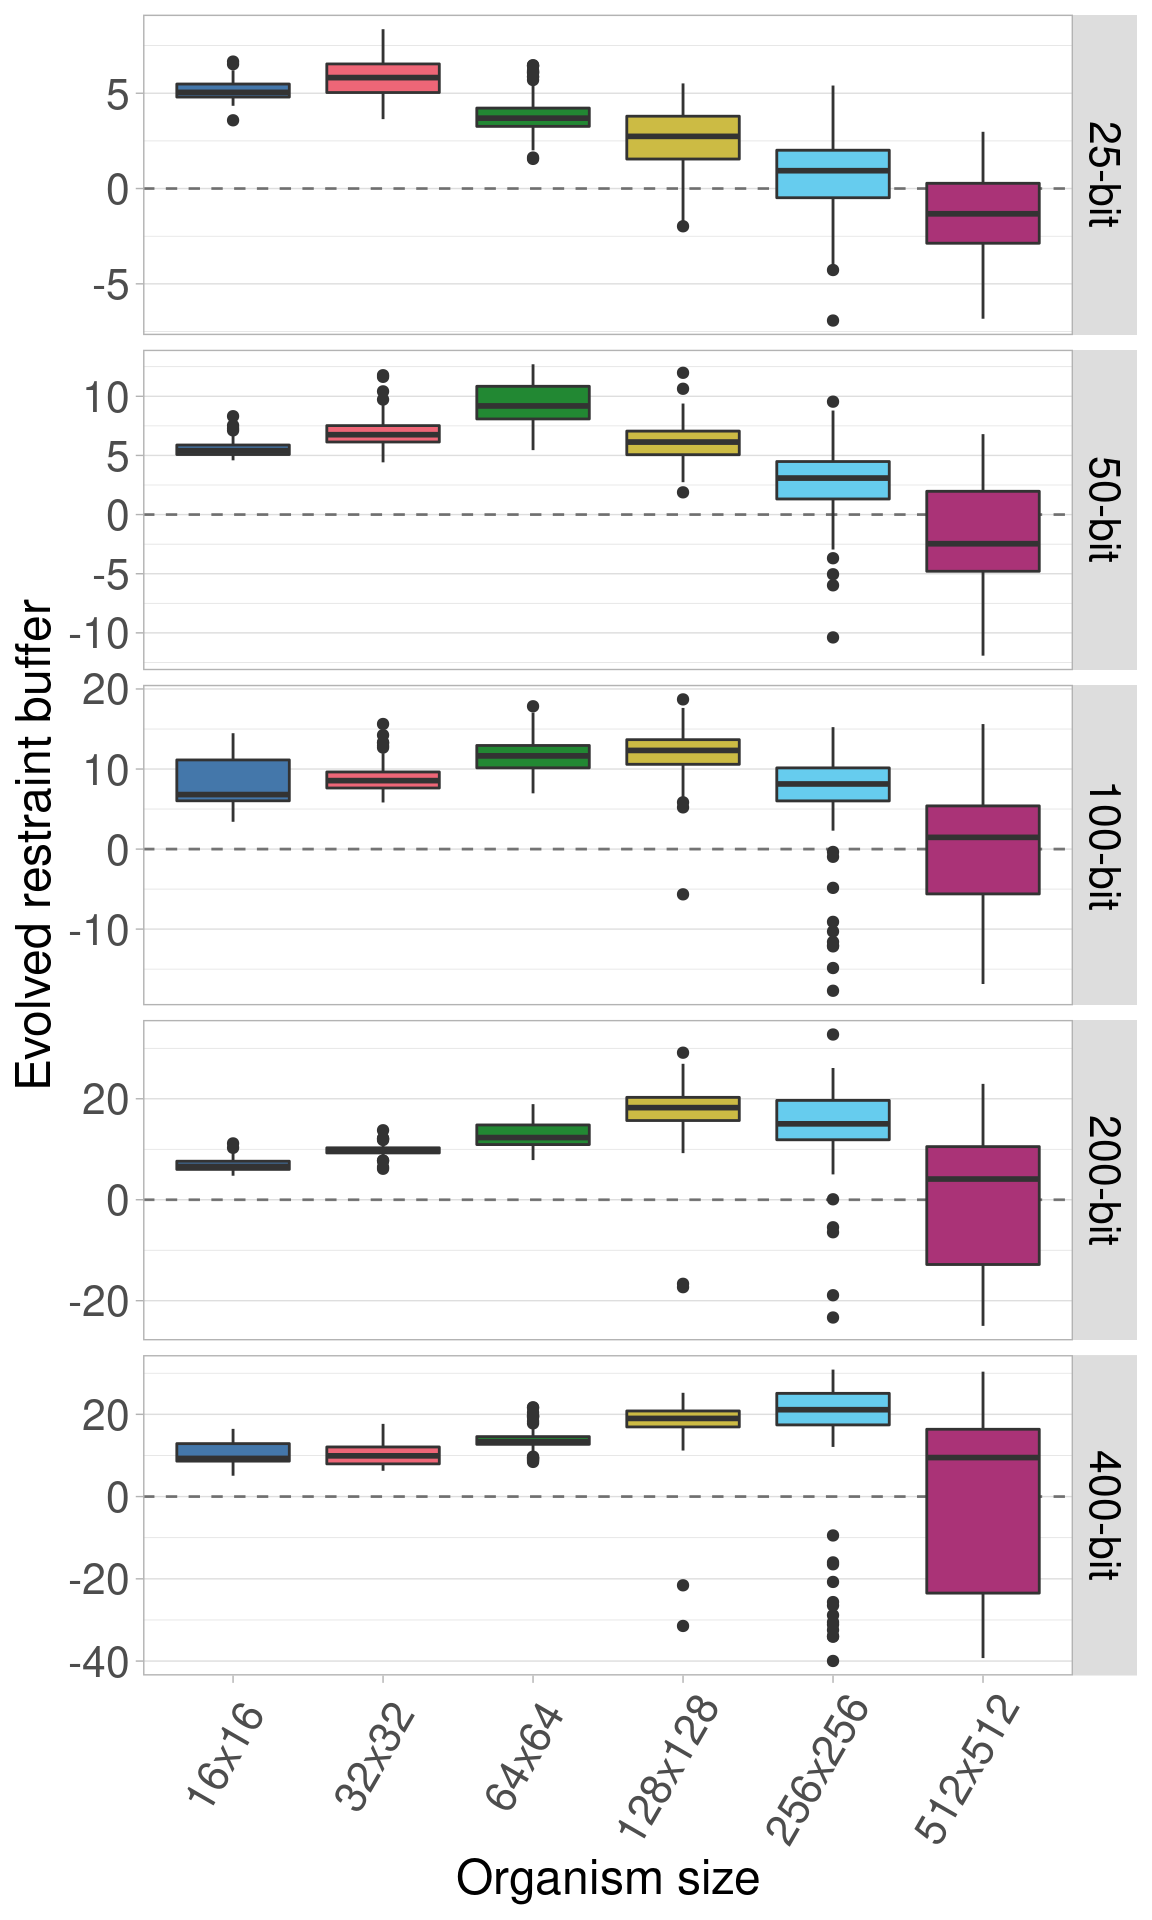
\includegraphics{primordium_supplemental_material_files/figure-latex/unnamed-chunk-78-1.pdf}

\hypertarget{facet-by-organism-size-2}{%
\subsection{Facet by organism size}\label{facet-by-organism-size-2}}

Here we plot the same data again, only now each row shows an organism size while genome length varies on the x-axis.

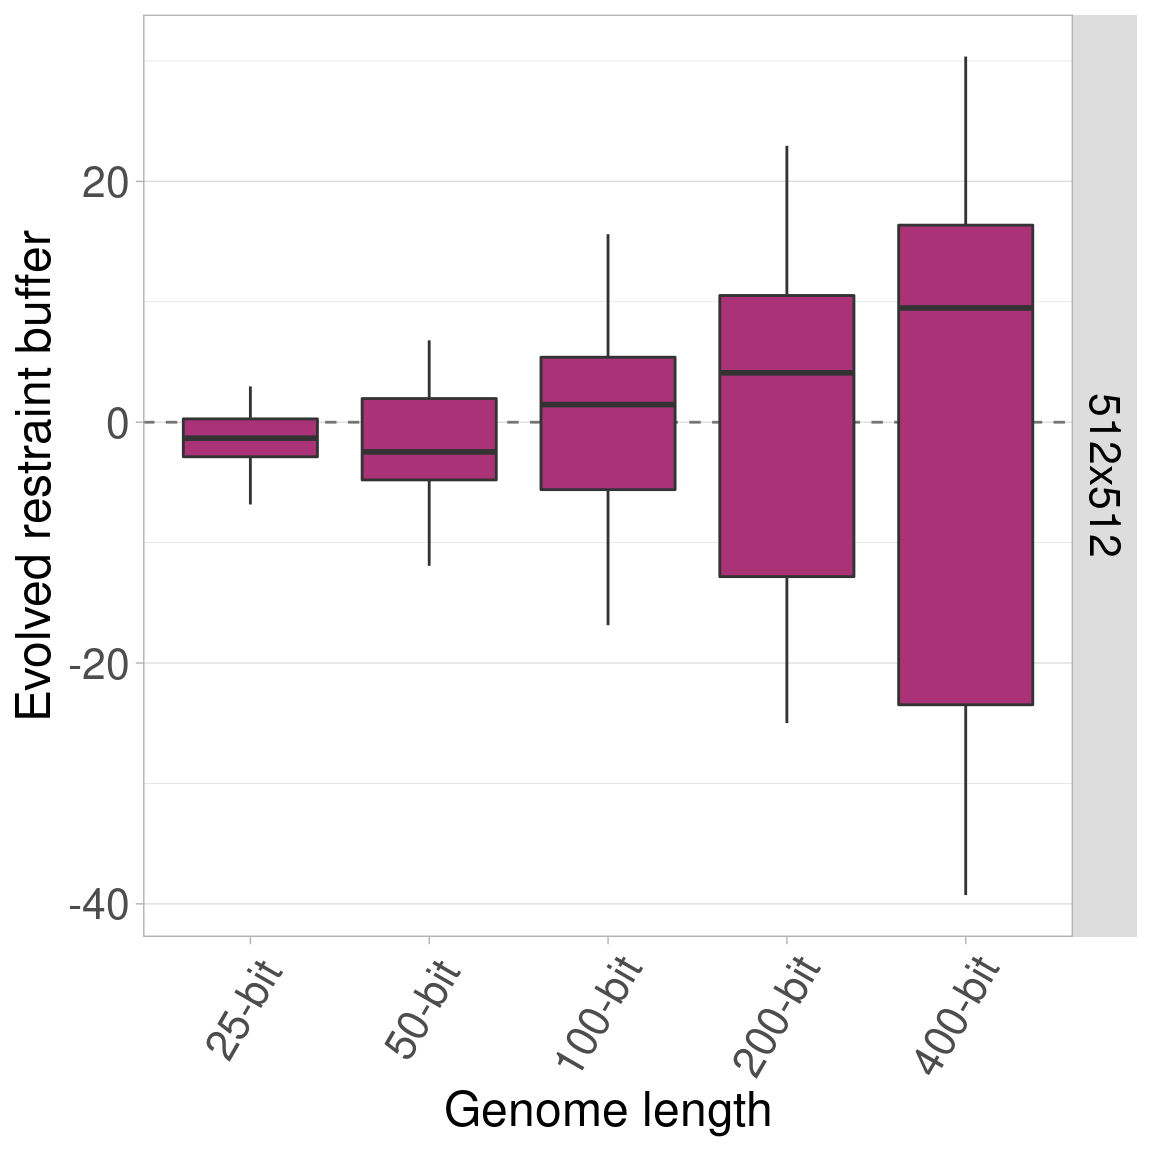
\includegraphics{primordium_supplemental_material_files/figure-latex/unnamed-chunk-79-1.pdf}

Here is the identical plot, but now we allow the y-axis to vary between the rows.

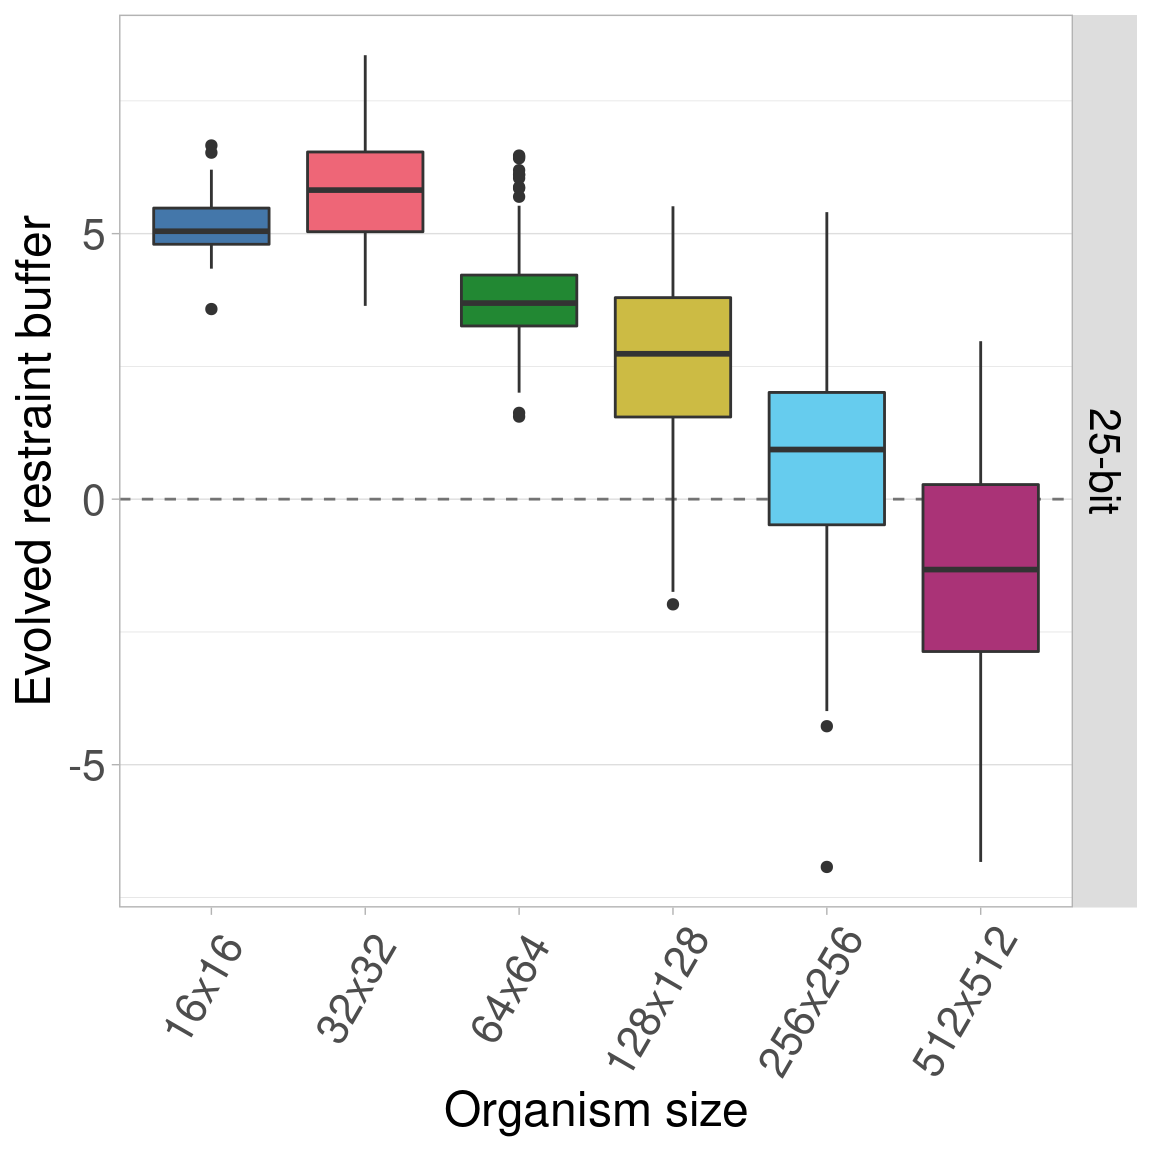
\includegraphics{primordium_supplemental_material_files/figure-latex/unnamed-chunk-80-1.pdf}

\hypertarget{single-organism-size-plots-3}{%
\section{Single organism size plots}\label{single-organism-size-plots-3}}

Here we plot each organism size independently, with the genome length on the x-axis.

\hypertarget{organism-size-16x16-2}{%
\subsection{Organism size 16x16}\label{organism-size-16x16-2}}

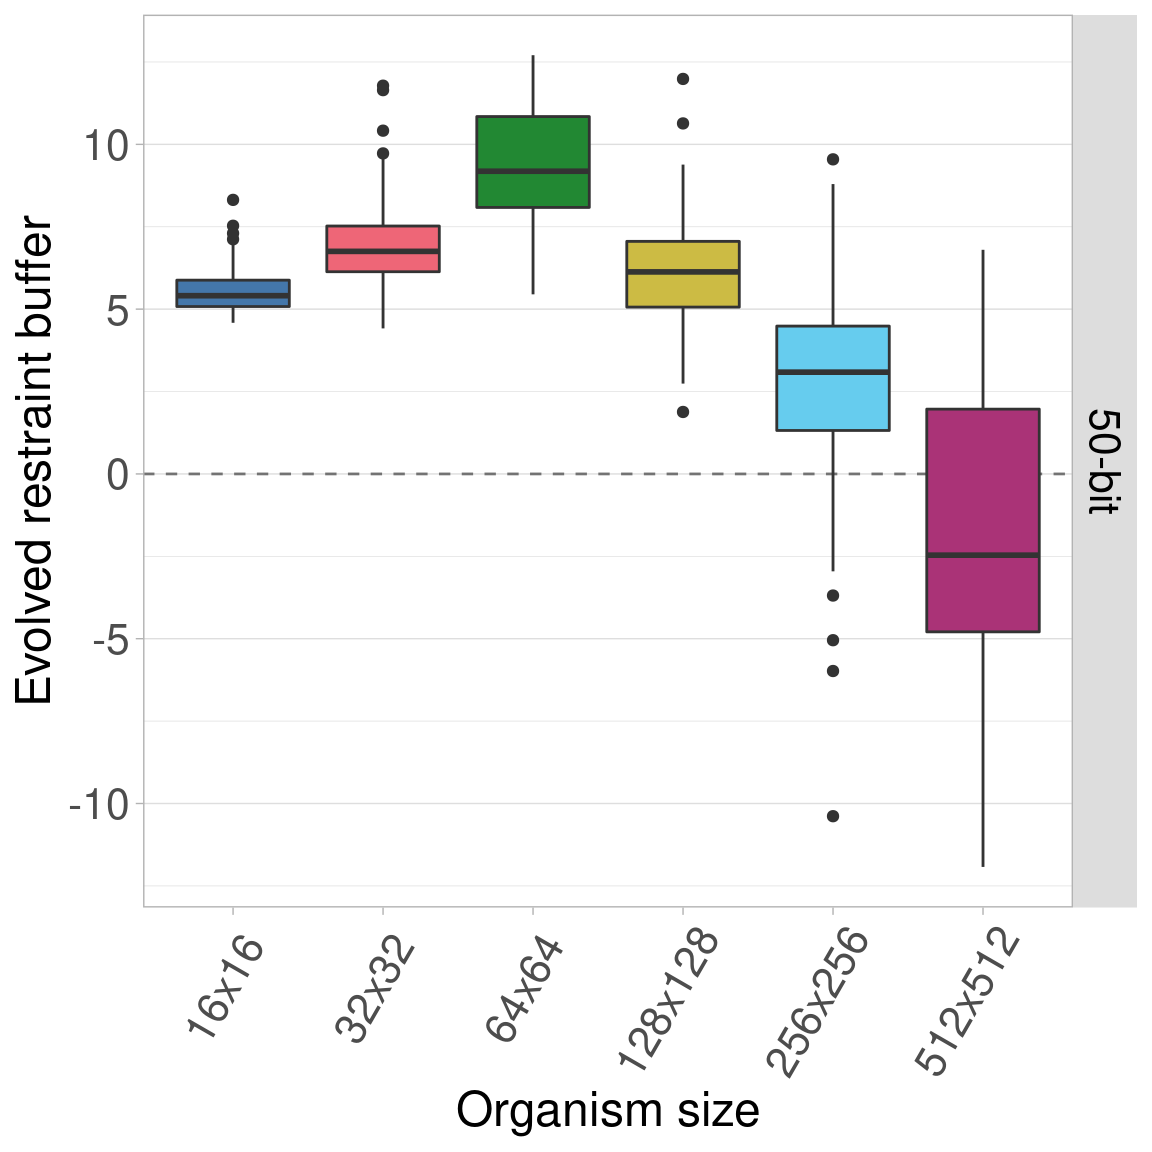
\includegraphics{primordium_supplemental_material_files/figure-latex/unnamed-chunk-81-1.pdf}

\hypertarget{organism-size-32x32-2}{%
\subsection{Organism size 32x32}\label{organism-size-32x32-2}}

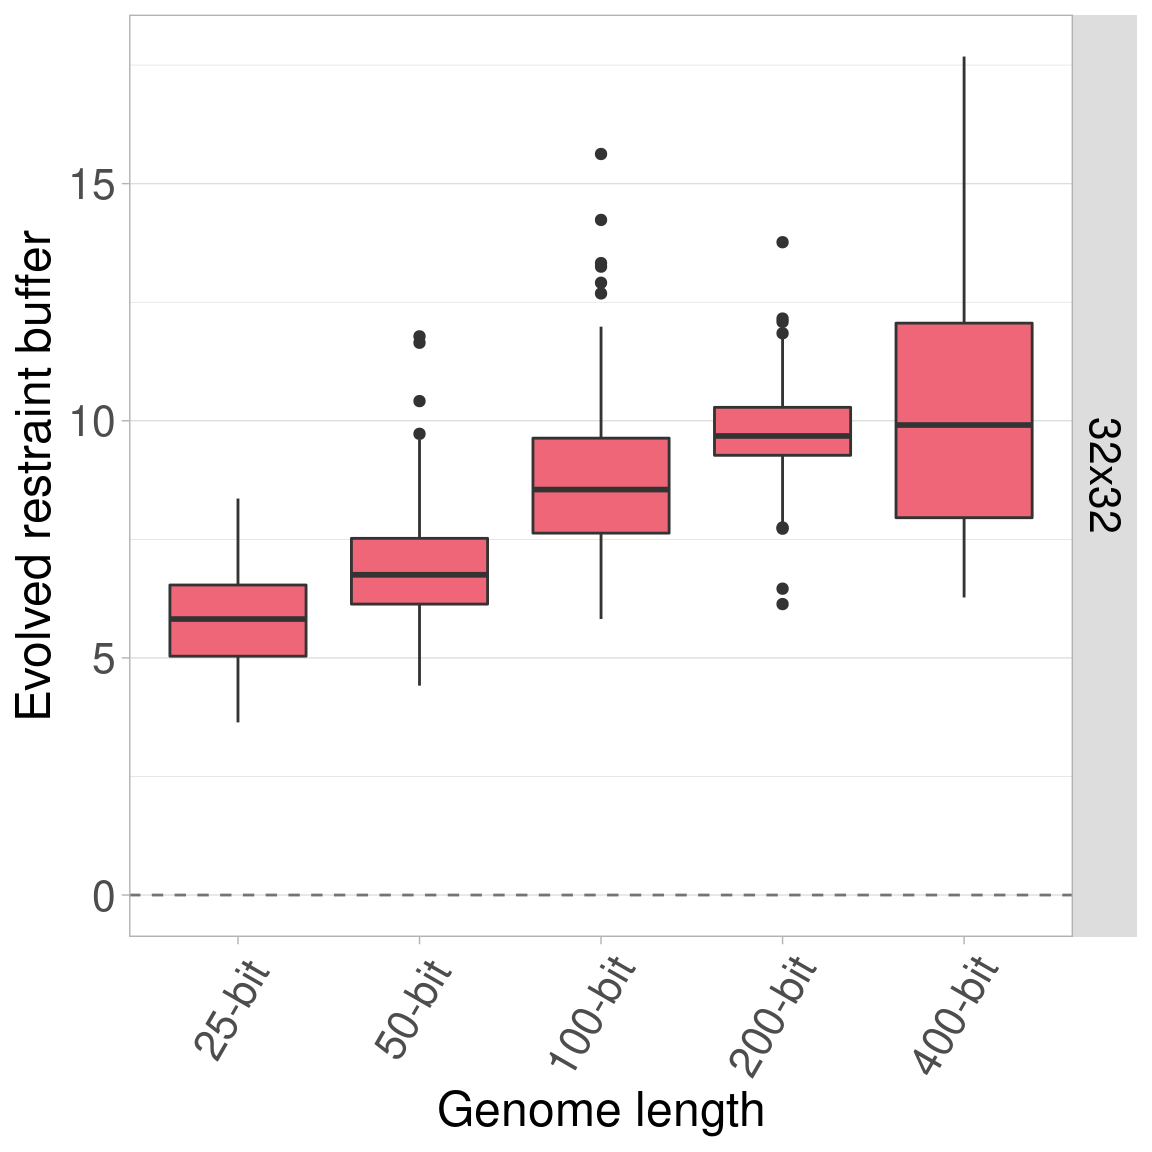
\includegraphics{primordium_supplemental_material_files/figure-latex/unnamed-chunk-82-1.pdf}

\hypertarget{organism-size-64x64-2}{%
\subsection{Organism size 64x64}\label{organism-size-64x64-2}}

\includegraphics{primordium_supplemental_material_files/figure-latex/unnamed-chunk-83-1.pdf}

\hypertarget{organism-size-128x128-2}{%
\subsection{Organism size 128x128}\label{organism-size-128x128-2}}

\includegraphics{primordium_supplemental_material_files/figure-latex/unnamed-chunk-84-1.pdf}

\hypertarget{organism-size-256x256-2}{%
\subsection{Organism size 256x256}\label{organism-size-256x256-2}}

\includegraphics{primordium_supplemental_material_files/figure-latex/unnamed-chunk-85-1.pdf}

\hypertarget{organism-size-512x512-2}{%
\subsection{Organism size 512x512}\label{organism-size-512x512-2}}

\includegraphics{primordium_supplemental_material_files/figure-latex/unnamed-chunk-86-1.pdf}

\hypertarget{single-genome-length-plots}{%
\section{Single genome length plots}\label{single-genome-length-plots}}

Here we plot each genome length independently, with the organism size on the x-axis.

\hypertarget{bit-genomes}{%
\subsection{25-bit genomes}\label{bit-genomes}}

\includegraphics{primordium_supplemental_material_files/figure-latex/unnamed-chunk-87-1.pdf}

\hypertarget{bit-genomes-1}{%
\subsection{50-bit genomes}\label{bit-genomes-1}}

\includegraphics{primordium_supplemental_material_files/figure-latex/unnamed-chunk-88-1.pdf}

\hypertarget{bit-genomes-2}{%
\subsection{100-bit genomes}\label{bit-genomes-2}}

\includegraphics{primordium_supplemental_material_files/figure-latex/unnamed-chunk-89-1.pdf}

\hypertarget{bit-genomes-3}{%
\subsection{200-bit genomes}\label{bit-genomes-3}}

\includegraphics{primordium_supplemental_material_files/figure-latex/unnamed-chunk-90-1.pdf}

\hypertarget{bit-genomes-4}{%
\subsection{400-bit genomes}\label{bit-genomes-4}}

\includegraphics{primordium_supplemental_material_files/figure-latex/unnamed-chunk-91-1.pdf}

\hypertarget{statistics-5}{%
\section{Statistics}\label{statistics-5}}

Since organism size is our main point of comparison, we calculate statistics for each genome length.

First, we perform a Kruskal-Wallis test across all organism sizes to indicate if variance exists at that mutation rate.
If variance exists, we then perform a pairwise Wilcoxon Rank-Sum test to show which pairs of organism sizes significantly differ.
Finally, we perform Bonferroni-Holm corrections for multiple comparisons.

\begin{Shaded}
\begin{Highlighting}[]
\NormalTok{  length\_vec =}\StringTok{ }\KeywordTok{c}\NormalTok{(}\DecValTok{25}\NormalTok{, }\DecValTok{50}\NormalTok{, }\DecValTok{100}\NormalTok{, }\DecValTok{200}\NormalTok{, }\DecValTok{400}\NormalTok{)}
\NormalTok{  df\_kruskal =}\StringTok{ }\KeywordTok{data.frame}\NormalTok{(}\DataTypeTok{data =} \KeywordTok{matrix}\NormalTok{(}\DataTypeTok{nrow =} \DecValTok{0}\NormalTok{, }\DataTypeTok{ncol =} \DecValTok{4}\NormalTok{))}
  \KeywordTok{colnames}\NormalTok{(df\_kruskal) =}\StringTok{ }\KeywordTok{c}\NormalTok{(}\StringTok{\textquotesingle{}genome\_length\textquotesingle{}}\NormalTok{, }\StringTok{\textquotesingle{}p\_value\textquotesingle{}}\NormalTok{, }\StringTok{\textquotesingle{}chi\_squared\textquotesingle{}}\NormalTok{, }\StringTok{\textquotesingle{}df\textquotesingle{}}\NormalTok{)}
  \ControlFlowTok{for}\NormalTok{(genome\_length }\ControlFlowTok{in}\NormalTok{ length\_vec)\{}
\NormalTok{    df\_test =}\StringTok{ }\NormalTok{df2[df2}\OperatorTok{$}\NormalTok{LENGTH }\OperatorTok{==}\StringTok{ }\NormalTok{genome\_length,]}
\NormalTok{    res =}\StringTok{ }\KeywordTok{kruskal.test}\NormalTok{(df\_test}\OperatorTok{$}\NormalTok{restraint\_value }\OperatorTok{\textasciitilde{}}\StringTok{ }\NormalTok{df\_test}\OperatorTok{$}\NormalTok{MCSIZE, df\_test)}
\NormalTok{    df\_kruskal[}\KeywordTok{nrow}\NormalTok{(df\_kruskal) }\OperatorTok{+}\StringTok{ }\DecValTok{1}\NormalTok{,] =}\StringTok{ }\KeywordTok{c}\NormalTok{(genome\_length, res}\OperatorTok{$}\NormalTok{p.value, }\KeywordTok{as.numeric}\NormalTok{(res}\OperatorTok{$}\NormalTok{statistic)[}\DecValTok{1}\NormalTok{], }\KeywordTok{as.numeric}\NormalTok{(res}\OperatorTok{$}\NormalTok{parameter)[}\DecValTok{1}\NormalTok{])}
\NormalTok{  \}}
\NormalTok{  df\_kruskal}\OperatorTok{$}\NormalTok{less\_}\FloatTok{0.01}\NormalTok{ =}\StringTok{ }\NormalTok{df\_kruskal}\OperatorTok{$}\NormalTok{p\_value }\OperatorTok{\textless{}}\StringTok{ }\FloatTok{0.01}
  \KeywordTok{print}\NormalTok{(df\_kruskal)}
\end{Highlighting}
\end{Shaded}

\begin{verbatim}
##   genome_length      p_value chi_squared df less_0.01
## 1            25 1.508889e-97    461.6473  5      TRUE
## 2            50 9.772852e-87    411.5159  5      TRUE
## 3           100 7.491319e-60    286.6294  5      TRUE
## 4           200 1.626963e-75    359.4358  5      TRUE
## 5           400 2.857912e-49    237.3380  5      TRUE
\end{verbatim}

We see that significant variation exists within each genome length, so we perform pairwise Wilcoxon tests on each to see which pairs of sizes are significantly different.

\begin{Shaded}
\begin{Highlighting}[]
\NormalTok{size\_vec =}\StringTok{ }\KeywordTok{c}\NormalTok{(}\DecValTok{16}\NormalTok{, }\DecValTok{32}\NormalTok{, }\DecValTok{64}\NormalTok{, }\DecValTok{128}\NormalTok{, }\DecValTok{256}\NormalTok{, }\DecValTok{512}\NormalTok{)}
\NormalTok{length\_vec =}\StringTok{ }\KeywordTok{c}\NormalTok{(}\DecValTok{25}\NormalTok{, }\DecValTok{50}\NormalTok{, }\DecValTok{100}\NormalTok{, }\DecValTok{200}\NormalTok{, }\DecValTok{400}\NormalTok{)}
\ControlFlowTok{for}\NormalTok{(genome\_length }\ControlFlowTok{in}\NormalTok{ length\_vec)\{}
\NormalTok{  df\_test =}\StringTok{ }\NormalTok{df2[df2}\OperatorTok{$}\NormalTok{LENGTH }\OperatorTok{==}\StringTok{ }\NormalTok{genome\_length,]}
\NormalTok{  df\_wilcox =}\StringTok{ }\KeywordTok{data.frame}\NormalTok{(}\DataTypeTok{data =} \KeywordTok{matrix}\NormalTok{(}\DataTypeTok{nrow =} \DecValTok{0}\NormalTok{, }\DataTypeTok{ncol =} \DecValTok{6}\NormalTok{))}
  \KeywordTok{colnames}\NormalTok{(df\_wilcox) =}\StringTok{ }\KeywordTok{c}\NormalTok{(}\StringTok{\textquotesingle{}genome\_length\textquotesingle{}}\NormalTok{, }\StringTok{\textquotesingle{}size\_a\textquotesingle{}}\NormalTok{, }\StringTok{\textquotesingle{}size\_b\textquotesingle{}}\NormalTok{, }\StringTok{\textquotesingle{}p\_value\_corrected\textquotesingle{}}\NormalTok{, }\StringTok{\textquotesingle{}p\_value\_raw\textquotesingle{}}\NormalTok{, }\StringTok{\textquotesingle{}W\textquotesingle{}}\NormalTok{)}
  \ControlFlowTok{for}\NormalTok{(size\_idx\_a }\ControlFlowTok{in} \DecValTok{1}\OperatorTok{:}\NormalTok{(}\KeywordTok{length}\NormalTok{(size\_vec) }\OperatorTok{{-}}\StringTok{ }\DecValTok{1}\NormalTok{))\{}
\NormalTok{    size\_a =}\StringTok{ }\NormalTok{size\_vec[size\_idx\_a]}
    \ControlFlowTok{for}\NormalTok{(size\_idx\_b }\ControlFlowTok{in}\NormalTok{ (size\_idx\_a }\OperatorTok{+}\StringTok{ }\DecValTok{1}\NormalTok{)}\OperatorTok{:}\KeywordTok{length}\NormalTok{(size\_vec))\{}
\NormalTok{      size\_b =}\StringTok{ }\NormalTok{size\_vec[size\_idx\_b]}
\NormalTok{      res =}\StringTok{ }\KeywordTok{wilcox.test}\NormalTok{(df\_test[df\_test}\OperatorTok{$}\NormalTok{MCSIZE }\OperatorTok{==}\StringTok{ }\NormalTok{size\_a,]}\OperatorTok{$}\NormalTok{restraint\_value, df\_test[df\_test}\OperatorTok{$}\NormalTok{MCSIZE }\OperatorTok{==}\StringTok{ }\NormalTok{size\_b,]}\OperatorTok{$}\NormalTok{restraint\_value, }\DataTypeTok{alternative =} \StringTok{\textquotesingle{}two.sided\textquotesingle{}}\NormalTok{) }
\NormalTok{      df\_wilcox[}\KeywordTok{nrow}\NormalTok{(df\_wilcox) }\OperatorTok{+}\StringTok{ }\DecValTok{1}\NormalTok{,] =}\StringTok{ }\KeywordTok{c}\NormalTok{(genome\_length, size\_a, size\_b, }\DecValTok{0}\NormalTok{, res}\OperatorTok{$}\NormalTok{p.value, }\KeywordTok{as.numeric}\NormalTok{(res}\OperatorTok{$}\NormalTok{statistic)[}\DecValTok{1}\NormalTok{])}
\NormalTok{    \}}
\NormalTok{  \}}
\NormalTok{  df\_wilcox}\OperatorTok{$}\NormalTok{p\_value\_corrected =}\StringTok{ }\KeywordTok{p.adjust}\NormalTok{(df\_wilcox}\OperatorTok{$}\NormalTok{p\_value\_raw, }\DataTypeTok{method =} \StringTok{\textquotesingle{}holm\textquotesingle{}}\NormalTok{)}
\NormalTok{  df\_wilcox}\OperatorTok{$}\NormalTok{less\_}\FloatTok{0.01}\NormalTok{ =}\StringTok{ }\NormalTok{df\_wilcox}\OperatorTok{$}\NormalTok{p\_value\_corrected }\OperatorTok{\textless{}}\StringTok{ }\FloatTok{0.01}
  \KeywordTok{print}\NormalTok{(}\KeywordTok{paste0}\NormalTok{(}\StringTok{\textquotesingle{}Genome length: \textquotesingle{}}\NormalTok{, genome\_length))}
  \KeywordTok{print}\NormalTok{(df\_wilcox)}
\NormalTok{\}}
\end{Highlighting}
\end{Shaded}

\begin{verbatim}
## [1] "Genome length: 25"
##    genome_length size_a size_b p_value_corrected  p_value_raw       W less_0.01
## 1             25     16     32      2.337475e-07 2.337475e-07  2883.5      TRUE
## 2             25     16     64      6.069986e-18 1.213997e-18  8607.5      TRUE
## 3             25     16    128      1.663209e-24 2.376012e-25  9258.5      TRUE
## 4             25     16    256      6.203828e-32 5.639844e-33  9896.0      TRUE
## 5             25     16    512      3.838888e-33 2.559259e-34 10000.0      TRUE
## 6             25     32     64      1.447210e-22 2.412016e-23  9074.5      TRUE
## 7             25     32    128      1.283820e-27 1.283820e-28  9542.5      TRUE
## 8             25     32    256      2.711275e-32 2.259396e-33  9927.0      TRUE
## 9             25     32    512      3.838888e-33 2.560557e-34 10000.0      TRUE
## 10            25     64    128      1.187343e-07 5.936715e-08  7219.0      TRUE
## 11            25     64    256      2.378014e-26 2.642238e-27  9430.5      TRUE
## 12            25     64    512      1.298354e-32 9.987336e-34  9954.5      TRUE
## 13            25    128    256      1.433015e-10 3.582536e-11  7710.0      TRUE
## 14            25    128    512      7.524923e-25 9.406154e-26  9294.5      TRUE
## 15            25    256    512      4.120336e-10 1.373445e-10  7627.5      TRUE
## [1] "Genome length: 50"
##    genome_length size_a size_b p_value_corrected  p_value_raw      W less_0.01
## 1             50     16     32      2.588989e-15 5.177978e-16 1681.5      TRUE
## 2             50     16     64      2.694326e-30 2.072558e-31  228.0      TRUE
## 3             50     16    128      3.224011e-03 3.224011e-03 3794.0      TRUE
## 4             50     16    256      4.089878e-15 1.022470e-15 8284.5      TRUE
## 5             50     16    512      1.182991e-27 1.182991e-28 9545.5      TRUE
## 6             50     32     64      1.797027e-17 2.567181e-18 1427.0      TRUE
## 7             50     32    128      7.415731e-04 3.707866e-04 6457.5      TRUE
## 8             50     32    256      1.165570e-21 1.295078e-22 9005.5      TRUE
## 9             50     32    512      4.567933e-31 3.262810e-32 9836.0      TRUE
## 10            50     64    128      2.265727e-21 2.832159e-22 8973.0      TRUE
## 11            50     64    256      8.866606e-30 7.388839e-31 9727.5      TRUE
## 12            50     64    512      7.213069e-33 4.808713e-34 9979.0      TRUE
## 13            50    128    256      4.869262e-16 8.115436e-17 8409.5      TRUE
## 14            50    128    512      4.777498e-28 4.343180e-29 9582.0      TRUE
## 15            50    256    512      3.236734e-12 1.078911e-12 7914.5      TRUE
## [1] "Genome length: 100"
##    genome_length size_a size_b p_value_corrected  p_value_raw      W less_0.01
## 1            100     16     32      7.697389e-02 1.924347e-02 4041.5     FALSE
## 2            100     16     64      3.952168e-13 7.904337e-14 1941.5      TRUE
## 3            100     16    128      2.398968e-14 2.998710e-15 1770.0      TRUE
## 4            100     16    256      4.158441e-01 4.158441e-01 5333.5     FALSE
## 5            100     16    512      5.614119e-18 4.678432e-19 8651.0      TRUE
## 6            100     32     64      1.034976e-13 1.478537e-14 1852.5      TRUE
## 7            100     32    128      3.085548e-17 3.085548e-18 1435.5      TRUE
## 8            100     32    256      1.117541e-01 3.725137e-02 5853.0     FALSE
## 9            100     32    512      2.483010e-22 1.910008e-23 9084.0      TRUE
## 10           100     64    128      1.117541e-01 4.890986e-02 4193.5     FALSE
## 11           100     64    256      5.002561e-15 5.558401e-16 8315.0      TRUE
## 12           100     64    512      5.082595e-28 3.388396e-29 9591.0      TRUE
## 13           100    128    256      1.590814e-17 1.446195e-18 8599.5      TRUE
## 14           100    128    512      9.444159e-28 6.745828e-29 9566.0      TRUE
## 15           100    256    512      2.634367e-13 4.390611e-14 8090.0      TRUE
## [1] "Genome length: 200"
##    genome_length size_a size_b p_value_corrected  p_value_raw      W less_0.01
## 1            200     16     32      4.663546e-26 3.886289e-27  584.0      TRUE
## 2            200     16     64      7.523609e-32 5.015739e-33  100.0      TRUE
## 3            200     16    128      2.146093e-30 1.532923e-31  217.5      TRUE
## 4            200     16    256      1.997886e-24 1.911300e-25  733.0      TRUE
## 5            200     16    512      9.462181e-03 9.462181e-03 6062.5      TRUE
## 6            200     32     64      1.344008e-20 1.493343e-21 1097.0      TRUE
## 7            200     32    128      5.645064e-28 4.342357e-29  418.0      TRUE
## 8            200     32    256      1.309572e-19 1.636965e-20 1200.0      TRUE
## 9            200     32    512      2.440723e-07 6.101808e-08 7217.0      TRUE
## 10           200     64    128      1.166719e-18 1.666742e-19 1302.5      TRUE
## 11           200     64    256      9.151807e-05 3.050602e-05 3293.0      TRUE
## 12           200     64    512      6.237644e-15 1.247529e-15 8274.5      TRUE
## 13           200    128    256      9.982635e-05 4.991318e-05 6660.5      TRUE
## 14           200    128    512      1.997886e-24 1.816260e-25 9269.0      TRUE
## 15           200    256    512      1.717006e-17 2.861676e-18 8568.0      TRUE
## [1] "Genome length: 400"
##    genome_length size_a size_b p_value_corrected  p_value_raw      W less_0.01
## 1            400     16     32      5.405382e-01 5.348472e-01 5254.5     FALSE
## 2            400     16     64      3.472338e-14 3.472338e-15 1777.5      TRUE
## 3            400     16    128      4.072814e-28 2.715209e-29  401.0      TRUE
## 4            400     16    256      1.163125e-16 9.692706e-18 1489.0      TRUE
## 5            400     16    512      5.405382e-01 1.801794e-01 5549.0     FALSE
## 6            400     32     64      5.784416e-12 8.263451e-13 2070.5      TRUE
## 7            400     32    128      1.489024e-26 1.063588e-27  535.5      TRUE
## 8            400     32    256      2.187697e-16 1.988815e-17 1523.0      TRUE
## 9            400     32    512      5.405382e-01 1.825748e-01 5546.0     FALSE
## 10           400     64    128      2.993077e-18 2.302367e-19 1317.0      TRUE
## 11           400     64    256      3.197608e-12 3.997010e-13 2030.0      TRUE
## 12           400     64    512      8.293488e-05 1.658698e-05 6763.0      TRUE
## 13           400    128    256      1.019174e-02 2.547935e-03 3764.5     FALSE
## 14           400    128    512      9.137039e-13 1.015227e-13 8045.0      TRUE
## 15           400    256    512      6.084030e-12 1.014005e-12 7918.0      TRUE
\end{verbatim}

\hypertarget{genome-length-control-experiment}{%
\chapter{Genome Length Control Experiment}\label{genome-length-control-experiment}}

In the genome length experiment, we observed that varying the genome length affects the evolution of organisms in two ways:
1) mutational pressure is reduced at the population level as genome length increases, and
2) longer genomes have a higher organism fitness at the same restraint buffer value.
We wanted to test the effect of reduced mutational pressure by itself.

To accomplish this, we generated fitness data for organisms with 400-bit genomes.
For smaller genome lengths, we reuse the 400-bit data by lining up restraint buffer values.
Thus the difference in genome lengths simply changes the range of restraint buffer values available in the genome.
The fitness data for 64x64 organisms is shown below, showing the range of each genome length.

\begin{figure}
\centering
\includegraphics{./genome_length_control/timing_control_explanation.png}
\caption{Genome length control explainer}
\end{figure}

The configuration script and data for the experiment can be found under \texttt{2021\_03\_04\_\_genome\_length\_control/} in the experiments directory of the git repository.

\hypertarget{data-cleaning-6}{%
\section{Data cleaning}\label{data-cleaning-6}}

Load necessary R libraries

\begin{Shaded}
\begin{Highlighting}[]
\KeywordTok{library}\NormalTok{(dplyr)}
\KeywordTok{library}\NormalTok{(ggplot2)}
\KeywordTok{library}\NormalTok{(ggridges)}
\KeywordTok{library}\NormalTok{(scales)}
\KeywordTok{library}\NormalTok{(khroma)}
\end{Highlighting}
\end{Shaded}

Load the data and trim include only the final generation data for sizes 16x16 to 512x512.

\begin{Shaded}
\begin{Highlighting}[]
\CommentTok{\# Load the data}
\NormalTok{df =}\StringTok{ }\KeywordTok{read.csv}\NormalTok{(          }\StringTok{\textquotesingle{}../experiments/2021\_03\_04\_\_genome\_length\_control/evolution/data/scraped\_evolution\_data\_length\_50.csv\textquotesingle{}}\NormalTok{)}
\NormalTok{df =}\StringTok{ }\KeywordTok{rbind}\NormalTok{(df, }\KeywordTok{read.csv}\NormalTok{(}\StringTok{\textquotesingle{}../experiments/2021\_03\_04\_\_genome\_length\_control/evolution/data/scraped\_evolution\_data\_length\_200.csv\textquotesingle{}}\NormalTok{))}
\NormalTok{df =}\StringTok{ }\KeywordTok{rbind}\NormalTok{(df, }\KeywordTok{read.csv}\NormalTok{(}\StringTok{\textquotesingle{}../experiments/2021\_03\_04\_\_genome\_length\_control/evolution/data/scraped\_evolution\_data\_length\_100.csv\textquotesingle{}}\NormalTok{))}
\NormalTok{df =}\StringTok{ }\KeywordTok{rbind}\NormalTok{(df, }\KeywordTok{read.csv}\NormalTok{(}\StringTok{\textquotesingle{}../experiments/2021\_03\_04\_\_genome\_length\_control/evolution/data/scraped\_evolution\_data\_length\_400.csv\textquotesingle{}}\NormalTok{))}
\NormalTok{df =}\StringTok{ }\KeywordTok{rbind}\NormalTok{(df, }\KeywordTok{read.csv}\NormalTok{(}\StringTok{\textquotesingle{}../experiments/2021\_03\_04\_\_genome\_length\_control/evolution/data/scraped\_evolution\_data\_length\_25.csv\textquotesingle{}}\NormalTok{))}
\CommentTok{\# Trim off NAs (artifacts of how we scraped the data) and trim to only have gen 10,000}
\NormalTok{df2 =}\StringTok{ }\NormalTok{df[}\OperatorTok{!}\KeywordTok{is.na}\NormalTok{(df}\OperatorTok{$}\NormalTok{MCSIZE) }\OperatorTok{\&}\StringTok{ }\NormalTok{df}\OperatorTok{$}\NormalTok{generation }\OperatorTok{==}\StringTok{ }\DecValTok{10000}\NormalTok{,]}
\CommentTok{\# Ignore data for size 8x8 and 1024x1024}
\NormalTok{df2 =}\StringTok{ }\NormalTok{df2[df2}\OperatorTok{$}\NormalTok{MCSIZE }\OperatorTok{!=}\StringTok{ }\DecValTok{8} \OperatorTok{\&}\StringTok{ }\NormalTok{df2}\OperatorTok{$}\NormalTok{MCSIZE }\OperatorTok{!=}\StringTok{ }\DecValTok{1024}\NormalTok{,]}
\end{Highlighting}
\end{Shaded}

We group and summarize the data to make to ensure all replicates are present.

\begin{Shaded}
\begin{Highlighting}[]
\CommentTok{\# Group the data by size and summarize}
\NormalTok{data\_grouped =}\StringTok{ }\NormalTok{dplyr}\OperatorTok{::}\KeywordTok{group\_by}\NormalTok{(df2, MCSIZE, LENGTH)}
\NormalTok{data\_summary =}\StringTok{ }\NormalTok{dplyr}\OperatorTok{::}\KeywordTok{summarize}\NormalTok{(data\_grouped, }\DataTypeTok{mean\_ones =} \KeywordTok{mean}\NormalTok{(ave\_ones), }\DataTypeTok{n =}\NormalTok{ dplyr}\OperatorTok{::}\KeywordTok{n}\NormalTok{())}
\end{Highlighting}
\end{Shaded}

\begin{verbatim}
## `summarise()` has grouped output by 'MCSIZE'. You can override using the `.groups` argument.
\end{verbatim}

We clean the data and create a few helper variables to make plotting easier.

\begin{Shaded}
\begin{Highlighting}[]
\CommentTok{\# Calculate restraint value (x {-} 60\% of the genome length)}
\NormalTok{df2}\OperatorTok{$}\NormalTok{restraint\_value =}\StringTok{ }\NormalTok{df2}\OperatorTok{$}\NormalTok{ave\_ones }\OperatorTok{{-}}\StringTok{ }\NormalTok{(df2}\OperatorTok{$}\NormalTok{LENGTH }\OperatorTok{*}\StringTok{ }\FloatTok{0.6}\NormalTok{)}
\CommentTok{\# Make a nice, clean factor for size}
\NormalTok{df2}\OperatorTok{$}\NormalTok{size\_str =}\StringTok{ }\KeywordTok{paste0}\NormalTok{(df2}\OperatorTok{$}\NormalTok{MCSIZE, }\StringTok{\textquotesingle{}x\textquotesingle{}}\NormalTok{, df2}\OperatorTok{$}\NormalTok{MCSIZE)}
\NormalTok{df2}\OperatorTok{$}\NormalTok{size\_factor =}\StringTok{ }\KeywordTok{factor}\NormalTok{(df2}\OperatorTok{$}\NormalTok{size\_str, }\DataTypeTok{levels =} \KeywordTok{c}\NormalTok{(}\StringTok{\textquotesingle{}16x16\textquotesingle{}}\NormalTok{, }\StringTok{\textquotesingle{}32x32\textquotesingle{}}\NormalTok{, }\StringTok{\textquotesingle{}64x64\textquotesingle{}}\NormalTok{, }\StringTok{\textquotesingle{}128x128\textquotesingle{}}\NormalTok{, }\StringTok{\textquotesingle{}256x256\textquotesingle{}}\NormalTok{, }\StringTok{\textquotesingle{}512x512\textquotesingle{}}\NormalTok{, }\StringTok{\textquotesingle{}1024x1024\textquotesingle{}}\NormalTok{))}
\NormalTok{df2}\OperatorTok{$}\NormalTok{size\_factor\_reversed =}\StringTok{ }\KeywordTok{factor}\NormalTok{(df2}\OperatorTok{$}\NormalTok{size\_str, }\DataTypeTok{levels =} \KeywordTok{rev}\NormalTok{(}\KeywordTok{c}\NormalTok{(}\StringTok{\textquotesingle{}16x16\textquotesingle{}}\NormalTok{, }\StringTok{\textquotesingle{}32x32\textquotesingle{}}\NormalTok{, }\StringTok{\textquotesingle{}64x64\textquotesingle{}}\NormalTok{, }\StringTok{\textquotesingle{}128x128\textquotesingle{}}\NormalTok{, }\StringTok{\textquotesingle{}256x256\textquotesingle{}}\NormalTok{, }\StringTok{\textquotesingle{}512x512\textquotesingle{}}\NormalTok{, }\StringTok{\textquotesingle{}1024x1024\textquotesingle{}}\NormalTok{)))}
\NormalTok{df2}\OperatorTok{$}\NormalTok{length\_str =}\StringTok{ }\KeywordTok{paste0}\NormalTok{(df2}\OperatorTok{$}\NormalTok{LENGTH, }\StringTok{\textquotesingle{}{-}bit\textquotesingle{}}\NormalTok{)}
\NormalTok{df2}\OperatorTok{$}\NormalTok{length\_factor =}\StringTok{ }\KeywordTok{factor}\NormalTok{(df2}\OperatorTok{$}\NormalTok{length\_str, }\DataTypeTok{levels =} \KeywordTok{c}\NormalTok{(}\StringTok{\textquotesingle{}25{-}bit\textquotesingle{}}\NormalTok{, }\StringTok{\textquotesingle{}50{-}bit\textquotesingle{}}\NormalTok{, }\StringTok{\textquotesingle{}100{-}bit\textquotesingle{}}\NormalTok{, }\StringTok{\textquotesingle{}200{-}bit\textquotesingle{}}\NormalTok{, }\StringTok{\textquotesingle{}400{-}bit\textquotesingle{}}\NormalTok{))}
\NormalTok{data\_summary}\OperatorTok{$}\NormalTok{size\_str =}\StringTok{ }\KeywordTok{paste0}\NormalTok{(data\_summary}\OperatorTok{$}\NormalTok{MCSIZE, }\StringTok{\textquotesingle{}x\textquotesingle{}}\NormalTok{, data\_summary}\OperatorTok{$}\NormalTok{MCSIZE)}
\NormalTok{data\_summary}\OperatorTok{$}\NormalTok{size\_factor =}\StringTok{ }\KeywordTok{factor}\NormalTok{(data\_summary}\OperatorTok{$}\NormalTok{size\_str, }\DataTypeTok{levels =} \KeywordTok{c}\NormalTok{(}\StringTok{\textquotesingle{}16x16\textquotesingle{}}\NormalTok{, }\StringTok{\textquotesingle{}32x32\textquotesingle{}}\NormalTok{, }\StringTok{\textquotesingle{}64x64\textquotesingle{}}\NormalTok{, }\StringTok{\textquotesingle{}128x128\textquotesingle{}}\NormalTok{, }\StringTok{\textquotesingle{}256x256\textquotesingle{}}\NormalTok{, }\StringTok{\textquotesingle{}512x512\textquotesingle{}}\NormalTok{, }\StringTok{\textquotesingle{}1024x1024\textquotesingle{}}\NormalTok{))}
\NormalTok{data\_summary}\OperatorTok{$}\NormalTok{length\_str =}\StringTok{ }\KeywordTok{paste0}\NormalTok{(data\_summary}\OperatorTok{$}\NormalTok{LENGTH, }\StringTok{\textquotesingle{}{-}bit\textquotesingle{}}\NormalTok{)}
\NormalTok{data\_summary}\OperatorTok{$}\NormalTok{length\_factor =}\StringTok{ }\KeywordTok{factor}\NormalTok{(data\_summary}\OperatorTok{$}\NormalTok{length\_str, }\DataTypeTok{levels =} \KeywordTok{c}\NormalTok{(}\StringTok{\textquotesingle{}25{-}bit\textquotesingle{}}\NormalTok{, }\StringTok{\textquotesingle{}50{-}bit\textquotesingle{}}\NormalTok{, }\StringTok{\textquotesingle{}100{-}bit\textquotesingle{}}\NormalTok{, }\StringTok{\textquotesingle{}200{-}bit\textquotesingle{}}\NormalTok{, }\StringTok{\textquotesingle{}400{-}bit\textquotesingle{}}\NormalTok{))}
\CommentTok{\# Create a map of colors we\textquotesingle{}ll use to plot the different organism sizes}
\NormalTok{color\_vec =}\StringTok{ }\KeywordTok{as.character}\NormalTok{(khroma}\OperatorTok{::}\KeywordTok{color}\NormalTok{(}\StringTok{\textquotesingle{}bright\textquotesingle{}}\NormalTok{)(}\DecValTok{7}\NormalTok{))}
\NormalTok{color\_map =}\StringTok{ }\KeywordTok{c}\NormalTok{(}
  \StringTok{\textquotesingle{}16x16\textquotesingle{}}\NormalTok{ =}\StringTok{     }\NormalTok{color\_vec[}\DecValTok{1}\NormalTok{],}
  \StringTok{\textquotesingle{}32x32\textquotesingle{}}\NormalTok{ =}\StringTok{     }\NormalTok{color\_vec[}\DecValTok{2}\NormalTok{],}
  \StringTok{\textquotesingle{}64x64\textquotesingle{}}\NormalTok{ =}\StringTok{     }\NormalTok{color\_vec[}\DecValTok{3}\NormalTok{],}
  \StringTok{\textquotesingle{}128x128\textquotesingle{}}\NormalTok{ =}\StringTok{   }\NormalTok{color\_vec[}\DecValTok{4}\NormalTok{],}
  \StringTok{\textquotesingle{}256x256\textquotesingle{}}\NormalTok{ =}\StringTok{   }\NormalTok{color\_vec[}\DecValTok{5}\NormalTok{],}
  \StringTok{\textquotesingle{}512x512\textquotesingle{}}\NormalTok{ =}\StringTok{   }\NormalTok{color\_vec[}\DecValTok{6}\NormalTok{],}
  \StringTok{\textquotesingle{}1024x1024\textquotesingle{}}\NormalTok{ =}\StringTok{ }\NormalTok{color\_vec[}\DecValTok{7}\NormalTok{]}
\NormalTok{)}
\CommentTok{\# Set the sizes for text in plots}
\NormalTok{text\_major\_size =}\StringTok{ }\DecValTok{18}
\NormalTok{text\_minor\_size =}\StringTok{ }\DecValTok{16} 
\end{Highlighting}
\end{Shaded}

\hypertarget{data-integrity-check-6}{%
\section{Data integrity check}\label{data-integrity-check-6}}

Now we plot the number of finished replicates for each treatment to make sure all data are present.
Each row shows a different genome length (in bits).
Each bar/color shows a different organism size.
\includegraphics{primordium_supplemental_material_files/figure-latex/unnamed-chunk-98-1.pdf}

\hypertarget{aggregate-plots-4}{%
\section{Aggregate plots}\label{aggregate-plots-4}}

\hypertarget{facet-by-genome-length-1}{%
\subsection{Facet by genome length}\label{facet-by-genome-length-1}}

Here we plot all the data at once.
Each row shows a different genome length and each boxplot shows a given organism size.

\includegraphics{primordium_supplemental_material_files/figure-latex/unnamed-chunk-99-1.pdf}

Here we plot the same data, only we allow the y-axis to vary between rows.
\includegraphics{primordium_supplemental_material_files/figure-latex/unnamed-chunk-100-1.pdf}

\hypertarget{facet-by-organism-size-3}{%
\subsection{Facet by organism size}\label{facet-by-organism-size-3}}

Here we plot the same data again, only now each row shows an organism size while genome length varies on the x-axis.

\includegraphics{primordium_supplemental_material_files/figure-latex/unnamed-chunk-101-1.pdf}

Here is the identical plot but now we allow the y-axis to vary between the rows.

\includegraphics{primordium_supplemental_material_files/figure-latex/unnamed-chunk-102-1.pdf}

\hypertarget{single-organism-size-plots-4}{%
\section{Single organism size plots}\label{single-organism-size-plots-4}}

Here we plot each organism size independently, with the genome length on the x-axis.

\hypertarget{organism-size-16x16-3}{%
\subsection{Organism size 16x16}\label{organism-size-16x16-3}}

\includegraphics{primordium_supplemental_material_files/figure-latex/unnamed-chunk-103-1.pdf}

\hypertarget{organism-size-32x32-3}{%
\subsection{Organism size 32x32}\label{organism-size-32x32-3}}

\includegraphics{primordium_supplemental_material_files/figure-latex/unnamed-chunk-104-1.pdf}

\hypertarget{organism-size-64x64-3}{%
\subsection{Organism size 64x64}\label{organism-size-64x64-3}}

\includegraphics{primordium_supplemental_material_files/figure-latex/unnamed-chunk-105-1.pdf}

\hypertarget{organism-size-128x128-3}{%
\subsection{Organism size 128x128}\label{organism-size-128x128-3}}

\includegraphics{primordium_supplemental_material_files/figure-latex/unnamed-chunk-106-1.pdf}

\hypertarget{organism-size-256x256-3}{%
\subsection{Organism size 256x256}\label{organism-size-256x256-3}}

\includegraphics{primordium_supplemental_material_files/figure-latex/unnamed-chunk-107-1.pdf}

\hypertarget{organism-size-512x512-3}{%
\subsection{Organism size 512x512}\label{organism-size-512x512-3}}

\includegraphics{primordium_supplemental_material_files/figure-latex/unnamed-chunk-108-1.pdf}

\hypertarget{single-genome-length-plots-1}{%
\section{Single genome length plots}\label{single-genome-length-plots-1}}

Here we plot each genome length independently, with the organism size on the x-axis.

\hypertarget{bit-genomes-5}{%
\subsection{25-bit genomes}\label{bit-genomes-5}}

\includegraphics{primordium_supplemental_material_files/figure-latex/unnamed-chunk-109-1.pdf}

\hypertarget{bit-genomes-6}{%
\subsection{50-bit genomes}\label{bit-genomes-6}}

\includegraphics{primordium_supplemental_material_files/figure-latex/unnamed-chunk-110-1.pdf}

\hypertarget{bit-genomes-7}{%
\subsection{100-bit genomes}\label{bit-genomes-7}}

\includegraphics{primordium_supplemental_material_files/figure-latex/unnamed-chunk-111-1.pdf}

\hypertarget{bit-genomes-8}{%
\subsection{200-bit genomes}\label{bit-genomes-8}}

\includegraphics{primordium_supplemental_material_files/figure-latex/unnamed-chunk-112-1.pdf}

\hypertarget{bit-genomes-9}{%
\subsection{400-bit genomes}\label{bit-genomes-9}}

\includegraphics{primordium_supplemental_material_files/figure-latex/unnamed-chunk-113-1.pdf}

These plots show no qualitative difference with the genome length experiment.
Increasing organism size correlates with evolved restraint buffers until a point, and then larger organisms evolve less restraint than their smaller counterparts.

\hypertarget{statistics-6}{%
\section{Statistics}\label{statistics-6}}

Since organism size is our main point of comparison, we calculate statistics for each genome length.

First, we perform a Kruskal-Wallis test across all organism sizes to indicate if variance exists at that mutation rate.
If variance exists, we then perform a pairwise Wilcoxon Rank-Sum test to show which pairs of organism sizes significantly differ.
Finally, we perform Bonferroni-Holm corrections for multiple comparisons.

\begin{Shaded}
\begin{Highlighting}[]
\NormalTok{  length\_vec =}\StringTok{ }\KeywordTok{c}\NormalTok{(}\DecValTok{25}\NormalTok{, }\DecValTok{50}\NormalTok{, }\DecValTok{100}\NormalTok{, }\DecValTok{200}\NormalTok{, }\DecValTok{400}\NormalTok{)}
\NormalTok{  df\_kruskal =}\StringTok{ }\KeywordTok{data.frame}\NormalTok{(}\DataTypeTok{data =} \KeywordTok{matrix}\NormalTok{(}\DataTypeTok{nrow =} \DecValTok{0}\NormalTok{, }\DataTypeTok{ncol =} \DecValTok{4}\NormalTok{))}
  \KeywordTok{colnames}\NormalTok{(df\_kruskal) =}\StringTok{ }\KeywordTok{c}\NormalTok{(}\StringTok{\textquotesingle{}genome\_length\textquotesingle{}}\NormalTok{, }\StringTok{\textquotesingle{}p\_value\textquotesingle{}}\NormalTok{, }\StringTok{\textquotesingle{}chi\_squared\textquotesingle{}}\NormalTok{, }\StringTok{\textquotesingle{}df\textquotesingle{}}\NormalTok{)}
  \ControlFlowTok{for}\NormalTok{(genome\_length }\ControlFlowTok{in}\NormalTok{ length\_vec)\{}
\NormalTok{    df\_test =}\StringTok{ }\NormalTok{df2[df2}\OperatorTok{$}\NormalTok{LENGTH }\OperatorTok{==}\StringTok{ }\NormalTok{genome\_length,]}
\NormalTok{    res =}\StringTok{ }\KeywordTok{kruskal.test}\NormalTok{(df\_test}\OperatorTok{$}\NormalTok{restraint\_value }\OperatorTok{\textasciitilde{}}\StringTok{ }\NormalTok{df\_test}\OperatorTok{$}\NormalTok{MCSIZE, df\_test)}
\NormalTok{    df\_kruskal[}\KeywordTok{nrow}\NormalTok{(df\_kruskal) }\OperatorTok{+}\StringTok{ }\DecValTok{1}\NormalTok{,] =}\StringTok{ }\KeywordTok{c}\NormalTok{(genome\_length, res}\OperatorTok{$}\NormalTok{p.value, }\KeywordTok{as.numeric}\NormalTok{(res}\OperatorTok{$}\NormalTok{statistic)[}\DecValTok{1}\NormalTok{], }\KeywordTok{as.numeric}\NormalTok{(res}\OperatorTok{$}\NormalTok{parameter)[}\DecValTok{1}\NormalTok{])}
\NormalTok{  \}}
\NormalTok{  df\_kruskal}\OperatorTok{$}\NormalTok{less\_}\FloatTok{0.01}\NormalTok{ =}\StringTok{ }\NormalTok{df\_kruskal}\OperatorTok{$}\NormalTok{p\_value }\OperatorTok{\textless{}}\StringTok{ }\FloatTok{0.01}
  \KeywordTok{print}\NormalTok{(df\_kruskal)}
\end{Highlighting}
\end{Shaded}

\begin{verbatim}
##   genome_length      p_value chi_squared df less_0.01
## 1            25 9.945818e-62    295.3623  5      TRUE
## 2            50 1.677718e-69    331.5020  5      TRUE
## 3           100 1.870502e-63    303.3893  5      TRUE
## 4           200 7.717483e-60    286.5693  5      TRUE
## 5           400 3.667815e-58    278.7645  5      TRUE
\end{verbatim}

We see that significant variation exists within each genome length, so we perform pairwise Wilcoxon tests on each to see which pairs of sizes are significantly different.

\begin{Shaded}
\begin{Highlighting}[]
\NormalTok{size\_vec =}\StringTok{ }\KeywordTok{c}\NormalTok{(}\DecValTok{16}\NormalTok{, }\DecValTok{32}\NormalTok{, }\DecValTok{64}\NormalTok{, }\DecValTok{128}\NormalTok{, }\DecValTok{256}\NormalTok{, }\DecValTok{512}\NormalTok{)}
\NormalTok{length\_vec =}\StringTok{ }\KeywordTok{c}\NormalTok{(}\DecValTok{25}\NormalTok{, }\DecValTok{50}\NormalTok{, }\DecValTok{100}\NormalTok{, }\DecValTok{200}\NormalTok{, }\DecValTok{400}\NormalTok{)}
\ControlFlowTok{for}\NormalTok{(genome\_length }\ControlFlowTok{in}\NormalTok{ length\_vec)\{}
\NormalTok{  df\_test =}\StringTok{ }\NormalTok{df2[df2}\OperatorTok{$}\NormalTok{LENGTH }\OperatorTok{==}\StringTok{ }\NormalTok{genome\_length,]}
\NormalTok{  df\_wilcox =}\StringTok{ }\KeywordTok{data.frame}\NormalTok{(}\DataTypeTok{data =} \KeywordTok{matrix}\NormalTok{(}\DataTypeTok{nrow =} \DecValTok{0}\NormalTok{, }\DataTypeTok{ncol =} \DecValTok{6}\NormalTok{))}
  \KeywordTok{colnames}\NormalTok{(df\_wilcox) =}\StringTok{ }\KeywordTok{c}\NormalTok{(}\StringTok{\textquotesingle{}genome\_length\textquotesingle{}}\NormalTok{, }\StringTok{\textquotesingle{}size\_a\textquotesingle{}}\NormalTok{, }\StringTok{\textquotesingle{}size\_b\textquotesingle{}}\NormalTok{, }\StringTok{\textquotesingle{}p\_value\_corrected\textquotesingle{}}\NormalTok{, }\StringTok{\textquotesingle{}p\_value\_raw\textquotesingle{}}\NormalTok{, }\StringTok{\textquotesingle{}W\textquotesingle{}}\NormalTok{)}
  \ControlFlowTok{for}\NormalTok{(size\_idx\_a }\ControlFlowTok{in} \DecValTok{1}\OperatorTok{:}\NormalTok{(}\KeywordTok{length}\NormalTok{(size\_vec) }\OperatorTok{{-}}\StringTok{ }\DecValTok{1}\NormalTok{))\{}
\NormalTok{    size\_a =}\StringTok{ }\NormalTok{size\_vec[size\_idx\_a]}
    \ControlFlowTok{for}\NormalTok{(size\_idx\_b }\ControlFlowTok{in}\NormalTok{ (size\_idx\_a }\OperatorTok{+}\StringTok{ }\DecValTok{1}\NormalTok{)}\OperatorTok{:}\KeywordTok{length}\NormalTok{(size\_vec))\{}
\NormalTok{      size\_b =}\StringTok{ }\NormalTok{size\_vec[size\_idx\_b]}
\NormalTok{      res =}\StringTok{ }\KeywordTok{wilcox.test}\NormalTok{(df\_test[df\_test}\OperatorTok{$}\NormalTok{MCSIZE }\OperatorTok{==}\StringTok{ }\NormalTok{size\_a,]}\OperatorTok{$}\NormalTok{restraint\_value, df\_test[df\_test}\OperatorTok{$}\NormalTok{MCSIZE }\OperatorTok{==}\StringTok{ }\NormalTok{size\_b,]}\OperatorTok{$}\NormalTok{restraint\_value, }\DataTypeTok{alternative =} \StringTok{\textquotesingle{}two.sided\textquotesingle{}}\NormalTok{)}
\NormalTok{      df\_wilcox[}\KeywordTok{nrow}\NormalTok{(df\_wilcox) }\OperatorTok{+}\StringTok{ }\DecValTok{1}\NormalTok{,] =}\StringTok{ }\KeywordTok{c}\NormalTok{(genome\_length, size\_a, size\_b, }\DecValTok{0}\NormalTok{, res}\OperatorTok{$}\NormalTok{p.value, }\KeywordTok{as.numeric}\NormalTok{(res}\OperatorTok{$}\NormalTok{statistic)[}\DecValTok{1}\NormalTok{])}
\NormalTok{    \}}
\NormalTok{  \}}
\NormalTok{  df\_wilcox}\OperatorTok{$}\NormalTok{p\_value\_corrected =}\StringTok{ }\KeywordTok{p.adjust}\NormalTok{(df\_wilcox}\OperatorTok{$}\NormalTok{p\_value\_raw, }\DataTypeTok{method =} \StringTok{\textquotesingle{}holm\textquotesingle{}}\NormalTok{)}
\NormalTok{  df\_wilcox}\OperatorTok{$}\NormalTok{less\_}\FloatTok{0.01}\NormalTok{ =}\StringTok{ }\NormalTok{df\_wilcox}\OperatorTok{$}\NormalTok{p\_value\_corrected }\OperatorTok{\textless{}}\StringTok{ }\FloatTok{0.01}
  \KeywordTok{print}\NormalTok{(}\KeywordTok{paste0}\NormalTok{(}\StringTok{\textquotesingle{}Genome length: \textquotesingle{}}\NormalTok{, genome\_length))}
  \KeywordTok{print}\NormalTok{(df\_wilcox)}
\NormalTok{\}}
\end{Highlighting}
\end{Shaded}

\begin{verbatim}
## [1] "Genome length: 25"
##    genome_length size_a size_b p_value_corrected  p_value_raw      W less_0.01
## 1             25     16     32      3.071685e-07 4.388121e-08 2759.0      TRUE
## 2             25     16     64      2.643511e-06 4.405852e-07 2932.5      TRUE
## 3             25     16    128      2.296087e-02 7.653623e-03 3908.0     FALSE
## 4             25     16    256      4.468816e-06 8.937632e-07 7011.5      TRUE
## 5             25     16    512      1.225546e-26 1.021288e-27 9466.0      TRUE
## 6             25     32     64      8.795871e-01 8.795871e-01 4937.5     FALSE
## 7             25     32    128      1.781242e-02 4.453105e-03 6164.5     FALSE
## 8             25     32    256      8.642790e-19 7.857082e-20 8731.0      TRUE
## 9             25     32    512      1.295762e-31 8.638414e-33 9881.5      TRUE
## 10            25     64    128      2.755884e-02 1.377942e-02 6008.5     FALSE
## 11            25     64    256      8.087490e-17 8.087490e-18 8519.5      TRUE
## 12            25     64    512      7.929046e-31 5.663604e-32 9817.0      TRUE
## 13            25    128    256      1.175675e-11 1.469594e-12 7897.0      TRUE
## 14            25    128    512      9.159152e-29 7.045501e-30 9647.5      TRUE
## 15            25    256    512      9.448611e-16 1.049846e-16 8397.0      TRUE
## [1] "Genome length: 50"
##    genome_length size_a size_b p_value_corrected  p_value_raw      W less_0.01
## 1             50     16     32      1.000000e+00 8.003516e-01 5104.0     FALSE
## 2             50     16     64      2.328801e-28 1.791386e-29  386.0      TRUE
## 3             50     16    128      8.546113e-13 1.220873e-13 1965.0      TRUE
## 4             50     16    256      1.000000e+00 6.285321e-01 5198.5     FALSE
## 5             50     16    512      2.425365e-23 2.425365e-24 9167.0      TRUE
## 6             50     32     64      3.889977e-24 3.536343e-25  757.0      TRUE
## 7             50     32    128      5.002137e-12 8.336895e-13 2071.0      TRUE
## 8             50     32    256      1.000000e+00 4.257132e-01 5326.5     FALSE
## 9             50     32    512      4.318415e-25 3.598679e-26 9331.5      TRUE
## 10            50     64    128      1.000000e+00 3.356981e-01 5394.5     FALSE
## 11            50     64    256      2.224828e-18 2.781035e-19 8674.5      TRUE
## 12            50     64    512      7.094686e-32 4.729791e-33 9902.0      TRUE
## 13            50    128    256      3.110374e-11 6.220748e-12 7814.0      TRUE
## 14            50    128    512      2.255738e-29 1.611242e-30 9700.0      TRUE
## 15            50    256    512      1.283931e-19 1.426590e-20 8806.0      TRUE
## [1] "Genome length: 100"
##    genome_length size_a size_b p_value_corrected  p_value_raw      W less_0.01
## 1            100     16     32      2.153944e-14 2.692430e-15 1764.5      TRUE
## 2            100     16     64      2.038910e-29 1.359273e-30  294.0      TRUE
## 3            100     16    128      5.713029e-29 4.080735e-30  333.0      TRUE
## 4            100     16    256      1.058025e-17 1.175583e-18 1391.0      TRUE
## 5            100     16    512      3.828744e-06 9.571861e-07 7006.0      TRUE
## 6            100     32     64      1.000000e+00 7.740365e-01 5118.0     FALSE
## 7            100     32    128      1.546290e-09 2.577150e-10 2412.0      TRUE
## 8            100     32    256      1.000000e+00 9.522646e-01 4975.0     FALSE
## 9            100     32    512      3.415932e-19 3.105393e-20 8772.0      TRUE
## 10           100     64    128      4.799386e-14 6.856265e-15 1812.5      TRUE
## 11           100     64    256      1.000000e+00 3.718233e-01 4634.0     FALSE
## 12           100     64    512      1.603099e-22 1.335916e-23 9098.5      TRUE
## 13           100    128    256      1.394401e-08 2.788802e-09 7433.0      TRUE
## 14           100    128    512      1.814275e-28 1.395596e-29 9623.0      TRUE
## 15           100    256    512      4.379891e-18 4.379891e-19 8654.0      TRUE
## [1] "Genome length: 200"
##    genome_length size_a size_b p_value_corrected  p_value_raw      W less_0.01
## 1            200     16     32      1.968049e-20 1.640041e-21 1101.0      TRUE
## 2            200     16     64      4.701928e-31 3.358520e-32  165.0      TRUE
## 3            200     16    128      4.881587e-33 3.254391e-34    8.0      TRUE
## 4            200     16    256      1.626707e-20 1.251313e-21 1089.5      TRUE
## 5            200     16    512      1.000000e+00 5.236501e-01 4738.5     FALSE
## 6            200     32     64      1.000000e+00 6.010522e-01 4785.5     FALSE
## 7            200     32    128      5.703607e-18 5.703607e-19 1358.0      TRUE
## 8            200     32    256      3.453153e-11 4.933076e-12 2172.5      TRUE
## 9            200     32    512      3.769973e-08 9.424932e-09 7350.0      TRUE
## 10           200     64    128      4.460538e-12 5.575672e-13 2048.5      TRUE
## 11           200     64    256      1.883098e-10 3.138497e-11 2282.0      TRUE
## 12           200     64    512      4.056747e-09 8.113493e-10 7514.5      TRUE
## 13           200    128    256      9.334382e-03 3.111461e-03 3789.5      TRUE
## 14           200    128    512      1.801191e-19 1.637446e-20 8800.0      TRUE
## 15           200    256    512      1.367136e-15 1.519040e-16 8379.0      TRUE
## [1] "Genome length: 400"
##    genome_length size_a size_b p_value_corrected  p_value_raw      W less_0.01
## 1            400     16     32      1.535030e-25 1.180792e-26  626.0      TRUE
## 2            400     16     64      4.020270e-29 2.871622e-30  320.5      TRUE
## 3            400     16    128      2.139736e-30 1.426491e-31  215.0      TRUE
## 4            400     16    256      3.047545e-19 2.770496e-20 1223.0      TRUE
## 5            400     16    512      6.790903e-02 1.697726e-02 4022.5     FALSE
## 6            400     32     64      7.702973e-01 7.702973e-01 5120.0     FALSE
## 7            400     32    128      2.353267e-24 1.961056e-25  734.0      TRUE
## 8            400     32    256      3.922288e-16 4.358098e-17 1560.5      TRUE
## 9            400     32    512      7.607630e-02 3.803815e-02 5849.5     FALSE
## 10           400     64    128      3.142885e-18 3.142885e-19 1331.0      TRUE
## 11           400     64    256      6.103704e-16 7.629630e-17 1587.5      TRUE
## 12           400     64    512      6.790903e-02 2.149175e-02 5941.5     FALSE
## 13           400    128    256      2.106836e-06 4.213672e-07 2929.0      TRUE
## 14           400    128    512      3.669212e-11 6.115353e-12 7815.0      TRUE
## 15           400    256    512      9.548472e-15 1.364067e-15 8270.0      TRUE
\end{verbatim}

\hypertarget{infinite-genome-experiment}{%
\chapter{Infinite genome experiment}\label{infinite-genome-experiment}}

Building off the genome length experiment, we wanted to ensure our results were not an artifact of limited genome size.
Genomes in biological organisms can be extremely large compared to our 400-bit genomes.
Therefore, we extended the model to support infinite genomes.

Organisms with infinite genomes have no limit on the restraint buffer values they can evolve.
In an infinite genome, restraint threshold is set at zero, and thus all non-negative restraint values are restrained.
Organisms begin with a restraint buffer of zero.
Each mutation (both somatic and germ) \emph{always} has a 60\% probability of lowering restraint.
In this way, the infinite genome has the same probability of a restraint-reducing mutation as finite genomes have at their restraint threshold.
Furthermore, mutational pressure does not increase with the restraint buffer as it does in finite genomes.

Here, we show the results of re-running the baseline experiment using an infinite genome.
Since we are replicating the baseline experiment, we also include the 8x8 and 1024x1024 organism sizes.
The configuration script and data for the experiment can be found under \texttt{2021\_03\_12\_\_org\_sizes\_inf/} in the experiments directory of the git repository.

\hypertarget{data-cleaning-7}{%
\section{Data cleaning}\label{data-cleaning-7}}

Load necessary R libraries

\begin{Shaded}
\begin{Highlighting}[]
\KeywordTok{library}\NormalTok{(dplyr)}
\KeywordTok{library}\NormalTok{(ggplot2)}
\KeywordTok{library}\NormalTok{(ggridges)}
\KeywordTok{library}\NormalTok{(scales)}
\KeywordTok{library}\NormalTok{(khroma)}
\end{Highlighting}
\end{Shaded}

Load the data and trim to only include the final generation.

\begin{Shaded}
\begin{Highlighting}[]
\CommentTok{\# Load the data}
\NormalTok{df =}\StringTok{ }\KeywordTok{read.csv}\NormalTok{(}\StringTok{\textquotesingle{}../experiments/2021\_03\_12\_\_org\_sizes\_inf/evolution/data/scraped\_evolution\_data.csv\textquotesingle{}}\NormalTok{)}
\CommentTok{\# Trim off NAs (artifacts of how we scraped the data) and trim to only have gen 10,000}
\NormalTok{df2 =}\StringTok{ }\NormalTok{df[}\OperatorTok{!}\KeywordTok{is.na}\NormalTok{(df}\OperatorTok{$}\NormalTok{MCSIZE) }\OperatorTok{\&}\StringTok{ }\NormalTok{df}\OperatorTok{$}\NormalTok{generation }\OperatorTok{==}\StringTok{ }\DecValTok{10000}\NormalTok{,]}
\end{Highlighting}
\end{Shaded}

We group and summarize the data to make to ensure all replicates are present.

\begin{Shaded}
\begin{Highlighting}[]
\CommentTok{\# Group the data by size and summarize}
\NormalTok{data\_grouped =}\StringTok{ }\NormalTok{dplyr}\OperatorTok{::}\KeywordTok{group\_by}\NormalTok{(df2, MCSIZE)}
\NormalTok{data\_summary =}\StringTok{ }\NormalTok{dplyr}\OperatorTok{::}\KeywordTok{summarize}\NormalTok{(data\_grouped, }\DataTypeTok{mean\_ones =} \KeywordTok{mean}\NormalTok{(ave\_ones), }\DataTypeTok{n =}\NormalTok{ dplyr}\OperatorTok{::}\KeywordTok{n}\NormalTok{())}
\end{Highlighting}
\end{Shaded}

We clean the data and create a few helper variables to make plotting easier.

\begin{Shaded}
\begin{Highlighting}[]
\CommentTok{\# Calculate restraint value (infinite genome there is no difference)}
\NormalTok{df2}\OperatorTok{$}\NormalTok{restraint\_value =}\StringTok{ }\NormalTok{df2}\OperatorTok{$}\NormalTok{ave\_ones}
\CommentTok{\# Make a nice, clean factor for size}
\NormalTok{df2}\OperatorTok{$}\NormalTok{size\_str =}\StringTok{ }\KeywordTok{paste0}\NormalTok{(df2}\OperatorTok{$}\NormalTok{MCSIZE, }\StringTok{\textquotesingle{}x\textquotesingle{}}\NormalTok{, df2}\OperatorTok{$}\NormalTok{MCSIZE)}
\NormalTok{df2}\OperatorTok{$}\NormalTok{size\_factor =}\StringTok{ }\KeywordTok{factor}\NormalTok{(df2}\OperatorTok{$}\NormalTok{size\_str, }\DataTypeTok{levels =} \KeywordTok{c}\NormalTok{(}\StringTok{\textquotesingle{}8x8\textquotesingle{}}\NormalTok{, }\StringTok{\textquotesingle{}16x16\textquotesingle{}}\NormalTok{, }\StringTok{\textquotesingle{}32x32\textquotesingle{}}\NormalTok{, }\StringTok{\textquotesingle{}64x64\textquotesingle{}}\NormalTok{, }\StringTok{\textquotesingle{}128x128\textquotesingle{}}\NormalTok{, }\StringTok{\textquotesingle{}256x256\textquotesingle{}}\NormalTok{, }\StringTok{\textquotesingle{}512x512\textquotesingle{}}\NormalTok{, }\StringTok{\textquotesingle{}1024x1024\textquotesingle{}}\NormalTok{))}
\NormalTok{df2}\OperatorTok{$}\NormalTok{size\_factor\_reversed =}\StringTok{ }\KeywordTok{factor}\NormalTok{(df2}\OperatorTok{$}\NormalTok{size\_str, }\DataTypeTok{levels =} \KeywordTok{rev}\NormalTok{(}\KeywordTok{c}\NormalTok{(}\StringTok{\textquotesingle{}8x8\textquotesingle{}}\NormalTok{, }\StringTok{\textquotesingle{}16x16\textquotesingle{}}\NormalTok{, }\StringTok{\textquotesingle{}32x32\textquotesingle{}}\NormalTok{, }\StringTok{\textquotesingle{}64x64\textquotesingle{}}\NormalTok{, }\StringTok{\textquotesingle{}128x128\textquotesingle{}}\NormalTok{, }\StringTok{\textquotesingle{}256x256\textquotesingle{}}\NormalTok{, }\StringTok{\textquotesingle{}512x512\textquotesingle{}}\NormalTok{, }\StringTok{\textquotesingle{}1024x1024\textquotesingle{}}\NormalTok{)))}
\NormalTok{data\_summary}\OperatorTok{$}\NormalTok{size\_str =}\StringTok{ }\KeywordTok{paste0}\NormalTok{(data\_summary}\OperatorTok{$}\NormalTok{MCSIZE, }\StringTok{\textquotesingle{}x\textquotesingle{}}\NormalTok{, data\_summary}\OperatorTok{$}\NormalTok{MCSIZE)}
\NormalTok{data\_summary}\OperatorTok{$}\NormalTok{size\_factor =}\StringTok{ }\KeywordTok{factor}\NormalTok{(data\_summary}\OperatorTok{$}\NormalTok{size\_str, }\DataTypeTok{levels =} \KeywordTok{c}\NormalTok{(}\StringTok{\textquotesingle{}8x8\textquotesingle{}}\NormalTok{, }\StringTok{\textquotesingle{}16x16\textquotesingle{}}\NormalTok{, }\StringTok{\textquotesingle{}32x32\textquotesingle{}}\NormalTok{, }\StringTok{\textquotesingle{}64x64\textquotesingle{}}\NormalTok{, }\StringTok{\textquotesingle{}128x128\textquotesingle{}}\NormalTok{, }\StringTok{\textquotesingle{}256x256\textquotesingle{}}\NormalTok{, }\StringTok{\textquotesingle{}512x512\textquotesingle{}}\NormalTok{, }\StringTok{\textquotesingle{}1024x1024\textquotesingle{}}\NormalTok{))}
\CommentTok{\# Create a map of colors we\textquotesingle{}ll use to plot the different organism sizes}
\NormalTok{color\_vec =}\StringTok{ }\KeywordTok{as.character}\NormalTok{(khroma}\OperatorTok{::}\KeywordTok{color}\NormalTok{(}\StringTok{\textquotesingle{}bright\textquotesingle{}}\NormalTok{)(}\DecValTok{7}\NormalTok{))}
\NormalTok{color\_map =}\StringTok{ }\KeywordTok{c}\NormalTok{(}
  \StringTok{\textquotesingle{}8x8\textquotesingle{}}\NormalTok{ =}\StringTok{       \textquotesingle{}\#333333\textquotesingle{}}\NormalTok{,}
  \StringTok{\textquotesingle{}16x16\textquotesingle{}}\NormalTok{ =}\StringTok{     }\NormalTok{color\_vec[}\DecValTok{1}\NormalTok{],}
  \StringTok{\textquotesingle{}32x32\textquotesingle{}}\NormalTok{ =}\StringTok{     }\NormalTok{color\_vec[}\DecValTok{2}\NormalTok{],}
  \StringTok{\textquotesingle{}64x64\textquotesingle{}}\NormalTok{ =}\StringTok{     }\NormalTok{color\_vec[}\DecValTok{3}\NormalTok{],}
  \StringTok{\textquotesingle{}128x128\textquotesingle{}}\NormalTok{ =}\StringTok{   }\NormalTok{color\_vec[}\DecValTok{4}\NormalTok{],}
  \StringTok{\textquotesingle{}256x256\textquotesingle{}}\NormalTok{ =}\StringTok{   }\NormalTok{color\_vec[}\DecValTok{5}\NormalTok{],}
  \StringTok{\textquotesingle{}512x512\textquotesingle{}}\NormalTok{ =}\StringTok{   }\NormalTok{color\_vec[}\DecValTok{6}\NormalTok{],}
  \StringTok{\textquotesingle{}1024x1024\textquotesingle{}}\NormalTok{ =}\StringTok{ }\NormalTok{color\_vec[}\DecValTok{7}\NormalTok{]}
\NormalTok{)}
\CommentTok{\# Set the sizes for text in plots}
\NormalTok{text\_major\_size =}\StringTok{ }\DecValTok{18}
\NormalTok{text\_minor\_size =}\StringTok{ }\DecValTok{16} 
\end{Highlighting}
\end{Shaded}

\hypertarget{data-integrity-check-7}{%
\section{Data integrity check}\label{data-integrity-check-7}}

Now we plot the number of finished replicates for each treatment to make sure all data are present.
Each bar/color shows a different organism size.
\includegraphics{primordium_supplemental_material_files/figure-latex/unnamed-chunk-120-1.pdf}

\hypertarget{plot-2}{%
\section{Plot}\label{plot-2}}

Here we plot all the data at once.
Colors/boxplots represent different organism sizes.

\hypertarget{boxplots-1}{%
\subsection{Boxplots}\label{boxplots-1}}

\includegraphics{primordium_supplemental_material_files/figure-latex/unnamed-chunk-121-1.pdf}

\hypertarget{raincloud-plots-1}{%
\subsection{Raincloud plots}\label{raincloud-plots-1}}

We can plot the same data via raincloud plots.

\begin{verbatim}
## Picking joint bandwidth of 3.57
\end{verbatim}

\includegraphics{primordium_supplemental_material_files/figure-latex/unnamed-chunk-122-1.pdf}

These plots show that the same trend observed in the baseline experiment (that evolved restraint buffers initially increase and then decrease with increasing organism size) still appears when organism genomes are not limited in length.

\hypertarget{statistics-7}{%
\section{Statistics}\label{statistics-7}}

First, we perform a Kruskal-Wallis test across all organism sizes to indicate if variance exists.
If variance exists, we then perform a pairwise Wilcoxon Rank-Sum test to show which pairs of organism sizes significantly differ.
Finally, we perform Bonferroni-Holm corrections for multiple comparisons.

\begin{Shaded}
\begin{Highlighting}[]
\NormalTok{  res =}\StringTok{ }\KeywordTok{kruskal.test}\NormalTok{(df2}\OperatorTok{$}\NormalTok{restraint\_value }\OperatorTok{\textasciitilde{}}\StringTok{ }\NormalTok{df2}\OperatorTok{$}\NormalTok{MCSIZE, df2)}
\NormalTok{  df\_kruskal =}\StringTok{ }\KeywordTok{data.frame}\NormalTok{(}\DataTypeTok{data =} \KeywordTok{matrix}\NormalTok{(}\DataTypeTok{nrow =} \DecValTok{0}\NormalTok{, }\DataTypeTok{ncol =} \DecValTok{3}\NormalTok{))}
  \KeywordTok{colnames}\NormalTok{(df\_kruskal) =}\StringTok{ }\KeywordTok{c}\NormalTok{(}\StringTok{\textquotesingle{}p\_value\textquotesingle{}}\NormalTok{, }\StringTok{\textquotesingle{}chi\_squared\textquotesingle{}}\NormalTok{, }\StringTok{\textquotesingle{}df\textquotesingle{}}\NormalTok{)}
\NormalTok{  df\_kruskal[}\KeywordTok{nrow}\NormalTok{(df\_kruskal) }\OperatorTok{+}\StringTok{ }\DecValTok{1}\NormalTok{,] =}\StringTok{ }\KeywordTok{c}\NormalTok{(res}\OperatorTok{$}\NormalTok{p.value, }\KeywordTok{as.numeric}\NormalTok{(res}\OperatorTok{$}\NormalTok{statistic)[}\DecValTok{1}\NormalTok{], }\KeywordTok{as.numeric}\NormalTok{(res}\OperatorTok{$}\NormalTok{parameter)[}\DecValTok{1}\NormalTok{])}
\NormalTok{  df\_kruskal}\OperatorTok{$}\NormalTok{less\_}\FloatTok{0.01}\NormalTok{ =}\StringTok{ }\NormalTok{df\_kruskal}\OperatorTok{$}\NormalTok{p\_value }\OperatorTok{\textless{}}\StringTok{ }\FloatTok{0.01}
  \KeywordTok{print}\NormalTok{(df\_kruskal)}
\end{Highlighting}
\end{Shaded}

\begin{verbatim}
##        p_value chi_squared df less_0.01
## 1 6.606587e-79    383.9432  7      TRUE
\end{verbatim}

We see that significant variation exists, so we perform pairwise Wilcoxon tests on each to see which pairs of sizes are significantly different.

\begin{Shaded}
\begin{Highlighting}[]
\NormalTok{size\_vec =}\StringTok{ }\KeywordTok{c}\NormalTok{(}\DecValTok{16}\NormalTok{, }\DecValTok{32}\NormalTok{, }\DecValTok{64}\NormalTok{, }\DecValTok{128}\NormalTok{, }\DecValTok{256}\NormalTok{, }\DecValTok{512}\NormalTok{)}
\NormalTok{df\_test =}\StringTok{ }\NormalTok{df2}
\NormalTok{df\_wilcox =}\StringTok{ }\KeywordTok{data.frame}\NormalTok{(}\DataTypeTok{data =} \KeywordTok{matrix}\NormalTok{(}\DataTypeTok{nrow =} \DecValTok{0}\NormalTok{, }\DataTypeTok{ncol =} \DecValTok{5}\NormalTok{))}
\KeywordTok{colnames}\NormalTok{(df\_wilcox) =}\StringTok{ }\KeywordTok{c}\NormalTok{(}\StringTok{\textquotesingle{}size\_a\textquotesingle{}}\NormalTok{, }\StringTok{\textquotesingle{}size\_b\textquotesingle{}}\NormalTok{, }\StringTok{\textquotesingle{}p\_value\_corrected\textquotesingle{}}\NormalTok{, }\StringTok{\textquotesingle{}p\_value\_raw\textquotesingle{}}\NormalTok{, }\StringTok{\textquotesingle{}W\textquotesingle{}}\NormalTok{)}
\ControlFlowTok{for}\NormalTok{(size\_idx\_a }\ControlFlowTok{in} \DecValTok{1}\OperatorTok{:}\NormalTok{(}\KeywordTok{length}\NormalTok{(size\_vec) }\OperatorTok{{-}}\StringTok{ }\DecValTok{1}\NormalTok{))\{}
\NormalTok{  size\_a =}\StringTok{ }\NormalTok{size\_vec[size\_idx\_a]}
  \ControlFlowTok{for}\NormalTok{(size\_idx\_b }\ControlFlowTok{in}\NormalTok{ (size\_idx\_a }\OperatorTok{+}\StringTok{ }\DecValTok{1}\NormalTok{)}\OperatorTok{:}\KeywordTok{length}\NormalTok{(size\_vec))\{}
\NormalTok{    size\_b =}\StringTok{ }\NormalTok{size\_vec[size\_idx\_b]}
\NormalTok{    res =}\StringTok{ }\KeywordTok{wilcox.test}\NormalTok{(df\_test[df\_test}\OperatorTok{$}\NormalTok{MCSIZE }\OperatorTok{==}\StringTok{ }\NormalTok{size\_a,]}\OperatorTok{$}\NormalTok{restraint\_value, df\_test[df\_test}\OperatorTok{$}\NormalTok{MCSIZE }\OperatorTok{==}\StringTok{ }\NormalTok{size\_b,]}\OperatorTok{$}\NormalTok{restraint\_value, }\DataTypeTok{alternative =} \StringTok{\textquotesingle{}two.sided\textquotesingle{}}\NormalTok{) }
\NormalTok{    df\_wilcox[}\KeywordTok{nrow}\NormalTok{(df\_wilcox) }\OperatorTok{+}\StringTok{ }\DecValTok{1}\NormalTok{,] =}\StringTok{ }\KeywordTok{c}\NormalTok{(size\_a, size\_b, }\DecValTok{0}\NormalTok{, res}\OperatorTok{$}\NormalTok{p.value, }\KeywordTok{as.numeric}\NormalTok{(res}\OperatorTok{$}\NormalTok{statistic)[}\DecValTok{1}\NormalTok{])}
\NormalTok{  \}}
\NormalTok{\}}
\NormalTok{df\_wilcox}\OperatorTok{$}\NormalTok{p\_value\_corrected =}\StringTok{ }\KeywordTok{p.adjust}\NormalTok{(df\_wilcox}\OperatorTok{$}\NormalTok{p\_value\_raw, }\DataTypeTok{method =} \StringTok{\textquotesingle{}holm\textquotesingle{}}\NormalTok{)}
\NormalTok{df\_wilcox}\OperatorTok{$}\NormalTok{less\_}\FloatTok{0.01}\NormalTok{ =}\StringTok{ }\NormalTok{df\_wilcox}\OperatorTok{$}\NormalTok{p\_value\_corrected }\OperatorTok{\textless{}}\StringTok{ }\FloatTok{0.01}
\KeywordTok{print}\NormalTok{(df\_wilcox)}
\end{Highlighting}
\end{Shaded}

\begin{verbatim}
##    size_a size_b p_value_corrected  p_value_raw      W less_0.01
## 1      16     32      3.317841e-10 4.739773e-11 2307.0      TRUE
## 2      16     64      3.767632e-24 3.767632e-25  759.5      TRUE
## 3      16    128      5.749859e-30 3.833239e-31  249.5      TRUE
## 4      16    256      2.254278e-29 1.610199e-30  300.0      TRUE
## 5      16    512      1.575007e-04 3.150014e-05 3296.0      TRUE
## 6      32     64      4.352278e-10 7.253796e-11 2333.0      TRUE
## 7      32    128      1.138873e-26 1.035339e-27  534.5      TRUE
## 8      32    256      2.625866e-29 2.019897e-30  308.0      TRUE
## 9      32    512      2.824927e-04 7.062318e-05 3373.0      TRUE
## 10     64    128      1.477957e-23 1.642174e-24  817.5      TRUE
## 11     64    256      5.981331e-28 4.984443e-29  423.0      TRUE
## 12     64    512      7.003790e-04 2.334597e-04 3493.5      TRUE
## 13    128    256      5.681587e-23 7.101983e-24  876.0      TRUE
## 14    128    512      4.314526e-03 2.157263e-03 3744.0      TRUE
## 15    256    512      3.971985e-01 3.971985e-01 5347.0     FALSE
\end{verbatim}

\hypertarget{infinite-population-experiments}{%
\chapter{Infinite population experiments}\label{infinite-population-experiments}}

\hypertarget{finite-genome-experiment}{%
\section{Finite genome experiment}\label{finite-genome-experiment}}

The population size experiment showed that increasing population size also increases selection pressure and leads to the evolution of larger restraint buffers.
However, even at a population size of 2,000 individuals, we still see the turning point in evolved restraint.
To determine if an even higher population size would prevent the turning point trend, we created a population genetics model to simulate an infinite population.
We plugged the average of 100 fitness samples at each restraint buffer into the following formula:
\includegraphics{./inf_pop/formula.png}

The simulation script, plotting script, and timing data for this experiment can be found under \texttt{2021\_03\_07\_\_inf\_population/} in the experiments directory of the git repository.

\hypertarget{plots}{%
\subsection{Plots}\label{plots}}

Here we show how the evolved restraint buffer values change through the course of evolution.
\includegraphics{./inf_pop/over_time.png}

Here we show the evolved restraint buffer values at the end of 10,000 generations.
Bar plots are used because the simulation is deterministic; there is only one sample needed for each organism size.
\includegraphics{./inf_pop/evolved_bars.png}

Thus, even with an infinite population and the higher selective pressures that come with it, we still see the turning point trend in the evolved restraint buffer values.

\hypertarget{infinite-genome-experiment-1}{%
\section{Infinite genome experiment}\label{infinite-genome-experiment-1}}

Knowing that an infinite population alone is not enough to negate the turning point trend, we then reran the infinite population model with an infinite genome.
Functionally this experiment is identical to the one above, the only difference is that we now feed in fitness data from the infinite genome experiment (fitness data was calculated from restraint buffer values of -100 to 450, which preliminary experiments showed was sufficient).
Additionally, the probability that a mutation reduces restraint is locked at 60\% (\emph{i.e.}, b(n) = 0.6).
The simulation script, plotting script, and timing data for this experiment can be found under \texttt{2021\_03\_08\_\_inf\_genome\_inf\_pop/} in the experiments directory of the git repository.

\hypertarget{plots-1}{%
\subsection{Plots}\label{plots-1}}

Here we show how the evolved restraint buffer values change through the course of evolution.
\includegraphics{./inf_pop/inf_over_time.png}

Here we show the evolved restraint buffer values at the end of 10,000 generations.
Again, we use bar plots because the simulation is deterministic.
\includegraphics{./inf_pop/inf_evolved_bars.png}

Thus, we see that using \emph{both} an infinite genome and an infinite population (and thus increasing selective pressure while decreasing mutational pressure) is enough to see evolved restraint buffers continuously increase with organism size.

\end{document}
